\chapter{The CP system}\label{cpchapter}
In this chapter, the structure of the Complementizer Phrase (CP) will be explored. First, a general overview of the structure of the CP will be given in Section \ref{introcpchapter}. Then the following topics will be discussed: In Section \ref{generaltopicsection}  and \ref{generalfocussection}, I will discuss topic and focus. The remainder of the chapter is devoted to the encoding of different sentence types in DGS including declaratives (Section \ref{declarativesentences}), polar interrogatives (Section \ref{polargeneralsectionlabel}), constituent interrogatives (Section \ref{constint}), imperatives (Section \ref{generalsectionimperatives}), and optatives (Section \ref{opt}).

In each section one phenomenon will be discussed and each section has the same general structure: First, I will introduce the phenomenon, its expression and its analysis in spoken languages, then I will give a brief overview of what is known about the phenomenon in sign languages and how it has been analyzed in the sign language literature. Finally, I will discuss and analyze the phenomenon in German Sign Language.

As will become clear throughout the chapter, all high CP functions find their expression non-manually in DGS. In line with the \is{bodily-mapping hypothesis}bodily-mapping hypothesis by \citet{bross2017scope} (cf. Section \ref{hypotheses}), I will show that all sentences types (except declaratives that are left unmarked) are mainly marked with the highest possible articulator, i.e., the eyebrows. For the other high CP categories that (traditionally) do not fall under the labels `sentence type' or `speech act', I will show that they also find their expression non-manually with the upper face. This is true for topic and focus marking. In the case of topic marking, two types of topics are distinguished, each receiving different eyebrow markings: base-generated and moved topics. Concerning focus, I will show that while information focus mainly stays unmarked, contrastive focus is marked by a combination of head and eyebrow movements. Taken together, this provides not only strong support for the hypothesis that structurally high categories are expressed non-manually, but also for a stronger version of the \is{bodily-mapping hypothesis}bodily-mapping hypothesis, i.\,.e, for the idea that the higher a structure is located syntactically, the higher the body part will be that is used to express it. In the end, it will become clear that all CP categories are expressed with the upper face (or a combination of the upper face and another articulator).

\section{Introduction: the organization of the CP}\label{introcpchapter}
The goal of this section is to introduce the structure of the CP, the highest clausal structure, also called the `left periphery' of a clause. The CP serves as an interface as it connects a clause to the structurally higher ``outside'' of itself. Depending on the form and function of the clause, this ``outside'' can be rather different. Two main cases can be distinguished: a clause can be an independent main clause or it can depend on another clause and thus be an embedded clause. 

In the case of a main clause, the ``outside'' is the discourse. The CP system then is able to host finiteness, topics, and focus and indicates the mood of the clause. The terms `topic', `focus', and `mood' need more clarification. I will provisionally define the topic of a sentence as the information the sentence is about \citep{reinhart1981pragmatics}, the focus as the new information in a sentence, and sentence mood as encoding whether we are dealing with a declarative, interrogative, imperative, etc. sentence. More precise definitions will be given in the sections to follow. If the clause is not a main clause, but rather an embedded clause, the function of the CP is to connect the embedded clause with the structurally higher clause. In this case, it has often been observed that CPs of embedded clauses are structurally impoverished compared to main clauses (e.g. \citealt{haegeman2003conditional}, but see \citealt{haegeman2013syntax} for an alternative analysis). Taken together, the CP is thought of as being ``the interface between a propositional content [\dots ] and the superordinate structure (a higher clause, or possibly, the articulation of discourse [\dots ])'' \citep[283]{rizzi1997fine}.

\subsection{The landing site of \textit{wh}-movement}

The CP itself\is{wh-movement@\textit{wh}-movement} was introduced in the mid 1980s as functional categories were integrated into the $\overline{\textrm{X}}$-schema (e.g., \citealt{chomsky1986barr, speas1986ecifiers}). At this time, each of the main layers in a clause, the CP, the IP/TP, and the VP, consisted of a single projection, i.e., of a combination of a specifier, an intermediate projection $\overline{\textrm{X}}$, a head, and a complement. The specifier of the CP was thought of as being the landing site of \textit{wh}-movement. This can be easily illustrated for English. 

While English indicative main clauses exhibit a basic S-V-O order, or in clauses containing an auxiliary verb, an S-Aux-V-O order, a constituent interrogative clause has the structure wh(O)-Aux-S-V when it is the object that is being asked for. Consider the examples in (\ref{ex:basiccpstructurea}) and (\ref{ex:basiccpstructurba}) respectively for illustration.


\begin{exe}
\ex\begin{xlist} 
\ex Kassandra will eat an apple. \hfill S-Aux-V-O\label{ex:basiccpstructurea}
\ex What will Kassandra eat? \hfill wh(O)-Aux-S-V \label{ex:basiccpstructurba}
\end{xlist}
\end{exe} 

\noindent The example in (\ref{ex:basiccpstructurea}) shows a basic S-Aux-V-O structure. If one wants to know what it is that Kassandra will eat, the corresponding question looks as in (\ref{ex:basiccpstructurba}) where the object of Kassandra's eating is fronted to a position that was thought of as being the specifier of the CP. The tree structures of the two examples are depicted in (\ref{ex:basiccpstructureaa}) and (\ref{ex:basiccpstructureab}) in an approximate mid-to-end-1980s format.

\begin{exe}
\ex
\setlength{\columnsep}{-80pt}
\begin{multicols}{2}
\begin{xlist}
\ex \label{ex:basiccpstructureaa}
\begin{forest}
for tree={s sep=4mm, inner sep=0, l=1mm} %s sep = Breite; l = Höhe
[CP, for tree={s sep=4mm} [SpecCP][$\overline{\textrm{C}}$, for tree={s sep=4mm} [C\textdegree][IP[DP[Kassandra,roof]][$\overline{\textrm{I}}$[I\textdegree [will]][VP[SpecVP][$\overline{\textrm{V}}$[V\textdegree [eat]][DP [an apple, roof]]]]]]]]
%[NP [AdjP [cute, roof]] [NP[AdjP [tiny, roof]][NP[SpecNP][$\overline{\textrm{N}}$ [{N\textdegree}[kitten]] [{\phantom{N}}] ]]]]
\end{forest}

\ex \label{ex:basiccpstructureab}
\begin{forest}
for tree={s sep=0.5mm, inner sep=0, l=1mm} %s sep = Breite; l = Höhe
[CP [SpecCP [what, roof,name=what]][$\overline{\textrm{C}}$ [C\textdegree [will,name=will]][IP[DP[Kassandra,roof]][$\overline{\textrm{I}}$[I\textdegree [\textit{t}\textsubscript{1},name=t1]][VP[SpecVP][$\overline{\textrm{V}}$[V\textdegree [eat]][DP [\textit{t}\textsubscript{2},name=t2]]]]]]]]
\draw[semithick, ->] (t2.south) to [bend right=-90] (what.west);
\draw[semithick, ->] (t1.south) to [bend right=-90] (will.west);
%\draw[->] (t2) to[out=south west,in=south] (what);
%\draw[semithick, ->] (t2.south) to [bend left=100] (what.west);
%\draw[semithick, ->] (t2.south)..controls +(south:3) and +(west:3)..(what.west);
%\draw[semithick, ->] (t1.south) to [bend left=120] (will.west);
%\draw[->] (t1) to[out=south west,in=south] (will);
\end{forest}


\end{xlist}
\end{multicols}
\end{exe}





%\begin{exe}
%\ex
%\begin{multicols}{2}
%\begin{xlist}
%\ex \label{ex:basiccpstructureaa}
%\begin{tikzpicture}[baseline=(current bounding box.north), scale=0.75]
%\tikzset{sibling distance=1pt}
%\tikzset{every tree node/.style={align=left,anchor=north}}
%\Tree [.CP [.SpecCP ] [.{$\overline{\textrm{C}}$} [.{C\textdegree } ] [.IP [.DP \edge[roof]; {Kassandra} ] [.{$\overline{\textrm{I}}$} [.{I\textdegree } will ] [.VP [.SpecVP ] [.{$\overline{\textrm{V}}$} [.{V\textdegree} eat ] [.DP \edge[roof]; {an apple} ] ] ] ] ] ] ]
%\end{tikzpicture}
%\ex\label{ex:basiccpstructureab}
%\begin{tikzpicture}[baseline=(current bounding box.north), scale=0.75]
%\tikzset{sibling distance=1pt}
%\tikzset{every tree node/.style={align=left,anchor=north}}
%\Tree [.CP [.DP \edge[roof]; \node(what){What}; ] [.{$\overline{\textrm{C}}$} [.{C\textdegree } \node(will){will}; ] [.IP [.DP \edge[roof]; {Kassandra} ] [.{$\overline{\textrm{I}}$} [.{I\textdegree } \node(t){$\textrm{\textit{t}}_1$}; ] [.VP [.SpecVP ] [.{$\overline{\textrm{V}}$} [.{V\textdegree} eat ] [.{} \node(t2){$\textrm{\textit{t}}_2$}; ] ] ] ] ] ] ]
%\draw[semithick, <-] (will.south) to [bend right=60] (t.south);
%\draw[semithick, <-] (what.south) to [bend right=60] (t2.south);
%\end{tikzpicture}
%\end{xlist}
%\end{multicols}
%\end{exe}

\noindent As the tree in (\ref{ex:basiccpstructureaa}) shows, the subject of a clause was thought to be generated in the specifier of the IP and the object to be located in the complement of the VP. The corresponding \textit{wh}-question (if one wants to ask for the object) would then be derived as in (\ref{ex:basiccpstructureab}). The \textit{wh}-phrase moves from its original position in the complement of the VP to the specifier of the CP (additionally, the auxiliary moves from I\textdegree\ to C\textdegree ). 

So far, we have seen that \textit{wh}-phrases can be hosted in the specifier of the CP and that, in some cases, auxiliaries can be located in C\textdegree\ (other elements in this position can be complemenizers like \textit{if} or \textit{that} when we are dealing with an embedded clause). It soon became clear, however, that there are more elements of different kinds that can appear in SpecCP. 

\subsection{Expanding the CP -- positions for topic and focus}\label{expanding}
\is{topic|(}
\is{focus|(}
Besides \textit{wh}-phrases, it is possible for both topics (what a sentence is about) and foci (the new information, which is usually marked by pitch accent, highlighted using small caps) to appear in a clause-initial position. This is illustrated for a topic phrase in (\ref{ex:topic}) and for a focus phrase in (\ref{ex:focus}). From early on in the Generative tradition, it was assumed that both were located in SpecCP.

\begin{exe}
\ex\begin{xlist} 
\ex Linguistics\textsubscript{i} he always liked \textit{t}\textsubscript{i}. \hfill Topic \label{ex:topic}
\ex \textsc{Nobody}\textsubscript{i} did I kiss \textit{t}\textsubscript{i}! \hfill Focus \label{ex:focus}
\end{xlist}
\end{exe}

\noindent In English, we can see that both topics and foci can be moved from their base positions (indicated by the \textit{t} symbols in the examples) to the left of a clause.\footnote{Albeit under different circumstances, as the topic movement, as in (\ref{ex:topic}), does not lead to additional verb movement or the insertion of a dummy verb while focus movement, as in (\ref{ex:focus}), does.} It seems that a syntactic model in which the CP consists of a single $\overline{\textrm{X}}$ projection can still easily account for these facts, as we could simply state that the topic phrase in (\ref{ex:topic}) and the focus phrase in (\ref{ex:focus}) are located in SpecCP. 

There are, however, languages in which it is possible to have both a topic and a focus in a clause-initial position. One frequently cited example is Hungarian, a language in which only the post-verbal positions have neutral information-structural functions, but the pre-verbal positions are specified for topic and focus. This is illustrated in the example (\ref{ex:katalinkissa}) and (\ref{ex:katalinkissb}) taken from \citet{kiss1981structural}.


\begin{exe}
\ex Hungarian \citep{kiss1981structural} \begin{xlist} 
\ex \gll {$[$\textsubscript{Topic} $\emptyset ]$} {$[$\textsubscript{Focus} $\emptyset ]$} {Szereti} {János} {Marit.} \\
{} {} {love} {John} {Mary} \\
\trans `John loves Mary.' \label{ex:katalinkissa}
\ex \gll {$[$\textsubscript{Topic} János$]$} {$[$\textsubscript{Focus} \textsc{marit}$]$} {szereti.}  \\
{\hspace*{\fill} John} {Mary} {love}  \\
\trans `As for John, it is Mary whom he loves.' \label{ex:katalinkissb}
\end{xlist}
\end{exe}

\noindent What the examples show is that, in a neutral sentence (from an informational perspective), the left-peripheral positions are left empty, as in (\ref{ex:katalinkissa}). If, however, the subject is topicalized and the object focused, both appear in a position that, in the old model, can only host one constituent. 
\is{topic|)}
\is{focus|)}


Facts like these have led syntacticians to split up the CP into several projections, starting from the early 1990s (e.g., \citealt{authier1992iterated, hoekstra1993dialectal}). \citet{rizzi1997fine} argues, mainly based on data from Romance and Germanic languages such as Italian, French, and English, that the CP system consists of at least a projection that specifies the clause type (ForceP), one or more topic phrases (TopP), a focus phrase (FocP), and a phrase marking the finiteness of a clause (FinP). This 1997 model is shown in (\ref{ex:rizzi1997}) in a version with all specifiers and all heads to the left.\footnote{The reason for the TopPs marked with an asterisk is that it is assumed that it is a recursive projection (thus there can be several TopPs).}

\begin{exe}
\ex\label{ex:rizzi1997} 
\begin{forest}
for tree={s sep=6mm, inner sep=0, l=5mm} %s sep = Breite; l = Höhe
[ForceP [SpecForceP ] [{$\overline{\textrm{Force}}$} [{Force\textdegree } ] [TopicP* [SpecTopicP ] [{$\overline{\textrm{Topic}}$} [{Topic\textdegree } ] [FocP [SpecFocP ] [{$\overline{\textrm{Foc}}$} [{Foc\textdegree } ] [TopicP* [SpecTopicP ] [{$\overline{\textrm{Topic}}$} [{Topic\textdegree } ] [FinP [SpecFinP ] [{$\overline{\textrm{Fin}}$} [{Fin\textdegree } ] [IP ] ] ] ] ] ] ] ] ] ] ]
%[CP[C][IP[I][VP[V][NP]]]]
\end{forest}

\end{exe}

%\begin{exe}
%\ex\label{ex:rizzi1997} 
%\begin{tikzpicture}[baseline=(current bounding box.north), scale=0.70]
%\tikzset{level distance=35pt,sibling distance=0pt,every tree node/.style={align=center,anchor=north}}
%\Tree [.ForceP [.SpecForceP ] [.{$\overline{\textrm{Force}}$} [.{Force\textdegree } ] [.TopicP* [.SpecTopicP ] [.{$\overline{\textrm{Topic}}$} [.{Topic\textdegree } ] [.FocP [.SpecFocP ] [.{$\overline{\textrm{Foc}}$} [.{Foc\textdegree } ] [.TopicP* [.SpecTopicP ] [.{$\overline{\textrm{Topic}}$} [.{Topic\textdegree } ] [.FinP [.SpecFinP ] [.{$\overline{\textrm{Fin}}$} [.{Fin\textdegree } ] [.IP ] ] ] ] ] ] ] ] ] ] ]
%
%\end{tikzpicture}
%\end{exe}

\noindent The key point of splitting up a functional hierarchy like the CP layer as depicted in (\ref{ex:rizzi1997}) is that each phrase in the tree consists only of a simple specifier-head-complement configuration and that each head hosts one (and only one) morpho-syntactic feature. This ultimately lead to the formulation of the ``One Feature One Head Principle'' \citep[45]{cinque2008cartography} in (\ref{ofoh}) (see also \citealt{kayne2005some} and nanosyntactic approaches, see e.g., \citealt{starke2009nanosyntax}).

\begin{exe}
\ex \textit{One Feature One Head Principle (OFOH)}:  \\
Each morphosyntactic feature corresponds to an independent syntactic head with a specific slot in the functional hierarchy.\label{ofoh}\is{One Feature One Head Principle}\is{OFOH|see{One Feature One Head Principle}}
\end{exe}

\noindent This means that there is a tight link between syntax and semantics as each position in the tree has a dedicated interpretive function. In the case of the CP system, these interpretive functions are mainly discourse-related -- at least in the case of root clauses. Thus we find dedicated positions for encoding interrogativity, topicality, or focality in the CP. In most cases, the elements that are hosted in these positions are taken out of the numeration, merged in their original (lower) position (via external merge) and then moved (via internal merge) into the relevant CP projection, but there seem to be some elements that are base-generated in the CP. 

Especially in the cases of \textit{wh}-interrogatives, sentence topics, and focused elements in the left periphery, we can see that these elements are clearly located in specifier positions (of the appropriate phrases) as they all can be XPs (and XPs cannot occupy head positions). Other elements in the CP area are clearly heads. These cases mainly involve moved verbs in some sentence types (at least in some languages) and complementizers in embedded clauses.

Besides phrases and heads, it was already predicted in the old non-split CP model that it should be possible for a clause to have one phrase and one head in the CP. And indeed there are languages allowing for such a construction. In some varieties of English or in Swabian German, as illustrated in (\ref{ex:speccpandcheada}) and (\ref{ex:speccpandcheadb}), a \textit{wh}-phrase and a complementizer can, for example, occur in one embedded clause.\footnote{The example in (\ref{ex:speccpandcheada}) is a line from the song ``Eleven 11:/11'' by a musician named Rob Curly.}

\begin{exe}
\ex\begin{xlist} 
\ex English \\ She don't know \textit{why that} she love me. \label{ex:speccpandcheada}
\ex Central Swabian \\ \gll {\textit{I}} {\textit{woi\ss }}  {\textit{et},} {warom} {dass} {\textit{se}} {\textit{me}} {\textit{et}} {\textit{mog}.} \\
{I} {know} {not} {why} {that} {she} {me} {not} {like} \\
\trans `I don't know why she doesn't like me.' \label{ex:speccpandcheadb}
\end{xlist}
\end{exe}

\noindent In the example in (\ref{ex:speccpandcheada}) we find the \textit{wh}-phrase \textit{why} in a specifier position and the complementizer \textit{that} in a head position, and in the example in (\ref{ex:speccpandcheadb}), we similarly find the \textit{wh}-phrase \textit{warom} `why' in a specifier and the complementizer \textit{dass} `that' in a head position. 

One of the earliest discoveries of Cartographic research was, however, that different complementizers seem to be located in the heads of different projections \citep{rizzi1997fine} -- a fact that could not be explained in the early CP model. This can be illustrated for Italian. In this language, it can be shown that the complementizer \textit{che} `that', its infinitival counterpart \textit{di}, and the interrogative complementizer \textit{se} `if' occur in different positions in embedded clauses. The following examples, from (\ref{comprizziexamples}) to (\ref{yesnoembeddedint}), are taken from \citet[205]{rizzi2013notes}. The examples in (\ref{comprizziexamples}) show the complementizer \textit{che} `that' and its infinitival counterpart \textit{di}.

\begin{exe}
\ex Italian \citep[205]{rizzi2013notes}\label{comprizziexamples}\begin{xlist} 
\ex \gll {\textit{Ho}} {\textit{deciso}} {che} {\textit{parlerò}} {\textit{a}} {\textit{Gianni}} {\textit{domani}.} \\
{have.\textsc{1s}} {decide.\textsc{1s.part.perf}} {that} {speak.\textsc{1s.fut}} {to} {Gianni} {tomorrow} \\
\trans `I decided that I would speak to Gianni tomorrow.' \label{ex:comprizzia}
\ex \gll {\textit{Ho}} {\textit{deciso}} {di} {\textit{parlare}} {\textit{a}} {\textit{Gianni}} {\textit{domani}.} \\
{have.\textsc{1s}} {decide.\textsc{1s.part.perf}} {that} {speak.\textsc{inf}} {to} {Gianni} {tomorrow} \\
\trans `I decided to speak to Gianni tomorrow.' \label{ex:comprizzib}
\end{xlist}
\end{exe}


\noindent As can be seen, the complementizer \textit{che} `that' requires the verb in the embedded clause to be inflected (\ref{ex:comprizzia}). The complementizer \textit{di} `that', in contrast, requires the verb in the embedded clause to be in its infinitival form (\ref{ex:comprizzib}). Now, it is possible in Italian to topicalize an element inside the embedded clause via (clitic) left dislocation. In this case, there are two possibilities. The topicalized element will show up either before or after the complementizer, providing inferences about its structural position. 

In the case of the complementizer \textit{che}, the topicalized element will occur after \textit{che} as shown in (\ref{ex:comprizziab}). Note that in some varieties of Italian this is the only option, while in other varieties it would not be ungrammatical (but nevertheless somehow marked) to have it the other way around. 

%\clearpage
\begin{exe}
\ex Italian \citep[205]{rizzi2013notes} \\ \gll {\textit{Ho}} {\textit{deciso}} {che,} {\textit{a}} {\textit{Gianni},} {gli} {\textit{parlerò}}  {\textit{domani}.} \\
{have.\textsc{1s}} {decide.\textsc{1s.par.perf}} {that} {to} {Gianni} {him} {speak.\textsc{1s.fut}}  {tomorrow} \\
\trans `I decided that, to Gianni, I will speak tomorrow.' \label{ex:comprizziab}
\end{exe}

\noindent Things are different for \textit{di}, however. As illustrated in the examples in (\ref{comprizziexamplesz}), the infinitival complementizer \textit{di} can only be placed after the topic. 

\begin{exe}
\ex Italian \citep[205]{rizzi2013notes} \label{comprizziexamplesz}\begin{xlist} 
\ex \gll {\textcolor{white}{*}\textit{Ho}} {\textit{deciso},} {\textit{a}} {\textit{Gianni},} {di} {\textcolor{white}{*}\textit{parlargli}} {\textit{domani}.} \\
{\textcolor{white}{*}have.\textsc{1s}} {decide.\textsc{1s.par.perf}} {to} {Gianni} {that} {\textcolor{white}{*}speak.\textsc{3sg.inf}.\textsc{clit}} {tomorrow} \\
\trans \textcolor{white}{*}`I decided that, to Gianni, I will speak tommorow.' \label{ex:comprizziabz}
\ex \gll {*\textit{Ho}} {\textit{deciso}} {di,} {\textit{a}} {\textit{Gianni},} {\textcolor{white}{*}\textit{parlargli}} {\textit{domani}.} \\
{\textcolor{white}{*}have.\textsc{1s}} {decide.\textsc{1s.par.perf}} {that} {to} {Gianni} {\textcolor{white}{*}speak.\textsc{3sg.inf}.\textsc{clit}} {tomorrow} \\
\trans \textcolor{white}{*}`I decided to speak to Gianni tomorrow.' \label{ex:comprizziaz}
\end{xlist}
\end{exe}

\noindent Following the assumption of a rigidly ordered set of functional projection we can conclude that \textit{di} is in a structurally lower position than \textit{che} and, additionally, in a structurally lower position than TopP.

Finally, consider the interrogative complementizer \textit{se} `if' that is used in Italian to introduce embedded polar interrogatives. It can easily follow (\ref{ex:yesnoembeddedinta}) and precede a topic (\ref{ex:yesnoembeddedintb}), but can also be sandwiched between two topics (\ref{ex:yesnoembeddedintc}).

\begin{exe}
\ex Italian \citep[205]{rizzi2013notes} \label{yesnoembeddedint}\begin{xlist} 
\ex \gll {\textit{Non}} {\textit{so},} {\textit{a}} {\textit{Gianni},} {se} {\textit{gli}} {\textit{potremo}} {\textit{parlare}.}  \\
{not} {know.\textsc{1s}} {to} {Gianni} {if} {him} {can.\textsc{1p.fut}} {speak.\textsc{inf}} \\
\trans `I don't know, to Gianni, if we could speak to him.' \label{ex:yesnoembeddedinta}
\ex \gll {\textit{Non}} {\textit{so}} {se,} {\textit{a}} {\textit{Gianni},} {\textit{gli}} {\textit{potremo}} {\textit{parlare}.}  \\
{not} {know.\textsc{1s}} {if} {to} {Gianni} {him} {can.\textsc{1p.fut}} {speak.\textsc{inf}} \\
\trans `I don’t know if, to Gianni, we could speak.' \label{ex:yesnoembeddedintb}
\ex \gll {\textit{Non}} {\textit{so},} {\textit{a}} {\textit{Gianni},} {se,} {\textit{il}} {\textit{tuo}} {\textit{libro},} {\textit{glielo}} {\textit{potremo}} {\textit{dare}.}  \\
{not} {know.\textsc{1s}} {to} {Gianni} {if} {the} {his} {book} {him.\textsc{clit}} {can.\textsc{1p.fut}} {give} \\
\trans `I don’t know, to Gianni, if, your book, we could give.' \label{ex:yesnoembeddedintc}
\end{xlist}
\end{exe}


\noindent Combining the insights of the presented data we arrive at the following order:

\begin{exe}
\ex Force (\textit{che}) $>$ Topic $>$ Interrogativity (\textit{se}) $>$ Topic $>$ Finiteness (\textit{di})
\end{exe}

\noindent Note that \citet{rizzi2001position} assumes that the Int(errogativity) projection here is not responsible for encoding interrogative Force, which he assumes to be located in ForceP, but rather that Int ``is a position hosting a certain kind of operator (yes/no, reason), which is connected to, but distinct from, the Force position'' \citep[206]{rizzi2013notes}.\footnote{While this is a little bit cryptic, other researchers hold the position that IntP is responsible for encoding interrogative force (both in polar and constituent questions) (e.g., \citealt{aboh2010sa}), as will be discussed in Section \ref{polargeneralsectionlabel} and Section \ref{constint}. In the end, I believe that if one wants to strictly follow the Cartographic idea, it is inevitable to postulate one projection for each function. Thus, we would get rid of general projections like ForceP and split it into DecP (encoding declarativity), IntP (encoding interrogativity), ImpP (encoding imperativity) etc. It would even be plausible to further distinguish between one WhIntP and one PolIntP -- and perhaps even an additional general GenIntP being active in both polar and constituent interrogatives.}

What the Italian examples above show is that not all orders of CP elements are allowed. The crucial part of these ordering restrictions is that they cannot be explained assuming a single CP projection. Additionally, other options, such as adjunction (e.g., \citealt{de2007french}), simply assuming that the CP is build up in a recursive way (e.g., \citealt{mccloskey1992adjunction, suner1993indirect}), or assuming multiple specifiers (e.g., \citealt{chomsky1995categories}) also do not account for the facts presented, as all these solutions would not predict a strict ordering among the elements under discussion. Additional evidence for the split-CP hypothesis comes from languages that have distinct markers, that is, overt functional heads, in the left periphery, for example, for marking topic and focus (e.g., \citealt{aboh2004left}).

\section{Topics}\label{generaltopicsection}
\is{topic|(}

\subsection{General overview}
\label{finersplitstopics}
\is{topic|(}
`Topic' (just as `focus') is an information structural term roughly referring to the referents that a sentence is about.\footnote{Note that we also have to distinguish between a linguistic expression and its referent. Therefore, strictly, we should distinguish between a topic expression and a topic. However, I do not see the danger of mixing them up here as it should be clear from the context if I am talking about a referent or the linguistic expression used to refer to this referent.} In many languages, including English, topics are fronted into a clause-initial position. In this case, we often find an additional pronoun as shown in (\ref{ex:topicintro}).

\begin{exe}
\ex \textit{Eva-Maria}, I work with \textit{her}. \label{ex:topicintro}
\end{exe} 

\noindent Besides the topic, a sentence contains what is called a `comment'. This means that each sentence consists of two parts. A part which the sentence is about (the topic) and a part which makes a statement about the topic (the comment). There exists a plethora of different accounts to differentiate between different kinds of topics, such as contrastive topic, hanging topic, frame(-setting topic), Chinese-style topic, possessor topic, left dislocation, aboutness topic, or given. Some of these differentiations are based on the function/meaning of different kinds of topics and some on syntactic structures. We can, however, assume that differences in semantics and differences in syntax go hand in hand. In the following, I will distinguish between integrated and non-integrated topics (cf. \citealt{shaer2004integrated}) which will later be identified with moved and base-generated topics. Integrated topics are those that are syntactically integrated into the host structure while non-integrated topics are not. English examples are given in (\ref{topicsintenonint}) and (\ref{topicsintenonintaa}).\is{integrated topic|see{topic}}\is{non-integrated topic|see{topic}}

\begin{exe}
\ex \textit{Integrated topic (moved topic)}\\
This brown drink, everyone likes.   \label{topicsintenonint}\is{topic!integrated}
\end{exe}

\begin{exe}
\ex \textit{Non-integrated topic (base-generated topic)}\\
This brown drink, everyone likes it. \label{topicsintenonintaa}\is{topic!non-integrated}
\end{exe}

\noindent While the two structures are similar in that the topicalized phrase is preposed into a left-peripheral position in both cases, there are several differences between integrated and non-integrated topics. Comparing the two structures, one finds that integrated topics are not prosodically separated from their host structure while non-integrated topics form a prosodic unit on their own \citep{shaer2004integrated}. In contrast to the integrated topic in (\ref{topicsintenonint}), the non-integrated topic in (\ref{topicsintenonintaa}) is followed by a short pause. This prosodic difference is probably a reflection of a difference in syntactic structures. From the comparison of the two, one can see that the non-topicalized part in the case of the integrated topic is not a well-formed structure by itself (*\textit{everyone likes here}). This is different with the host structure of the non-integrated topic (\textit{everybody likes it here}) which forms a syntactically well-formed sentence on its own because of the use of a pronoun. This can be explained by the assumption that integrated topics have left their original position and are moved into the left periphery while non-integrated topics are base-generated in their position (e.g., \citealt{rodman1974left, vat1981left, grohmann2003prolific}) -- although it has to be noted that the question of whether the host structure is well-formed by itself or not is subject to cross-linguistic variation.

Based on comparisons of different languages, many authors have come to the conclusion that integrated and non-integrated topics additionally differ in their syntactic positions. While both occupy a position in the left periphery (probably above focus), integrated topics are structurally lower than non-integrated topics (e.g., \citealt{cinque1990types, benincapol2004topic, frascarelli2007subjects}). The syntactic differences between the two topic constructions is also mirrored in a difference in meaning. While integrated topics are used as aboutness topics, i.e., for topics which are already established in discourse, non-integrated topics are used as frame-setters, i.e., as topics setting the scene for the information to follow (e.g., \citealt{rodman1974left, reinhart1981pragmatics, de2000topic}). A summary of the discussed differences between integrated and non-integrated topics is given in Table \ref{ldhtdiffnew}.

\is{left dislocation|see{topic}}\is{aboutness topic|see{topic}}\is{given|see{topic}}\is{hanging topic|see{topic}}\is{frame setter|see{topic}}\is{Chinese-style topic|see{topic}}

\begin{table}
\begin{tabularx}{\textwidth}{lQQ}
\lsptoprule
 &  Integrated topic & Non-integrated topic   \\\midrule
Formation & Moved & Base-generated   \\
Syntactic position & Lower & Higher   \\
Pronoun (English) & No & Yes   \\
Intonational break & No & Yes   \\
%Island sensitive & No  & Yes \\
Alternative names & Left dislocation, aboutness topic, given, topicalization & Hanging topic, frame-setting topic, Chinese-style topic\\
\lspbottomrule
\end{tabularx}
\caption{Some differences between non-integrated and integrated topics\label{ldhtdiffnew}}
\end{table}
\is{topic|)}

\newpage 
\subsection{Topics in sign languages}\label{topicsinsignlanguages}\is{topic!moved|(}\is{topic!base-generated|(}
\largerpage
As in spoken languages, topics in sign languages are found in a clause-initial position, but sometimes may stay \textit{in-situ}. Most of the research on topics in sign languages has concentrated on \is{American Sign Language}American Sign Language. One early question discussed in the literature was how to determine if a topic has moved to a clause-initial position or is base-generated there. This question is hard to answer as American Sign Language (like other sign languages) typically makes use of null pronouns. For this reason, integrated topics are superficially not easy to distinguish from non-integrated topics as pronouns and traces are hard to distinguish (see already \citealt{lillo1986two, lillo1986parameter}).\footnote{Remember that pronouns can be used in English to identify if a topic has moved (as in \textit{$[$The girl$]$\textsubscript{i}, I've seen $\textrm{\textit{t}}$\textsubscript{i}}) or not (as in \textit{As for the girl, I've seen her}).}

In her seminal work on topics in American Sign Language, \citet{aarons1994aspects, aarons1996topics}, however, distinguishes between moved and base-generated topics -- which can be equated with integrated and non-integrated topics respectively. Moved topics are assumed to be those that are arguments of the verb while base-generated topics are assumed to be those that are not arguments of the verb.\footnote{It should be noted, however, that only non-arguments constitute clear cases in which we can assume base-generation. Arguments of the verb occurring in a non-canonical position may also be base generated with a null-pronoun in the argument position. However, I will follow the widespread assumption that topicalized non-arguments are base-generated and topicalized arguments are moved topics.} Both appear in a clause-initial position and both receive non-manual markings. An example for a moved topic is given in (\ref{ex:topicaaronsc}) and examples for base-generated topics are given in (\ref{topicaarons}), from \citet{aarons1996topics}. Note that American Sign Language is a basic SVO language.

\begin{exe}
\ex American Sign Language\is{American Sign Language} \\ \slg[tm1]{mary\textsubscript{i},} \slg{john like} $\textrm{\textit{t}}$\textsubscript{i}
%\ex {\hspace{15pt}tm1} {}  \\
 %{$\overline{\textrm{\textsc{mary}\textsubscript{i},}}$} {\textsc{john like} \textit{t}\textsubscript{i}}
\glt `Mary, John loves.' \label{ex:topicaaronsc} \hfill Moved (integrated) topic
\end{exe} 

%%%%%%%%%%%%%%%%%%%%%%%%%%%%%%
%\clearpage
%%%%%%%%%%%%%%%%%%%%%%%%%%%%%%

\begin{exe}
\ex American Sign Language \label{topicaarons}\begin{xlist} 
\ex \slg[tm2]{vegetable,} \slg{john like corn}

\glt `As for vegetables, John likes corn.' \label{ex:topicaaronsa} \hfill Base-generated (non-integr.) topic

\ex \slg[tm3]{john\textsubscript{i},} \slg{index\textsubscript{3i} like mary}

\glt `As for John, he likes Mary.' \label{ex:topicaaronsb} \hfill Base-generated \& co-referentiality
\end{xlist}
\end{exe} 

\noindent The moved topic in (\ref{ex:topicaaronsc}) is an argument of the verb, as indicated by the trace. The base-generated topics in (\ref{topicaarons}), in contrast, are not arguments of the verb. The difference between (\ref{ex:topicaaronsa}) and (\ref{ex:topicaaronsb}) lies in the fact that only in (\ref{ex:topicaaronsb}) there is co-referentiality between the topic and the verb's argument (i.e., \textsc{index}\textsubscript{3i}). 

As can be seen from the glosses, \citet{aarons1996topics} observes three different types of non-manual markings, `tm1', `tm2', and `tm3' (where `tm' means topic marking). The first kind, `tm1', consists of raised eyebrows with wide-opened eyes, and the head tilted back. It marks moved constituents. According to \citet{aarons1996topics}, it can be used in two sets of contexts. It is either used when there is a set of discourse referents that is already given and the topic is one of the members of this set, as in (\ref{ex:tmoneexamplesa}), or  when there is contrastive focus on the topic, as in (\ref{ex:tmoneexamplesb}) (both examples are from \citealt[76]{aarons1996topics}).

\begin{exe}
\ex American Sign Language \label{tmoneexamples}\begin{xlist} 
\ex \slg{four women live in house index\textsubscript{3}} \slg[tm1]{mary\textsubscript{\textup{i}},} \slg{john love} $\textrm{\textit{t}}$\textsubscript{i}
%\ex {} {\hspace{219pt}tm1} {}  \\
%{\textsc{four women live in house index}\textsubscript{3}} {$\overline{\textrm{\textsc{mary}\textsubscript{i},}}$} {\textsc{john love} \textit{t}\textsubscript{i}}
\glt `Four women live in that house over there. \textit{Mary}, John loves.' \label{ex:tmoneexamplesa}
\ex \slg{john not-like jane} \slg[tm1]{mary,} \slg{index\textsubscript{3} love}
%\ex {} {\hspace{129pt}tm1} {}  \\
%{\textsc{john not-like jane}} {$\overline{\textrm{\textsc{mary}}}$,} {\textsc{index}\textsubscript{3} \textsc{love}}
\glt `John doesn't like Jane. \textit{Mary}, he loves.' \label{ex:tmoneexamplesb}
\end{xlist}
\end{exe} 

\noindent The second set of non-manual markers, tm2, is described as consisting of wide-opened eyes and a backward (and to the side) and forward head movement. It is used for topic shifts: ``The function of tm2 is to introduce new information in a general universe of discourse'' \citep[79]{aarons1996topics}. Syntactically, it marks base-generated topics, as in the example in (\ref{ex:topicaaronsa}). In this example, it is clear that the topic is not part of the argument structure of the verb. Base-generated topics accompanied by tm2 can, however, also be co-referential with an overt pronoun, as illustrated in (\ref{ex:topicaaronscnewmoved}), from \citet[79]{aarons1996topics}.

 

\begin{exe}
\ex American Sign Language \\ \slg[tm2]{fresh vegetables\textsubscript{i},} \slg{john like index\textsubscript{3i}}
%\ex {\hspace{91pt}tm2} {}  \\
 %{$\overline{\textrm{\textsc{fresh vegetables}\textsubscript{i},}}$} {\textsc{john like index}\textsubscript{3i}}
\glt `As for fresh vegetables, John likes them.' \label{ex:topicaaronscnewmoved} \hfill Base-generated topic
\end{exe} 

\noindent The last topic marker, tm3, consists of a more complicated set of non-manual markings: the head is in a slight forward position, the mouth is open with the upper lip raised, the eyebrows are raised and the eyes are opened wide. \citet[81]{aarons1996topics} claims that ``it has the function of introducing a new discourse topic information that the speaker believes is already shared or known by the addressee.'' Syntactically, tm3 also marks base-generated topics.

In line with \citet{rizzi1997fine}, \citet{aarons1996topics} observes that topics can be stacked in \is{American Sign Language}American Sign Language. This is especially true for two base-generated topics marked with tm2, as shown in (\ref{ex:twobasegentopicsasl}), from \citet[90]{aarons1996topics}.

\begin{exe}
\ex American Sign Language  \\ \slg[tm2]{china index\textsubscript{3},} \slg[tm2]{vegetable,} \slg{people prefer broccoli}
%\ex {\hspace{55pt}tm2} {\hspace{48pt}tm2} {}  \\
 %{$\overline{\textrm{\textsc{china index}\textsubscript{3},}}$} {$\overline{\textrm{\textsc{vegetable},}}$} {\textsc{people prefer broccoli}}
\glt `As to China, as far as vegetables are concerned, people prefer broccoli.' \label{ex:twobasegentopicsasl} 
\end{exe} 

\noindent The combination of a moved and a base-generated topic seems only to be possible with a combination of tm3 and tm1, but not with tm2 and tm1. In the case of a combination of a moved and base-generated topic, the moved topic has to follow the base-generated topic as shown in (\ref{topicstacingasltwo}), from \citet[94]{aarons1996topics}.

\begin{exe}
\ex American Sign Language \label{topicstacingasltwo}\begin{xlist} 
\ex \textcolor{white}{*}\slg[tm1]{john\textsubscript{j},} \slg[tm3]{mary\textsubscript{i},} \slg{index\textsubscript{3j} love} $\textrm{\textit{t}}$\textsubscript{i}
%\ex {\hspace{17pt}tm1} {\hspace{17pt}tm3} {}  \\
 %{\textcolor{white}{*}$\overline{\textrm{\textsc{john}\textsubscript{j},}}$} {$\overline{\textrm{\textsc{mary}\textsubscript{i},}}$} {\textsc{index}\textsubscript{3j} \textsc{love} \textit{t}\textsubscript{i}}
\glt \textcolor{white}{*}`You know John, Mary, he loves.' \label{ex:topicstacingasltwoa}
\ex *\slg[tm3]{mary\textsubscript{i},} \slg[tm1]{john\textsubscript{j},} \slg{index\textsubscript{3j} love} {$\textrm{\textit{t}}$\textsubscript{i}}
%\ex {\hspace{24pt}tm3} {\hspace{16pt}tm1} {}  \\
%\gl * {$\overline{\textrm{\textsc{mary}\textsubscript{i},}}$} {$\overline{\textrm{\textsc{john}\textsubscript{j},}}$} {\textsc{index}\textsubscript{3j} \textsc{love} \textit{t}\textsubscript{i}}
\glt \textcolor{white}{*}`Mary, you know John, he loves.' \label{ex:topicstacingasltwob}
\end{xlist}
\end{exe} 

\noindent There are more ordering restrictions when it comes to stacked topics, but I will not discuss them here and refer the interested reader to \citet{aarons1996topics}. Although \citet{aarons1996topics} does not discuss this explicitly, her examples suggest that the number of topics per sentence seems to be limited to two. This is also true for other sign languages, such as Sign Language of the Netherlands\is{Sign Language of the Netherlands} \citep{pfau2008topics}. An interesting observation concerning topics in Sign Language of the Netherlands comes from \citet{pfau2008topics} who shows that topics can precede, but not follow, polar interrogatives (\ref{ex:topicspfau2006a}), content interrogatives (\ref{ex:topicspfau2006b}), and imperatives (\ref{ex:topicspfau2006c}).

\begin{exe}
\ex Sign Language of the Netherlands\label{topicspfau2006}
\begin{xlist} 
\ex \slg[topic]{horse\textcolor{white}{\textasciicircum}index\textsubscript{3},} \slg[y/n]{index\textsubscript{2} stroke\textsubscript{3} dare\textasciicircum index\textsubscript{2}}
%\ex {\hspace{55pt}topic} {\hspace{145pt}y/n}  \\
 %{$\overline{\textrm{\textsc{horse\textcolor{white}{\textasciicircum}index}\textsubscript{3},}}$} {$\overline{\textrm{\textsc{index}\textsubscript{2} \textsc{stroke}\textsubscript{3} \textsc{dare}\textasciicircum\textsc{index}\textsubscript{2}}}$}
\glt `As for the horse, do you dare to stroke it?' \label{ex:topicspfau2006a} 
\ex \slg[topic]{book,} \slg[wh]{steal who q-part}
%
%\ex {\hspace{7pt}topic} {\hspace{92pt}wh}  \\
 %{$\overline{\textrm{\textsc{book},}}$} {$\overline{\textrm{\textsc{steal who q-part}}}$}
\glt `As for the book, who stole it?' \label{ex:topicspfau2006b} 
\ex \slg[topic]{ticket,} \slg[imp]{evening \textsubscript{2}give\textsubscript{1}}
%
%\ex {\hspace{16pt}topic} {\hspace{66pt}imp}  \\
 %{$\overline{\textrm{\textsc{ticket},}}$} {$\overline{\textrm{\textsc{evening} \textsubscript{2}\textsc{give}\textsubscript{1}}}$}
\glt `As for the ticket, give (it) to me this evening!' \label{ex:topicspfau2006c} 
\end{xlist}
\end{exe} 

\noindent For \citet{pfau2008topics} and \citet{aboh2010sa}, this is in line with \citeauthor{rizzi1997fine}'s (\citeyear{rizzi1997fine}, \citeyear{rizzi2001position}) split CP because the polar and the content question in (\ref{ex:topicspfau2006a}) and (\ref{ex:topicspfau2006b}) are, on his account, located in the specifier of InterP and the imperative in (\ref{ex:topicspfau2006c}) is assumed to be either in the specifier of FinP or the specifier of a lower MoodP.

Taken together, research on topics in sign languages has shown that there is a contrast between moved and base-generated topics and that the ordering restrictions of topics and different sentence types are in line with the idea of a (strictly ordered) set of functional projections in the CP area. 
\is{topic!moved|)}\is{topic!base-generated|)}

\subsection{Topics in DGS}\label{topicsindgssection}

Topics in DGS seem to behave just like in other sign languages as they generally appear in a clause-initial position. Just as in Sign Language of the Netherlands (see the examples in (\ref{topicspfau2006})), topicalization is possible, as the examples in (\ref{topicalizationspeechactsdgs}) show, in imperatives, in polar interrogatives, and in content interrogatives  (see also \citealt[391]{happ2014vork}). This seems to be a general trend in sign languages (e.g., \citealt[24]{zeshan2004interrogative}).  

\begin{exe}
\ex\label{topicalizationspeechactsdgs}\begin{xlist} 
\ex \slg[top]{beer,} \slg[imperative]{index\textsubscript{2} drink}
%\ex {\hspace{10pt}top} {\hspace{25pt}imperative}   \\
%{$\overline{\textrm{\textsc{beer,}}}$}  {$\overline{\textrm{\textsc{index\textsubscript{2} drink}}}$}     
\glt `As for beer, drink it!' \label{topicalizationspeechactsdgsa}
\ex \slg[top]{beer,} \slg[polar]{today index\textsubscript{2} drink}
%
%\ex {\hspace{10pt}top} {\hspace{94pt}polar}   \\
%{$\overline{\textrm{\textsc{beer,}}}$}  {$\overline{\textrm{\textsc{today index\textsubscript{2} drink}}}$}     
\glt `As for beer, will you drink it today?' \label{topicalizationspeechactsdgsb}
\ex \slg[top]{beer} \slg[wh]{tomorrow drink who}
%\ex {\hspace{10pt}top} {\hspace{122pt}wh}   \\
%{$\overline{\textrm{\textsc{beer,}}}$}  {$\overline{\textrm{\textsc{tomorrow drink who}}}$}     
\glt `As for beer, who drinks it tomorrow?' \label{topicalizationspeechactsdgsc}
\end{xlist}
\end{exe}

\noindent While the use of pronouns can be used to differentiate between integrated/moved and non-integrated/base-generated topics in English, this test cannot be applied to DGS as this language, similar to American Sign Language\is{American Sign Language}, allows for the use of null pronouns (see \citealt{lillo1986two} for null arguments in sign languages). Applying the logic from \citet{aarons1994aspects}, namely that topics that are arguments of verbs have moved and topicalized material that is not an argument of a verb is base-generated, reveals that moved topics and base-generated topics receive quite different non-manual markings.

\begin{exe}
\ex\label{topicsindgs}\begin{xlist} 
\ex \slg[base-top]{vegetables,} \slg{paul pepper like}
%
%\ex {\hspace{26pt}base-top} {}   \\
%{$\overline{\textrm{\textsc{vegetables}}}$,}  {\textsc{paul pepper like}}     
\glt `As for vegetables, Paul likes pepper.' \label{topicsindgsa} \hfill base-gen./non-integr. topic
\ex \slg[moved-top]{linguistics,} \slg{paul} \textit{t}\textsubscript{i} \slg{like}
%
%\ex {\hspace{11pt}moved-top} {}   \\
%{$\overline{\textrm{\textsc{linguistics}}}$}  {\textsc{paul} \textit{t}\textsubscript{i} \textsc{like}}     
\glt `Linguistics, Paul likes.' \label{topicsindgsb} \hfill moved/integrated topic
\end{xlist}
\end{exe}


\noindent Again, the topicalized constituent in (\ref{topicsindgsa}), \textsc{vegetables}, is not an argument of the verb and, thus, cannot have moved to its left-peripheral position. That the topicalized element in (\ref{topicsindgsb}), in contrast, has been moved to its left-peripheral position is plausible although not necessarily true, as it is still possible that a covert pronoun exists in the host structure. However, this kind of topics receive a different non-manual marking. The respective non-manual markings can be characterized in the following way:

\begin{itemize}[itemsep=0pt]
	\item \textit{Base-top:} The non-manual marker accompanying base-generated topics (labeled `base-top') consists of lowered brows and tensed eyes. Sometimes the lips are pressed. In general, the facial articulators are compressed in that the distance between eye-brows and and mouth are minimized.
	\item \textit{Moved-top:} The non-manual marker accompanying moved topics (labeled `moved-top') consists of raised eyebrows, widened eyes and the head being moved forward.
\end{itemize}

\noindent The two different non-manual markers are depicted in Figure \ref{topicsindgspicture}.

%\clearpage
\begin{figure}[bt]
\centering
	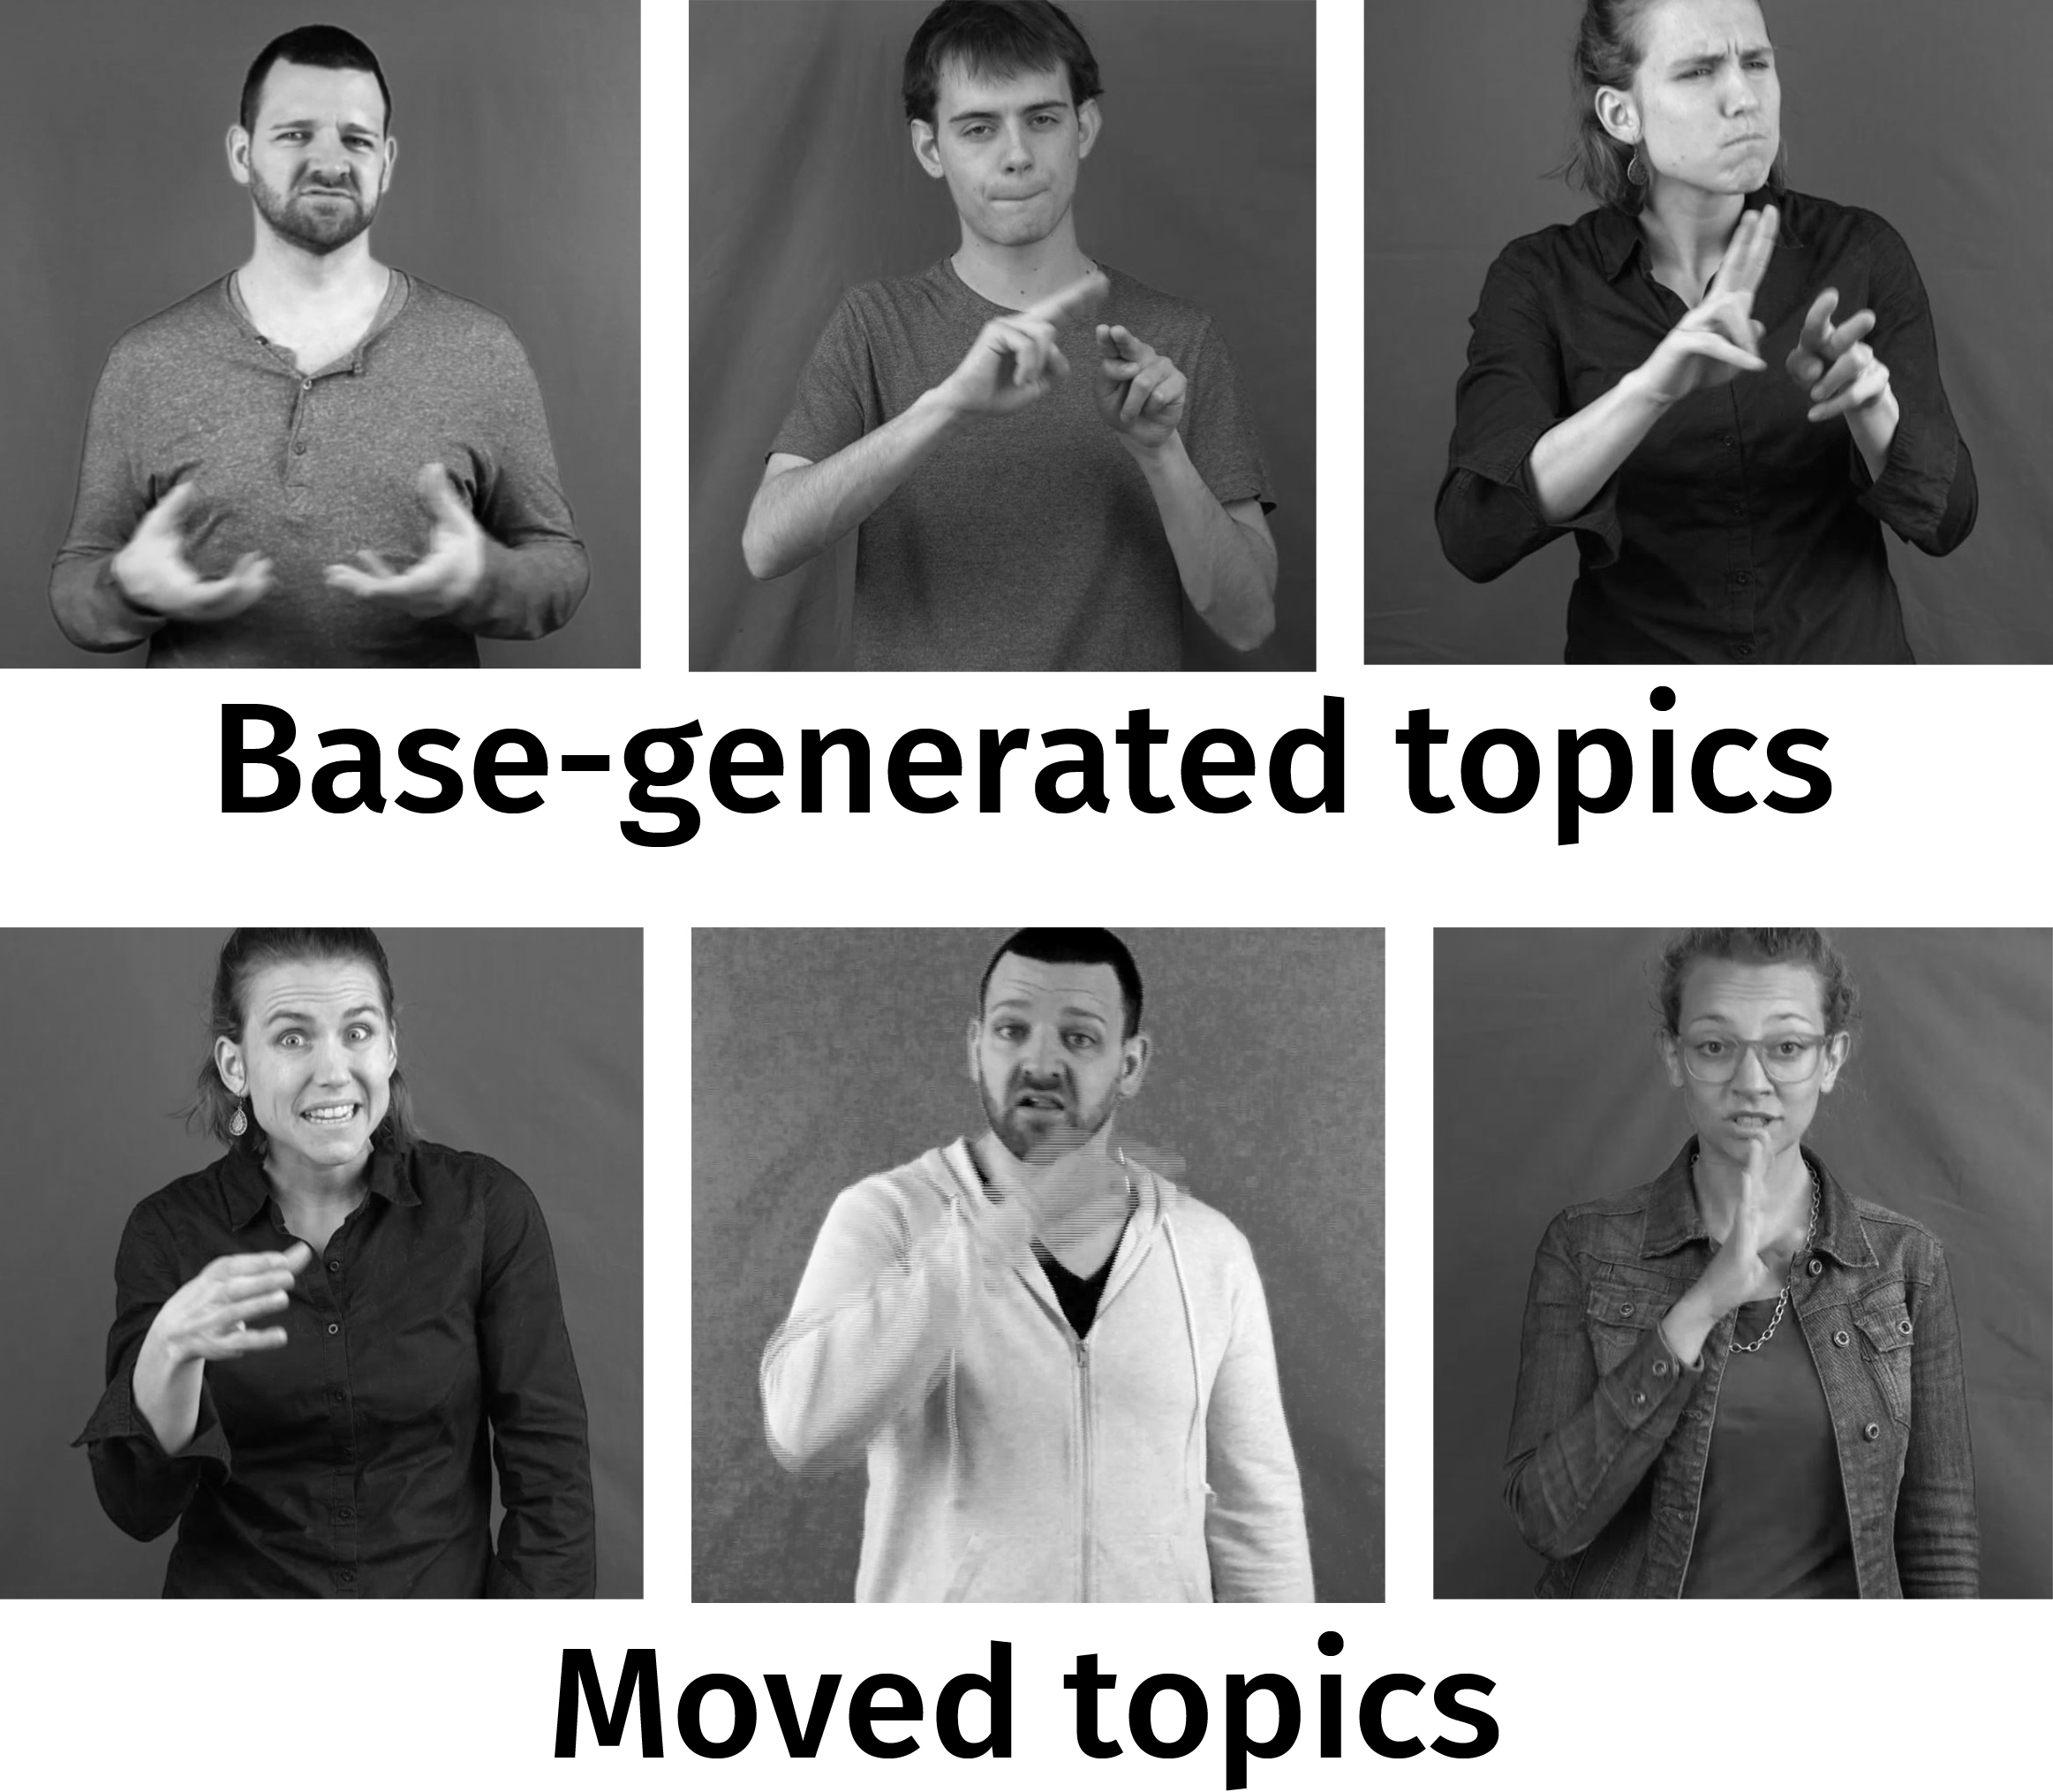
\includegraphics[width=0.9\textwidth]{topicsdgs2sw.jpg}
	\caption{The non-manual markings used for base-generated (top row) and moved topics (bottom row).}
	\label{topicsindgspicture}
\end{figure}

Topics in DGS, just like in other sign languages (see \citealt{aarons1994aspects} for \is{American Sign Language}American Sign Language or \citealt{pfau2008topics} for Sign Language of the Netherlands), can be stacked. It is unclear yet how many topics can be stacked, but due to processing limitations it seems unlikely that there would be more than two or three topics in a sentence. What is clear, however, is that a base-generated topic can be combined with another base-generated topic, as shown in (\ref{topicsindgszwozwoa}).

\begin{exe}
\ex \slg[base-top]{vegetables,} \slg[base-top]{china,} \slg{index\textsubscript{3a} person+++ broccoli eat}
%\ex {\hspace{27pt}{\small base-top}} {\hspace{-1pt}{\small base-top}} {}   \\
%{$\overline{\textrm{\textsc{vegetables}}}$,\textcolor{white}{l}} {$\overline{\textrm{\textsc{china}}}$,}  {\textsc{index}\textsubscript{3a} \textsc{person+++ broccoli eat}}     
\glt `As for vegetables, as for China, people eat broccoli there.' \label{topicsindgszwozwoa} 
\end{exe}

\noindent The example shows that the locative expression \textsc{china} receives the same non-manual marking as the base-generated topic \textsc{vegetables}. This is because \textsc{china} is not an argument of the verb. %Locatives, however, do not need this non-manual marking in any case as I will illustrate in the next subsection. 

This kind of base-generated topic stacking is, however, only possible for constituents that are not arguments of the verb. This means that an argument of the verb cannot receive the `base-top' marking, as shown in (\ref{topicsindgszwozwoamorestackinga}). 

\begin{exe} 
\ex *\slg[base-top]{vegetables,} \slg[base-top]{pepper\textsubscript{\textup{i}},}\textsubscript{\textup{i}} \slg{paul}\textit{t}\textsubscript{i} \slg{like}
%\ex {\hspace{32pt}base-top} {\hspace{6pt}base-top} {}   \\
%{*$\overline{\textrm{\textsc{vegetables,}}}$} {$\overline{\textrm{\textsc{pepper}\textsubscript{i},}}$}  {\textsc{paul} \textit{t}\textsubscript{i} \textsc{like}} 
\glt \textcolor{white}{*}`As for vegetables, as for pepper, Paul likes it.' \label{topicsindgszwozwoamorestackinga}
\end{exe}

\newpage 
\noindent When combining base-generated and moved topics, only one possibility is found. Base-generated topics have to precede moved topics and not the other way around. This is shown by the minimal pair in (\ref{nochanderemoeglichkeiten}).

\begin{exe} 
\ex\label{nochanderemoeglichkeiten}\begin{xlist}
\ex \textcolor{white}{*}\slg[base-top]{vegetables,} \slg[moved-top]{pepper\textsubscript{\textup{i}},} \slg{paul} \textit{t}\textsubscript{i} \slg{like}
%
%\ex {\hspace{32pt}base-top} {\hspace{-1pt}moved-top} {}   \\
%{\textcolor{white}{*}$\overline{\textrm{\textsc{vegetables,}}}$} {\textcolor{white}{l}$\overline{\textrm{\textsc{pepper}\textsubscript{i},}}$}  {\textsc{paul} \textit{t}\textsubscript{i} \textsc{like}} 
\glt \textcolor{white}{*}`As for vegetables, as for pepper, Paul likes it.' \label{nochanderemoeglichkeitena}

\ex *\slg[moved-top]{pepper\textsubscript{\textup{i}},} \slg[base-top]{vegetables,} \slg{paul} \textit{t}\textsubscript{i} \slg{like}
%
%\ex {\hspace{-1pt}moved-top} {\hspace{28pt}base-top}  {}   \\
%{*$\overline{\textrm{\textsc{pepper}\textsubscript{i},}}$} {$\overline{\textrm{\textsc{vegetables,}}}$} {\textsc{paul} \textit{t}\textsubscript{i} \textsc{like}} 
\glt \textcolor{white}{*}`As for pepper, as for vegetables, Paul likes it.' \label{nochanderemoeglichkeitenb}

\end{xlist}
\end{exe}

\noindent The examples in (\ref{nochanderemoeglichkeiten}) are interesting as they show that the base-generated topic seems to be in a structurally higher position than the moved topic. The examples also show that, in line with what was described earlier, base-generated/non-integrated topics are typically used as frame-setting topics (e.g., \textsc{vegetables} in (\ref{nochanderemoeglichkeitena})) and moved/integrated topics (e.g., \textsc{pepper} in \ref{nochanderemoeglichkeitena}) as aboutness topics. Additionally, the observations are in line with the idea that base-generated frame setters are structurally higher than moved aboutness topics. 


%\clearpage

\begin{digression}{Topicalization in event conditionals}{}
\noindent It has been noted in the literature than many languages, including English, do not allow topicalization in adverbial clauses. A prime example are event conditionals, cf. (\ref{eventconditionalhaegemann}) from \citet[332]{haegeman2003conditional}.

\begin{exe}
\ex *If these final exams you don't pass you won't get a degree. \label{eventconditionalhaegemann}
\end{exe}

\noindent That topicalization is not possible in event conditionals is usually explained by assuming that they exhibit a deficient left periphery (\citealt{haegeman2003conditional, haegeman2004topicalization}; but see \citealt{haegeman2013syntax} for an alternative account). However, in some languages, topicalization of this sort is possible. This is, for example, the case with Bavarian Extraction shown in (\ref{bavarianextraction}).

\begin{exe}
\ex Bavarian \citep[232]{grewendorf2015bavarian} \\ \gll {[\textit{De}} {\textit{Mass}]\textsubscript{i}} {\textit{wenn}} {\textit{i}} {t\textsubscript{i}} {\textit{no}} {\textit{drink},} {\textit{bin}} {\textit{i}} {\textit{bsuffa}.}   \\
{this} {liter} {if} {I} {} {still} {drink} {am} {I} {drunk} \\
\trans `If I drink this Mass, I will be drunk.'   \label{bavarianextraction}
\end{exe}

\noindent A similar observation can be made with regard to DGS (for similar observations regarding Sign Language of the Netherlands,\is{Sign Language of the Netherlands} see \citealt{pfau2008topics}). The example in (\ref{bavarianextractiondgsa}) shows a regular DGS event conditional. The example in (\ref{bavarianextractiondgsb}) illustrates that topicalization is, similar to Bavarian, possible. Note that the manual conditional marker \textsc{if} is optional in DGS. 

\begin{exe}
\ex\begin{xlist}  \label{bavarianextractiondgs}
\ex \slg[conditional]{(if) index_2 exam \slg[\textup{hs}]{pass}} \slg[hs]{can-neg} \slg{apprenticeship}\\
`If you don't pass the exam you won't be able to do an apprenticeship.' \label{bavarianextractiondgsa}
\ex \slg[move-top]{exam_{\textup{i}}} \slg[conditional]{(if) index_2 \textup{t}_{\textup{i}} \slg[\textup{hs}]{pass}} \slg[hs]{can-neg} \slg{apprenticeship}\\
`If you don't pass the exam you won't be able to do an apprenticeship.' \label{bavarianextractiondgsb}
\end{xlist}
\end{exe}

\noindent Is is interesting to note, however, that the left periphery of event conditionals in DGS still is truncated. This can be seen by the fact that \textit{wh}-movement is blocked in conditionals in DGS and \textit{wh}-phrases need to stay \textit{in-situ}.




%\begin{exe}
%\ex 
%\glll   {${\hspace{77}\underline{\textrm{\quad hn}}}$} \\
%{\hspace{77pt}cond}  {\hspace{10}hs} \\
%{$\overline{\textrm{\textsc{index}\textsubscript{2} \textsc{exam pass}}}$} {$\overline{\textrm{\textsc{can}}}$}  { \textsc{apprenticeship}}\\
%\glt \textcolor{white}{\%}`If you don't pass the exam you won't be able to do an apprenticeship.' \label{ex:topicconditionaldgsa}
%\end{exe}
%

\end{digression}

\is{topic|)}

\largerpage
\section{Foci}\label{generalfocussection}
\is{focus|(}
\subsection{General overview}
\label{finersplitsfocus}
\is{focus|(}
The notion of topic has to be strictly kept apart from the notion of focus, as focus, in contrast to (non-contrastive) topics, can affect truth conditions. This can be shown, for example, with focus particles like English \textit{only}. In a sentence with the focus particle \textit{only}, as in (\ref{focustrughcond}), one constituent needs to be associated with focus. In English, this is done by pitch accent, usually highlighted using small caps. Depending on which constituent is focused, the sentence is assigned different truth-conditions as can be seen from the paraphrases. %Small caps indicate pitch accent.   %While the choice of the topic does not affect truth conditions, the choice of the focus can. 



\begin{exe}
\ex\label{focustrughcond}
\begin{xlist} 
\ex John only saw $[$\textsubscript{Focus} the \textsc{play}$]$ yesterday. \\
`There is nothing apart from the play that Paul saw yesterday.'\label{ex:focustrughconda}
\ex John only saw the play $[$\textsubscript{Focus} \textsc{yes}terday$]$. \\
`There is no other day apart from yesterday on which Paul saw the play.'\label{ex:focustrughcondb}
\end{xlist}
\end{exe}

\noindent The minimal pair in (\ref{focustrughcond}) illustrates that the choice of which constituent is focused can lead to truth value changes. In this case, this is because what is focused is interpreted as relevant while other possible alternatives are excluded: ``Focus indicates the presence of alternatives that are relevant for the interpretation of linguistic expressions'' \citep[18]{krifka2007basic}. This means that the example in (\ref{ex:focustrughconda}) will get the interpretation that John saw nothing else than the play yesterday and no other alternatives (as, for example, some specific movie that was mentioned in the context). Similarly, (\ref{ex:focustrughcondb}) will get the interpretation that John saw the play on no other day than yesterday and not on any alternative day. 

While the term `topic', loosely, refers to what a sentence is about, the term `focus' refers, loosely, to new information in a sentence. In example (\ref{focustrughcond}) above, the speaker assumed that the hearer had the wrong alternatives in mind and added the correct alternative (while excluding the wrong alternatives at the same time) as new information. 

\subsubsection{Broadening the picture: two definitions of focus}
Of course, focus is not restricted to \textit{only} foci and a broader picture is needed. Focus is, for example, also used in answers to questions, as the answer to a question has to be, by definition, new to the hearer. Following \citet{rooth1996focus}, we can say that the focus in an answer to an alternative question correlates to the position of the disjoint alternatives. For \textit{wh}-questions, focus correlates with the position of the \textit{wh}-element. This is shown in (\ref{rooth1996}), from \citet{rooth1996focus}. There are two questions in the illustration, an alternative question (on the left) and a \textit{wh}-question (on the right). Although both answers at the bottom of the illustration are made up of the same lexical material they cannot be used interchangeably. The answers corresponding to the questions of which they would be considered appropriate are linked by solid lines, the dashed lines show inappropriate question-answer pairs. 

\begin{exe}
\ex\label{rooth1996} 
%\begin{figure}
%\centering
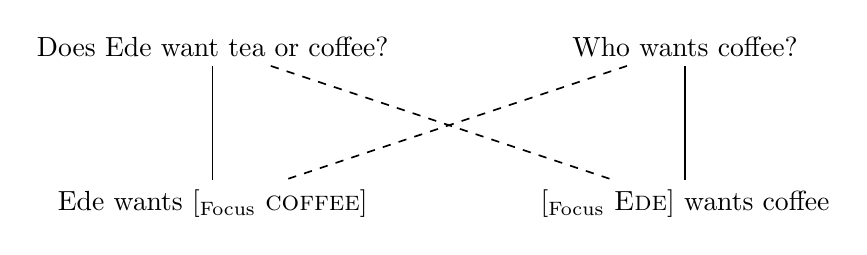
\begin{tikzpicture}[baseline={([yshift={-2.3ex}]current bounding box.north)}, scale=1.00]
\tikzset{level 1+/.style={sibling distance=2\baselineskip}}
%\Tree [.DP [.D the ] [.NP man ]]
\node (a) at (0,0) {Does Ede want tea or coffee?} ;
\node (b) at (6,0) {Who wants coffee?} ;

\node (c) at (0,-2) {Ede wants $[$\textsubscript{Focus} \textsc{coffee}$]$} ;
\node (d) at (6,-2) {$[$\textsubscript{Focus} \textsc{Ede}$]$ wants coffee} ;

\draw[semithick, -] (b) to (d);
\draw[semithick, -] (a) to (c);
\draw[semithick, -,dashed] (b) to (c);
\draw[semithick, -,dashed] (a) to (d);
%\draw[help lines] (-4,-4) grid (4,4)
\end{tikzpicture}
%\caption{Question-answer congruence for focus (after Rooth 1996).}
%\end{figure}
\end{exe}

\noindent What (\ref{rooth1996}) shows is that when a speaker asks if Ede wants coffee or tea, the fact that Ede wants something is already established. What the speaker consequently assumes is that what Ede wants to drink will be new to the asker and is thus in focus. It would not be felicitous to focus \textit{Ede}, since the fact that he wants something is already known. Similarly, when it is asked who it is that wants coffee, the newsworthy information is the name of the referent that wants to drink something. 

Note that we have two definitions of focus now: One that is about alternatives and one that is about new information. So while, for example, \citet[18]{krifka2007basic} states that focus is the indication of alternatives relevant to the interpretation, \citet[1876]{hinterwimmer2011formation} defines focus as that ``part of the sentence that conveys the information the speaker wishes to represent most prominently and onto which s/he wants to draw the hearer's attention.'' Both definitions do not contradict each other. Focus does evoke alternatives that are viewed as relevant to the speaker, the alternative that is highlighted is highlighted because the speaker assumes that this alternative is new to the hearer: to highlight something always means to highlight something with respect to something else (and these are the alternatives).\footnote{To be more precise, it is not the alternative itself that needs to be new to the hearer but the relation of the alternative to the rest of the proposition. Consider the example in (\ref{kissmotherrelation}), from \citet[55]{rochemont2016givenness}. From the example it becomes clear that \textit{John} can be focused, although it is already given in the context.

\ea A: Who did John's mother kiss? \\
B: She kissed \textsc{John}. \label{kissmotherrelation}
\z

\noindent This is possible as the new information is the relation John has with the kissing event.

}


\subsubsection{Focus and presupposition versus topic and comment}
Everything that is not focused in a sentence is called the `presupposition' or the `background'. The proposal to divide focus and background goes back to \citet{jackendoff1972semantic} who defines the focus of a sentence as ``the information in the sentence that is assumed by the speaker not to be shared by him and the hearer'' and presupposition respectively as ``the information in the sentence that is assumed by the speaker to be shared by him and the hearer'' \citep[230]{jackendoff1972semantic}.\footnote{The knowledge that is shared by the interlocutors is usually called the `common ground' \citep{stalnaker1978assertion}.}

Although a sentence can be split up into a topic and a comment part, with the topic referring to old information and although the focus refers to new information, focus and comment are not the same. This is because the terms refer to different levels of information structure. This can be explained best by means of an example. In many cases, the topic of a sentence and its presupposition on the one hand, and the focus and the comment on the other hand, coincide. This is illustrated in the example dialogue in (\ref{topicfocusdistincitona}), taken from \citet[467]{vallduvi1996linguistic}.

\begin{exe}
\ex\label{topicfocusdistincitona}
A: What about John? What does he do? \\
B: John drinks \textsc{beer}.
\end{exe}

\noindent The information structure of Bob's answer to Alice's question can be represented in terms of topic and comment (\ref{ex:topicfocusdistincitonba}) and in terms of focus and presupposition (\ref{ex:topicfocusdistincitonbb}). From the two representations it looks as if we could conflate the four notions and equate topic with presupposition and focus with comment.

\begin{exe}
\ex\label{topicfocusdistincitonb}\begin{xlist} 
\ex $[$\textsubscript{Topic} John$]$ $[$\textsubscript{Comment} drinks \textsc{beer}$]$ \label{ex:topicfocusdistincitonba}
\ex $[$\textsubscript{Presupposition} John$]$ $[$\textsubscript{Focus} drinks \textsc{beer}$]$ \label{ex:topicfocusdistincitonbb}
\end{xlist}
\end{exe}

\noindent There are, however, examples that show that this is not always the case. The information structure of Bob's answer in (\ref{topicfocusdistincitona}) is mainly determined by Alice's question. As her first question is about John, John has to be given. Her second question is about the action John performs. What exactly this action is, is left open. If we change Alice's question and make it more specific, the difference between topic and presupposition as well as the difference between focus and comment is more obvious, as shown in the example dialogue in (\ref{topicfocusdistincitonc}), again taken from \citet[468]{vallduvi1996linguistic}.

\begin{exe}
\ex\label{topicfocusdistincitonc}
A: What about John? What does he drink? \\
B: John drinks \textsc{beer}.
\end{exe}

\noindent Note that what changed in the dialogue in (\ref{topicfocusdistincitonc}) is not Bob's answer, but only Alice's question. She is now asking something more specific, namely, what John is drinking. Therefore, the drinking is already given and therefore cannot be in the focus of Bob's answer, but it is part of the presupposition. Additionally, John is also in the presupposition, since Alice also asked about John. Nevertheless, John is also what Bob's sentence is about, hence John is also the topic of the sentence. The only thing left now is the beer. The beer is the only new information that is provided by Bob, so it is the focus. We arrive at the following structure:

\begin{exe}
\ex\label{topicfocusdistincitond}\begin{xlist} 
\ex $[$\textsubscript{Topic} John$]$ $[$\textsubscript{Comment} drinks \textsc{beer}$]$ \label{ex:topicfocusdistincitonbaa}
\ex $[$\textsubscript{Presupposition} John drinks$]$ $[$\textsubscript{Focus} \textsc{beer}$]$ \label{ex:topicfocusdistincitonbbb}
\end{xlist}
\end{exe}

\noindent The representation given in (\ref{ex:topicfocusdistincitonbaa}) shows that the topic-comment structure has not changed. Bob's answer is still a sentence about John, about whom it is commented that he drinks beer. What has changed, however, is the focus-pre\-sup\-posi\-tion structure. That John drinks something is presupposed by Alice's question. What is new, i.e., what is the focus of the sentence, is that it is beer that he drinks. 

\subsubsection{The syntax of focus: two structural positions}
While there are (at least) two topic positions in the CP area, as discussed in the previous section, there is only one focus position. Nevertheless, two types of focus with two different structural positions can be differentiated. These two types are called contrastive (or: identificational) and information focus (see \citealt{kiss1981structural}). Contrastive focus is exhaustive, i.e., it selects an item from a larger set of items and is used for contrasts and corrections. Information focus needs not be exhaustive. It is used as an answer to a \textit{wh}-question as was already introduced on page \pageref{rooth1996} (see the example in (\ref{rooth1996})). 

Languages use different strategies to mark constrastive focus. Some languages, for example, English, use cleft structures and intonational means to mark contrastive focus, as shown in (\ref{constrativefocusexample}). Other languages, for example Bulgarian, do not only prepose topics, but also foci -- without using a cleft strategy. In cases in which a topicalized and a focalized element occur in one clause, we find the topic preceding the focus, as shown in the Bulgarian example from \citet[72]{van1995focus} in (\ref{constrativefocusexamplebulgarian}).\footnote{An interesting feature in Bulgarian is that the focus head is realized overtly with the focus marker \textit{li}. }

\begin{exe}
\ex A: Why did Sarah buy so much beer?\\
B: It was \textsc{Lorenz} who bought the beer. \label{constrativefocusexample}
\end{exe}

\begin{exe}
\ex Bulgarian \citep[72]{van1995focus} \\ \gll {\textit{Filma}} {\textit{Marija}} {\textit{li}} {\textit{gleda?}}  \\
{film} {Marija} {\textsc{foc}} {watch} \\
\trans `As for the film, it is Marija who is watching it?'   \label{constrativefocusexamplebulgarian}
\end{exe}

\noindent From data like the Bulgarian one, it was argued that these two types of focus are located in two different structural positions: a high, CP-internal position for contrastive focus and a low, IP-internal position for (new) information focus (see, for example, \citealt{beninca2001position}; \citealt{benincapol2004topic}; \citealt{belletti2004aspects}; \citealt{belletti2003i}). This is summarized in Table \ref{ldhtdiff}.

\begin{table}
\fittable{
\begin{tabular}{lll}
\lsptoprule
 & Contrastive focus & Information focus \\\midrule
Usage & Exhaustive identification & Marking information as being non-presupposed \\
Behavior & Optional & Present in every utterance \\
Movement & Yes & No \\
%\rowcolor[gray]{.9}
%Binding effects & Yes & No \\
%Island sensitive & Yes & No \\
%\rowcolor[gray]{.9}
%Intonational break & No & Yes \\
\lspbottomrule
\end{tabular}
}
\caption{Some differences between contrastive and information focus (based on \citealt{kiss1998identificational})\label{ldhtdiff}}
\end{table}
\is{focus|)}


\subsection{Foci in sign languages}
While research on sign languages has shown, mainly for \is{American Sign Language}American Sign Language, that topics appear in a clause-initial position, the position for foci seems to be a different one. The position for focused elements (or more general: new information) in American Sign Language is clause-final rather than clause-initial \citep{wilbur1991intonation, wilbur1994foregrounding, wilbur1996evidence, wilbur1997prosodic}. Similar observations have been made for other sign languages, including, for example, \is{Brazilian Sign Language}Brazilian Sign Language \citep{de1999phrase} and Sign Language of the Netherlands\is{Sign Language of the Netherlands} \citep{crasbornkoijiros2012}. 

\citet[92]{wilbur1997prosodic} illustrates clause-final focus in American Sign Language with modals which occur preverbally in the language when unfocused. When focused, however, they appear in a clause-final position, as shown in (\ref{focusedmodalronnie}).

\begin{exe}
\ex American Sign Language \citep[92]{wilbur1997prosodic} \\ % {\hspace{105pt}br}   \\
{\textsc{\dots\ but stay home all-day everyday can't}}
\glt `\dots\ but I \textsc{can't} stay home all day everyday.' \label{focusedmodalronnie}
\end{exe}

\noindent Three analyses were offered for this clause-final focus position: leftward movement, rightward movement, and \is{focus doubling} doubling with deletion: \citet{wilbur1997prosodic}, for example, suggests that non-focus material is preposed, i.e., moved to the left. Others, e.g., \citet{petronio1993clause}, have suggested the focused elements are moved to the right, maybe involving an additional step of doubling the focused element with subsequent deletion of the clause-internal copy. It is not clear yet which of these analyses should be preferred.  

Another\is{focus doubling} example illustrating that focused elements appear in a clause-final position in American Sign Language are doubling constructions. In American Sign Language, as in many other sign languages, several elements that originally appear in a clause-internal position can be doubled in a clause-final position. This is, for example, possible with modals as shown in (\ref{doublingaslmodals}) from \citet[135]{petronio1993clause}.\footnote{Other elements that can be doubled in American Sign Language include quantifiers, negatives, and \textit{wh}-signs \citep{petronio1993clause}.}

\begin{exe}
\ex \slg[pol]{ann will leave will}
%\ex {\hspace{105pt}pol}   \\
%{$\overline{\textrm{\textsc{ann will leave will}}}$} 
\glt `Will Ann leave?' \label{doublingaslmodals}
\end{exe}

\noindent The second, `doubled' modal in examples like the one in (\ref{doublingaslmodals}) usually receives focus given that it is prosodically prominent. In some sign languages, for example in \is{Brazilian Sign Language}Brazilian Sign Language, the doubles receive head nods \citep{de1999phrase}. The claim that doubling is related to focus is supported by the fact that there can only be one double per clause. Additionally, an element, such as a modal, cannot be doubled in a \textit{wh}-question. As \textit{wh}-phrases are thought to be located in FocP (or at least to move through FocP), it is reasonable to assume that the clause-final double is located in FocP. 

It is usually argued that the double is located in the head of the focus phrase as only single signs, i.e., heads, can be doubled. We could thus assume either a right-headed FocP or a left-headed and left-branching FocP with an additional remnant movement step that moves the clause to the left of the Foc\textdegree\ (in the specifier of the FocP).  

While doubling only involves heads, there are other constructions in which phrases occur in a clause-final position. \label{pseudocleeeeefts}A common strategy of overt syntactic focusing in \is{American Sign Language}American Sign Language are pseudo-clefts. This construction, traditionally called `rhetorical question structure', is illustrated in (\ref{wilburrqanp}).

\begin{exe}
\ex American Sign Language \citep[92]{wilbur1997prosodic} \\ \slg[br]{find\#out what,} \slg{stay home can't}
%\ex {\hspace{82pt}br} {}   \\
%{$\overline{\textrm{\textsc{find\#out what}}}$,} {\textsc{stay home can't}}
\glt `What I discovered is that \textit{I can't stay home}.' \label{wilburrqanp}
\end{exe}

\noindent \citet{wilbur1997prosodic} argues that in these constructions, the first part of pseudo-cleft structures, as in (\ref{wilburrqanp}), which are accompanied by a brow raise, is the non-focused part consisting of an open proposition and the second part of the structure represents the focused material (see also \citealt{wilbur1994foregrounding, wilbur1996evidence}). An alternative account on this construction is presented by \citet{caponigro2011ask} who, similar to \citet{wilbur1996evidence}, assume that the structure forms a syntactic and semantic unit. Their account, however, is different from \citeauthor{wilbur1996evidence}'s as they argue that the question constituent receiving the brow raise is an embedded interrogative clause and the answer constituent is an embedded declarative clause with the whole structure being a declarative clause. 

Concerning the non-manual markers used for focus marking, the literature mainly reports head nods and raised eyebrows  as well as shoulder movements. The shoulders were found to play a role, for example, in contrastive focus in \is{American Sign Language}American Sign Language \citep{wilbur1999syntactic} as well as in \is{Sign Language of the Netherlands}Sign Language of the Netherlands \citep{crasborn2013phonology}.

\subsection{Foci in DGS}
In this section, I will give a brief overview of the focusing strategies used in DGS. In line with the literature, I will show that information focus mainly stays unmarked. As in other sign languages, DGS exhibits focus doubling and pseudo-clefts which are marked in a similar manner as in American Sign Language. Concerning contrastive focus I will show that the non-manual marking which is used is subject to dialectal variation as signers from Baden-Württemberg and signers from Bavaria use different strategies. Finally, I will briefly discuss the role of signing space and shoulder positions in contrastive focus. For the use of focus particles in DGS, which will not be discussed here, I refer the reader to \citet{herrmann2013modal}.

\subsubsection{Information focus}
With information focus\is{information focus} we do not find any reordering (i.e., movement) of manual constituents. On the whole, it information focus is usually left unmarked (see also \citealt{waleschkowski2009}). When it is marked, wide-open eyes, a short eyebrow raise, and a slight downward movement of the head or a head-nod on the focused constituent can be observed (see also \citealt[396]{happ2014vork}). This is shown in the example in (\ref{ex:informationfocusnewexample}).

\begin{exe}
\ex\label{ex:informationfocusnewexample}
A: Who did you meet yesterday?\\
\textcolor{white}{B: }\slg{yesterday} \slg[foc]{paul} \slg{meet}
%{} {\textcolor{white}{B: \textsc{yesterdayml}}foc} {}   \\
%{B: \textsc{yesterday}} {$\overline{\textrm{\textsc{paul}}}$} {\textsc{meet}}      
\glt \textcolor{white}{B: }`I met \textsc{Paul} yesterday.' 
\end{exe}

\noindent Wide information focus can also be marked by wide-open eyes and raised eyebrows spreading over the whole clause. This is illustrated in (\ref{ex:wideinformatiofocus}) -- although in most cases, wide focus stays unmarked. %However wide information focus mainly stays unmarked.

\begin{exe}
%\ex What happend?\label{ex:informationfocusdgspapaspyrou}\begin{xlist} 
\ex
A: What happened? \\
B: \slg[foc]{poss\textsubscript{1} beer fall-down}
%
%{\hspace{129pt}foc}    \\
%%{\hspace{\fill}foc} \\
%{B: $\overline{\textrm{\textsc{\textsc{poss}}\textsubscript{1} \textsc{beer fall-down}}}$}  
\glt \textcolor{white}{B: }`My beer fell down.' \label{ex:wideinformatiofocus}

\end{exe}

\noindent Taken together, if information focus is marked at all, it is marked by wide-open eyes and slightly raised eyebrows. 



\subsubsection{Focus doubling}\is{modal doubling|see{focus doubling}}\is{focus doubling}\is{doubling|see{focus doubling}}
As described for \is{American Sign Language}American Sign Language, several elements can undergo doubling in DGS, including \textit{wh}-signs (see Section \ref{whinterrogativedgs}), pronouns (see Section \ref{polarinterrogativesdgs}), and modals verbs (see Section \ref{modaldoubling}). As in other sign languages, the items undergoing doubling are heads and not full phrases (but see Section \ref{whinterrogativedgs} for evidence that this is different for \textit{wh}-doubling). In many (but not all) cases, the clause-final double receives stress, as shown in (\ref{modaldoublingdgsexample}). 

\begin{exe}
\ex \slg{paul can swim} \slg[foc]{can}
%{} {\hspace{97pt}foc}    \\
%{\textsc{paul can swim}} {$\overline{\textrm{\textsc{can}}}$}
\glt `Paul \textsc{can} swim.' \label{modaldoublingdgsexample}
\end{exe}

\noindent If we assume that the double is hosted in a head we could either assume FocP to be right-headed or that the non-doubled lexical material has moved to a left-branching specifier -- probably SpecFocP. However, another possibility is that doubling is not related to focus, at least not to contrastive focus. Instead, it seems plausible to me that it is used as an emphasis device, but I will not pursue this option any further (but see \citealt{wilbur2012informationstructure}).



\subsubsection{Pseudo-clefts}\is{pseudo-cleft}\is{wh-cleft@\textit{wh}-cleft|see{pseudo-cleft}}\is{cleft|see{pseudo-cleft}}
Similar to what was described for American Sign Language, pseudo-clefts are possible in DGS (cf. \citealt[397]{happ2014vork}). As with American Sign Language, the non-focused material can receive a brow-raise (glossed `cleft' in the example). The focused phrase in the clause-final position can receive non-manual focus marking that can be either a brow-raise or a backwards head tilt, sometimes accompanied by a nod. An example is given in (\ref{whcleft}).% which is additionally depicted in Figure \ref{pseudocleft}.

\begin{exe}
\ex \slg[cleft]{paul break what} \slg[(foc)]{vase}
%\ex {\hspace{80pt}cleft} {\hspace{14pt}foc}   \\
%{$\overline{\textrm{\textsc{paul break what}}}$,} {$\overline{\textrm{\textsc{vase}}}$}
\glt `What Paul broke was \textsc{the vase}.' \label{whcleft}
\end{exe}

\noindent According to \citet[397]{happ2014vork} the first part of cleft-structures like the one in (\ref{whcleft}) receive a topic-marking, i.e., raised eyebrows. This is in line with my own observations. Similar to the description in \citet[397]{happ2014vork}, the focus marking can be, and usually is, absent. Both possibilities are depicted in Figure \ref{pseudocleft}. In the top example the focus marking on \textsc{beer} is missing, in the bottom example, the focus marking is present (an additional brow-raise). The premise for the focus marking to be present seems to be that it marks new or unexpected information. While the top example would be felicitous at the beginning of a talk (when everyone knows that a talk about beer will follow), the second example was elicited in a context in which the signer was reporting that he will visit a talk about beer (`I'm going to a talk. The topic of the talk is beer').\footnote{This difference is also mirrored in constituent order in the examples.} Pseudo-clefts in DGS need further attention in the future. In my mind, it is not clear yet if they are really best analyzed as focus structures, but as topic-comment structures as similar constructions in the spoken language research tradition were indeed analyzed this way (e.g., \citealt{prince1978,gast2014}; see also \citealt{caponigro2011ask} for a similar point for \is{American Sign Language}American Sign Language).

\begin{figure}[bt]
\centering
	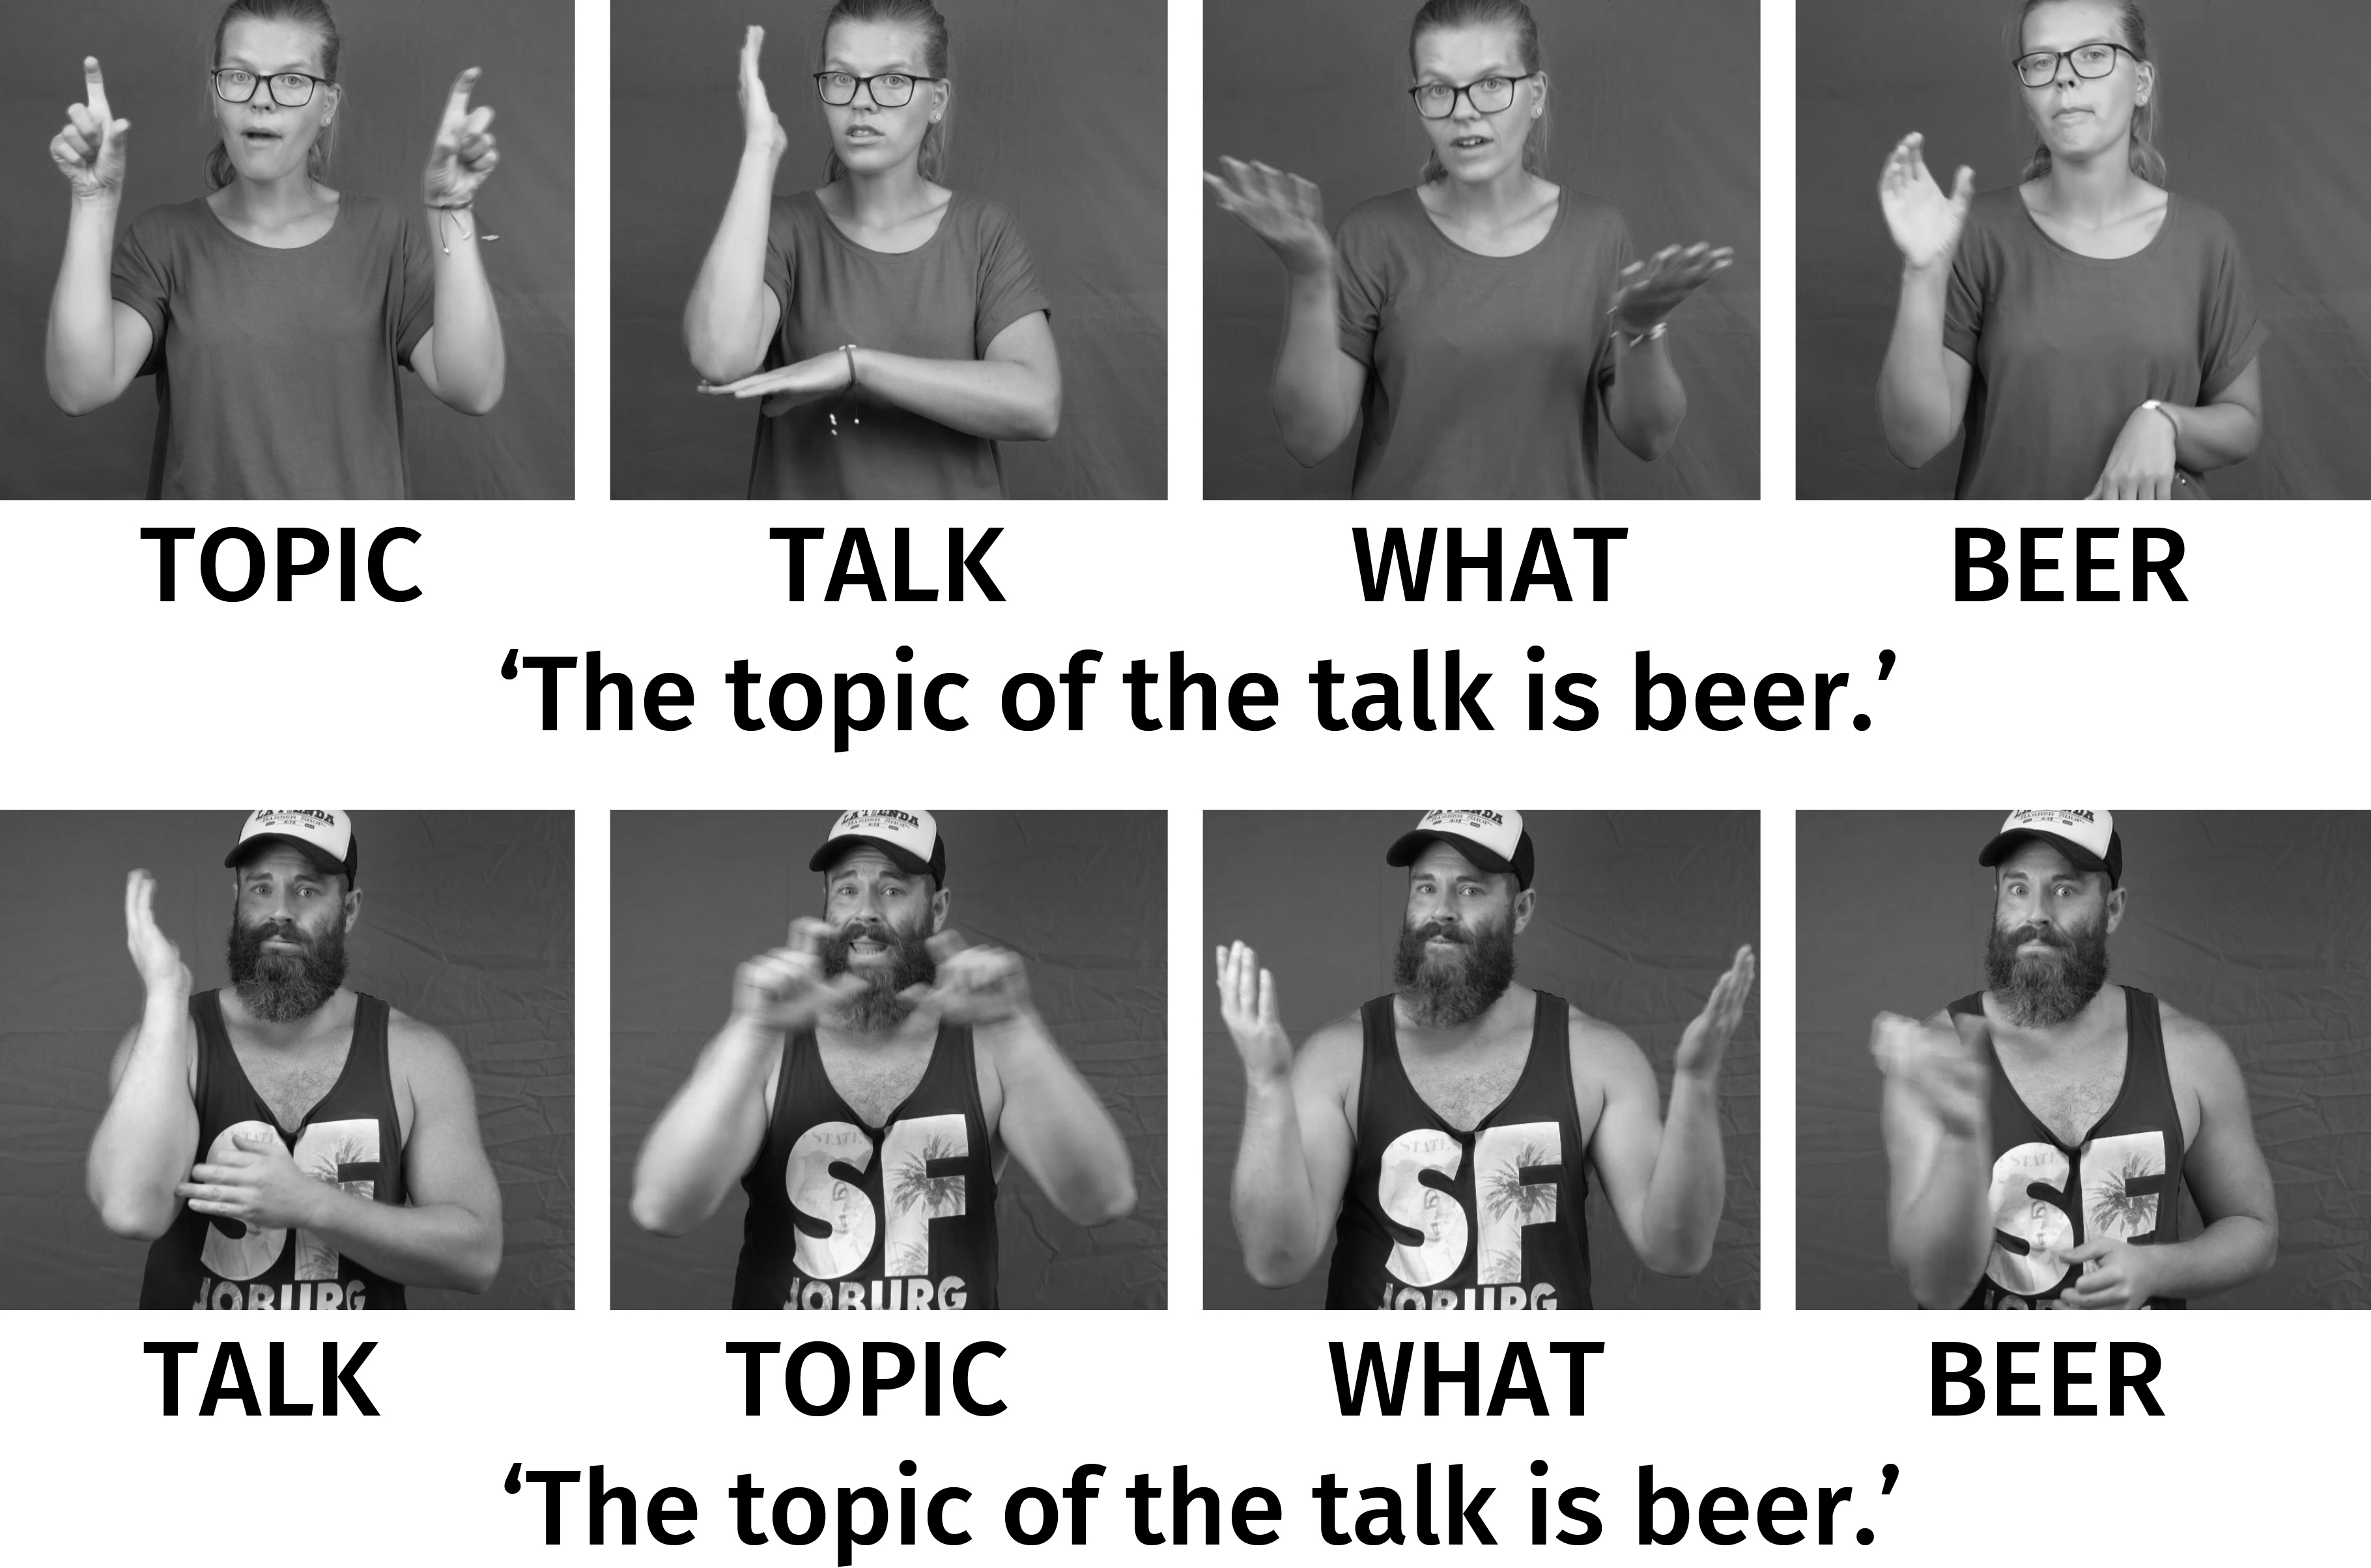
\includegraphics[width=1.0\textwidth]{pseudoclefttwosw.jpg}
	\caption{Two pseudo-clefts: one without and one with focus marking.}
	\label{pseudocleft}
\end{figure}

\largerpage
\subsubsection{Contrastive focus}\label{contrastivefocussubection}
Previous\is{contrastive focus} research on focus in German Sign Language has noted that contrastive focus is marked mainly by head nods \citep{waleschkowski2009}. \citet[402--403]{happ2014vork} also report that the non-manual marking for information and contrastive focus is the same and thus is achieved by nods (except for pseudo-clefts which are described above). This only partly matches with my own observations. 

With contrastive focus I found a unique bundle of non-manual markers that consist either of the head tilted backward and raised eyebrows or of a forward head-bow or chin-down with furrowed brows. The question of which of these non-manuals are used is subject to dialectal variation. While signers from Baden-Württemberg systematically used head-tilts and eyebrow-raises, the chin-down pattern was used by the Bavarian signers. This is shown in Figure \ref{contrastivefocus}. In both cases, the non-manuals accompany the whole constituent being contrasted.

\begin{figure}[bt]
\centering
	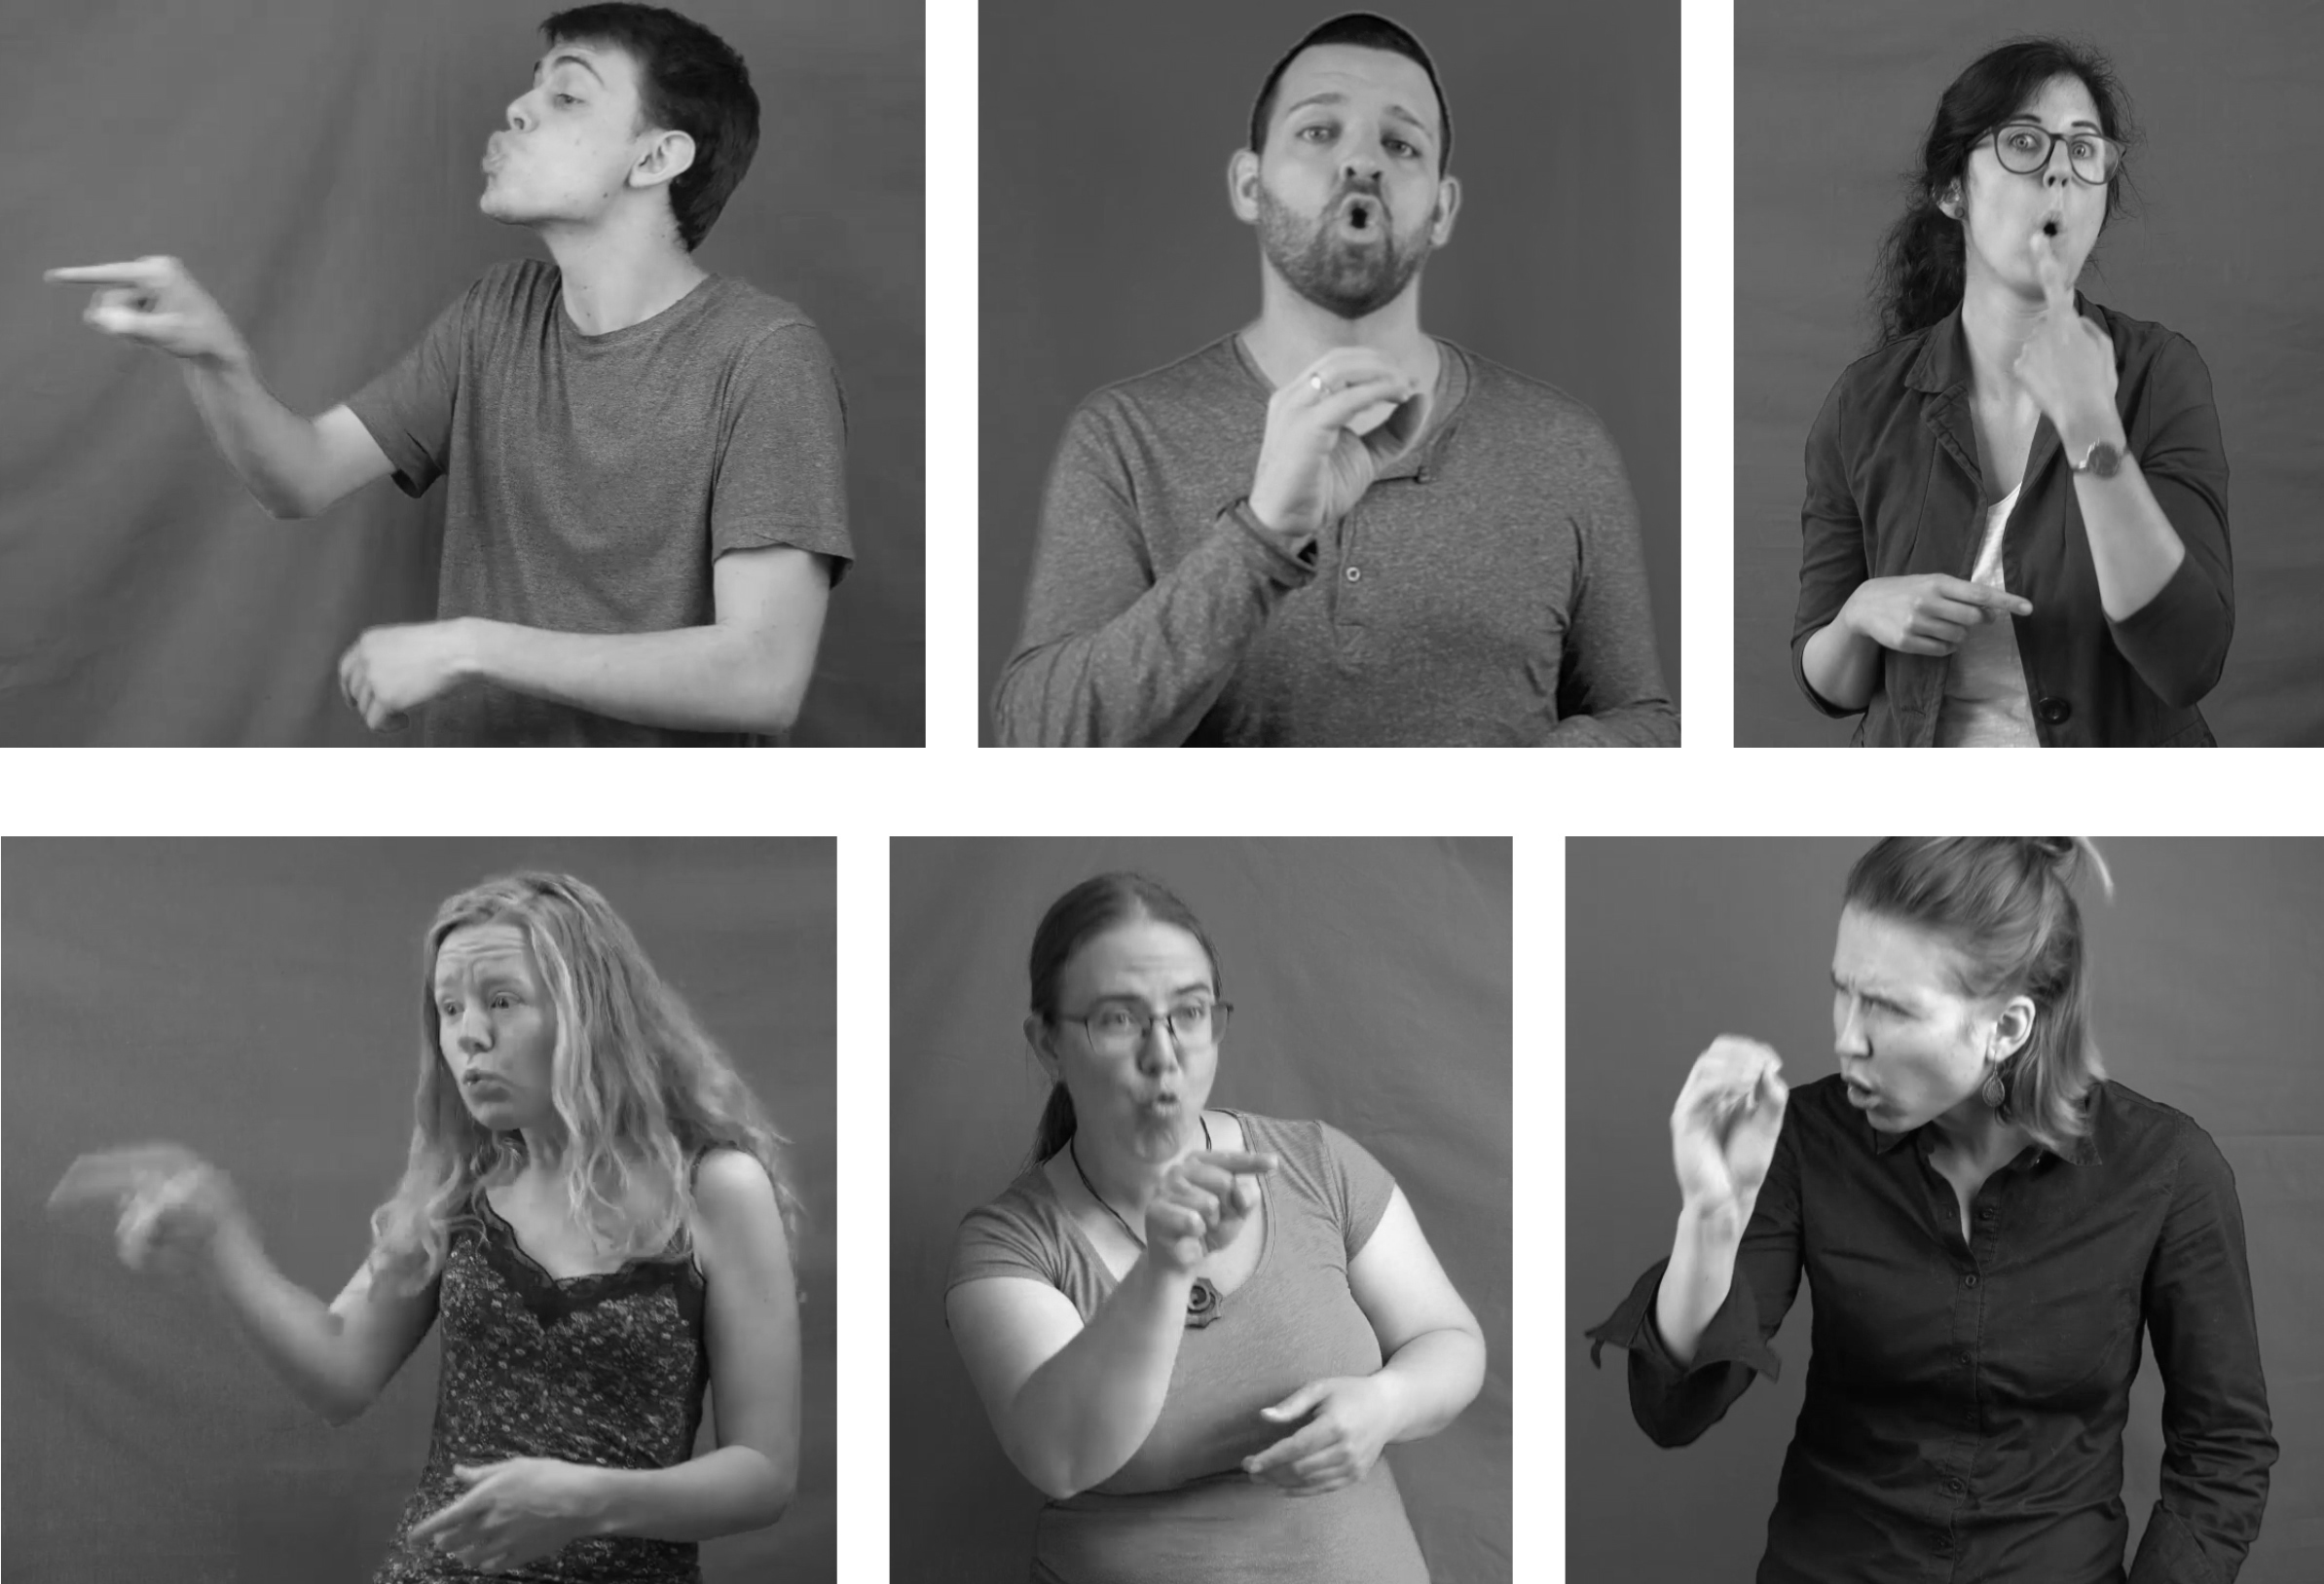
\includegraphics[width=1.0\textwidth]{contrastivefocus2sw.jpg}
	\caption{The non-manuals used with contrastive focus. Signers in the top row of the figure are from Baden-Württemberg, signers in the bottom row are from Bavaria.}
	\label{contrastivefocus}
\end{figure}

Contrastive focus can stay \textit{in-situ} in DGS, but can also be moved into a clause-initial position. Glossed examples are shown in (\ref{ex:contrastivefocusa}). The contrastive focus non-manuals are glossed `contr'.

\begin{exe}
\ex\label{ex:contrastivefocusa}\begin{xlist}
\ex
A: Paul bought beer yesterday. \\
B: \slg{yesterday} \slg[contr]{otto} \slg{beer buy}
%
%{} {\hspace{85pt}contr} {}   \\
%{B: \textsc{yesterday}} {$\overline{\textrm{\textsc{\textsc{otto}}}}$ \textsc{beer buy}}  
\glt \textcolor{white}{B: }`It was Otto who bought the beer yesterday.' \label{ex:contrastivefocusaa}
\newpage
\ex
A: Paul bought beer yesterday. \\
B: \slg[contr]{otto} \slg{yesterday beer buy}
%
%{\hspace{18pt}contr} {}   \\
%{B: $\overline{\textrm{\textsc{\textsc{otto}}}}$ {\textsc{yesterday beer buy}}}  
\glt \textcolor{white}{B: }`It was Otto who bought the beer yesterday.' \label{ex:contrastivefocusab}


\end{xlist}
\end{exe}

\noindent Future research will have to check if there is a difference -- maybe in exhaustiveness -- between moved and \textit{in-situ} contrastive focus. If this is not the case, one could assume that movement in the \textit{in-situ} cases only takes place at LF.

Taken together, contrastive focus is marked non-manually with the whole head and, in line with the bodily mapping hypothesis, with the eyebrows, although there is geographical variation with contrastive focus marking.

\subsubsection{Shoulder positions for contrasts}
As has been\is{shoulder positions} reported for other sign languages, contrastive focus is sometimes additionally marked by using the shoulders and locations in signing space. When two referents are contrasted, one is signed on one side on the body and the item to be contrasted on the other side. This is exemplarily shown in Figure (\ref{contrastiveshoulders}).


\begin{figure}[bt]
\centering
	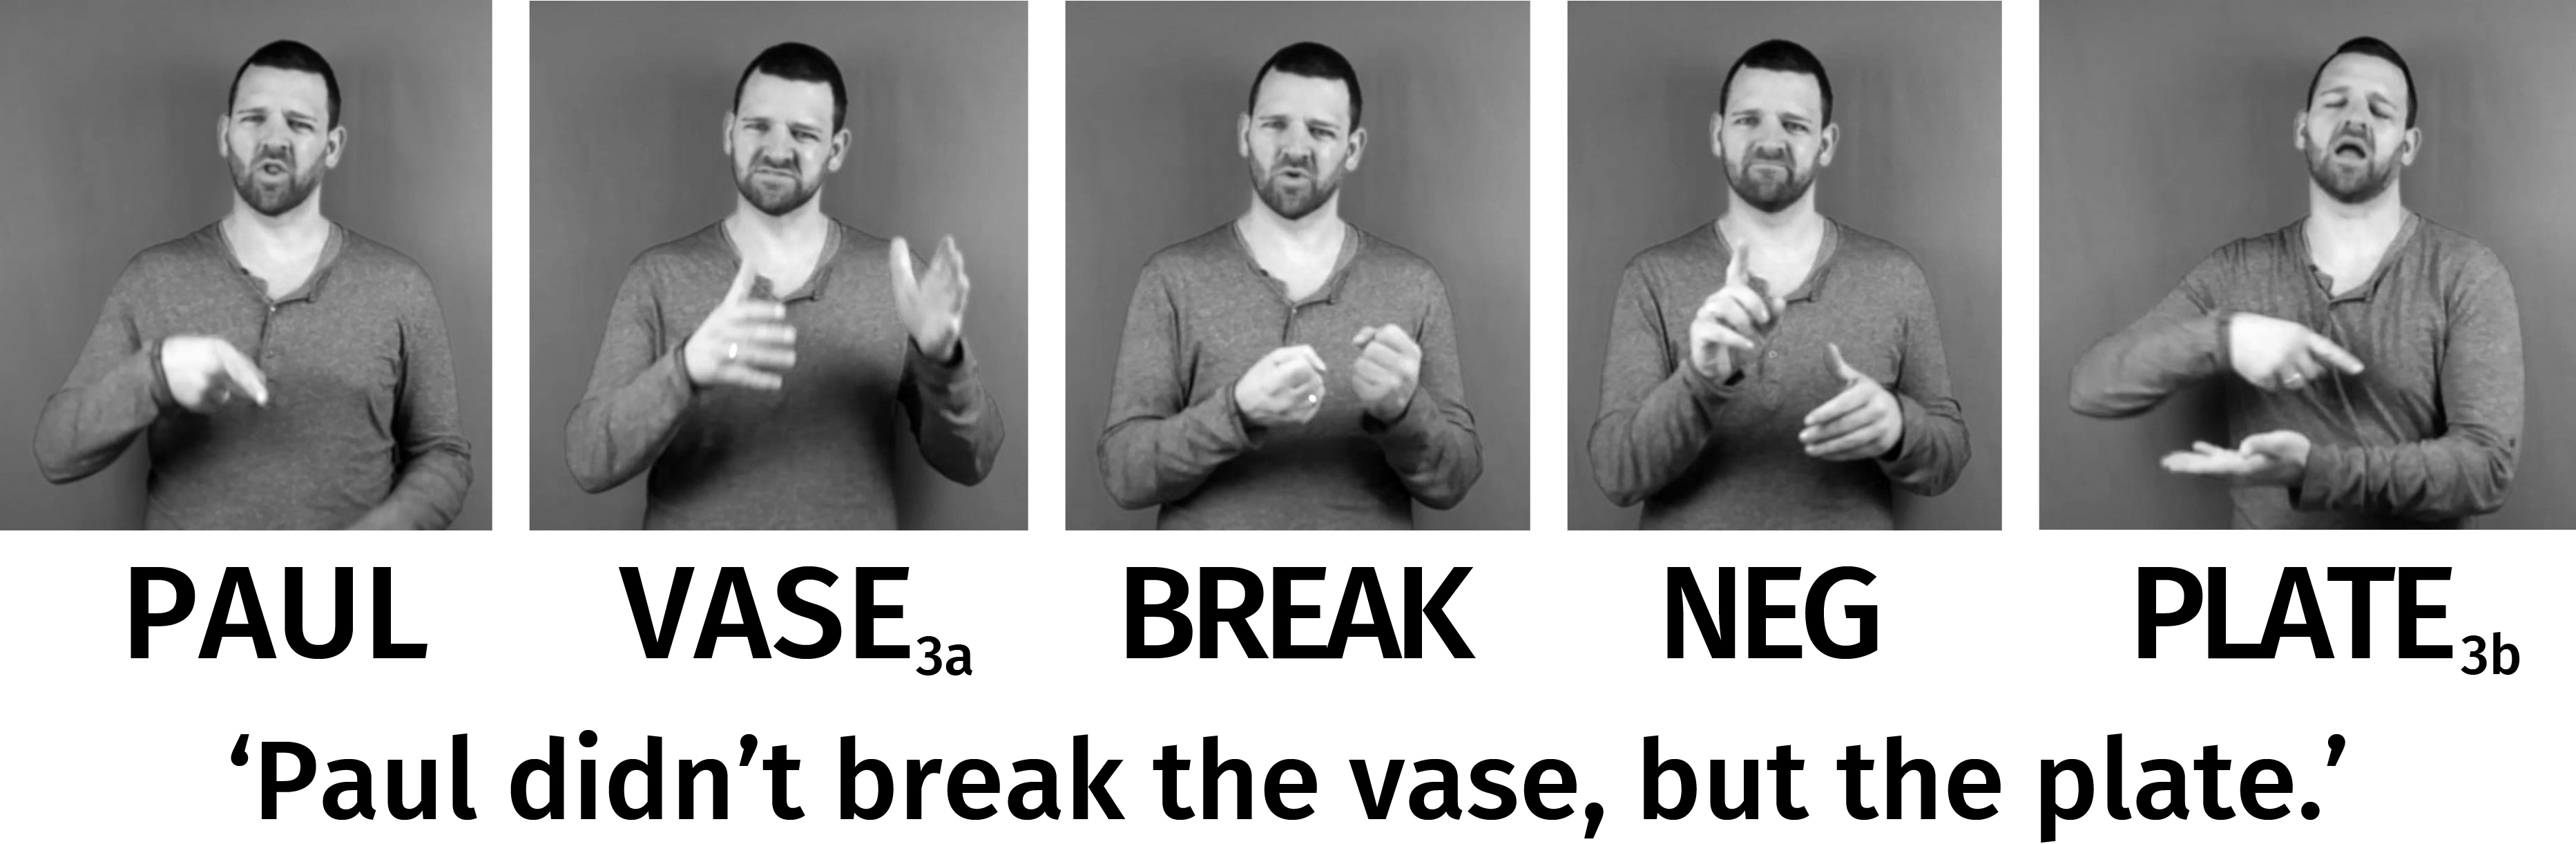
\includegraphics[width=1.0\textwidth]{contrastiveshoulderssw.jpg}
	\caption{An example of the use of signing space for contrasts.}
	\label{contrastiveshoulders}
\end{figure}

The example in the figure shows a sentence in which a vase is contrasted with a plate. While the signer locates the vase to his left in the example, the plate is located to his right. This is also mirrored by shoulder movement. This kind of opposition, however, is found in many other constructions, including plain coordination. 



Taken together, the structure of the focus phrase could be modeled in the way shown in (\ref{ex:focusphrasedgs}) if one allows heads to be right-branching. The other option would be to assume a left-headed focus phrase and additional XP movement into a higher specifier position.

%\begin{exe}
%\ex\label{ex:focusphrasedgs} 
%\begin{tikzpicture}[baseline=(current bounding box.north), scale=1.00]
%\tikzset{level distance=35pt,sibling distance=5pt,every tree node/.style={align=center,anchor=north}}
%
%\Tree [.FocP [.SpecFocP ] [.{$\overline{\textrm{Foc}}$} [.IP \edge[roof]; \node(t){\qquad \qquad}; ] [.{Foc\textdegree } ] ] ]
%\end{tikzpicture}
%\end{exe}

\begin{exe}
\ex\label{ex:focusphrasedgs} 

\begin{forest}
for tree={s sep=25mm, inner sep=0, l=12mm} %s sep = Breite; l = Höhe
[FocP [SpecFocP ] [{$\overline{\textrm{Foc}}$} [IP [{\qquad \qquad \qquad \qquad},roof] ] [{Foc\textdegree } ] ] ]
%[CP[C][IP[I][VP[V][NP]]]]
\end{forest}
\end{exe}


\noindent The landing site for contrastive focused material in the model in (\ref{ex:focusphrasedgs}) would then be SpecFocP and the landing site for focus doubles would be Foc\textdegree . Evidence for this structure comes from the fact that it is possible to combine contrastive focus and focus doubling within the same clause, as shown in (\ref{ex:contrastivefocusaabbb}).

\begin{exe}
\ex
A: Did Paul buy the beer yesterday? \\
B: \slg[contr]{index\textsubscript{2}} \slg{should beer buy} \slg[foc]{should}
%{} {\hspace{27pt}contr} {} {\hspace{128pt}foc}   \\
%{B:} {$\overline{\textrm{\textsc{index}\textsubscript{2}}}$} {\textsc{should beer buy} {$\overline{\textrm{\textsc{should}}}$}}  
\glt \textcolor{white}{B: }`It was \textsc{you} who \textsc{should} have bought the beer!' \label{ex:contrastivefocusaabbb}
\end{exe}

\noindent Future research could determine if and how it is possible to combine the different topics and contrastive focus with carefully constructed contexts. My preliminary impression from interviewing my consultants, however, is that it is -- similar to English -- not possible or at least very unnatural to combine one of the two topic expressions with contrastive focus in one clause.  



\is{focus|)}
\largerpage[-1]
\section{Sentence types, sentence mood, and illocutionary force}\label{sec:speechacts}
\is{sentence mood|(}\is{speech act|(}\is{illocutionary force|(}\is{sentence type|(}\is{mood|see{sentence mood}}\is{sentence mood}
The goal of the sections to follow is to discuss the encoding of speech acts (other than topics) in DGS. Before starting the discussion, some terminological remarks are in order since there is a plethora of related, but still different notions used in the literature. The notions that need clarification are `sentence type' (or `clause type'), `sentence mood', `illocutionary force', and `speech act'. I will follow a tradition that mainly comes from the German linguistics literature (e.g., \citealt{meibauer1987probleme, zaefferer1987satztypen, grewendorf1991theorien, brandt1992satztyp, zaefferer2006types, gutzmann2015use}). The differences between sentence types, sentence moods, and speech acts is one of linguistic perspective and goes back to the seminal observation of the division of labor between the semantic content of a sentence and the way the sentence is used by Gottlob  \citet[62]{frege1918gedanke}:\footnote{English translation from \citet[329]{frege1997thought}. The original quote reads: ``Fragesatz und Behauptungssatz enthalten denselben Gedanken; aber der Behauptungssatz enthält noch etwas mehr, nämlich eben die Behauptung. Auch der Fragesatz enthält etwas mehr, nämlich eine Aufforderung. In einem Behauptungssatz ist also zweierlei zu unterscheiden: der Inhalt, den er mit der entsprechenden Satzfrage gemein, hat und die Behauptung.''}

\begin{quote}
An interrogative sentence and an assertoric one contain the same thought, but the assertoric sentence contains something else as well, namely assertion. The interrogative sentence contains something more too, namely, a request. Therefore two things must be distinguished in an assertoric sentence: the content, which it has in common with the corresponding propositional question; and assertion.
\end{quote}

\noindent Frege's idea was that the semantic content, i.e., the proposition of an assertion, a question, and an order could be one and the same and thus, there must be something else in a sentence that leads to the different meanings of these three types. For an illustration, consider the minimal pairs in (\ref{fregeillustrationa}), (\ref{fregeillustrationb}), and (\ref{fregeillustrationc}). All three sentence are about a person named Dede, a beer, and a drinking relation between Dede and the beer. Thus, they all have the same propositional content, or, as it was called in later works, they have the same `sentence radical' (\citealt[\S 22]{wittgenstein1953phil}; \citealt{stenius1967mood}). They only differ in what is called `sentence mood'. Thus, a sentence is always made up of two semantic parts, a sentence radical and a sentence mood. Sentence mood is sometimes written as an operator, as illustrated to the right of each sentence.


\begin{exe}
\ex\label{fregeillu}\begin{xlist} 
\ex Dede drinks a beer. \hfill {\textcolor{white}{!?}$\vdash$$[$\textsc{drink}(\textsc{Dede}, \textsc{beer})$]$} \label{fregeillustrationa}
\ex Is Dede drinking a beer? \hfill {\textcolor{white}{!$\vdash$}?$[$\textsc{drink}(\textsc{Dede}, \textsc{beer})$]$} \label{fregeillustrationb}
\ex Drink a beer, Dede! \hfill {\textcolor{white}{$\vdash$?}!$[$\textsc{drink}(\textsc{Dede}, \textsc{beer})$]$} \label{fregeillustrationc}
\end{xlist}
\end{exe} 

\noindent As the symbolic notations show, sentence mood operates over the whole sentence radical in each case. `Sentence mood' is a semantic term, as should have become clear from the discussion so far. The same phenomenon, i.e., the differences between the sentences in (\ref{fregeillu}), can also be viewed from syntax as each sentence has a different syntactic structure. This means, that each sentence has a specific morpho-syntactic form that is systematically linked to a specific type of meaning. This form of a sentence is called its `sentence type'. 

As sentence types (sometimes called `form types)' are syntactically defined they are described in syntactic terms (this can be done on different levels of precision). Cross-linguistically, different syntactic structures (at least surface structures) are linked to the same meaning, i.e., the same sentence mood. I therefore choose a very coarse and simple terminology for sentence types: I will simply add the label `sentence' to the name of the mood. A sentence expressing declarative mood is thus called a `declarative sentence' or a sentence expressing interrogative mood, an `interrogative sentence'.

Although there is a relation between sentence type and sentence mood, there is no one-to-one mapping between them. There are, for example, different imperative sentence types, linked to imperative mood in German, as illustrated in (\ref{differntdorm}).


\begin{exe}
\ex German \label{differntdorm}\begin{xlist} 
\ex \gll {\textit{Trink}} {\textit{jetzt}} {\textit{sofort}} {\textit{ein}} {\textit{Bier}!}  \\
{drink} {now} {instantly} {a} {beer} \\
\trans `Drink a beer right now!' \label{differentformtypesa}
%\ex \gll {Du} {sollst} {jetzt} {sofort} {ein} {Bier} {trinken!}  \\
%{you} {should} {now} {instantly} {a} {beer} {drinking} \\
%\trans `You shall drink a beer right now!' \label{differentformtypesb}
\ex \gll {\textit{Dass}} {\textit{du}} {\textit{jetzt}} {\textit{sofort}} {\textit{ein}} {\textit{Bier}} {\textit{trinkst}!}\\
{that} {you} {now} {immediately} {a} {beer} {drink} \\
\trans `Drink a beer right now!' \label{differentformtypesc}
\end{xlist}
\end{exe} 

\noindent The examples show that there are different ways to express an imperative in German. The example in (\ref{differentformtypesa}) shows a verb-first imperative sentence and (\ref{differentformtypesc}) a verb-last imperative sentence. Although they cannot be used interchangeably, both sentence types encode imperative mood.

The term `sentence' is used here in a rather abstract way. Sentences do not exist in a vacuum, but are used, i.e., they are uttered. One and the same sentence can be used to achieve different goals. We can, for example, use a declarative sentence, such as \textit{Dede drinks a beer} (\ref{fregeillustrationa}) to make an assertion. However, the same sentence could be used as an order, for example, when uttered to a bartender. Therefore, there is no one-to-one mapping, but rather a mapping between sentence type and the speech-acts that can be performed with them. From this, we can derive 

\begin{quote}
$[$\dots $]$ that it is only the communicative potential of a sentence, a default interpretation, that is determined by its formal and semantic properties. The precise speech act performed by an utterance is the result of an interaction between these properties and various contextual factors, such as the social situation, the current state of an interaction and the background knowledge of speaker and hearer. \citep[277]{konig2007speech}
\end{quote} 

\noindent A `speech act' is defined as the performative function a sentence fulfills when uttered \citep{austin1962things}. To be more precise, a speech act is an action that is used by a speaker or signer to achieve a certain goal. Such goals can be to add information to the current information storage shared by the interlocutors (i.e., to make an assertion), to ask an interlocutor to provide information that the signer/speaker is missing (i.e., to ask a question), to make the hearer do something (i.e., to make a directive), or to express surprise (i.e., to make an exclamation). A speech act consists of two parts: a proposition and a(n) (illocutionary) force. The latter is the aspect of meaning that makes clear whether the utterance should be understood as an assertion, a question, a directive, a warning etc. While there may be no one-to-one mapping between sentence mood and illocutionary force, sentence mood nevertheless has a prototypical illocutionary force associated with it. This is plausible because, under normal circumstances, a hearer infers the force of an utterance from a combination of three sources:\label{threesources} the context, the mood (encoded by a certain sentence type), and the proposition expressed. Without contextual enrichment, a declarative is understood as a statement, an interrogative as a question, and an imperative as an order, or more broadly speaking as a directive. Thus, when no context is present, the mood (i.e., the semantics) leads to a prototypical reading.


Typologically, it is assumed that all languages exhibit declarative, interrogative, and imperative sentences as basic sentence types (e.g., \citealt{lyons1977semantics, sadock1985speech}). This means that it is not only taken as a universal that statements, questions, and orders can be expressed in all languages, but that all languages have syntactic means to encode those communicative functions. Table \ref{basicsentencetypes} shows the three basic sentence types, the sentence moods they are prototypically linked to, and the speech acts that they are primarily used for. Somewhat surprisingly, it is only these three sentence types that are universal, and no language was found to grammaticalize, e.g., the expression of warnings, promises, or acts of forgiveness. Nevertheless, there are languages that have means to express sentence types other than declaratives, interrogatives, and imperatives, for example, exclamatives (for the expression of exclamations), optatives (for the expression of desires), or exhortatives (incentives for joint action).

\begin{table}
\begin{tabular}{lll}
\lsptoprule
Sentence type & Sentence mood & Illocutionary force \\\midrule
Declarative sentence & Declarative & Assertion \\
Interrogative sentence & Interrogative & Question \\
Imperative sentence & Imperative & Directive \\
%Exclamative sentence & Exclamative & Exclamation \\
\lspbottomrule
\end{tabular}
\caption{Basic sentence types\label{basicsentencetypes}}
\end{table}

That all languages exhibit encoding strategies for declarative, interrogative, and imperative clauses and that some even use grammatical heads with phonological content for their encoding, lead several authors to the conclusion that there exist dedicated functional projections to encode their respective illocutionary force (e.g., \citealt{rizzi1997fine, cinque1999adverbs, ambar2003}). This does not mean that every possible speech act has its own phrase, but it is usually assumed that there only exists such a phrase for the three basic sentence types, as they are (more or less) directly linked to an illocutionary force (e.g., \citealt{speas2003configurational}).

In the following sections I will discuss declaratives, interrogatives, imperatives, and make some brief remarks on optatives. In each section, I will (i) first briefly give a cross-linguistic overview of the sentence type under discussion, often accompanied by exemplary analyses from the literature, (ii) review how the respective sentence type is expressed in other sign languages, again accompanied by exemplary analyses from the literature, and finally (iii) discuss and analyze the sentence type in German Sign Language.

\is{sentence mood|(}\is{speech act|)}\is{illocutionary force|)}\is{sentence type|)}
%\clearpage

\section{Declarative sentences}\label{declarativesentences}
The discussion of declarative sentences is, compared to other sentence types, usually rather short. I will follow this tradition in this section. As with the following sections, I will first give a short overview of the situation found in spoken languages, followed by a brief description of what is known about the phenomenon under discussion in sign languages and will then describe the situation for DGS. 


\subsection{General overview}
%\subsubsection{Declaratives and Intonation}
As the present and the following chapter include the discussion of non-manual markings, and as non-manual markings in sign languages are often equated with intonation in spoken languages, I will start the discussion of declaratives in spoken languages with intonation and then proceed with a brief remark on declaratives and word order.

Many spoken languages make use of intonational means to distinguish between different sentence types. Although declaratives represent the unmarked case, they are not simply marked by a flat intonational contour in many languages. Instead, spoken languages often seem to pursue the strategy of making declaratives and interrogatives as distinct as possible. In English, for example, declaratives are prototypically associated with a falling, and interrogatives with a rising intonation (e.g., \citealt{gunlogson2002declarative}). This is, however, far from being a universal, as in many languages, for example in Romanian or Hungarian, both declarative and (polar) interrogative sentences receive a raising-falling intonational pattern that is very similar in both sentence types (e.g., \citealt{ladd1981intonational}).


In the following, I will describe what is known about declarative sentences in sign languages. First, I will briefly discuss non-manual markings, the counter-part of spoken language intonation, and then give a short overview of the constituent order typology. 

\subsection{Declaratives in sign languages}
\subsubsection{Non-manual markings}
Descriptions of declaratives are, as already noted at the beginning of the section, rather short, despite being the most common and unmarked sentence type. \citet[289]{signgram2017}, in the SignGram Blueprint, for example, report:

\begin{quote}
Sign languages make use of declaratives just like spoken languages. However, the grammar writer will not easily find studies, journal papers, articles, or book chapters devoted to declaratives.
\end{quote}

\noindent While declaratives in many spoken languages do not usually exhibit a flat intonational contour, non-manual markings spreading over the whole clause as found in other sentence types, such as interrogative or imperative sentences, are absent in declaratives -- disregarding cases of evaluation, epistemicity, or evidentiality that will be discussed in the next chapter.

\subsubsection{Declaratives and the basic constituent order in sign languages}
Declaratives are important to determine the basic word order of a language (often alternatively called `constituent order' in the sign language linguistics tradition). A basic declarative sentence in \is{American Sign Language}American Sign Language, for example, takes the form illustrated in (\ref{aslbasicwordorder}), from \citet[81]{neidle2000syntax}. 

\begin{exe}
\ex American Sign Language\\
\textsc{john like chocolate} 
\glt `John likes chocolate.'\label{aslbasicwordorder}
\end{exe} 

\noindent From unmarked examples like the on in (\ref{aslbasicwordorder}), it was inferred that the basic word order of American Sign Language is SVO \citep{fischer1975influences}. Typologically, the word order generalizations from research on spoken languages fit well into what is known about sign languages. Based on a sample of 42 sign languages, \citet{napoli2014order} report that all studied languages either exhibit an SOV or SVO order, with SOV being a grammatical order in all sign languages included in the study. For similar conclusions see \citet{kimmelman2012word}.

As in spoken languages, deviations of the basic word orders are described for sign languages. This is, for example, the case with topicalizations and other fore- or backgrounding processes. Besides topicalizations or for focusing purposes, some other factors leading to word order changes, which are not necessarily familiar based on research on spoken languages, were described for sign languages. These include the agreement properties of the verb and word order changes in locative sentences. I will briefly discuss both phenomena in the following section, as both are found in German Sign Language.

\subsection{Declaratives in DGS}
\subsubsection{Non-manual markers in DGS declaratives}

Declaratives in DGS are produced without any additional non-manual markings, i.e., the facial expression is neutral, as long as the sentence does not contain any manual signs that are specified for a non-manual, there is no element receiving stress, and no additional layer of information (such as evaluation, epistemicity or role-shift indicating that the information conveyed is reported from a perspective different from the signer's \textit{hic-nunc-ego origo}; \citealt{buhler1934}) is present. In this respect, DGS behaves just like other sign languages. 

\subsubsection{Some notes on DGS constituent order}\is{word order|see{constituent order}}\is{constituent order}
As already noted (see Section \ref{basicclausstructuredgs}), the unmarked word order of German Sign Language is SOV -- in matrix and in embedded clauses (\citealt{keller1998aspekte, steinbach2013satztypen}. This is illustrated in (\ref{dgsunmarkedwordorder}).

\begin{exe}
\ex \textsc{Marjolaine beer buy}
\glt `Marjolaine bought a beer.'\label{dgsunmarkedwordorder}
\end{exe}

\noindent An OV analysis is supported by the fact that determiners and adpositions are found after their complements, and that modals and negation (when expressed manually) follow rather than precede the verb \citep{pfauquer2007syntaxofnegationandmodals,bross2017scope}.


Topicalizations as well as other fore- and backgrounding processes can alter the basic SOV order. While such pragmatic highlighting is usually visible as it is marked non-manually and/or prosodically, there are some cases in which an SVO order is possible without any additional marking. Thus, SOV structures like the one in (\ref{sovsvodgsa}) and SVO structures like in (\ref{sovsvodgsb}) can be used equally. In most cases this concerns volitional verbs like \textsc{like} which I will discuss in Section \ref{volition}.\is{volition}

\begin{exe}
\ex\label{sovsvodgsa}
\textsc{Marjolaine beer like}
\glt `Marjolaine likes beer.'\label{sovsvodgsaaba}
\end{exe}

\begin{exe}
\ex\label{sovsvodgsb}
\textsc{Marjolaine like beer}
\glt `Marjolaine likes beer.'
\end{exe}


\noindent Although SVO orders like in (\ref{sovsvodgsb}) are sometimes found, SOV orders represent the clear majority. Thus, SOV can be taken as the most unmarked constituent order in DGS.% -- nevertheless, future research should take a deeper look into the OV/VO alternation and try to find out which discourse conditions lead to the SVO structures or if there are any changes in meaning associated with the two structures. 

Additionally, the word order in locative sentences usually deviates from the SOV order. As in many other sign languages, locative sentences exhibit an OSV word order in DGS, as illustrated in (\ref{locativesentence}). An alternative analysis would be that sentences of this type in fact do not deviate from the SOV constituent order and instead include two predications as indicated by the second paraphrase. 

\begin{exe}
\ex \textsc{pond index}\textsubscript{3a} \textsc{fish swim}\textsubscript{3a}
\glt `Fish were swimming in the pond./There was a pond. Fish were swimming in it.' \label{locativesentence}
\end{exe}

\largerpage
\noindent For locative\is{locative sentences} sentences as in (\ref{locativesentence}), it is usually argued that the driving force behind their constituent order derives from a figure-ground principle which states that grounds (bigger and more immobile referents) are introduced before figures (smaller and more mobile) referents \citep{volterra1984italian,kimmelman2012word,pfau2016simple}. Some authors (e.g., \citealt{perniss2007space, ozyurek2010locative}) argue that the driving force behind the word order in locative sentences is iconicity. It seems plausible that this kind of word order variation is driven by pragmatic factors. It seems to be a general rule of a conversation to first introduce the ground. It would be rather unnatural to utter a sentence like \textit{Fish were swimming in the pond} without the speaker first mentioning that there was a pond or, at least, that s/he was in a garden. While English has a very strict word order, many other languages, including Italian and German, have more freedom in either mentioning the ground or the figure first in locative sentences, as shown for German in (\ref{germanlocative}).

\begin{exe}
\ex German \label{germanlocative}\begin{xlist} 
\ex \gll {\textit{Im}} {\textit{Teich}} {\textit{schwammen}} {\textit{Fische}}\\
{In.the} {pond} {swam} {fish}  \\
\trans `Fish were swimming in the pond.' \label{germanlocativea}
\ex \gll {\textit{Fische}} {\textit{schwammen}} {\textit{im}} {\textit{Teich}}  \\
{Fish} {swam} {in.the} {pond} \\
\trans `Fish were swimming in the pond.' \label{germanlocativeb}

\end{xlist}
\end{exe} 




\noindent Although this claim needs empirical validation by future studies, it seems that sentences with a figure-ground order as in (\ref{germanlocativea}) are more suitable in situations in which the ground was not mentioned before and the order ground-figure as in  (\ref{germanlocativeb}) are more natural in situations in which the ground was already introduced in the discourse. My DGS data also points in this direction. While the consultants clearly preferred the ground-figure order (i.e., OSV structures), they also allowed the reverse pattern (i.e., SOV structures) in locative contexts, as shown in  Figure \ref{fig:figuregroundcat}.

\begin{figure}[b]
\centering
	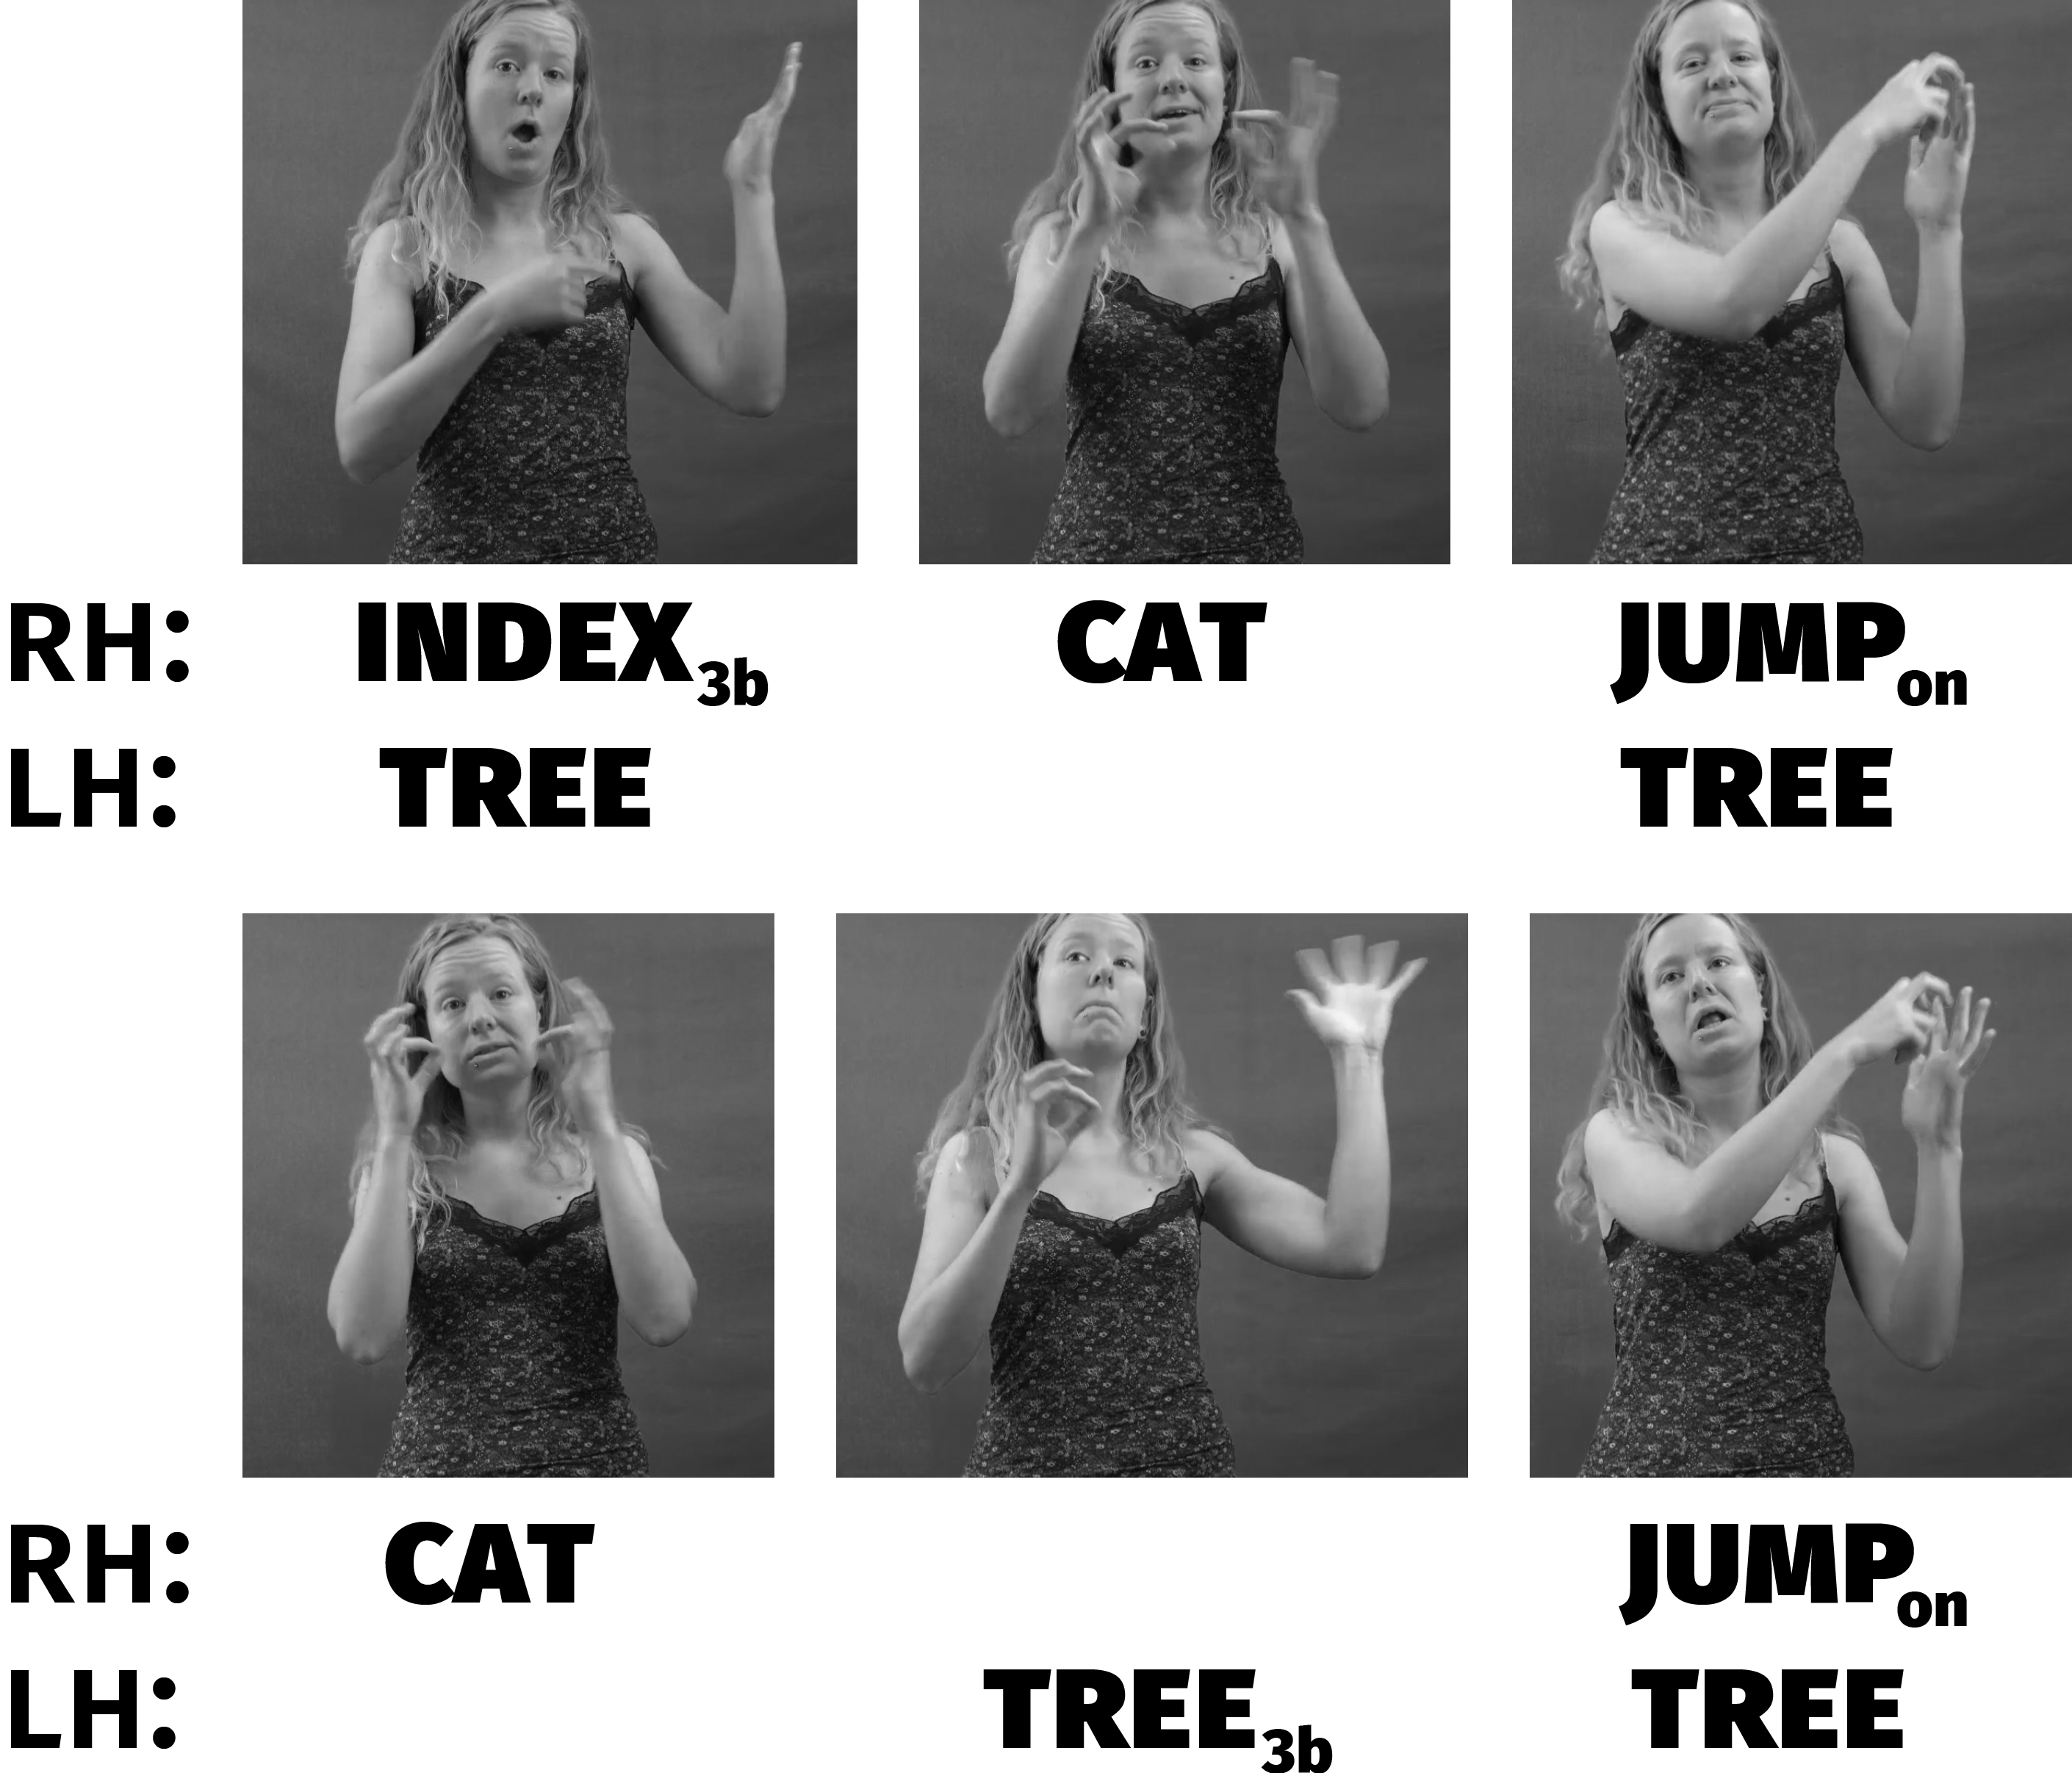
\includegraphics[width=.72\textwidth]{figuregroundcatsw.jpg}
	\caption{There are two options for expressing locative sentences in DGS. The top example shows a sentence in which the ground was not introduced in the previous discourse. In the bottom example, the ground was already introduced. The abbreviations `LH' and `RH' stand for left hand and right hand, respectively.}
	\label{fig:figuregroundcat}
\end{figure}

\clearpage 
What is interesting about the sentences in Figure \ref{fig:figuregroundcat} is that the ground is introduced by an index sign in the ground-figure sentence (top example) while this index is missing in the SOV sentence on the bottom of the figure. One could either argue that the ground is introduced first (as in spoken languages) in examples of the first kind leading to a deviation in constituent order or that the order in examples of the first kind, in fact, does not deviate, but that sentences of this kind consist of two clauses: the first one being an existential clause (`There is a tree') and the second one being the locative sentence (`The cat jumped on it'). 

Taken together, the vast majority of declarative sentences in DGS that are not highlighted in some way follow a more or less strict SOV pattern. Next, I will discuss polar interrogative sentences. Again, I will briefly outline the situation for spoken languages (Section \ref{generalpolar}), followed by a discussion of polar questions in sign languages (Section \ref{polarintsign}), and finally, sketch and analyze the phenomenon in DGS (Section \ref{polarinterrogativesdgs}).

\largerpage
\section{Polar interrogative sentences}\label{polargeneralsectionlabel}
\is{yes/no questions|see{polar interrogatives}}
\is{polar interrogatives|(}
This section is concerned with polar interrogatives. Again, I will briefly describe the situation in spoken languages (Section \ref{generalpolar}), the situation in sign languages (Section \ref{polarintsign}), and then discuss and analyze the phenomenon in DGS (Section \ref{polarinterrogativesdgs}). From the spreading behavior of the non-manuals used in polar interrogatives in DGS and distributional facts of manual signs that are probably related to FocP and IntP, I will discuss two modeling possibilities: either the  CP projection encoding interrogative force is right-headed or, alternatively, the projection is left-branching and the lexical material in polar interrogatives moves to this projection for feature-checking purposes. % the higher CP area encoding interrogative force are right-headed.


\subsection{General overview}\label{generalpolar}

\subsubsection{General introduction}
Polar interrogatives are sentences that are typically used to ask yes/no questions, i.e., questions that can be answered with `yes' or `no'. Cross-linguistically, there is much variation concerning the marking involved in polar interrogatives. Many, but not all languages use a special intonational contour (mainly rising final intonation), an initial or final question particle, special verb morphology, or a change in word order (\citealt[181--182]{sadock1985speech}; \citealt{dryer2013questions}). 

In the following, I will exemplarily discuss two strategies for expressing interrogative sentences in spoken languages and how they were analyzed. First, I will outline polar question formation in English and then discuss the same sentence type in the \is{Gungbe}\is{Gbe}Gungbe language Gbe. Although the strategies used in both languages are superficially very dissimilar, both languages were analyzed as involving an interrogative feature in the left periphery.

\subsubsection{Polar interrogatives in English}

In English, we find intonational marking as well as a change in word order. To be more precise, we find a rising intonation and subject-auxiliary inversion. This is shown in (\ref{simpleenglishpolarinterr}).

\begin{exe}
\ex\label{simpleenglishpolarinterr}\begin{xlist}
\ex Daniel will visit his neighbor. \hfill Declarative\label{simpleenglishpolarinterraaaa}
\ex Will Daniel visit his neighbor? \hfill Polar interrogative\label{simpleenglishpolarinterrbbbb}
\end{xlist}
\end{exe} 

\noindent English declaratives exhibit the order subject--auxiliary--verb, as illustrated in (\ref{simpleenglishpolarinterraaaa}). In polar interrogatives (\ref{simpleenglishpolarinterrbbbb}), the auxiliary \textit{will} raises into a higher position than the subject \textit{Daniel}. The same pattern is found in examples without auxiliaries. To do this, English makes use of \textit{do}-support, as illustrated in (\ref{simpleenglishpolarinterrtwo}).

\begin{exe}
\ex\label{simpleenglishpolarinterrtwo}\begin{xlist}
\ex Daniel visits his neighbor. \hfill Declarative\label{simpleenglishpolarinterra}
\ex Does Daniel visit his neighbor? \hfill Polar interrogative\label{simpleenglishpolarinterrb}
\end{xlist}
\end{exe} 

\noindent Standard analyses of English polar interrogatives assume that the purpose of the insertion (or the movement) of the auxiliary into a higher position is feature checking. \citet{roberts1993}, for example, assumes that the CP hosts a null question operator in English that triggers this kind of movement. Evidence for this comes, for example, from the fact that when an overt complementizer introducing a polar interrogative is present, as is the case in embedded questions, verb movement is blocked. This is illustrated in (\ref{englishembeddedquestions}).%Evidence for this comes %from different sources. I will just briefly sketch two of these sources.

\begin{exe}
\ex\label{englishembeddedquestions}\begin{xlist}
\ex \textcolor{white}{*}Bill asks whether Maria will come. \label{englishembeddedquestionsa}
\ex *Bill asks whether will Maria come.  \label{englishembeddedquestionsb}
\end{xlist}
\end{exe} 

\noindent Assuming that \textit{whether} is located in C\textdegree , we can assume that the auxiliary moves into exactly this position as it is not possible for the auxiliary to be hosted there when the position is taken by complementizers like \textit{whether} or \textit{if}.

The general assumption is that C\textdegree\ inherits a question feature or a question operator $[$Q$]$ that triggers subject-auxiliary inversion in root questions and that in embedded questions this feature is associated with a complementizer. For some researchers, most prominently \citet{cheng1997typology}, the movement of the auxiliary into C\textdegree\ is the crucial operation in clause-typing. 

\subsubsection{Polar interrogatives in Gbe}
In general, however, it should be stated that the processes underlying polar interrogatives are not well understood -- at least from a cross-linguistic perspective. This becomes obvious from the fact that there are many different mechanisms in the languages of the world that starkly differ from English (in fact, the subject-auxiliary inversion employed in English seems to be cross-linguistically a non-standard mechanism for marking polar questions, see \citealt{ultan1978some}). One such example are languages with clause-final question particles or languages with clause-final tonal question markers.

An example of the latter case is the Gbe language \is{Gungbe}Gungbe\label{gungbepolar} spoken in Benin. In this language, the difference between a declarative and a polar interrogative is marked by a clause-final floating low tone as illustrated by the minimal pair from \citet[93]{aboh2010sa}.\footnote{Tonal contours are indicated by accents. An acute (e.g. \textit{á}) represents a high tone, a grave (e.g. \textit{à}) a low tone, and a circumflex (e.g. \textit{\^{a}}) a high-low sequence.}

\begin{exe}
\ex Gunbe\label{yesnoquestiongungbe}
\begin{xlist}
\ex \gll {\textit{Sɛ́tɔ̀}} {\textit{kò}} {\textit{wá?}} \\
{Seto} {already} {come}\\
\trans `Seto arrived already.' \label{yesnoquestiongungbea} \hfill Declarative
\ex {\gll {\textit{Sɛ́tɔ̀}} {\textit{kò}} {\textit{w\^{a}?}} \\
{Seto} {already} {come.\textsc{inter}} \\
\trans `Has Seto arrived yet?' \label{yesnoquestiongungbeb} \hfill Polar question}
\end{xlist}
\end{exe}

\noindent The difference between a \is{Gungbe}Gungbe declarative and a Gungbe polar interrogative is, as the examples illustrate, the floating low tone only present in polar interrogatives (in the example, on \textit{w\^{a}}). In embedded polar questions both the floating low tone and an interrogative complementizer (an equivalent of English \textit{whether}) are present, as shown in the minimal pair in (\ref{yesnoquestiongungbetwo}), again from \citet[93]{aboh2010sa}.

\begin{exe}
\ex Gungbe\label{yesnoquestiongungbetwo}\begin{xlist}
\ex {\gll {\textit{Ùn}} {\textit{sè}} {\textit{ɖɔ̀}  } {\textit{Sɛ́tɔ}̀} {\textit{kò}} {\textit{wá?}} \\
{1\textsc{sg}} {hear} {that} {Seto} {already} {come} \\
\trans `I heard that Seto has already arrived.' \label{yesnoquestiongungbetwoa} \hfill Embedded declarative}
\ex {\gll {\textit{Ùn}} {\textit{kànbíɔ̀}} {\textit{ní}} {\textit{Sɛ́tɔ}̀} {\textit{kò}} {\textit{w\^{a}?}} \\
{1\textsc{sg}} {ask} {if} {Seto} {already} {come.\textsc{inter}} \\
\trans `I asked if Seto has already arrived.' \label{yesnoquestiongungbetwob} \hfill Embedded polar question}
\end{xlist}
\end{exe}

\noindent Other Gbe languages exhibit clause-final question particles and other structurally high categories, such as encoding the speaker's point of view, are also realized as clause-final heads \citep[211--213]{lefebvre2006creole}. Following \citeauthor{kayne1994antisymmetry}'s (\citeyear{kayne1994antisymmetry}) idea that heads always precede their complements, \citet{aboh2004morphosyntax} and  \citet{aboh2004left} argue that the interrogative feature, labeled $[+$interrogative$]$ here, located in the head of a (left-headed) interrogative phrase (IntP) attracts the whole proposition in a Gungbe\is{Gungbe}\is{Gbe} polar interrogative into its specifier. This is illustrated, in a slightly simplified version, in the tree in (\ref{ex:gungbepolarinterrogativetree}).

%\begin{exe}
%\ex\label{ex:gungbepolarinterrogativetree} 
%\begin{adjustbox}{width=\linewidth}
%\begin{tikzpicture}[baseline=(current bounding box.north), scale=0.80]
%\tikzset{level distance=35pt,sibling distance=5pt,every tree node/.style={align=center,anchor=north}}
%\Tree [.ForceP [.{SpecForceP} ] [.{$\overline{\textrm{Force}}$} [.{Force\textdegree } ] [.InterP [.SpecInterP \edge[roof]; \node(sleepyman){S\'{ɛ}t\`{ɔ} kò w\^{a}?}; ] [.{$\overline{\textrm{Inter}}$} [.{Inter\textdegree } {$[+$interrogative$]$} ] [.TopP [.SpecTopP ] [.{$\overline{\textrm{Top}}$} [.{Topic\textdegree } ] [.FocP [.SpecFocP ] [.{$\overline{\textrm{Foc}}$} [.{Foc\textdegree } ] [.IP \edge[roof]; \node(t){\qquad \textit{t} \qquad}; ] ] ] ] ] ] ] ] ]
%\draw[semithick,->] (t)..controls +(south west:4) and +(south:2)..(sleepyman);
%
%\end{tikzpicture}
%\end{adjustbox}
%\end{exe}

\begin{exe}
\ex\label{ex:gungbepolarinterrogativetree} 
\begin{forest}
for tree={s sep=5mm, inner sep=0, l=1mm} %s sep = Breite; l = Höhe
[ForceP [{SpecForceP} ] [{$\overline{\textrm{Force}}$} [{Force\textdegree } ] [InterP [SpecInterP [{S\'{ɛ}t\`{ɔ} kò w\^{a}?}, roof, name=sleepyman]] [{$\overline{\textrm{Inter}}$} [{Inter\textdegree } [{$[+$interrogative$]$}] ] [TopP [SpecTopP ] [{$\overline{\textrm{Top}}$} [{Topic\textdegree } ] [FocP [SpecFocP ] [{$\overline{\textrm{Foc}}$} [{Foc\textdegree } ] [IP [{\phantom{NNN}\textit{t}\phantom{NNN}}, roof, name=t] ] ] ] ] ] ] ] ] ]
%\draw[semithick,->] (t)..controls +(southwest:-4) and +(south:0.1)..(sleepyman);
\draw[->] (t) to[out=south west,in=south] (sleepyman);
%[CP[C][IP[I][VP[V][NP]]]]
\end{forest}
\end{exe}

%%%%%%%%%%%%%%%%%%%
%\clearpage
%%%%%%%%%%%%%%%%%%%

\noindent The tree shows a derivation of the simple polar question in (\ref{yesnoquestiongungbeb})\is{Gungbe} -- for a better orientation, I included the force, the topic and the focus projection. Evidence that such a phrasal movement analysis is plausible comes from topic and focus marking (and the fact that complementizers dominate embedded questions in the expected way (\ref{yesnoquestiongungbetwo}), where the complementizer would be located in the Force\textdegree\ in the tree). \citet{aboh2004left} shows that Gungbe has overt topic and focus markers which have to appear in a fixed order. Additionally, the topic and the focus markers appear in the expected clause-initial positions. An illustrative example of a topic and focus marker in an embedded clause is shown in (\ref{topicfocusmarkergungbe}).

\begin{exe}
\ex Gungbe \citep[168]{aboh2004left} \\ {\gll {\textit{Ùn}} {\textit{ɖɔ̀}} {\textit{ɖɔ̀}} {\textit{làn}} {\textit{l}ɔ̀} {yà} {\textit{Kòfí}} {\textit{wɛ́}} {\textit{Àsíbá}} {\textit{ní}} {\textit{ɖ}\textit{àɛ}} {\textit{n\'{a}}}  \\
{1\textsc{sg}} {say} {that} {meat} {\textsc{det}} {\textsc{top}} {Kofi} {\textsc{foc}} {Asiba} {\textsc{inj}} {cook.\textsc{3sg}} {for} \\
\trans `I said that, as for the meat Asiba should cook it for \textsc{Kofi}.' \label{topicfocusmarkergungbe} }
\end{exe}

\noindent The example in (\ref{topicfocusmarkergungbe}) shows that Gungbe has a topic and a focus marker in the left periphery that we can assume to be the heads of the corresponding projections. As predicted by \citeauthor{rizzi1997fine}'s (\citeyear{rizzi1997fine}) split-CP model, the order of these particles strictly has to be \textit{yà}--\textit{wɛ́}, while the opposite order, *\textit{wɛ́}--\textit{yà} is ungrammatical (i.e., the topic marker has to precede the focus marker). Interestingly, when a Gungbe interrogative sentence is embedded, the embedded sentence is sandwiched between the complementizer and the interrogative particle. However, in the case of an embedded polar interrogative, the topic and the focus marker are reversed, as shown in (\ref{topicfocusmarkergungbetwo}), and occur in a clause-final position. 

\begin{exe}
\ex Gungbe \citep[184]{aboh2004left} \\ {\gll {\textit{Ùn}} {\textit{kànb'{i}'{ɔ}}} {\textit{ɖɔ̀}} {\textit{Kòfí}} {\textit{ní}} {\textit{xɔ̀}} {\textit{mótò}} {\textit{wɛ́}} {\textit{y\textdoublegrave{a}}}  \\
{1\textsc{sg}} {ask} {that} {Kofi} {\textsc{inj}} {buy} {car} {foc} {top-inter}  \\
\trans `I asked whether \textsc{Kofi should buy a car} $[$as planned/mentioned$]$.' \label{topicfocusmarkergungbetwo} }
\end{exe}


\noindent As can be seen from (\ref{topicfocusmarkergungbetwo}),\is{Gungbe} the embedded clause is sandwiched in between the complementizer in Force\textdegree\ and the topic, focus, and interrogative marker. This order is derived by moving the chunk to be focused (the translational equivalent of \textit{Kofi should buy a car}) into the specifier of the focus projection. Then the whole focus projection, together with the focus particle, is moved into the specifier of the topic position. Finally, the TopP is, together with the topic particle, moved into the specifier of the IntP \citep[184]{aboh2004left}. This not only derives the correct order, but supports the idea that Gungbe makes massive use of phrasal movement into specifier positions.

Taken together, the discussion of English and Gungbe\is{Gungbe}\is{English} has shown that languages may make use of very different strategies to express polar interrogative sentence. However, despite their surface differences, the data can be accounted for by assuming that an interrogative head exists in the CP system that needs to be checked in some way.

\subsection{Polar interrogatives in sign languages}\label{polarintsign}



%Syntactic structure
\subsubsection{General introduction}
While some spoken languages make use of a change in word order to mark polar interrogatives, this strategy was, so far, not reported for any sign language. Instead, polar interrogatives use the same word order as declaratives with the addition of a special non-manual marking that usually accompanies the whole clause. An example of this kind of language is \is{Croatian Sign Language}Croatian Sign Language. In this language, a polar question is formed without a change in word order but with the addition of a combination of non-manual markers. This is shown in (\ref{polarcroation}) from \citet[157]{sarac2006interrogative}.

\begin{exe}
\ex Croatian Sign Language\label{polarcroation}\begin{xlist}
\ex \textsc{man sleep}
\glt `The man is sleeping.' \label{polarcroationa} 
\ex \slg[polar-q]{man sleep}
%{\hspace{23pt}polar-q}  \\
%{$\overline{\textrm{\textsc{man sleep}}}$} %\\
\glt `Is the man sleeping?' \label{polarcroationb} 
\end{xlist}
\end{exe}


\noindent The example illustrates that a sentence without the non-manuals labeled `polar-q' is interpreted as a statement (\ref{polarcroationa}). Adding the non-manuals leads to a polar-question interpretation (\ref{polarcroationb}). In fact, this strategy is the most wide-spread way to form a polar question across the sign languages of the world.

In the following, I will first describe the non-manuals used in polar questions across different sign languages and the use of question particles. Then I will briefly review two exemplary syntactic accounts on polar interrogatives in sign languages. One account by \citet{sarac2006interrogative} and one by \citet{aboh2010sa} -- in both accounts, the formation of polar interrogatives in sign languages involves XP movement.

\subsubsection{Non-manual markers}
All\label{nnmpolarintsign} sign languages studied so far use non-manual markers for polar interrogatives. Interestingly, the non-manuals employed for this type of interrogative seems to be cross-linguistically very stable. \citet[19]{zeshan2004interrogative}, in her typological study on thirty-five geographically and genetically diverse sign languages lists the following non-manual markers that were used for polar interrogatives in her sample:

\newpage 
\begin{itemize}[itemsep=0pt]
	\item eyebrow raise
	\item eyes wide open
	\item eye contact with the addressee
	\item head forward position
	\item forward body posture
\end{itemize}

\noindent Usually, one of these non-manual markers or a combination of several non-man\-uals is employed, spreading over the whole clause as, for example, in \is{American Sign Language}American Sign Language (cf. \citealt{wilbur1999syntactic}). Additionally, one or several non-manuals may have a different spreading domain (for example, eyebrow raise spreading over the whole clause, but the head is put forward only on the lexical material at the end of the clause). In most sign languages, eyebrow raise seems to be the main marker of polar interrogatives spreading over the whole clause. For some sign languages, however, it is reported that they use chin down and/or head forward as their main marker of polar interrogatives. Examples include \is{Croatian Sign Language}Croatian Sign Language and \is{Turkish Sign Language}Turkish Sign Language. In both languages, however, polar interrogatives are also accompanied by a raising of the brows (e.g., \citealt{sarac2006interrogative}).

A hard-to-answer question is whether there is one particular marker in a sign language for clause-typing a polar interrogative or if it is a combination. Put differently: there is often a bundle of several non-manuals involved in fulfilling one function (here: marking a clause as being a polar interrogative).

One solution to the puzzle that we usually find more than one non-manual marker involved in (polar) interrogatives could be that each marker contributes a different function -- all related to polar interrogatives. The idea that non-manuals combine in a compositional way is indeed attractive (e.g., \citealt{nespor1999prosody, sandler2006sign, dachkovsky2009visual, herrmann2013modal}).\footnote{\citet{dachkovsky2009visual}, for example, show that conditional sentences in \is{Israeli Sign Language}Israeli Sign Language are marked by brow-raise. This non-manual marker can also be found with counterfactuals, but with an additional squint. They argue that both non-manuals have general meanings that combine compositionally in Israeli Sign Language.} If one looks at what constitutes a question, several sub-functions can be identified. \citet[4]{dayal2016questions}, for example, lists the following conditions that must be met in order to talk about a real information-seeking question:

\begin{enumerate}[itemsep=0pt]
	\item The speaker/signer does not know the truth about the proposition embedded in the question.
	\item The speaker/signer wants to know the truth about the proposition embedded in the question.
	\item The speaker/signer believes that the interlocutor being asked knows the truth about the proposition embedded in the question.
\end{enumerate}


\noindent It may well be that each of these functions can be grammaticalized as a non-manual marker in a sign language (and additionally, it is possible that one sign language grammaticalizes one function and another sign language another function). The idea that non-manual markers compositionally combine in polar interrogatives will be explored for German Sign Language later. Next, I will briefly discuss the use of question particles in polar interrogatives.

\subsubsection{Question particles}
Some sign languages make use of specialized interrogative particles (next to non-manual markers) to mark polar interrogatives that mainly occur clause-finally and sometimes clause-initially. It has to be stressed, however, that in all sign languages that employ question particles the use of non-manual markers is still obligatory \citep[21]{zeshan2004interrogative}. This is in line with older observations. \citet{liddell1977non}, for example, reports that the manual question particle that is used in \is{American Sign Language}American Sign Language does not substitute non-manual markings in polar interrogatives. However, the behavior of non-manuals in polar interrogatives with a question particle is subject to cross-linguistic variation. The question particle in American Sign Language, for example, is obligatorily used with non-manual markings that accompany the particle and may optionally spread over the  whole clause \citep[122--124]{neidle2000syntax}. Another sign language that was reported to have a question particle is \is{Hong Kong Sign Language}Hong Kong Sign Language \citep[206]{tang2006questions}. In this sign language, the non-manuals only accompany the question particle and do not spread. 

\subsubsection{Syntactic analysis I: \citet{sarac2006interrogative}}
Most syntactic theories addressing polar interrogatives in sign languages assume some kind of phrasal movement. \citet{sarac2006interrogative} are concerned with polar interrogatives in \is{Croatian Sign Language}Croatian Sign Language (cf. the example in (\ref{polarcroationb})). 
As the intensity of the non-manuals increases towards the end of such polar questions, \citet{sarac2006interrogative} assume that their source is to be located at the right edge of the clause (cf. the Non-Manuals as Syntactic Markers Hypothesis discussed on page \pageref{nmasmh}). This source is assumed to be C\textdegree . For receiving a question then, the lexical material has to be moved from the IP to SpecCP in order to check an interrogative feature. Feature checking (or spec-head agreement) in this case leads to the non-manual marking: ``This material $[$i.e., the material in SpecCP$]$ carries the non-manual material associated with $[$Q$]$'' \citep[222]{sarac2006interrogative}. This is illustrated in (\ref{ex:petroniolillomartinleftwardababa}).


\begin{exe}
\ex\label{ex:petroniolillomartinleftwardababa} 
\begin{forest}
for tree={s sep=25mm, inner sep=0, l=20mm} %s sep = Breite; l = Höhe
%[CP [SpecCP[{\slg[pol]{man sleep}},roof]][{$\overline{\textrm{C}}$}[IP[{\phantom{NNN}\textit{t}\phantom{NNN}},roof]][C [$\lbrack+$Q$\rbrack$]]]]
[CP [SpecCP [{\slg[pol]{man sleep}},roof,name=sleepyman] ] [{$\overline{\textrm{C}}$} [IP [ {\phantom{NNN}\textit{t}\phantom{NNN}},roof,name=t ]  ] [C [{$\lbrack+$Q$\rbrack$}] ] ] ]
%[CP[C][IP[I][VP[V][NP]]]]
\draw[semithick,->] (t)..controls +(south west:3) and +(south:1)..(sleepyman);
\end{forest}
\end{exe}

%\begin{tikzpicture}[baseline]
%\tikzset{level distance=30pt,sibling distance=45pt,every tree node/.style={align=center,anchor=north}}
%\Tree [.CP [.SpecCP \edge[roof]; \node(sleepyman){\slg[pol]{man sleep}}; ] [.{$\overline{\textrm{C}}$} [.IP \edge[roof]; \node(t){\qquad \textit{t} \qquad}; ] [.C {$[$+Q$]$} ] ] ]
%\draw[semithick,->] (t)..controls +(south west:3) and +(south:1)..(sleepyman);
%\end{tikzpicture}
%\end{exe}

%\begin{exe}
%\ex\label{ex:petroniolillomartinleftwardababa} 
%\begin{tikzpicture}[baseline]
%\tikzset{level distance=30pt,sibling distance=45pt,every tree node/.style={align=center,anchor=north}}
%\Tree [.CP [.SpecCP \edge[roof]; \node(sleepyman){\slg[pol]{man sleep}}; ] [.{$\overline{\textrm{C}}$} [.IP \edge[roof]; \node(t){\qquad \textit{t} \qquad}; ] [.C {$[$+Q$]$} ] ] ]
%\draw[semithick,->] (t)..controls +(south west:3) and +(south:1)..(sleepyman);
%\end{tikzpicture}
%\end{exe}

%\vspace{-0.3cm}

\noindent Based on \citeauthor{sarac2006interrogative}'s (\citeyear{sarac2006interrogative}) account, declaratives and polar interrogatives only have the same structure superficially (see also \citealt{sarac2007cross}). The latter are, however, the result of the IP being moved to (or being remerged in) SpecCP.

\subsubsection{Syntactic analysis II: \citet{aboh2010sa}}
Finally, I will briefly discuss an idea developed by \citet{aboh2010sa} for (\textit{inter alia}) \is{Sign Language of the Netherlands}Sign Language of the Netherlands. Their account is similar to what has been proposed for polar interrogatives in \is{Gungbe}Gungbe (see page \pageref{ex:gungbepolarinterrogativetree}). Although they mainly discuss constituent interrogatives, they propose that Sign Language of the Netherlands has an optional clause-final question particle consisting of the hands being open with palms facing upwards. This sign is usually called `palm-up gesture' (\textsc{p-ug} for short). On their account, \textsc{p-ug} is located in the head of the IntP. 

As their account is strictly antisymmetric, all heads are left-headed and all specifiers are left-branching. As \textsc{p-ug} appears clause-final, they assume that the material located in the IP is obligatorily moved into the specifier of the IntP in polar interrogatives. This not only derives the correct surface order with \textsc{p-ug} in a clause-final position but also accounts for the fact that the non-manuals are strongest clause-finally as all manual material is then to the left of the Int\textdegree\ that we can easily assume to be the trigger of the non-manual markings.

The difference between the two models is simply that \citet{sarac2006interrogative} assume a right- and \citet{aboh2010sa} a left-headed structure. Under the assumption that the respective head is the trigger of the non-manuals, both models account for the spread of the non-manuals with a clause-final intensity peak.

\subsection{Polar interrogatives in DGS}\label{polarinterrogativesdgs}
In this section, I will first discuss the non-manual markings and their spreading behavior in DGS polar interrogatives and then discuss the use of the palm-up gesture (\textsc{p-ug}) and the behavior of pronoun doubling. I follow earlier proposals that \textsc{p-ug} is located in the head of the IntP \citep{aboh2010sa} and the pronoun double in the head of the FocP \citep{de1999phrase} and show that their order as well as the spreading behavior of the non-manuals can be derived by assuming a right-headed or left-headed account.

\subsubsection{Non-manual markings}
As with other sign languages, the constituent-order in polar interrogatives in DGS is not different from declarative sentences and is thus SOV. The only difference between a declarative and a polar interrogative sentence lies in non-manual marking. With polar questions, signers raise their eyebrows. Additionally, the head is often put forward and tilted (see also \citealt[171--172]{papaspyrou2008grammatik}). While the raising of the eyebrows obligatorily spreads over the whole clause, the forward-stretch of the head as well as the tilting only occurs on the clause-final sign, in most cases on the verb. This demonstrated in Figure \ref{fig:polarint}. The peak of the non-manual markings on the whole can be observed towards the end of the clause.

\begin{figure}[bt]
\centering
	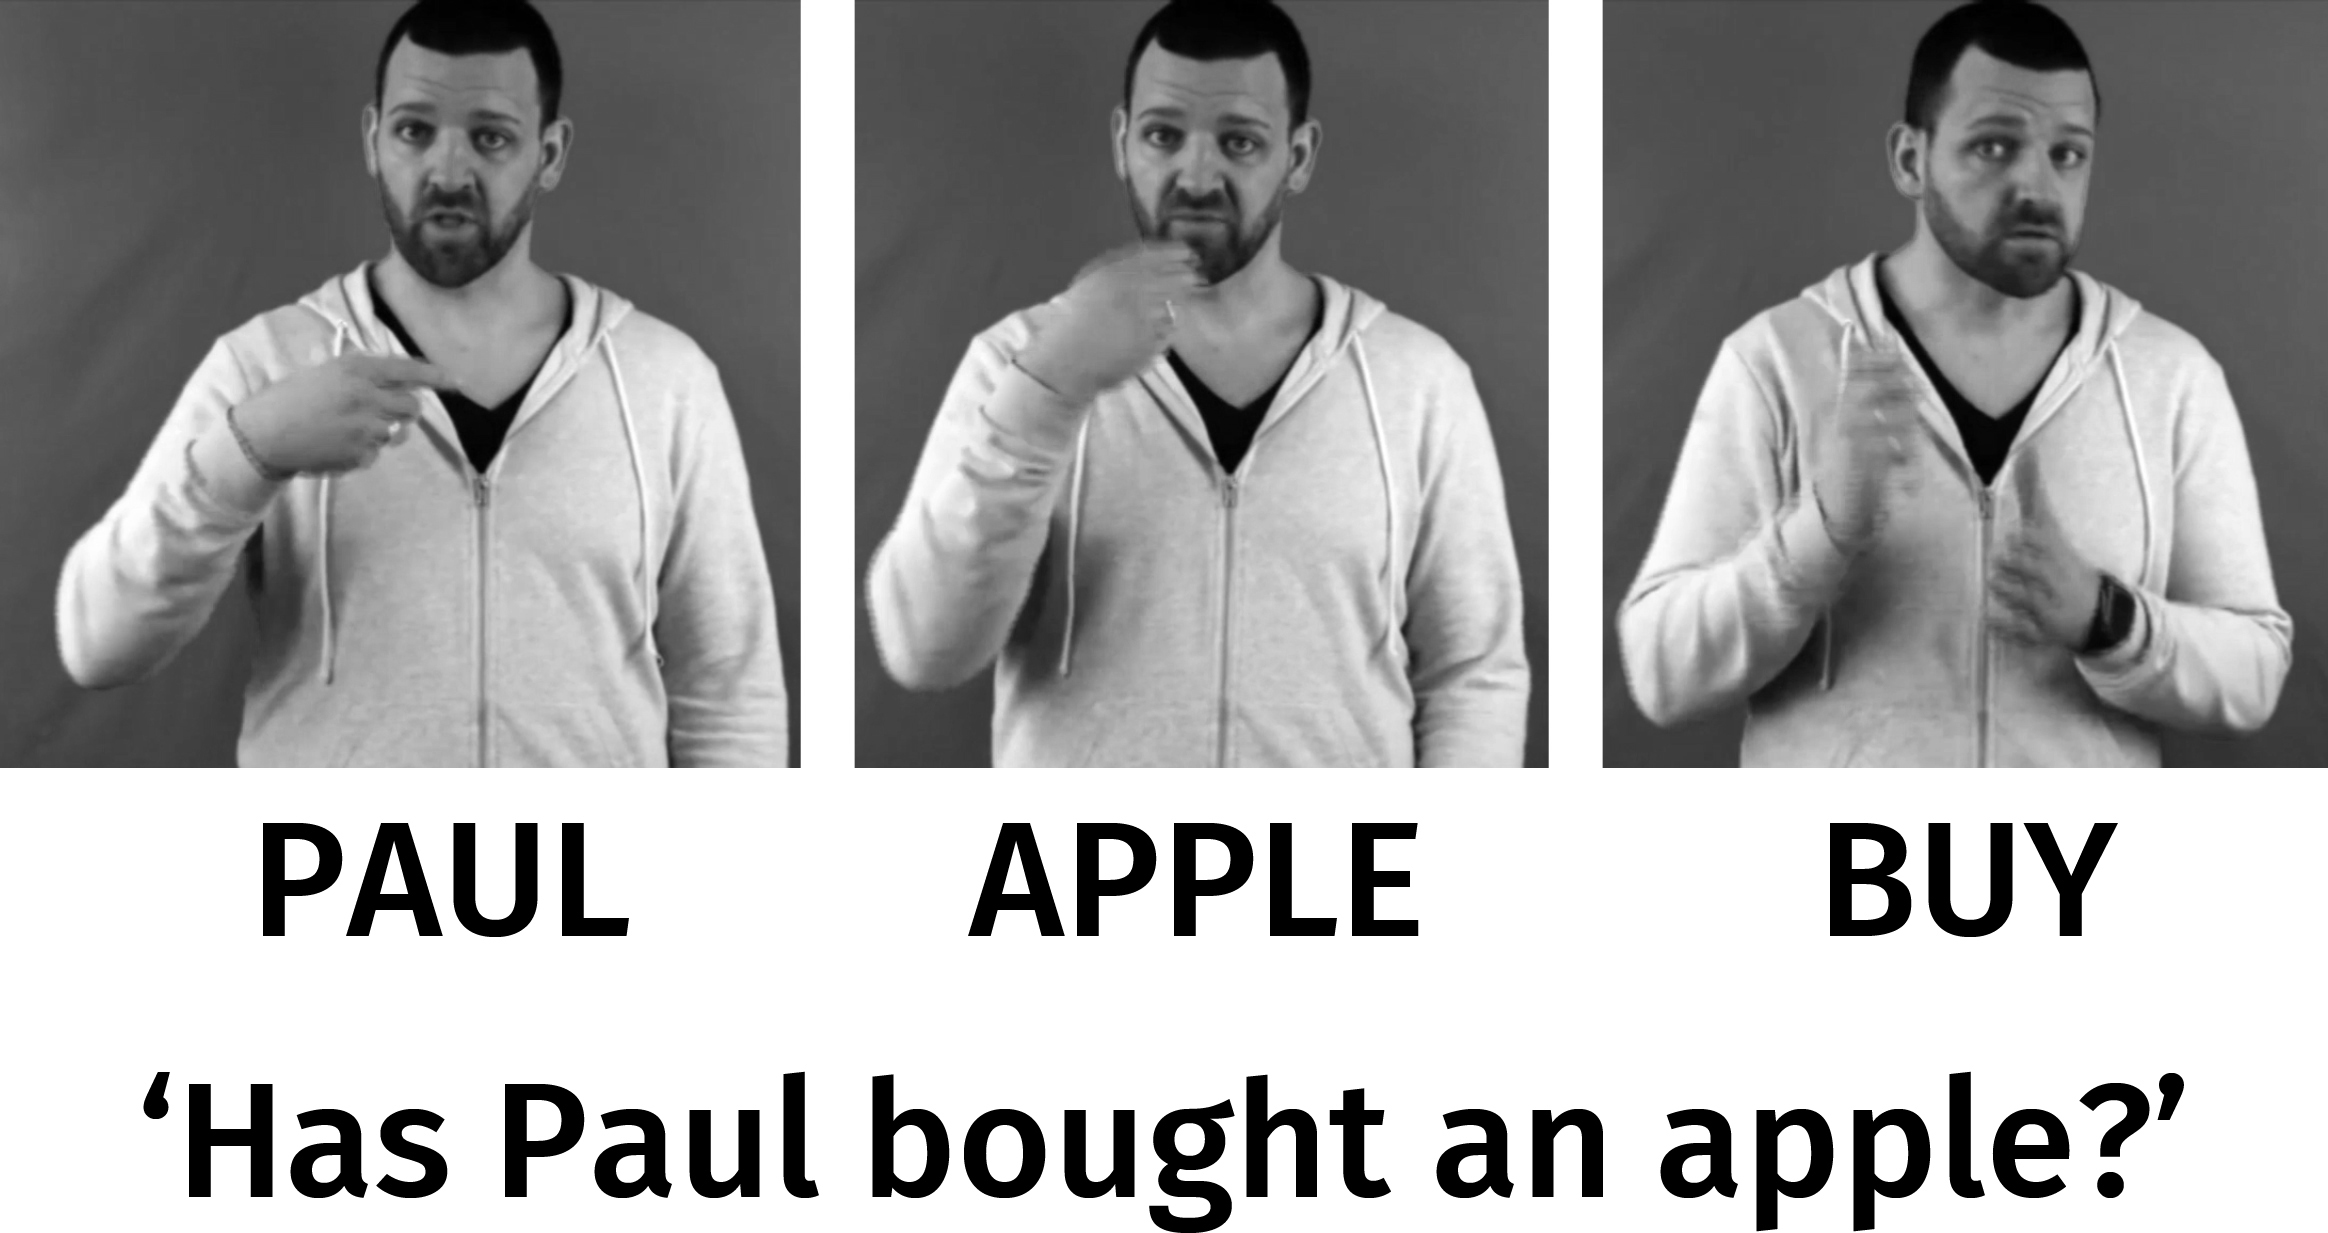
\includegraphics[width=1.0\textwidth]{yesnoquestionsw.jpg}
	\caption{The non-manuals used in DGS polar interrogatives: raised eyebrows obligatorily spread over the whole clause. Additionally, the clause-final sign is often accompanied by a forward movement of the head and a tilt.}
	\label{fig:polarint}
\end{figure}

Each of the three non-manuals, raising the eyebrows, putting the head forward, and tilting it, fulfills a separate function. While raising the eyebrows is obligatory, the forward movement and the tilt can sometimes be absent. As the brow raise is obligatory, I will take it to be the main non-manual marker responsible for clause-typing. Putting the head forward indicates that the signer awaits a response \citep[171--172]{papaspyrou2008grammatik}. Finally, the head tilt indicates epistemic commitment: the more the head is tilted, the lower the signer's epistemic commitment. In other words: the more the head is put sideways, the more insecure the signer is about the proposition expressed. This explains why it is absent in utterances that only have the surface form of a polar question, such as rhetorical or inclination questions. This is illustrated in Figure \ref{fig:epistemiccommitment} which shows the non-manuals used in a polar question with low epistemic commitment (on the left a screenshot from the question \textit{Can I do an apprenticeship?}) and an inclination question with high epistemic commitment (on the right a screenshot from the question \textit{Can you pass me the salt?}). As the head tilt is not only found in polar interrogatives, but in general is an epistemicity marker, I will discuss it later (see Section \ref{perhapsmoodirrealis} and \ref{rhetq}). Taken together, the three non-manual markers in DGS each fulfill a separate function and can thus be analyzed compositionally.

\begin{figure}[bt]
\centering
	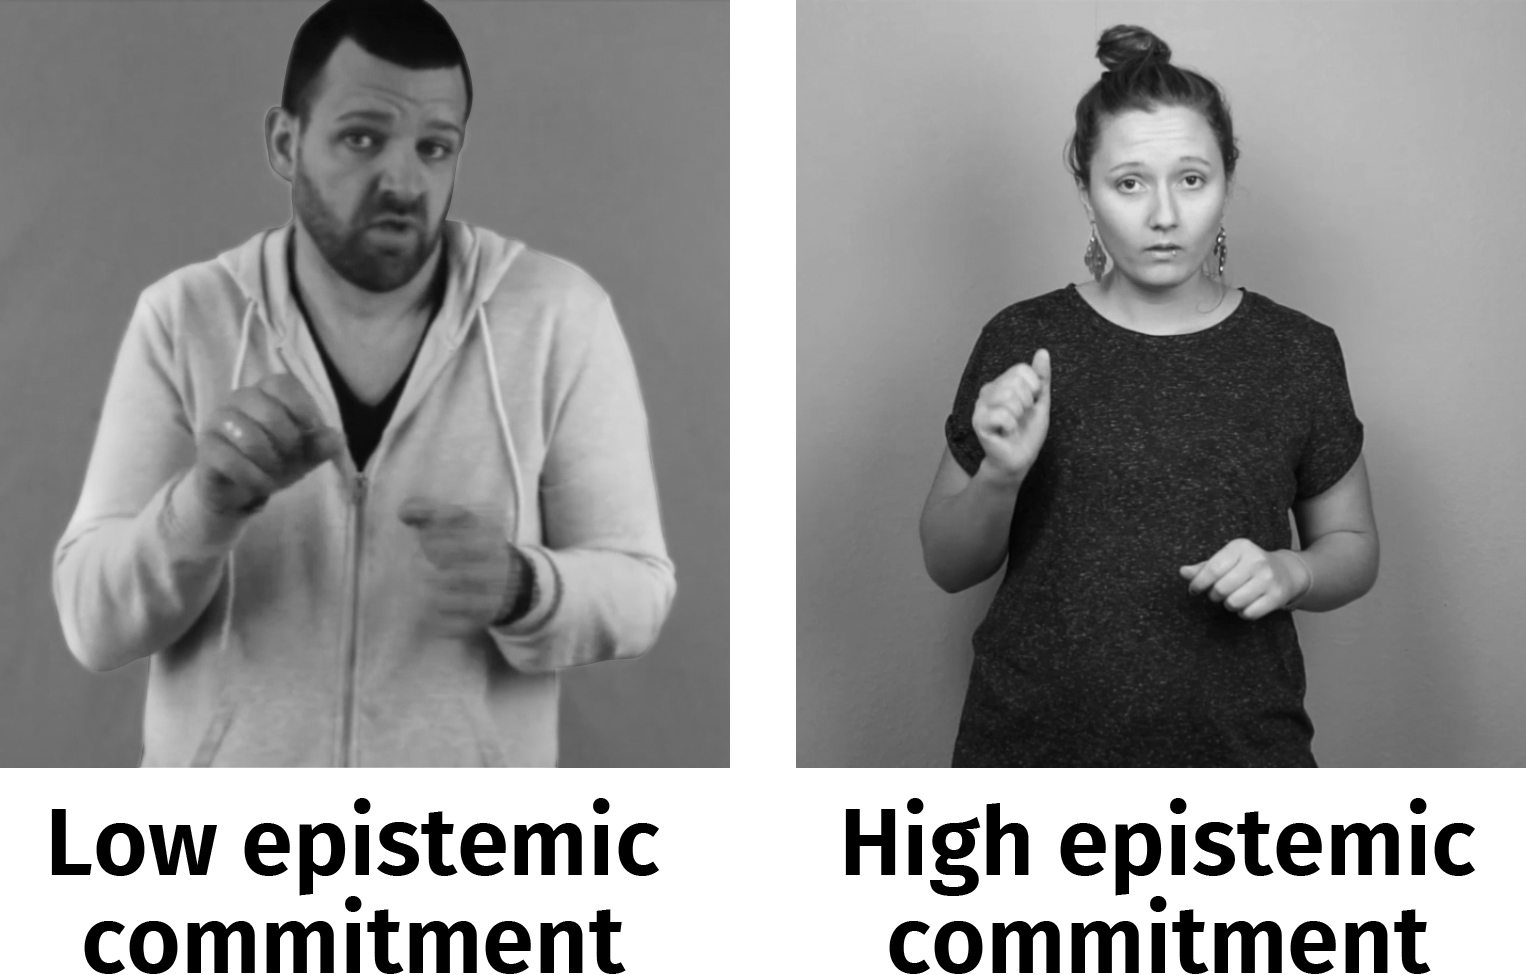
\includegraphics[width=.7\textwidth]{epistemiccommitmentsw.jpg}
	\caption{Non-manual markings used with polar interrogatives with low and high epistemic commitment. In both cases, the eyebrows are raised and the head is put forward. When the head is additionally tilted to the side as in the picture on the left, the signer signals that s/he is insecure about the proposition. When the head is held straight, in contrast, the signer is confident.}
		\label{fig:epistemiccommitment}
\end{figure}	

\largerpage
\subsubsection{Manual question markers and focus doubling: two possible syntactic analyses}\label{manualquestionmarkers}
That the non-manuals reach their maximum at the end of the clause (this is also true for the raised eyebrows) could be taken as evidence for a right-peripheral interrogative head or, alternatively, as evidence for the fact that the phrase structure below the IntP has moved in an Aboh-\&-Pfau-like manner into SpecIntP as discussed in the previous section for \is{Sign Language of the Netherlands}Sign Language of the Netherlands. Using distributional facts of focus and question particles, I will show that both options can be syntactically implemented. Before doing this, I will briefly discuss the use of question particles and focus marking in polar interrogatives in DGS.

Similar to what \citet{aboh2010sa} describe for Sign Language of the Netherlands, it is possible in DGS to make use of an optional clause-final question particle that is extremely similar to the one used in Sign Language of the Netherlands and is usually also glossed \textsc{p-ug}. Its use is illustrated in (\ref{pugpolarintdgs}).

\begin{exe}
\ex \slg[pol]{index\textsubscript{2} can cook p-ug}
%{\hspace{113pt}pol}  \\
%{$\overline{\textrm{\textsc{index}\textsubscript{2} \textsc{can cook p-ug}}}$} 
\glt `Can you cook?'\label{pugpolarintdgs}
\end{exe}

\noindent If \textsc{p-ug} is indeed located in the head of the IntP, the suggestion that all manual material located in the IP in DGS is moved to SpecIntP is a plausible scenario. Alternatively, one might hypothesize that the Int\textdegree\ is right-headed in DGS. 

\largerpage
The\is{focus doubling} same conclusions are to be drawn from the position of focus doubles in DGS. Polar interrogatives, together with imperatives, show a peculiar pattern of pronoun doubling in DGS. In many cases, polar questions with pronoun doubling are not unmarked polar questions. Instead, questions with doubled pronouns often receive emphasis, mainly to indicate that the speaker is surprised (however, this is not necessarily the case. Sometimes pronoun doubling also takes place in regular polar questions). This is illustrated in the following examples.

\vspace{-0.2cm}

\begin{exe}
\ex\label{unmarkedpolarvsdoubling}\begin{xlist}
\ex \slg[pol]{index\textsubscript{2} can cook}
%\ex {\hspace{81pt}pol}  \\
%{$\overline{\textrm{\textsc{index}\textsubscript{2} \textsc{can cook}}}$} %\\
\glt `Can you cook?' \label{ex:unmarkedpolarvsdoublinga}\hfill Regular polar question
\ex \slg[pol]{index_2 can cook \slg[foc]{index\textsubscript{2}}} 
%
%
%\glll   {${\hspace{104pt}\underline{\textrm{\textcolor{white}{lllllll}foc}}}$} \\
%{\hspace{123pt}pol} \\
%{$\overline{\textrm{\textsc{index}\textsubscript{2} \textsc{can cook index}\textsubscript{2}}}$} \\
\glt `YOU can cook?' \label{ex:unmarkedpolarvsdoublingb}\hfill Pronoun doubling

\end{xlist}
\end{exe}
 

\noindent Doubling as in (\ref{ex:unmarkedpolarvsdoublingb}) has generally been referred to as `focus doubling' in the literature. The term `focus doubling' is chosen as it is assumed that the clause-final double is located in a focus position, to be more precise in the head of a focus phrase as only heads, but not phrases, can be doubled (e.g., \citealt{de1999phrase, sandler2006sign}, but see \citealt{wilbur2012informationstructure} who argues that doubling does not serve as a focus, but as a marker of emphasis). This is in line with the idea that focus is located in a clause-final position in many sign languages (see \citealt{wilbur1991intonation, wilbur1994foregrounding, wilbur1996evidence, wilbur1997prosodic} for \is{American Sign Language}American Sign Language). Besides pronouns, other parts of speech can undergo doubling in DGS as well. This is, for example, true for \textit{wh}-signs or modals. 

If the focus double is in the head of FocP, the fact that it occurs clause-finally in DGS is, again, in line with the idea of the IP being moved to SpecIntP or a right-headed Foc\textdegree . Additionally, both modeling possibilities are in line with the fact that the intensity peak of the non-manuals is clause-final in DGS. If taken to the extremes (with all heads and specifiers on the same side), these two modeling possibilities look as depicted in (\ref{ex:polarquestionsanalyis}). 
%\vspace{-0.5cm}
%\clearpage
%\begin{exe}
%\ex\label{ex:polarquestionsanalyis}
%\begin{multicols}{2}
%\begin{xlist}
%
%\ex \label{ex:polarquestionsanalyisa}
%\begin{tikzpicture}[baseline=(current bounding box.north), scale=0.7]
%\tikzset{sibling distance=1pt}
%\tikzset{every tree node/.style={align=left,anchor=north}}
%\Tree [.IntP [.{$\overline{\textrm{Int}}$} [.FocP [.{$\overline{\textrm{Foc}}$} [.IP \edge[roof]; \node(t){\qquad\qquad}; ] [.{Foc\textdegree } ] ] [.SpecFocP ] ] [.{Int\textdegree } ] ] [.SpecIntP ] ]
%\end{tikzpicture}
%
%
%\ex\label{ex:polarquestionsanalyisb}
%\begin{tikzpicture}[baseline=(current bounding box.north), scale=0.7]
%\tikzset{sibling distance=1pt}
%\tikzset{every tree node/.style={align=left,anchor=north}}
%
%\Tree [.IntP [.SpecIntP \edge[roof]; \node(specintp){\textcolor{white}{blablabla}}; ] [.{$\overline{\textrm{Int}}$} [.{Int\textdegree } ] [.FocP [.SpecFocP ] [.{$\overline{\textrm{Foc}}$} [.{Foc\textdegree } ] [.IP \edge[roof]; \node(t){\qquad\qquad}; ] ] ] ] ]
%
%\draw[semithick,->] (t)..controls +(south west:4) and +(south:2)..(specintp);
%
%
%
%\end{tikzpicture}
%
%
%\end{xlist}
%\end{multicols}
%\end{exe}




\begin{exe}
\ex\label{ex:polarquestionsanalyis} 
\begin{xlist}

\ex \label{ex:polarquestionsanalyisa}
\begin{forest}
for tree={s sep=5mm, inner sep=0, l=12mm} %s sep = Breite; l = Höhe
[IntP [{$\overline{\textrm{Int}}$} [FocP [{$\overline{\textrm{Foc}}$} [IP [{\qquad\qquad}, roof] ] [{Foc\textdegree } ] ] [SpecFocP ] ] [{Int\textdegree } ] ] [.SpecIntP ] ]
%[CP[C][IP[I][VP[V][NP]]]]
\end{forest}


\ex\label{ex:polarquestionsanalyisb}

\begin{forest}
for tree={s sep=5mm, inner sep=0, l=12mm} %s sep = Breite; l = Höhe
[IntP [SpecIntP [{\textcolor{white}{blablabla}}, roof,name=specintp] ] [{$\overline{\textrm{Int}}$} [{Int\textdegree } ] [FocP [SpecFocP ] [{$\overline{\textrm{Foc}}$} [{Foc\textdegree } ] [IP [{\qquad\qquad}, roof, name=t] ] ] ] ] ]
\draw[semithick,->] (t)..controls +(south west:4) and +(south:2)..(specintp);
%[CP [SpecCP] [$\overline{\textrm{C}}$ [IP[SpecIP][$\overline{\textrm{I}}$[VP[SpecVP][$\overline{\textrm{V}}$[{\phantom{V}}][V\textdegree]]][I\textdegree]]][C\textdegree]]]
%%[CP[C][IP[I][VP[V][NP]]]]
\end{forest}
\end{xlist}
\end{exe}\vspace*{-1cm}

\noindent The structure on the left (\ref{ex:polarquestionsanalyisa}) allows specifiers and heads to the right, while the structure on the right (\ref{ex:polarquestionsanalyisb}) shows an anti-symmetric Aboh-\&-Pfau-style structure with all heads and specifiers to the left. To form a polar interrogative, we need to assume movement of the IP material into the specifier of the IntP in the right structure. The non-manuals would then be triggered by spec-head agreement. In the case that a focus double is present, we would assume that it is not only the IP, but the whole FocP that moves to SpecInt. For the model on the left, one would assume an active Int\textdegree\ triggering the non-manuals via c-command without additional movement to SpecInt. In both models, \textsc{p-ug} and focus doubles are predicted to be clause final.

However, the models differ in their prediction of how \textsc{p-ug} and the focus double are ordered. The Aboh-\&-Pfau-style structure predicts that the focus double follows \textsc{p-ug}, while the structure on the right predicts the opposite. What we find is that the question particle \textsc{p-ug} follows rather than precedes the pronoun double in DGS, as shown in (\ref{ex:doublingandpug}) and Figure (\ref{fig:beerbuyyou}).




\begin{exe}
\ex\label{ex:doublingandpug}\begin{xlist}
\ex \textcolor{white}{*}\slg[pol]{index_2 beer buy index_2 p-ug}
\glt \textcolor{white}{*}`Are \textsc{you} buying beer?' \label{ex:doublingandpuga}
\ex *\slg[pol]{index_2 beer buy p-ug index_2}
\glt \textcolor{white}{*}`Are \textsc{you} buying beer?' \label{ex:doublingandpugb}
\end{xlist}
\end{exe}

\noindent The model on the left in (\ref{ex:polarquestionsanalyis}) can derive a structure like the one in (\ref{ex:doublingandpuga}) as shown in the tree in (\ref{ex:polarquestionsanalyisaaba}).

\begin{figure}[t]
\centering
	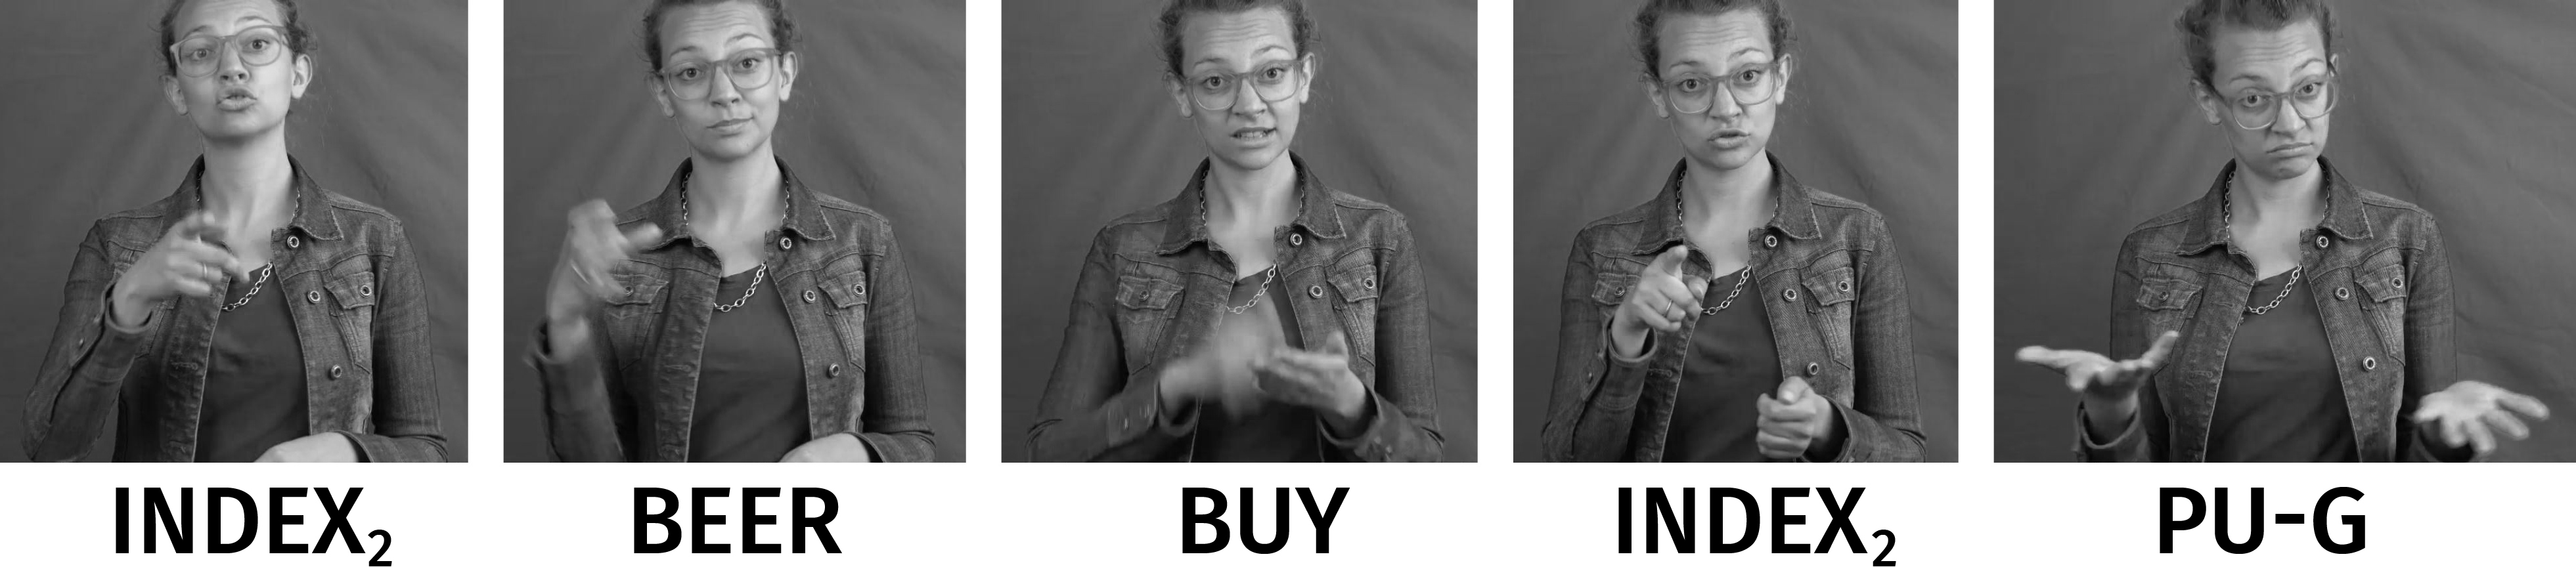
\includegraphics[width=1.0\textwidth]{beerbuyyousw.jpg}
	\caption{The palm-up gesture has to follow a focus double in DGS.}
	\label{fig:beerbuyyou}
\end{figure}

%\begin{exe}
%\ex \label{ex:polarquestionsanalyisaaba}
%\begin{tikzpicture}[baseline=(current bounding box.north), scale=1.00]
%\tikzset{sibling distance=1pt}
%\tikzset{every tree node/.style={align=left,anchor=north}}
%\Tree [.IntP [.{$\overline{\textrm{Int}}$} [.FocP [.{$\overline{\textrm{Foc}}$} [.IP \edge[roof]; \node(t){\textsc{index}\textsubscript{2} \textsc{beer buy}}; ] [.{Foc\textdegree } {\textsc{index}\textsubscript{2}} ] ] [.SpecFocP ] ] [.{Int\textdegree } {\textsc{p-ug}} ] ] [.SpecIntP ] ]
%\end{tikzpicture}
%
%\end{exe}

\begin{exe}
\ex \label{ex:polarquestionsanalyisaaba}
\begin{forest}
for tree={s sep=25mm, inner sep=0, l=12mm} %s sep = Breite; l = Höhe
[IntP [{$\overline{\textrm{Int}}$} [FocP [{$\overline{\textrm{Foc}}$} [IP [{\textsc{index}\textsubscript{2} \textsc{beer buy}},roof] ] [{Foc\textdegree } {\textsc{index}\textsubscript{2}} ] ] [SpecFocP ] ] [{Int\textdegree } {\textsc{p-ug}} ] ] [SpecIntP ] ]
%[CP[C][IP[I][VP[V][NP]]]]
\end{forest}

\end{exe}





\noindent While this model gets rid of the additional movement steps that would be needed in an anti-symmetric model, it is not impossible to derive the correct order in the latter. For this, we would assume that the focus double is moved into Foc\textdegree\ in a first step. Next, the entire IP is moved into SpecFocP and finally, the entire FocP is moved into the specifier of the IntP. This is shown in (\ref{ex:polarquestionsanalyisaababbbb}).


\begin{exe}
\ex \label{ex:polarquestionsanalyisaababbbb}
\begin{forest}
for tree={s sep=5mm, inner sep=0, l=12mm} %s sep = Breite; l = Höhe
[IntP [SpecIntP [{\textcolor{white}{blablabla}},roof,name=specintp] ] [{$\overline{\textrm{Int}}$} [{Int\textdegree } [{\textsc{p-ug}}] ] [FocP,tikz={\node [draw,gray,circle,fit to=tree]{};} [SpecFocP [{\textcolor{white}{blablabla}},roof,name=specfocp] ] [{$\overline{\textrm{Foc}}$} [{Foc\textdegree } [{\textsc{index}\textsubscript{2}},name=fochead] ] [IP,tikz={\node [draw,gray,circle,fit to=tree]{};} [{\textsc{index}\textsubscript{2} \textsc{beer buy}},roof,name=insideip] ] ] ] ] ]
\draw[semithick, ->] (insideip.west)..controls +(south:2) and +(south:2)..(fochead.south) node [midway,fill=white] {{\tiny 1}};
\draw[semithick, ->] (5.2,-7.0)..controls +(south:3) and +(south:3.7)..(specfocp.south) node [midway,fill=white] {{\tiny 2}};
\draw[semithick, ->] (2,-7.39)..controls +(south:2) and +(south:8)..(specintp.south) node [midway,fill=white] {{\tiny 3}};
%\draw[semithick,->] (t)..controls +(south west:4) and +(south:2)..(sleepyman);
%\draw[semithick, ->] (5,-5.7)..controls +(south:2) and +(south:2)..(fochead.south) node [midway,fill=white] {{\tiny 1}};
%\draw[semithick, ->] (5.2,-6.3)..controls +(south:3) and +(south:3.7)..(specfocp.south) node [midway,fill=white] {{\tiny 2}};
%\draw[semithick, ->] (4.4,-8.9)..controls +(south:3) and +(south west:7)..(specintp.south) node [midway,fill=white] {{\tiny 3}};
%[CP[C][IP[I][VP[V][NP]]]]
\end{forest}



%\draw[gray] (5.2,-5.2) ellipse (2.2cm and 1.1cm); %breite and höhe
%\draw[gray] (4.1,-4.9) circle (4cm);


  

\end{exe}


%\begin{exe}
%\ex \label{ex:polarquestionsanalyisaababbbb}
%
%\begin{tikzpicture}[baseline=(current bounding box.north), scale=0.75]
%\tikzset{sibling distance=1pt}
%\tikzset{every tree node/.style={align=left,anchor=north}}
%
%\Tree [.IntP [.SpecIntP \edge[roof]; \node(specintp){\textcolor{white}{blablabla}}; ] [.{$\overline{\textrm{Int}}$} [.{Int\textdegree } {\textsc{p-ug}} ] [.FocP [.SpecFocP \edge[roof]; \node(specfocp){\textcolor{white}{blablabla}}; ] [.{$\overline{\textrm{Foc}}$} [.{Foc\textdegree } \node(fochead){\textsc{index}\textsubscript{2}}; ] [.IP \edge[roof]; \node(insideip){\textsc{index}\textsubscript{1} \textsc{beer buy}}; ] ] ] ] ]
%
%\draw[semithick, ->] (5,-5.7)..controls +(south:2) and +(south:2)..(fochead.south) node [midway,fill=white] {{\tiny 1}};
%\draw[semithick, ->] (5.2,-6.3)..controls +(south:3) and +(south:3.7)..(specfocp.south) node [midway,fill=white] {{\tiny 2}};
%\draw[semithick, ->] (4.4,-8.9)..controls +(south:3) and +(south west:7)..(specintp.south) node [midway,fill=white] {{\tiny 3}};
%%\draw [semithick, ->, bend left=90] (4.4,-8.9) to node [description] {\tiny 3} (specintp);
%\draw[gray] (5.2,-5.2) ellipse (2.2cm and 1.1cm); %breite and höhe
%\draw[gray] (4.1,-4.9) circle (4cm);
%\end{tikzpicture}
%
  %
%
%\end{exe}

%\vspace{-1.0cm}

\noindent To this end, from the empirical data available, it cannot be decided which derivation is correct. However, the fact that the right-headed structure can explain the clause-final intensity peak of the non-manuals via c-command and is able to derive the right order without any additional movements makes it more likely to be on the right track. %An open question is if \textsc{p-ug} and the  

In the next section, I will discuss constituent interrogatives. Again, I will first introduce the phenomenon and its analyses for spoken languages, then give an overview of the situation found in sign languages, and finally discuss and analyze the situation in DGS.


\is{polar interrogatives|)}

\section{Constituent interrogative sentences}\label{constint}
\is{\textit{wh}-questions|see{constituent interrogatives}
\is{content interrogatives!see{constituent interrogatives}}
\is{constituent interrogatives|(}}

In Section \ref{whgeneral} I will discuss general properties of constituent interrogatives in spoken languages and how they can be analyzed syntactically. I will first discuss the general split of languages exhibiting \textit{wh}-movement and those that do not. Then I will discuss some motivations of \textit{wh}-movement including feature checking and scope-taking. In Section \ref{syntaxoperators}, special attention will be paid to doubling phenomena and the modeling possibilities of languages that have right-peripheral \textit{wh}-phrases as both can be observed in DGS. For this purpose I will discuss, \textit{inter alia}, German \textit{wh}-doubling and and the positions of \textit{wh}-phrases in Northern Italian dialects. From these data I will conclude, following a suggestion made in \citet{aboh2010sa} and \citet{van2010complex, van2012you} that there are several specifier positions in the CP domain hosting \textit{wh}-phrases. 

Section \ref{whsigned} discusses the characteristics of content interrogatives in sign languages and how they were analyzed in the literature. In Section \ref{whinterrogativedgs} I will discuss content interrogatives in DGS and how \textit{wh}-movement in this language can be modeled. From the distribution of \textit{wh}-phrases in the DGS clause and doubling possibilities, I will show  that \textit{wh}-phrases in DGS obey the same restrictions as \textit{wh}-phrases in German and Northern Italian. Again, it will be argued that it is possible to derive the data by an account that allows specifiers and heads on either side as well as in an antisymmetric manner. As with polar interrogatives, in an antisymmetric model additional movement steps have to be assumed. 


\subsection{General overview}\label{whgeneral}
\subsubsection{\textit{Wh}-movement}
Languages fall into two broad classes when it comes to constituent interrogative sentences. While some languages, like English, overtly move \textit{wh}-phrases to the left periphery, other languages, like Mandarin Chinese, leave \textit{wh}-elements \textit{in-situ}. Many theories assume that the movement of the \textit{wh}-element in \textit{in-situ} languages also takes place, but only at LF (e.g., \citealt{rizzi1990relativized,cheng1997typology}). The motivation of this movement is standardly assumed to be driven by feature checking. This means that there is a high CP head containing a $[+$wh$]$-feature that is checked by moving a \textit{wh}-phrase into its specifier. Additionally, it is sometimes assumed that there is the need to check an $[+$int$]$ feature, just like in polar interrogatives. That $[+$int$]$ feature checking also applies to constituent interrogatives is backed up by the observation that both question types involve auxiliary inversion in English. However, subject-auxiliary inversion is absent in many languages. It is thus sometimes assumed that \textit{wh}-movement itself can serve for clause-typing \citep{cheng1997typology}. 

Note that \textit{wh}-phrases are quantifiers. So a simple question like \textit{Who bought beer?} can informally be rephrased as: `For which \textit{x}, \textit{x} being a person, is it true that \textit{x} bought a beer'. From this loose rephrasing it becomes apparent that a \textit{wh}-phrase (or the Q-head) is an operator binding a variable. To bind its variable, a \textit{wh}-operator must take scope over the rest of the clause. Thus, instead of assuming that \textit{wh}-movement is driven by feature checking, an alternative would be to say that \textit{wh}-phrases move for scope-taking purposes. I will return to the motivation for \textit{wh}-movement in a moment, but will first make a brief remark on the -- interwoven -- question of where \textit{wh}-phrases move to. 

\label{abohpfaua}
On many accounts, \textit{wh}-phrases move into the specifier of a focus projection FocP (e.g., \citealt{rizzi2001position}). This is plausible as \textit{wh}-phrases are, at least in many cases, focused. Such an analysis is unproblematic as long as it is not assumed that movement to SpecFocP is responsible for clause-typing (via feature checking) since FocP is a focus projection and should not bear any interrogative features -- as there are cases in which an element moves to the focus projection, but the clause does not end up being interrogative. There are different ways to solve this. One could either abandon the idea of SpecFocP being the landing site of \textit{wh}-movement or maintain the idea, but assume that there is an additional movement step involved. The latter idea is pursued, for example, by \citet{aboh2010sa} that I will discuss in the following paragraphs.

\subsubsection{Unifying polar and constituent interrogatives and the landings sites of \textit{wh}-phrases}
\citet{aboh2010sa} assume that different types of \textit{wh}-phrases have different landing sites. To unify polar and constituent interrogatives, they additionally argue that clause-typing involves InterP in both polar and constituent interrogatives, and that \textit{wh}-movement does not result from feature checking for the purpose of clause-typing, but rather from the structural make-up of the \textit{wh}-phrase. In the following, I will briefly review their evidence.

That \textit{wh}-phrases target different positions in the clausal-spine becomes clear in languages like Bulgarian that allow the movement of several \textit{wh}-phrases into the left periphery \citep{rudin1988multiple}. As it is only possible to move several \textit{wh}-phrases in a strict order, several distinct landing sites need to be assumed -- even under the assumption that one \textit{wh}-phrase lands in the specifier of FocP, there need to be several landing sites for \textit{wh}-movement. 

However, in languages that do not allow moving more than one \textit{wh}-phrase, there is also evidence that different \textit{wh}-phrases target different positions. This can be seen, for example, in French. The examples in (\ref{adjunctargumentwhphrases}) from \citet[101]{aboh2010sa} show that adjunct and subject \textit{wh}-phrases in French behave differently from object \textit{wh}-phrases regarding their position relative to a topic.

\begin{exe}
\ex French \citep[101]{aboh2010sa}\label{adjunctargumentwhphrases}\begin{xlist}
\ex \gll {\cmark /?\textit{Comment,}} {\textit{demain,}} {\textit{ferons-nous}} {\textit{face}} {\textit{à}} {\textit{cette}} {\textit{nouvelle}} {\textcolor{white}{\cmark /?}\textit{crise ?}} \\
{\textcolor{white}{\cmark /?}how} {tomorrow} {do.\textsc{fut}-\textsc{1pl}} {face} {to} {that} {new} {\textcolor{white}{\cmark /?}crisis}\\
\trans \textcolor{white}{\cmark /?}`How are we going to face this new crisis tomorrow?' \label{adjunctargumentwhphrasesa}

\ex \gll {\cmark /?\textit{Qui,}} {\textit{demain,}} {\textit{dirigera}} {\textit{la}} {\textit{France ?}}  \\
{\textcolor{white}{\cmark /?}who} {tomorrow} {rule-over.\textsc{fut}} {the} {France}\\
\trans \textcolor{white}{\cmark /?}`Who will rule over France tomorrow?'\label{adjunctargumentwhphrasesb}

\ex \gll {\textcolor{white}{\cmark /}*\textit{Qui,}} {\textit{demain,}} {\textit{inviterons-nous ?}}   \\
{\textcolor{white}{\cmark /?}who} {tomorrow} {invite.\textsc{fut}-\textsc{1pl}} \\
\trans \textcolor{white}{\cmark /?}`Who are we inviting tomorrow?'\label{adjunctargumentwhphrasesc}

\end{xlist}
\end{exe}

\noindent While French native speakers accept an adjunct \textit{wh}-phrase being moved into a position higher than the topic (in the examples \textit{demain} `tomorrow'), as shown in (\ref{adjunctargumentwhphrasesa}) and also a subject \textit{wh}-phrase (\ref{adjunctargumentwhphrasesb}), the same is not true for object \textit{wh}-phrases, as illustrated in (\ref{adjunctargumentwhphrasesc}) (note that Aboh \& Pfau report that some speakers accept the sentences in (\ref{adjunctargumentwhphrasesa}) and (\ref{adjunctargumentwhphrasesb}) and some rated them as being marginal). \citet[102]{aboh2010sa} conclude that there are different landing sites, at least for adjunct, subject, and object \textit{wh}-phrases that are ordered in the way represented in (\ref{adbohpfauwhordering}).

\begin{exe}
\ex $[$Wh\textsubscript{adjunct} \dots\ Wh\textsubscript{subject} \dots\ Topic \dots Wh\textsubscript{object} \dots\  $[$IP \dots $]$$]$ \label{adbohpfauwhordering}
\end{exe}

\noindent Given the fact that the landing site of \textit{wh}-movement is, in some languages, the focus projection, and the fact that some languages seem to have different landing sites for different \textit{wh}-phrases the hypothesis that \textit{wh}-movement is responsible for clause-typing becomes unlikely. \citet{aboh2010sa} thus dissociate focus and \textit{wh}-features from clause-typing in constituent interrogative clauses. Instead, they claim that constituent questions involve an IntP responsible for clause typing. Additionally, they assume that the head of IntP is left unexpressed in many languages. \citet{aboh2010sa}, however, speculate that the null Inter head correlates with a special intonation that accompanies \textit{wh}-questions in many spoken languages.

Indeed, there are languages that exhibit an overt question particle even in \textit{wh}-questions which supports the view that there is an Inter\textdegree\ present not only in polar, but also in constituent interrogatives. \citet{aboh2010sa} cite the Niger-Congo language Lele. An example of a Lele \textit{wh}-question is given in (\ref{lelewhquestion}), taken from \citet[286]{frajzyngier2001grammar}.


\begin{exe}
\ex Lele \citep[286]{frajzyngier2001grammar} \\ \gll {\textit{Me}} {\textit{ba}} {\textit{gol}} {\textit{dí}} {\textit{gà?}} \\
{What} {\textsc{foc}} {see} {3.\textsc{sg}} {\textsc{inter}} \\
\trans `What did he see?' \label{lelewhquestion}
\end{exe}

\noindent Lele, a mixed \textit{wh}-movement language, moves the \textit{wh}-phrase into the left-pe\-riph\-er\-al focus projection, as can been seen by the position of the \textit{wh}-phrase to the left of the focus marker \textit{ba} in the example. At the same time, the question is marked by the clause-final question marker \textit{gà} that is taken to be responsible for clause-typing by \citet{aboh2010sa}. On their account, the question marker is located in the head of the InterP in the left periphery. That it appears in a clause-final position is derived through movement of the material that is located below FocP. This is illustrated in (\ref{ex:lelederivationabohpfau}).

\begin{exe}
\ex\label{ex:lelederivationabohpfau} 
\begin{forest}
for tree={s sep=10mm, inner sep=0, l=10mm} %s sep = Breite; l = Höhe
[ForceP [SpecForceP ] [{$\overline{\textrm{Force}}$} [{Force\textdegree} ] [InterP [SpecInterP [{{\phantom{NNNN}}}, roof, name=sleepyman] ] [{$\overline{\textrm{Inter}}$} [{Inter\textdegree} [{\textit{gà}}] ] [FocP,tikz={\node [draw,gray,fit to=tree]{};} [SpecFocP [{\textit{me}\textsubscript{i}}, roof, name=me] ] [{$\overline{\textrm{Foc}}$} [{Foc\textdegree } [{\textit{ba}}] ] [IP [{\textit{\textit{gol dí t\textsubscript{i}}}}, roof, name=t] ] ] ] ] ] ] ]
%[CP[C][IP[I][VP[V][NP]]]]
\node (A) at (4,-7.15) {};
\draw[semithick,->] (A)..controls +(south west:4) and +(south:2)..(sleepyman);
\draw[semithick,->] (t)..controls +(east:3) and +(south:3)..(me);
\end{forest}



\end{exe}


%\begin{exe}
%\ex\label{ex:lelederivationabohpfau} 
%\begin{tikzpicture}[baseline=(current bounding box.north), scale=0.80]
%\tikzset{level distance=35pt,sibling distance=5pt,every tree node/.style={align=center,anchor=north}}
%%\Tree [.ForceP [.{SpecForceP} ] [.{$\overline{\textrm{Force}}$} [.{Force\textdegree } ] [.InterP [.SpecInterP \edge[roof]; \node(sleepyman){S\'{\textepsilon }t\`{\textopeno } k\`{o} w\^{a}?}; ] [.{$\overline{\textrm{Inter}}$} [.{Inter\textdegree } {$[+$interrogative$]$} ] [.TopP [.SpecTopP ] [.{$\overline{\textrm{Top}}$} [.{Topic\textdegree } ] [.FocP [.SpecFocP ] [.{$\overline{\textrm{Foc}}$} [.{Foc\textdegree } ] [.IP \edge[roof]; \node(t){\qquad \textit{t} \qquad}; ] ] ] ] ] ] ] ] ]
%\Tree [.ForceP [.SpecForceP ] [.{$\overline{\textrm{Force}}$} [.{Force\textdegree} ] [.InterP [.SpecInterP \edge[roof]; \node(sleepyman){\qquad }; ] [.{$\overline{\textrm{Inter}}$} [.{Inter\textdegree} {\textit{gà}} ] [.FocP [.SpecFocP \edge[roof]; \node(me){\textit{me}\textsubscript{i}}; ] [.{$\overline{\textrm{Foc}}$} [.{Foc\textdegree } {\textit{ba}} ] [.IP \edge[roof]; \node(t){\qquad \textit{\textit{gol dí t\textsubscript{i}}} \qquad}; ] ] ] ] ] ] ]
%\node (A) at (4.28,-9) {};
%\draw[semithick,->] (A)..controls +(south west:4) and +(south:2)..(sleepyman);
%%\draw[semithick,->] (A.south) to [bend right=-80] node [midway,fill=white] {Step 1} (sleepyman.south);
%\draw[semithick,->] (t)..controls +(south east:1) and +(south:3)..(me);
%\draw[gray] (7.5,-7.5) circle (3.8cm);
%\end{tikzpicture}
%\end{exe}

\noindent What the tree structure shows is that \citet{aboh2010sa} assume that the \textit{wh}-word \textit{me} first moves into the specifier of the focus phrase and then the whole proposition, i.e., everything below the FocP (marked by the circle), moves into the specifier of the interrogation phrase. To summarize: \citet{aboh2010sa} generally suggest to dissociate \textit{wh}-movement from clause-typing. They assume that \textit{wh}-movement happens for focus feature checking purposes while setting the interrogative force is done in InterP (in polar as well as in \textit{wh}-interrogatives).\footnote{Note that \citet{aboh2010sa} suggest that intonation (in spoken languages) and non-manual markings (in sign languages) are indicators of the Inter\textdegree . On the assumption that the interrogative force in polar and constituent questions is the same, we need to ask why there are so many spoken languages with different intonational patterns in polar and constituent interrogatives and so many sign languages with different non-manual markers for the same distinction.} 

\subsection{The notion of `syntactic operators' and \textit{wh}-copying}\label{syntaxoperators}
\subsubsection{Simple and complex \textit{wh}-phrases}
While it is not possible to move several \textit{wh}-phrases into the left periphery in English, it is well-known that the choice of the \textit{wh}-element to be moved is not random. Instead, the \textit{wh}-phrase which is closest to SpecCP has to move while all other \textit{wh}-phrases need to stay \textit{in-situ}. This phenomenon, known under the labels `Superiority Effect', `Shortest Move Principle', or `Attract Closest', is illustrated in (\ref{againshortestmoveaaa}) and (\ref{againshortestmoveaab}). While the sentence in (\ref{againshortestmoveaaa}) is well-formed given that the subject-\textit{wh}-phrase is moved as it is structurally closer to SpecCP (or the head attracting it), moving the structurally lower object-\textit{wh}-phrase to SpecCP (or whatever its exact landing site may be), as in (\ref{againshortestmoveaab}) violates the Shortest Move Principle and leads to an ill-formed structure.

\begin{exe}
\ex\label{againshortestmove}\begin{xlist}
\ex \textcolor{white}{*}Who will drink what? \label{againshortestmoveaaa}
\ex *What will who drink? \label{againshortestmoveaab}
\end{xlist}
\end{exe}

\noindent Although this generalization is very stable, it has long been recognized that there are some exceptions, as shown in (\ref{againshortestmoveaac}) (this was first observed in a series of unpublished papers by \citealt{reinhart1986mimeo, reinhart1987mimeo, reinhart1990mimeo}).

\begin{exe}
\ex \textcolor{white}{*}What did which student drink? \label{againshortestmoveaac}
\end{exe}

\noindent While the \textit{wh}-question in (\ref{againshortestmoveaab}) is ill-formed because the object-\textit{wh}-element \textit{what} does not obey the Shortest Move Principle, the structure in (\ref{againshortestmoveaac}) is fine, although the same movement operation took place, as in both cases, (\ref{againshortestmoveaab}) and (\ref{againshortestmoveaac}), it is the object-\textit{wh}-phrase that is being preposed. The only difference between the two is that the ill-formed structure involves a simple (\textit{who}) and the well-formed structure a complex \textit{wh}-phrase (\textit{which student}). A similar contrast is shown in (\ref{againshortestmovea}), from \citet[4--5]{reinhart1990mimeo}. This minimal pair illustrates that simple \textit{wh}-adjuncts are not well-formed \textit{in-situ} in a \textit{wh}-island (\ref{againshortestmoveaa}), but complex \textit{wh}-phrases are (\ref{againshortestmoveab}). 

\begin{exe}
\ex\label{againshortestmovea}\begin{xlist}
\ex *Who fainted when you behaved how? \label{againshortestmoveaa}
\ex \textcolor{white}{*}Who fainted when you behaved which way? \label{againshortestmoveab}
\end{xlist}
\end{exe}

\noindent Following \citet{van2010complex}, I argue that simple \textit{wh}-phrases, like \textit{who}, \textit{what}, or \textit{how}, are syntactic operators while at least some complex \textit{wh}-phrases are not (see also \citealt{cinque1986bare, pesetsky1987wh, dobrovie1990clitic, grewendorf2012wh}). Thus, while the movement of \textit{what} into a scope-taking position is blocked in (\ref{againshortestmoveaab}) because of the intervening operator \textit{who}, the same movement is not blocked in (\ref{againshortestmoveaac}), as the complex \textit{wh}-phrase \textit{which student} is not an operator and thus does not intervene. In other words: \textit{wh}-phrases in English move into the left periphery to take scope over the clause. When two or more \textit{wh}-phrases are present in a clause, the structurally highest \textit{wh}-phrase that is a syntactic operator is moved and the lower ones remain \textit{in-situ} (at least at PF).  

Despite their different behavior in multiple \textit{wh}-questions, both simple and complex \textit{wh}-phrases are able to type a clause as a \textit{wh}-question (if one assumes that \textit{wh}-movement is involved in clause-typing) and both are able to create op\-er\-a\-tor-variable dependencies. Without going into too much detail, I quickly illustrate that both simple and complex \textit{wh}-phrases show the typical properties of operator-variable dependencies in (\ref{weakcrossoversimplecomplexwh}) and (\ref{parasiticgapssimplecomplexwh}), both from \citet[240]{van2010complex}. The examples in (\ref{weakcrossoversimplecomplexwh}) illustrate that both are sensitive to weak cross\-over effects and (\ref{parasiticgapssimplecomplexwh}) shows that both can license parasitic gaps.

\begin{exe}
\ex\label{weakcrossoversimplecomplexwh}\begin{xlist}
\ex *Who\textsubscript{i} does his\textsubscript{i} mother like \textit{t}\textsubscript{i} \label{weakcrossoversimplecomplexwha}
\ex *Which boy\textsubscript{i} does his\textsubscript{i} mother like $\textrm{\textit{t}}$\textsubscript{i} \label{weakcrossoversimplecomplexwhb}
\end{xlist}
\end{exe}

\begin{exe}
\ex\label{parasiticgapssimplecomplexwh}\begin{xlist}
\ex \textcolor{white}{*}What\textsubscript{i} did you file \textit{t}\textsubscript{i} without reading \textit{e}\textsubscript{i}? \label{parasiticgapssimplecomplexwha}
\ex \textcolor{white}{*}Which book\textsubscript{i} did you file \textit{t}\textsubscript{i} without reading \textit{e}\textsubscript{i}? \label{parasiticgapssimplecomplexwhb}
\end{xlist}
\end{exe}

\noindent To account for these facts, \citet{van2010complex, van2012you} proposes to split up the CP into two projections, one responsible for clause-typing, called CP\textsubscript{1}, and one for creating operator-variable dependencies, called CP\textsubscript{2}. While CP\textsubscript{1} contains a question feature, CP\textsubscript{2} contains an operator feature. This is illustrated in (\ref{ex:vancaenenbroekone}).


\begin{exe}
\ex\label{ex:vancaenenbroekone} 
\begin{forest}
for tree={s sep=25mm, inner sep=0, l=12mm} %s sep = Breite; l = Höhe
[{CP\textsubscript{1}} [{\phantom{C\textsubscript{2}\textdegree} \\ \phantom{$[$+Op$]$}} ] [{$\overline{\textrm{C\textsubscript{1}}}$} [{C\textsubscript{1}\textdegree \\ $[$+Q$]$} ] [{CP\textsubscript{2}} [{\phantom{C\textsubscript{2}\textdegree} \\ \phantom{$[$+Op$]$}} ] [{$\overline{\textrm{C\textsubscript{2}}}$} [{C\textsubscript{2}\textdegree \\ $[$+Op$]$} ] [IP [{\textcolor{white}{nancy buy}}, roof, name=t] ] ] ] ] ]
%[CP[C][IP[I][VP[V][NP]]]]
\end{forest}
\end{exe}

%\begin{exe}
%\ex\label{ex:vancaenenbroekone} 
%\begin{tikzpicture}[baseline]
%\tikzset{level distance=25pt,sibling distance=50pt,every tree node/.style={align=center,anchor=north}}
%\Tree [.{CP\textsubscript{1}} [.{} ] [.{$\overline{\textrm{C\textsubscript{1}}}$} [.{C\textsubscript{1}\textdegree \\ $[$+Q$]$} ] [.{CP\textsubscript{2}} [.{} ] [.{$\overline{\textrm{C\textsubscript{2}}}$} [.{C\textsubscript{2}\textdegree \\ $[$+Op$]$} ] [.IP \edge[roof]; \node(t){\textcolor{white}{nancy buy}}; ] ] ] ] ]
%
%\end{tikzpicture}
%\end{exe}

\noindent Note that splitting up the CP in this way is rather uncontroversial as it is generally assumed that the CP consists of a whole array of functional projections \citep{rizzi1997fine, rizzi2001position}. Similar accounts can be found all over the literature (e.g., \citealt{poletto2002left, zanuttini2003eclamative}). In fact, it resembles the proposal by \citet{aboh2010sa} of splitting up the CP into several projections that can host different types of \textit{wh}-phrases (see the previous subsection).

On van Craenenbroek's account, simple \textit{wh}-phrases move via SpecCP\textsubscript{2} to Spec\-CP\textsubscript{1} to check both the operator as well as the clause-typing feature. Complex \textit{wh}-phrases are base-generated in SpecCP\textsubscript{1} only checking the clause-typing feature while the operator feature is checked via \label{emptyoperator}empty operator movement from within the IP to SpecCP\textsubscript{2}. Splitting up the CP in this way makes sense for at least two reasons. First, from a Cartographic perspective it is desirable to assume that two distinct functions are represented in two heads (see the discussion of the One Feature One Head Principle on page \pageref{ofoh}). Second, the fact that simple \textit{wh}-phrases behave differently from complex \textit{wh}-phrases in multiple \textit{wh}-questions has to be accounted for in some way.

\largerpage[-2]
\subsubsection{\textit{Wh}-copying in German}
Crucially, simple and complex \textit{wh}-phrases actually behave differently not only in multiple \textit{wh}-interrogatives, but in a number of others constructions in various languages. Of special interest for the purpose of the present study are \textit{wh}-copying phenomena as these constructions show that the split between \textit{wh}-phrases being operators and \textit{wh}-phrases not being operators is not a split between simple and complex \textit{wh}-phrases, but a split between simple \textit{wh}-phrases and \textit{wh}-phrases contained in a PP on the one hand and complex \textit{wh}-phrases on the other: while many complex \textit{wh}-phrases do not allow copying, presumably because they are not operators, simple \textit{wh}-phrases, as well as \textit{wh}-PPs, do. One language in which such \textit{wh}-copying phenomena are found is German.

The phenomenon under discussion concerns long-distance movement of \textit{wh}-phrases out of an embedded clause into the left-periphery of a matrix clause. In this kind of construction, German allows an overt copy of the moved \textit{wh}-phrase in the left edge of the embedded clause, as illustrated in (\ref{whcopyinggerman}) -- although the sentences are interpreted as containing only one \textit{wh}-phrase. Note that it is also possible in German to only spell out the higher copy.\footnote{I will not discuss examples of sentences with only the higher copy spelled out. However, for a true understanding of this phenomenon it would be necessary to take into account that when only the higher copy is spelled out additional verb movement is required (the example in (\ref{ex:whcopyinggermanb}), with one copy would be \textit{Was glaubst du, kauft er?}). This, however, is unproblematic for the current analysis.\label{footnotewh}} 

\begin{exe}
\ex German\label{whcopyinggerman}\begin{xlist}
\ex \gll {Wer} {\textit{glaubst}} {\textit{du},} {wer} {\textit{gewinnt}?} \\
{who} {believe} {you} {who} {wins}\\
\trans `Who do you think will win?' \label{ex:whcopyinggermana}
\ex \gll {Was} {\textit{glaubst}} {\textit{du},} {was} {\textit{er}} {\textit{kauft}?} \\
{what} {believe} {you} {what} {he} {buys}\\
\trans `What do you think will he buy?' \label{ex:whcopyinggermanb}
\ex \gll {Wie} {\textit{denkst}} {\textit{du},} {wie} {\textit{es}} {\textit{ausgeht}?} \\
{how} {think} {you} {how} {it} {ends}\\
\trans `How do you think it will end?' \label{ex:whcopyinggermanc}
\end{xlist}
\end{exe}

\noindent The traditional analysis of this kind of data is that the spelled out copy (i.e., the lower one) is left behind by a sucessive cyclic upward movement (\citealt{mcdaniel1986conditions, fanselow2000towards, hohle2000w, nunes2004linearization, schippers2012some, pankau2013replacing, bayer1984comp, bayer2014}). Interestingly, this construction is only possible with \textit{wh}-operators and is thus banned with complex \textit{wh}-phrases, as shown in (\ref{whcopyinggermana}) -- a situation that parallels the restrictions of English multiple \textit{wh}-question formation as the grammaticality contrasts also arise through the difference between simple and complex \textit{wh}-phrases (and as I will discuss later, it also parallels the situation found in many sign languages).

\newpage 



\begin{exe}
\ex German \label{whcopyinggermana} \begin{xlist}
\ex \gll {*Welches} {Auto} {\textit{denkst}} {\textit{du},} {welches} {Auto} {\textit{Otto}} {\textit{kauft}?}   \\
{\textcolor{white}{*}which} {car} {think} {you} {which} {car} {Otto}  {buys}\\
\trans \textcolor{white}{*}`Which car do you think will Otto buy?' \label{ex:whcopyinggermanaa}\ex \gll  {*Wessen}  {Auto}  {\textit{meinst}}  {\textit{du},}  {wessen}  {Auto}  {\textit{das}}  {\textit{ist}?} \\
{\textcolor{white}{*}whose} {car} {think} {you} {whose} {car} {that} {is} \\
\trans \textcolor{white}{*}`Whose car do you think that is?' \label{ex:whcopyinggermanab}
\end{xlist}
\end{exe}

\noindent On \citeauthor{van2010complex}'s (\citeyear{van2010complex, van2012you}) account, the ill-formedness of the examples in (\ref{whcopyinggermana}) is a direct consequence of the complex \textit{wh}-phrases being base-generated in (the structurally higher) CP\textsubscript{1}. Thus, it is not possible to spell out a copy in the embedded clause, simply because there is no such copy (note that the examples would be well-formed if only the first instances of the \textit{wh}-phrases would be present; cf. Footnote \ref{footnotewh}). Crucially, however, this construction is only banned with complex \textit{wh}-phrases that behave in a non-operator way and works quite well with those that do not -- and for some reason to be explored, it is not only simple \textit{wh}-phrases that behave like operators, but also \textit{wh}-phrases contained in a PP. This is illustrated in (\ref{whcopyinggermanb}). Note that I marked the construction as being marked -- but crucially, it is not ill-formed.\footnote{Some authors (e.g., \citealt{felser2004wh}) mark similar examples as being marked, while others do not (e.g., \citealt{van2010complex}). Indeed, some German speakers find examples like the ones in (\ref{whcopyinggermanb}) totally natural, while others perceive them as a little marked. I think the reason for the different judgments is that this phenomenon is restricted to colloquial speech styles.}

\begin{exe}
\ex Colloquial German\label{whcopyinggermanb}\begin{xlist}
\ex \gll {\%{Mit}} {wem} {\textit{glaubst}} {\textit{du},} {mit} {wem} {\textit{er}} {\textit{sich}} {\textit{trifft}?}   \\
{\textcolor{white}{\%}with} {who} {think} {you} {with} {who} {he} {\textsc{refl}}  {\textit{meet}}\\
\trans \textcolor{white}{\%}`Who do you think is he meeting with?' \label{ex:whcopyinggermanba}
\ex \gll {\%{Auf}} {wen} {\textit{glaubst}} {\textit{du},} {auf} {wen} {\textit{er}} {\textit{sauer}} {\textit{ist}?}  \\
{\textcolor{white}{\%}at} {who} {think} {you} {at} {who} {he} {angry} {is} \\
\trans \textcolor{white}{\%}`At whom do you think he is angry?' \label{ex:whcopyinggermanbb}

\end{xlist}
\end{exe}

\largerpage[-3]
\noindent The examples show that it is indeed possible to copy a complex \textit{wh}-phrase in German \textit{wh}-copying constructions \citep{mcdaniel1986conditions, felser2004wh, nunes2004linearization, van2010complex}. This is, however, only true for PPs containing a \textit{wh}-phrase, like \textit{mit X} `with X', \textit{auf X} `at X', or \textit{für X} `for X'.\footnote{There are, as already noted, many languages for which there is evidence that simple \textit{wh}-phrases pattern together with \textit{wh}-phrases contained in a PP and that the former two behave differently from complex \textit{wh}-phrases. Due to reasons of space I will only discuss data from German and Italian. For more evidence for the different behavior of simple and complex \textit{wh}-phrases see the data from English, Frisian, German, Afrikaans, and Dutch in \citet{van2010complex, van2012you} and \citet{felser2004wh}. Additionally, I refer the reader to \citet{mcdaniel1986conditions, mcdaniel1989partial} for data from Romani to \citet{de1990acquisition}, \citet{thornton1990adventures}, \citet{thornton1999levels}, and \citet{mcdaniel1995parameters} for enlightening data from child English in which sentences with simple \textit{wh}-phrases often show copying like in (\ref{childrensenglisha}), while the same phenomenon with complex \textit{wh}-phrases is not found (\ref{childrensenglishb}). Instead children produce sentences like (\ref{childrensenglishc}) (examples from \citealt[7]{thornton1999levels}).

\begin{exe}
\ex\label{childrensenglish}\begin{xlist}
\ex \textcolor{white}{*}Who do you think who's in the box? \label{childrensenglisha}
\ex *Which Smurf do you think which Smurf is hiding in the box? \label{childrensenglishb}
\ex \textcolor{white}{*}Which guys did they guess which had the ants in the their pants? \label{childrensenglishc}
\end{xlist}
\end{exe}



}  

While it is clear that a more elaborated analysis of the presented data is needed, the crucial point is that there are some complex \textit{wh}-phrases that do not behave as syntactic operators (especially the \textit{which}-N and \textit{whose}-N construction) and others that do (PP-\textit{wh}-phrases, e.g., \textit{with whom}). 

\subsubsection{Do simple \textit{wh}-phrases always move to SpecCP\textsubscript{1}?}
The idea of splitting up the CP in order to provide more space for \textit{wh}-elements in fact lines up very well with the account by \citet{aboh2010sa} presented in the preceding subsection. Irrespective of labels it can also account for the fact that in some languages it is possible to have two complementizers and a \textit{wh}-phrase in one clause. This is illustrated for colloquial Dutch in (\ref{colloquialdutchcraenenbroekzweitausenddreizehn}), taken from \citet[45]{van2012you}.

%\clearpage

\begin{exe}
\ex Colloquial Dutch \citep[45]{van2012you} \\ \gll {\textit{Ik}} {\textit{vraag}} {\textit{me}} {\textit{af}} {\textit{wie}} {of} {dat} {\textit{je}} {\textit{zoekt}.}  \\
{I} {ask} {me} {\textsc{prt}} {who} {if} {that} {you} {seek} \\
\trans `I wonder who you are looking for.' \label{colloquialdutchcraenenbroekzweitausenddreizehn}

\end{exe}

\noindent If we assume, following \citet{van2012you}, that the complementizer \textit{of} `if' occupies the head of CP\textsubscript{1} and that \textit{dat} `that' sits in the head of CP\textsubscript{2}, we arrive at the representation shown in (\ref{ex:vancaenenbroekonea}).



\begin{exe}
\ex\label{ex:vancaenenbroekonea} 
\begin{forest}
for tree={s sep=20mm, inner sep=0, l=12mm} %s sep = Breite; l = Höhe
[{CP\textsubscript{1}} [SpecCP\textsubscript{1} [wie, roof] ] [{$\overline{\textrm{C\textsubscript{1}}}$} [{C\textsubscript{1}\textdegree } [of] ] [{CP\textsubscript{2}} [{\phantom{C\textsubscript{2}\textdegree} \\ \phantom{$[$+Op$]$}} ] [{$\overline{\textrm{C\textsubscript{2}}}$} [{C\textsubscript{2}\textdegree} [dat] ] [IP  [{je zoekt}, roof] ] ] ] ] ]
\end{forest}
\end{exe}

%\begin{exe}
%\ex\label{ex:vancaenenbroekonea} 
%\begin{tikzpicture}[baseline]
%\tikzset{level distance=30pt,sibling distance=50pt,every tree node/.style={align=center,anchor=north}}
%\Tree [.{CP\textsubscript{1}} [.SpecCP\textsubscript{1} \edge[roof]; \node(what){wie}; ] [.{$\overline{\textrm{C\textsubscript{1}}}$} [.{C\textsubscript{1}\textdegree } of ] [.{CP\textsubscript{2}} [.{} ] [.{$\overline{\textrm{C\textsubscript{2}}}$} [.{C\textsubscript{2}\textdegree} dat ] [.IP \edge[roof]; \node(t){je zoekt}; ] ] ] ] ]
%\end{tikzpicture}
%\end{exe}

\noindent In other Dutch dialects, for example in Strijen Dutch, however, the complementizer \textit{of} `if' precedes (rather than follows) the \textit{wh}-phrase in embedded clauses. This is illustrated in (\ref{vancraenenbroekdutchdialecta}) and (\ref{vancraenenbroekdutchdialectb}), again taken from \citet[45--46]{van2012you}. Crucially, when two complementizers are present in Strijen Dutch, as in (\ref{vancraenenbroekdutchdialectb}), the \textit{wh}-phrase is sandwiched in-between the two complemetizers.


\begin{exe}
\ex Strijen Dutch \citep[45--46]{van2012you}\label{vancraenenbroekdutchdialect}\begin{xlist}
\ex \gll {\textit{Ik}} {\textit{weet}} {\textit{niet}} {of} {met} {wie} {\textit{Jan}} {\textit{oan}} {\textit{et}} {\textit{proate}} {\textit{was}}.  \\
{I} {know} {not} {if} {with} {who} {John} {on} {it} {talk} {was} \\
\trans `I don't know who John was talking to.'  \label{vancraenenbroekdutchdialecta}

\ex \gll {\textit{Ik}} {\textit{weet}} {\textit{niet}} {of} {met} {wie} {dat} {\textit{Jan}} {\textit{oan}} {\textit{et}} {\textit{proate}} {\textit{was}}.  \\
{I} {know} {not} {if} {with} {who} {that} {John} {on} {it} {talk} {was} \\
\trans `I don't know who John was talking to.'  \label{vancraenenbroekdutchdialectb}
\end{xlist}
\end{exe}

\noindent If we now analyze the data in (\ref{vancraenenbroekdutchdialect}) along similar lines as the previous example, we arrive at the following representation:\footnote{Note that it is not possible to have a complex \textit{wh}-phrase of the sort \textit{welke junge} `which boy' following \textit{op} `if' in structures like (\ref{vancraenenbroekdutchdialectb}), again pointing towards the idea that they are base-generated in a higher position.}





\begin{exe}
\ex\label{ex:vancaenenbroekoneb} 
\begin{forest}
for tree={s sep=17mm, inner sep=0, l=12mm} %s sep = Breite; l = Höhe
[{CP\textsubscript{1}}, for tree={s sep=30mm} [{SpecCP\textsubscript{1}} ] [{$\overline{\textrm{C\textsubscript{1}}}$}, for tree={s sep=10mm} [{C\textsubscript{1}\textdegree } [of] ] [{CP\textsubscript{2}} [SpecCP\textsubscript{2} [met wie, roof] ] [{$\overline{\textrm{C\textsubscript{2}}}$} [{C\textsubscript{2}\textdegree} [dat] ] [IP [{Jan oan et proate was}, roof] ] ] ] ] ]
\end{forest}
\end{exe}

%\begin{exe}
%\ex\label{ex:vancaenenbroekoneb} 
%\begin{adjustbox}{width=\linewidth}
%\begin{tikzpicture}[baseline]
%\tikzset{level distance=40pt,sibling distance=40pt,every tree node/.style={align=center,anchor=north}}
%\Tree [.{CP\textsubscript{1}} [.{SpecCP\textsubscript{1}} ] [.{$\overline{\textrm{C\textsubscript{1}}}$} [.{C\textsubscript{1}\textdegree } of ] [.{CP\textsubscript{2}} [.SpecCP\textsubscript{2} \edge[roof]; \node(what){met wie}; ] [.{$\overline{\textrm{C\textsubscript{2}}}$} [.{C\textsubscript{2}\textdegree} dat ] [.IP \edge[roof]; \node(t){Jan oan et proate was}; ] ] ] ] ]
%\end{tikzpicture}
%\end{adjustbox}
%\end{exe}

\noindent The conclusion to draw from the Strijen Dutch data is that languages seem to vary as to which position operator \textit{wh}-phrases move into. To be more precise, in some languages the \textit{wh}-phrases move via SpecCP\textsubscript{2} to SpecCP\textsubscript{1}, while in others they move no further than SpecCP\textsubscript{2}. While this finds no explanation in van Croenenbroek's model, the empirical facts make it clear that the CP is split-up in a way allowing \textit{wh}-phrases at different heights (e.g., simple ones in a lower and complex ones in a higher position). Thus, different \textit{wh}-phrases are allowed at different heights and different languages allow their phrases in different positions. Note that the fact that operator \textit{wh}-phrases do not move to SpecCP\textsubscript{1} in Strijen Dutch is not in line with the idea that this projection is responsible for clause-typing, but in line with the suggestion by \citet{aboh2010sa} that \textit{wh}-movement is not involved in clause-typing. 



%\begin{theo}[Bavarian Extraction and Simple and Complex \textit{Wh}-Phrases]
%A special construction in Bavarian, a Southern German dialect, is Bavarian extraction: a constituent can be extracted (i.e., moved) from a finite clause across a complementizer:
%
%\begin{exe}
%\ex Bavarian \citep[232]{grewendorf2015bavarian} \gll {$[$\textit{De}} {\textit{Mass}$]$\textsubscript{i}} {$[$\textit{wenn}} {i} {\textit{t}\textsubscript{i}} {\textit{no}} {\textit{drink}$]$,} {\textit{bin}} {\textit{i}} {\textit{bsuffa}}.  \\
%{this} {liter} {if} {I} {} {still} {drink} {am} {I} {drunk} \\
%\trans `If I still drink this Mass, I will be drunk.'  \label{grewi}
%\end{exe}
%
%\noindent Interestingly, this kind of extraction is possible from a \textit{wh}-clause with a simple \textit{wh}-phrase, but not from a \textit{wh}-clause with a complex \textit{wh}-phrase, as evidenced in (\ref{extractwhgrewi}).
%
%\begin{exe}
%\ex\begin{xlist}\label{extractwhgrewi}
%\ex \textcolor{white}{*}Bavarian \citep[234]{grewendorf2015bavarian} \gll {$[$\textit{An}} {\textit{Sepp}$]$\textsubscript{i}} {$[$wer} {dass} {\textit{t}\textsubscript{i}} {gseng} {hod$]$,} {woaß} {i} {ned}  \\
%{\textcolor{white}{*}the} {Sepp} {who} {that} {} {seen} {has} {know} {I} {not}  \\
%\trans \textcolor{white}{*}`I don't know who has seen Sepp.'  \label{grewiba}
%
%\ex Bavarian \citep[234]{grewendorf2015bavarian} \gll {$[$\textit{Den}} {\textit{Kaas}$]$\textsubscript{i}} {$[$welcher} {Lehrer} {dass} {\textit{t}\textsubscript{i}} {verzapft} {hod$]$,} {mecht} {i} {wissen}  \\
%{\textcolor{white}{*}the} {cheese} {which} {teacher} {that} {told} {has} {would} {I} {like-to-know}   \\
%\trans \textcolor{white}{*}`I would like to know which teacher has told that nonsense.'  \label{grewibb}
%
%\end{xlist}
%\end{exe}
%
%\noindent Whatever the landing site of Bavarian extraction might be, from the data in (\ref{extractwhgrewi}), it can be concluded that it is a structurally higher position than the landing site of simple \textit{wh}-phrases and a structurally lower one than the position of complex \textit{wh}-phrases (at least in subordinate clauses). One assumption made in the literature is that Bavarian extraction targets the specifier of TopP \citep{grewendorf2015bavarian}. On such an account, Bavarian extraction would be considered a special case of a moved (i.e., integrated) topic. Crucially, Bavarian extraction has a base-generated (i.e., non-integrated) counterpart involving a resumptive pronoun. In this case, we would assume that the position of the topic to structurally higher. Indeed, this position seems to be so high that both, simple and complex \textit{wh}-phrases are allowed (the example in (\ref{grewibbbbb}) is from \citealt[250]{grewendorf2015bavarian}):
%
%\begin{exe}
%\ex Bavarian\begin{xlist}\label{extractwhgrewi}
%\ex \textcolor{white}{*}  \gll {$[$\textit{An}} {\textit{Sepp}$]$\textsubscript{i}} {$[$\textit{wer}} {\textit{dass}} {den\textsubscript{i}} {\textit{gseng}} {\textit{hod}$]$,} {\textit{woaß}} {\textit{i}} {\textit{ned}}  \\
%{\textcolor{white}{*}the} {Sepp} {who} {that} {} {seen} {has} {know} {I} {not}  \\
%\trans \textcolor{white}{*}`I don't know who has seen Sepp.'  \label{grewibaaaa}
%
%\ex Bavarian \citep[234]{grewendorf2015bavarian} \gll {$[$\textit{Den}} {\textit{Kaas}$]$\textsubscript{i}} {$[$welcher} {Lehrer} {dass} {den\textsubscript{i}} {verzapft} {hod$]$,} {mecht} {i} {wissen}  \\
%{the} {cheese} {which} {teacher} {that} {it} {told} {has} {would} {I} {like-to-know}   \\
%\trans `I would like to know which teacher has told that nonsense.'  \label{grewibbbbb}
%
%\end{xlist}
%\end{exe}
%
%\noindent If this is on the right track, one could assume a picture like the one in (\ref{topicwhabfolge}).
%
%\begin{exe}
%\ex Non-integrated (base-generated) topic $>$ complex \textit{wh}-phrases $>$ integrated (moved) topic $>$ simple \textit{wh}-phrases \label{topicwhabfolge}
%\end{exe}
%\end{theo}

\largerpage[-1]
\subsubsection{\textit{Wh}-copying in Northern Italian}
Before concluding this Section I want to discuss some additional evidence that simple \textit{wh}-phrases and \textit{wh}-phrases contained in a PP behave differently from complex \textit{wh}-phrases when it comes to \textit{wh}-doubling in Northern Italian. This is of special interest because the general distribution of \textit{wh}-phrases in Northern Italian is extremely similar to what I will describe for German Sign Language and because this distribution can be predicted by the different syntactic landing sites of simple and complex \textit{wh}-phrases. In contrast to German, it is possible in some Northern Italian dialects to double a \textit{wh}-phrase in a root question (e.g., \citealt{poletto2005wh, munaro2005quest}), as illustrated for the Veronese dialect spoken in Sommacampagna (Custoza) in (\ref{italianwhdoublinga}).\footnote{Note that the phonological shape of the two copies are sometimes different, however, nothings hinges on this. Also note that some of the doubling structures presented here are only accepted by older speakers of the dialect.}

\begin{exe}
\ex Veronese (Sommacampagna) \\
\gll {{Ci}\textsubscript{i}} {\textit{eto}} {\textit{visto}} {\textit{t}\textsubscript{i}} {\textit{ieri}} {{ci}\textsubscript{i}?}  \\
{who.\textsc{acc}} {have} {seen.\textsc{2nd.sg}} {} {yesterday} {who.\textsc{acc}} \\
\trans `Who have you seen yesterday?' \label{italianwhdoublinga} 


\end{exe}



\noindent The structures in (\ref{italianwhdoublinga}) can be analyzed as a result of remnant movement of the IP \citep{poletto2005wh}. This could be modeled in a van Craenenbroek style as follows. First, the \textit{wh}-phrase is moved to SpecCP\textsubscript{2}. Second, the \textit{wh}-phrase moves from SpecCP\textsubscript{2} to SpecCP\textsubscript{1}, leaving an overt copy of itself in SpecCP\textsubscript{2}. Additionally, the remaining IP is moved into the specifier of a phrase that is sandwiched in-between SpecCP\textsubscript{1} and SpecCP\textsubscript{2}. The remnant movement analysis is supported by the fact that it is not only possible to have a \textit{wh}-double but also to have a clause-initial \textit{or} a clause-final \textit{wh}-phrase only, as shown in (\ref{morenorthernitalianabab}) (see also the analysis of the Bellunese dialect in \citealt{munaro1999sintagmi, munaro1999underspecified, poletto2000left}).


\begin{exe}
\ex Veronese (Sommacampagna)\label{morenorthernitalianabab}

\begin{xlist}

\ex\gll {Ci} {\textit{eto}} {\textit{visto}} {\textit{t}\textsubscript{i}} {\textit{ieri}?}  \\
{who.\textsc{acc}} {have} {seen.\textsc{2nd.sg}} {} {yesterday} \\
\trans `Who have you seen yesterday?' \label{morenorthernitalianababaaaa} 
\ex\gll {\textit{Eto}} {\textit{visto}}  {\textit{t}\textsubscript{i}} {\textit{ieri}} {ci?}  \\
{have} {seen.\textsc{2nd.sg}} {} {yesterday} {who.\textsc{acc}} \\
\trans `Who have you seen yesterday?' \label{morenorthernitalianabababaabb} 
\end{xlist}
\end{exe}



\noindent Thus, in structures like (\ref{morenorthernitalianababaaaa}) the \textit{wh}-phrase is either moved to SpecCP\textsubscript{2} or to SpecCP\textsubscript{1} (via SpecCP\textsubscript{2}). In (\ref{morenorthernitalianabababaabb}), in contrast, the \textit{wh}-phrase is moved to SpecCP\textsubscript{2} with an additional remnant movement step. If this analysis is on the right track, it would be predicted that doubling is possible with \textit{wh}-phrases contained in a PP, but not with complex \textit{wh}-phrases. These predictions do indeed bear out, as shown in (\ref{morenorthernitalian}).

\newpage 
\begin{exe}
\ex Veronese (Sommacampagna)\label{morenorthernitalian}\begin{xlist}
\ex\gll {\textcolor{white}{\%}*Che} {trator} {\textit{eto}} {\textit{comprà}} {che} {trator?} \\
{\textcolor{white}{*\%}which} {tractor} {have.\textsc{2nd.sg}} {bought} {which} {tractor} \\
\trans \textcolor{white}{*\%}`Which tractor have you bought?' \label{morenorthernitalianxa} 
\ex\gll {\textcolor{white}{*}\%{Con}} {ci\textsubscript{i}} {\textit{serito}} {\textit{rabià}} {\textit{t}\textsubscript{i}} {\textit{ieri}(,)} {con} {ci\textsubscript{i}?}  \\
{\textcolor{white}{*\%}with} {who.\textsc{dat}} {were.\textsc{2nd.sg}} {angry} {} {yesterd.} {with} {who.\textsc{dat}}\\
\trans \textcolor{white}{*\%}`At whom were you angry yesterday?' \label{morenorthernitalianaxb} 
\end{xlist}
\end{exe}

\noindent Note that the doubling of a complex \textit{wh}-phrase is strictly ill-formed while the doubling of \textit{wh}-phrases contained in a PP is marked, but crucially well-formed (although some speakers tend to accept it only with a short pause as indicated by the comma). Additionally, complex \textit{wh}-phrases are only allowed in a clause-initial position and are banned from occurring clause-finally, providing further support for the analysis, cf. (\ref{morenorthernitaliana}). This cannot be explained by assuming one landing site for the \textit{wh}-phrase and remnant movement, but rather by assuming two CPs and a projection in-between. In line with the idea of two different landing sites of simple \textit{wh}-phrases and \textit{wh}-PPs on the one hand and complex \textit{wh}-phrases on the other, \textit{wh}-phrases contained in a PP behave as simple \textit{wh}-phrases (\ref{morenorthernitalianb}). 


\begin{exe}
\ex Veronese (Sommacampagna)\label{morenorthernitaliana}\begin{xlist}
\ex\gll {\textcolor{white}{*}Che} {trator} {\textit{eto}} {\textit{comprà}?} \\
{\textcolor{white}{*}which} {tractor} {have.\textsc{2nd.sg}} {bought}  \\
\trans \textcolor{white}{*}`Which tractor have you bought?' \label{morenorthernitalianaa} 
\ex\gll {*\textit{Eto}} {\textit{comprà}} {che} {trator?} \\
{\textcolor{white}{*}have.\textsc{2nd.sg}} {bought} {which} {tractor}  \\
\trans \textcolor{white}{*}`Which tractor have you bought?' \label{morenorthernitalianab} 
\end{xlist}
\end{exe}



\begin{exe}
\ex Veronese (Sommacampagna)\label{morenorthernitalianb}\begin{xlist}
\ex\gll {\textcolor{white}{*}Con} {ci\textsubscript{i}} {\textit{sito}} {\textit{rabià}} {\textit{t}\textsubscript{i}?}  \\
{\textcolor{white}{*}with} {who.\textsc{dat}} {are.\textsc{2nd.sg}} {angry} {} \\
\trans \textcolor{white}{*}`At whom are you angry?' \label{morenorthernitalianba} 
\ex\gll {\textcolor{white}{*}\textit{Serito}} {\textit{rabià}} {\textit{t}\textsubscript{i}} {\textit{ieri}} {con} {ci?}  \\
{\textcolor{white}{*}are.\textsc{2nd.sg}} {angry} {} {yesterday} {with} {who.\textsc{dat}\textsubscript{i}}\\
\trans \textcolor{white}{*}`At whom were you angry yesterday?' \label{morenorthernitalianbb} 
\end{xlist}
\end{exe}

\noindent Thus, there is strong empirical evidence for the idea that there are two different landing sites for simple \textit{wh}-phrases and PP-\textit{wh}-phrases on the one hand and complex \textit{wh}-phrases on the other, with the first landing site being structurally higher than the second. 

In the next section, I will give a brief overview of the general properties of constituent interrogatives in sign languages and how they have been analyzed in the literature. Then, I will finally turn to the DGS data and show that a model that makes use of a split-CP (i.e., of CP\textsubscript{1} and CP\textsubscript{2}) can easily account for all the ordering possibilities of \textit{wh}-phrases in German Sign Language. 

\subsection{Constituent interrogatives in sign languages}\label{whsigned}
In this section, I will first briefly describe the non-manual markers used with constituent interrogatives across different sign languages and then discuss the variation that is found concerning the paradigms of \textit{wh}-signs used cross-linguistically. The main part of this section, however, will consist of presenting different accounts of \textit{wh}-movement that will mainly be based on \is{American Sign Language}American Sign Language, as this is the best-researched sign language and because the positional possibilities are very similar to  DGS. % From these descriptions it will become clear that 


\subsubsection{Non-manual markings}
%NNMs
While the non-manual markings employed to mark polar interrogatives are strikingly similar across sign languages (i.\,.e, brow-raise), is is often reported that more variation is found when it comes to constituent interrogatives. The most common marker cross-linguistically are furrowed or lowered brows, although some languages make use of different brow movements, such as raised brows \citep{zeshan2004interrogative}. Some sign languages also make use of features like chin-up (e.g., \is{Austrian Sign Language}Austrian Sign Language, \citealt{sarac2007cross} or \is{Croatian Sign Language}Croatian Sign Language, \citealt{sarac2006interrogative}) or head backward (e.g., \is{Turkish Sign Language}Turkish Sign Language, \citealt{goksel2013phonological}). In these languages, content interrogatives are nevertheless also marked by brow-movement.

As with polar interrogatives, the non-manual markers in constituent interrogatives are often reported to be strongest clause-finally (e.g., \citealt{sandler2006sign}). Again, following the assumption that the non-manuals are triggered by a syntactic head as suggested by the `Non-Manuals as Syntactic Markers Hypothesis' (see page \pageref{nmasmh}) two modeling possibilities come into mind. Either this head is right-headed and the manual material over which the non-manuals spread is in its c-command domain or the head is left-headed and the manual material is moved into the left-branching specifier of this head -- then the non-manuals are triggered by specifier-head agreement. The discussion of several syntactic models of \textit{wh}-movement in sign languages that have been proposed in the literature will show that some models paid special attention to predicting the spreading behavior of non-manual markers in constituent interrogatives while others did not (or not to the same extent).

%WH Signs
\subsubsection{\textit{Wh}-sign paradigms}
Concerning the \textit{wh}-sign paradigms, three groups of sign languages are usually distinguished (\citealt{zeshan2004interrogative}; \citealt[295--296]{signgram2017}): many sign languages exhibit a full paradigm of specialized \textit{wh}-signs, for example, \textsc{who}, \textsc{when}, \textsc{what}, \textsc{how} etc. American Sign Language\is{American Sign Language} or DGS are sign languages that belong to this group. In the second group we find sign languages that have one general \textit{wh}-sign covering a wide range of different meanings and some other specialized \textit{wh}-signs. \is{Brazilian Sign Language}Brazilian Sign Language is an example for this group where we find special signs like \textsc{how}, \textsc{why}, and \textsc{how-many} while other \textit{wh}-meanings are covered by one general \textit{wh}-sign \citep{de2006questions}. The third group consists of sign languages that only have one general \textit{wh}-sign (\textsc{wh}). To express more specific meanings, this general marker is combined with other lexical material, for example \textsc{place} $+$ \textsc{wh} meaning \textit{where}. This kind of pattern is known from \is{Indo-Pakistani Sign Language}Indo-Pakistani Sign Language (\citeauthor{zeshan2004interrogative} \citeyear{zeshan2004interrogative}, \citeyear{zeshan2006negative}) or Indian Sign Language\is{Indian Sign Language} \citep{aboh2006wh}.

%General

\subsubsection{The position of \textit{wh}-signs}
\textit{Wh}-questions are a main topic of sign language syntax since the early days of sign language linguistics as \textit{wh}-elements in virtually all sign languages occur at the right edge of the clause. This is surprising as spoken languages usually allow \textit{wh}-elements either to stay \textit{in-situ} or move to the left. 

%Position of the \textit{wh}-signs
Although most sign languages allow a clause-final placement of \textit{wh}-phrases, the typological picture is more complex. Positions of \textit{wh}-phrases that are reported in the literature include a clause-initial position only (e.g., \is{Austrian Sign Language}Austrian Sign Language as reported in \citealt{schalber2006chin} or \is{Australian Sign Language}Australian Sign Language as reported in \citealt{johnston2007australian}) and a clause-final position only (e.g., \is{Italian Sign Language}Italian Sign Language as reported in \citealt{cecchetto2009another} or \is{Hong Kong Sign Language}Hong Kong Sign Language as reported in \citealt{tang2006questions}). For some sign languages it has been reported that they additionally allow \textit{in-situ} placement (e.g., \is{American Sign Language}American Sign Language as reported in \citealt{neidle2000syntax}) although I do not know any sign language which only allows this strategy. Finally, many sign languages allow the doubling of \textit{wh}-elements in clause-initial and clause-final position (e.\,.g, American Sign Language as reported in \citealt{neidle2000syntax}).

%Analysis of the data
There are three main analyses for the placement of \textit{wh}-phrases in sign languages in the literature. The first analysis claims that \textit{wh}-movement in sign languages is the same as in spoken languages, namely to the left (e.g., \citealt{petronio1997}) while the second analysis assumes that sign language \textit{wh}-movement is special in that it occurs to the right (e.g., \citealt{aarons1992clausal}; \citealt{cecchetto2009another}). The problem for both accounts is that they need to explain why the \textit{wh}-items, in the end, appear clause-finally in most sign languages, but not in spoken languages. The third type of analysis assumes not only \textit{wh}-movement, but additional remnant movement steps in the derivation. In the following paragraphs, I will briefly sketch the basic assumptions of all three accounts. After introducing the main data, I will exemplarily discuss a rightward analysis, a leftward analysis, and finally  accounts based on remnant movement. 

\largerpage[2]
Most analyses are based on \is{American Sign Language}American Sign Language, a basic SVO language. However, many sign languages behave very similar to American Sign Language when it comes to the placement of \textit{wh}-phrases. The main data that has to be accounted for is that \textit{wh}-phrases appear in a clause-final position in the unmarked case. This is illustrated in (\ref{ex:basicdataone}). That the \textit{wh}-phrase has left its original position becomes clear from the fact that temporal adverbials like \textsc{yesterday} usually appear in clause-final position. However, at least according to some authors, it is also possible for \textit{wh}-phrases to be placed in a clause-initial position, as shown in (\ref{ex:basicdatatwo}).\footnote{There is some disagreement in the literature on this kind of data. However, I will not go into the details of this discussion here. For a discussion, see, for example, \citet[445--447]{sandler2006sign}.} Finally, American Sign Language has the possibility of doubling \textit{wh}-phrases, as shown in (\ref{ex:basicdatathree}). For similar data cf. \citet[26]{petronio1997}; \citet{lillo2006position}; \citet[110--115]{neidle2000syntax}; \citet[664]{pichler}.

\begin{exe}
\ex American Sign Language \\\slg[wh]{john buy yesterday what}
%
%\ex {\hspace{142pt}wh}  \\
%{$\overline{\textrm{\textsc{john buy yesterday what}}}$} %\\
\glt `What did John buy yesterday?' \label{ex:basicdataone} 
\end{exe}

\begin{exe}
\ex American Sign Language \\ \slg[wh]{what john buy}
%
%\ex {\hspace{75pt}wh}  \\
%{$\overline{\textrm{\textsc{what john buy}}}$} %\\
\glt `What did John buy?' \label{ex:basicdatatwo} 
\end{exe}

\begin{exe}
\ex American Sign Language \\\slg[wh]{what john buy what}
%
%\ex {\hspace{110pt}wh}  \\
%{$\overline{\textrm{\textsc{what john buy what}}}$} %\\
\glt `What did John buy?' \label{ex:basicdatathree} 
\end{exe}

\noindent As will become clear in the following discussion of the three different accounts on \textit{wh}-movement in \is{American Sign Language}American Sign Language, an analysis is complicated by the fact that simple \textit{wh}-phrases, as in the examples above, behave differently from complex \textit{wh}-phrases.

\subsubsection{Rightward-movement analyses}
%Rightward Movement
Proponents of rightward-movement analyses claim that sign languages differ from spoken languages in that SpecCP (or some similar projection hosting \textit{wh}-phrases) is right-branching. In the earliest versions of this kind of analysis (e.g., \citealt{aarons1992clausal}; \citealt{aarons1994aspects}; \citealt{neidle1998rightward}) it was assumed that clause-initial \textit{wh}-phrases in doubling constructions were base-generated in an unlabelled left-branching topic position, as shown in the tree in (\ref{ex:neidleaaronsundcorightwardmovementanalysis}).\footnote{The tree is a simpified version of what can be found, for example, in \citet{neidle1994architecture}, taken from \citet[27]{petronio1997}.} % for a syntactic representation of a rightward-movement analysis., 



\begin{exe}
\ex\label{ex:neidleaaronsundcorightwardmovementanalysis} 
\begin{forest}
for tree={s sep=25mm, inner sep=0, l=12mm} %s sep = Breite; l = Höhe
[{\phantom{N}}, for tree={s sep=50mm} [{\textcolor{black}{what}}, circle,draw,gray] [CP, for tree={s sep=25mm} [{$\overline{\textrm{C}}$} [IP [{\textsc{nancy buy} \textit{t} \textsc{yesterday}}, roof, name=t] ] [{C\textdegree \\ $[$+wh$]$} ] ] [SpecCP [what, roof, name=what] ] ] ]
\draw[semithick,->] (t)..controls +(south:2) and +(south:2)..(what);
\node[draw=white,text=gray] at (-2.9,-2.0) {\large base-generated};
\node[draw=white,text=gray] at (-2.9,-2.5) {\large topic};
%[CP[C][IP[I][VP[V][NP]]]]
\end{forest}




\end{exe}

%\begin{exe}
%\ex\label{ex:neidleaaronsundcorightwardmovementanalysis} 
%\begin{adjustbox}{width=0.87\linewidth}
%\begin{tikzpicture}[baseline]
%\tikzset{level distance=40pt,sibling distance=25pt,every tree node/.style={align=center,anchor=north}}
%\Tree [.{} [.\node[draw=gray,circle]{\textsc{what}};  ] [.CP [.{$\overline{\textrm{C}}$} [.IP \edge[roof]; \node(t){\textsc{nancy buy} \textit{t} \textsc{yesterday}}; ] [.{C\textdegree \\ $[$+wh$]$} ] ] [.SpecCP \edge[roof]; \node(what){\textsc{what}}; ] ] ]
%
%\draw[semithick,->] (t)..controls +(south:2) and +(south:2)..(what);
%
%\node[draw=white,text=gray] at (-3.7,-3.3) {\large base-generated};
%\node[draw=white,text=gray] at (-3.7,-3.8) {\large topic};
%
%\end{tikzpicture}
%\end{adjustbox}
%\end{exe}

%\vspace{-1.5cm}

\noindent An argument in favor of an analysis of clause-initial \textit{wh}-phrases as topics comes from non-manual markings. It was argued that these clause-initial \textit{wh}-phrases receive brow-raise just as regular topics in American Sign Language do \citep{neidle1998rightward, neidle2000syntax}. However, there are also arguments speaking against this analysis. \citet{wilbur2011nonmanuals}, for example illustrates that clause-initial \textit{wh}-elements can occur in embedded clauses without brow-raising, as shown in (\ref{ex:wilbur2011}).

\begin{exe}
\ex American Sign Language \citep[160]{wilbur2011nonmanuals} \\ \slg{cary wonder} \slg[wh]{what_{\textup{i}} susan \textup{\textit{t}}_{\textup{i}} buy yesterday}
%{} {\hspace{242pt}wh}  \\
%{\textsc{cary wonder} {$\overline{\textrm{\textsc{what}\textsubscript{i} \textsc{susan} \textit{t}}\textrm{\textsubscript{i} \textsc{buy yesterday}}}$}} %\\
\glt `Cary wonders what Susan bought yesterday.' \label{ex:wilbur2011} 
\end{exe}

\noindent Additionally, the behavior of non-manual markers in \is{American Sign Language}American Sign Language points in the direction of a right-headed projection attracting the \textit{wh}-phrase.\footnote{Being right-headed, of course, does not imply that this projection is right-branching.} In clause-final \textit{wh}-questions there are two possible markings. Either the non-manuals only accompany the \textit{wh}-element or they spread over the whole clause, as illustrated in the examples from \citet[76]{neidle2002language} in (\ref{neidlespreadingdomains}). 

\begin{exe}
\ex American Sign Language \citep[76]{neidle2002language}\label{neidlespreadingdomains}
\begin{xlist} 
\ex \slg{arrive} \slg[wh]{who}
\glt `Who arrived?' \label{ex:neidlespreadingdomainsa} 
\ex \slg[wh]{arrive who}
\glt `Who arrived?' \label{ex:neidlespreadingdomainsb} 
\end{xlist}
\end{exe}

\noindent In the latter case, where the non-manuals spread over the whole clause, the intensity of the marking is strongest on the \textit{wh}-element. This can be interpreted, in the spirit of \citet{bahan1996}, as an indication that the head triggering the non-manuals is located in a clause-final position. For \citet{neidle2002language}, the non-manuals are triggered by the syntactic position of the $[+$wh$]$ feature, located in C\textdegree\ (as well as in the \textit{wh}-phrase itself). That the whole clause receives non-manual markings is also true for \textit{in-situ} questions. The same is true for clause-initial content interrogatives. In both cases, the non-manuals obligatorily spread over the whole clause and are disallowed to appear on the \textit{wh}-sign only, as shown in (\ref{neidlespreadingdomainszwei}), from \citet[77]{neidle2002language}.

\begin{exe}
\ex American Sign Language \citep[77]{neidle2002language}\label{neidlespreadingdomainszwei}\begin{xlist} 
\ex *\slg[wh]{who} \slg{arrive} 
%\ex
%{} {\hspace{15pt}wh}  \\
%{*$\overline{\textrm{\textsc{who}}}$} {\textsc{arrive}}  %\\
\glt \textcolor{white}{*}`Who arrived?' \label{ex:neidlespreadingdomainszweia} 
\ex\textcolor{white}{*}\slg[wh]{who arrive}
%{\hspace{60pt}wh}  \\
%{\textcolor{white}{*}$\overline{\textrm{\textsc{who arrive}}}$} %\\
\glt \textcolor{white}{*}`Who arrived?' \label{ex:neidlespreadingdomainszweib} 
\end{xlist}
\end{exe}

\noindent The spreading facts presented are suggestive. It seems as if the origin of the non-manual marking is in a clause-final position. When the \textit{wh}-phrase moves to this position the non-manuals only need to occur with the \textit{wh}-phrase itself. When the \textit{wh}-phrase stays \textit{in-situ} or is moved into a clause-initial position, the non-manuals need to spread over the whole clause. 

\citet{neidle2002language} claims that the position of \textit{wh}-phrases can affect the interpretation of questions. To be more precise, clause-final \textit{wh}-phrases trigger presuppositions. This is illustrated by the minimal pair in (\ref{neidlepresupposition}). While the clause-final \textit{wh}-question in (\ref{ex:neidlepresuppositiona}) presupposes that someone arrived, the same is not true for the \textit{in-situ} question in (\ref{ex:neidlepresuppositionb}):

\begin{exe}
\ex American Sign Language \citep{neidle2002language}\label{neidlepresupposition}\begin{xlist} %Example from page 77, but not as explicit as it is quoted here
\ex A: \slg[wh]{arrive who}
%\ex 
%{} {\hspace{80pt}wh}  \\
%{A:} {\textcolor{white}{\#}$\overline{\textrm{\textsc{arrive who}}}$} 
\glt B: \#\textsc{nobody} \label{ex:neidlepresuppositiona} 
\ex A: \slg[wh]{who arrive}
%\ex
%{\hspace{80pt}wh}  \\
%{A: \textcolor{white}{\#}$\overline{\textrm{\textsc{who arrive}}}$} %\\
\glt B: \textcolor{white}{\#}\textsc{nobody} \label{ex:neidlepresuppositionb} 
\end{xlist}
\end{exe}

\noindent On \citeauthor{neidle2002language}'s (\citeyear{neidle2002language}) account, focused DPs move into a clause-initial position in the left periphery as claimed by \citet{aarons1996topics} (see the discussion in Section \ref{topicsinsignlanguages}). To account for the presented distribution of \textit{wh}-phrases, the behavior of the non-manual markers and the presuppositional facts, it is claimed that clause-final \textit{wh}-questions are generally focused as they first move to a left-branching focus position that she labels FP and then move from SpecFP to a right-branching CP, arriving at the representation in (\ref{ex:neidle2002}), from \citet[82]{neidle2002language}.


\begin{exe}
\ex\label{ex:neidle2002} 



\begin{forest}
for tree={s sep=25mm, inner sep=0, l=20mm} %s sep = Breite; l = Höhe
[CP [FP [SpecFP ] [TP [{\phantom{NNNN}},edge=dashed] [{\phantom{NNNN}},edge=dashed] ] ] [SpecCP ] ]
\end{forest}


\end{exe}

%\begin{exe}
%\ex\label{ex:neidle2002} 
%\begin{tikzpicture}[baseline]
%\tikzset{level distance=40pt,sibling distance=30pt,every tree node/.style={align=center,anchor=north}}
%%\Tree [.TopicP [.SpecTopicP ] [.CP [.FP [.SpecFP ] [.TP \edge[dashed]; {\quad } \edge[dashed]; {} ] ] [.SpecCP ] ] ]
%\Tree [.CP [.FP [.SpecFP ] [.TP \edge[dashed]; {\quad } \edge[dashed]; {} ] ] [.SpecCP ] ]
%\end{tikzpicture}
%\end{exe}

\noindent Unfocused \textit{wh}-phrases in contrast must stay \textit{in-situ}. This then predicts that there should be no clause-final (or clause-initial) \textit{wh}-questions with an additional focused phrase (as there is only one higher focus projection per clause). According to \citet[83]{neidle2002language}, this is indeed the case as shown in the contrast in (\ref{neidle2002focussandwh}).

\begin{exe}
\ex\label{neidle2002focussandwh}\begin{xlist} 
\sn \textcolor{white}{?*}American Sign Language \citep[83]{neidle2002language}  \\ \textcolor{white}{?*}Context: I know who will eat the rat, but
\ex \textcolor{white}{?*}\slg[tm1]{mouse_{\textup{i}}} \slg[wh]{who eat} $\textrm{\textit{t}}$\textsubscript{i}
%\ex
%{\hspace{31pt}tm1} {\hspace{48pt}wh}  \\
%{\textcolor{white}{?*}$\overline{\textrm{\textsc{mouse}\textsubscript{i}}$}} {$\overline{\textrm{\textsc{who eat \textit{t}}\textsubscript{i}}$}}   %\\
\glt \textcolor{white}{?*}`Who will eat \textit{the mouse}?' \label{ex:neidle2002focussandwha} 
\ex ?*\slg[tm1]{mouse_{\textup{i}}} \slg[wh]{\textup{\textit{t}_{\textup{j}} eat \textup{t}_{\textup{i}} who_{\textup{j}}}}
%\ex
%{\hspace{31pt}tm1} {\hspace{60pt}wh}  \\
%{?*$\overline{\textrm{\textsc{mouse}\textsubscript{i}}$}} {$\overline{\textrm{\textit{t}\textsubscript{j} \textsc{eat} \textit{t}\textsubscript{i} \textsc{who}\textsubscript{j}}$}} %\\
\glt \textcolor{white}{?*}`Who will eat \textit{the mouse}?' \label{ex:neidle2002focussandwhb} 
\end{xlist}
\end{exe}



\noindent When there is a focused phrase in the specifier of the focus projection, as in (\ref{ex:neidle2002focussandwha}) (marked with Aaron's gloss `tm1' marking contrastive focus), the \textit{wh}-phrase, in this case \textsc{who}, has to stay in its original position. This means that \textsc{who} cannot move into SpecFP to check its focus features as this position is blocked. Neidle tries to show that such a movement of the \textit{wh}-phrase to the focus projection is not possible by the ill-formedness of example (\ref{ex:neidle2002focussandwhb}) in which not only the object DP \textsc{mouse} is moved (again, to the specifier of FP), but also the subject \textit{wh}-phrase \textsc{who} is moved (to SpecCP). The ill-formedness of this example can be easily accounted for when assuming that the \textit{wh}-phrase checks its focus features in the specifier of FP that is blocked in the examples.

Taken together, the rightward-movement accounts presented assume a right-branching specifier as a landing site for \textit{wh}-movement in sign languages together with a left-branching specifier that is able to host copied \textit{wh}-phrases. The copies can be either modeled as base-generated topics (e.\,.g, \citealt{neidle1994architecture}) or as being spelled-out copies that result from movement to SpecCP via SpecFP \citep{neidle2002language} (although \citealt{neidle2002language} does not explicitly discuss this possibility). As I will show in the following discussion of leftward-movement analysis, both rightward-movement accounts fail to predict what is found when it comes to \textit{wh}-doubling in American Sign Language.

\subsubsection{Leftward-movement analyses}
%Leftward Movement Analysis
\noindent Concerning the leftward-movement analysis, it was assumed that in American Sign Language \textit{wh}-phrases move to the left periphery and that the \textit{wh}-elements occurring clause-finally are complementizers, i.e., heads (e.g., \citealt{petronio1997}). On \citeauthor{petronio1997}'s (\citeyear{petronio1997}) account, depicted in (\ref{ex:petroniolillomartinleftward}), feature checking of the \textit{wh}-phrase happens between SpecCP and C\textdegree\ when the \textit{wh}-phrase moves to SpecCP (the tree is taken from \citealt[27]{petronio1997}). The \textit{wh}-word in C\textdegree\ simply is some kind of focus double that is base-generated in this position.



\begin{exe}
\ex\label{ex:petroniolillomartinleftward} 
\begin{forest}
for tree={s sep=25mm, inner sep=0, l=12mm} %s sep = Breite; l = Höhe
[CP [SpecCP [{\textsc{what}}, roof, name=what] ] [{$\overline{\textrm{C}}$} [IP [{\textsc{nancy buy} \textit{t} \textsc{yesterday}},roof,name=t]  ] [{C\textdegree \\ $[+$focus$]$ \\ $[$+wh$]$} [{\textsc{what}},circle,draw,gray ] ] ] ]
\draw[semithick,->] (t)..controls +(south west:4) and +(south:2)..(what);
\node[draw=white,text=gray] at (5.3,-5.4) {\large base-generated};
\node[draw=white,text=gray] at (5.4,-5.9) {\large double};
\end{forest}


\end{exe}



%\begin{exe}
%\ex\label{ex:petroniolillomartinleftward} 
%\begin{adjustbox}{width=0.65\linewidth}
%\begin{tikzpicture}[baseline]
%\tikzset{level distance=70pt,sibling distance=50pt,every tree node/.style={align=center,anchor=north}}
%\Tree [.CP [.SpecCP \edge[roof]; \node(what){\textsc{what}}; ] [.{$\overline{\textrm{C}}$} [.IP \edge[roof]; \node(t){\textsc{nancy buy} \textit{t} \textsc{yesterday}}; ] [.{C\textdegree \\ $[+$focus$]$ \\ $[$+wh$]$} [.\node[draw=gray,circle]{\textsc{what}}; ] ] ] ]
%\draw[semithick,->] (t)..controls +(south west:4) and +(south:2)..(what);
%
%\node[draw=white,text=gray] at (5.6,-9.3) {\large base-generated};
%\node[draw=white,text=gray] at (5.7,-9.8) {\large double};\end{tikzpicture}
%\end{adjustbox}
%\end{exe}

\noindent Note that in the case of (\ref{ex:petroniolillomartinleftward}) there is an overt \textit{wh}-phrase in the clause-initial position. In cases in which there is no overt \textit{wh}-phrase in this position, \citet{petronio1997} claim that it is a null \textit{wh}-element that is moved to SpecCP. The analysis in (\ref{ex:petroniolillomartinleftward}) captures the following basic facts. The clause-final \textit{wh}-position is, at least according to \citet{petronio1997}, regarded as a focus position (from this it follows that clause-final \textit{wh}-elements are always focused). It also captures that in \textit{wh}-doubling constructions, the clause-final \textit{wh}-element can only be a head and not a phrase, as illustrated in (\ref{petroniadoubling}).


\begin{exe}
\ex American Sign Language \citep[33]{petronio1997}\label{petroniadoubling}\begin{xlist} 
\ex \textcolor{white}{*}\slg[wh]{which computer john buy which}
%\ex {\hspace{188pt}wh}  \\
%{\textcolor{white}{*}$\overline{\textrm{\textsc{which computer john buy which}}}$} %\\
\glt \textcolor{white}{*}`Which computer did John buy?' \label{ex:petroniadoublinga}
\ex *\slg[wh]{which computer john buy which computer} 
%\ex {\hspace{251pt}wh}  \\
%{*$\overline{\textrm{\textsc{which computer john buy which computer}}}$} %\\
\glt \textcolor{white}{*}`Which computer did John buy?' \label{ex:petroniadoublingb} 
\end{xlist}
\end{exe}

\noindent Thus, when \textit{wh}-elements are doubled in American Sign Language, the clause-final `double' may be a head and the clause-initial `double' may be a \textit{wh}-phrase, as in the example in (\ref{ex:petroniadoublinga}). What is not possible, however, is that a \textit{wh}-phrase occupy the clause-final position, as shown by the ill-formedness of the example in (\ref{ex:petroniadoublingb}).

The main problem with this kind of analysis is, however, that it is possible in \is{American Sign Language}American Sign Language to form questions with full \textit{wh}-phrases in a clause-final position as shown in (\ref{ex:aarons1994whphrase}) from \citet[92]{aarons1994aspects}.

\begin{exe}
\ex American Sign Language \citep[92]{aarons1994aspects} \\ \slg{john buy \textup{\textit{t}}_{\textup{i}} yesterday} \slg[wh]{which computer_{\textup{i}}}

%{} {\hspace{232pt}wh}  \\
%{\textsc{john buy} \textit{t}\textsubscript{i} \textsc{yesterday}} {$\overline{[\textrm{\textsc{which computer}}]\textrm{\textsubscript{i}}}$} %\\
\glt `Which computer did John buy yesterday?' \label{ex:aarons1994whphrase} 
\end{exe}

\noindent Although the leftward- and rightward-movement accounts differ in their basic assumptions about the clause structure of American Sign Language there is a common denominator. They both assume that a constituent interrogative in American Sign Language can have one base-generated element -- either a head or phrase. Nevertheless, all the accounts presented so far have some weaknesses. Irrespective of the direction of movement, assuming one double to be a head captures the fact that only heads can be doubled, but cannot model that full \textit{wh}-phrases can occur in a clause-initial and a clause-final position. However, assuming the double and the `original' \textit{wh}-element to be phrasal captures the fact that \textit{wh}-phrases can occur clause-finally and -intitially, but cannot explain why doubling of full content \textit{wh}-phrases is banned. 

\subsubsection{Remnant-movement analyses}
%Remnant movement Churng

The last account on \textit{wh}-questions in sign languages I want to sketch briefly are the remnant movement analyses by \citet{churng2006synchronizing, churng2007double, churng2009syntax}, \citet{sarac2007cross}, and \citet{aboh2010sa}. Churng assumes a Split-CP in the tradition of \citet{rizzi1997fine} with multiple projections in the CP domain that can host material. In \citet{churng2009syntax}, the relevant positions are the CP and the FocP. The basic idea of her analysis is remnant movement to the left. To illustrate her account, I will use the focused \textit{wh}-question in (\ref{ex:churngcontentquestion}).

\begin{exe}
\ex American Sign Language \citep[39]{churng2009syntax} \\ \slg[wh]{hate john who}
%\ex
%{\hspace{75}wh}  \\
%{$\overline{\textrm{\textsc{hate john who}}}$} %\\
\glt `\textit{Who} hates John?' \label{ex:churngcontentquestion} 
\end{exe}

\noindent In Churng's analysis, the chunk \textsc{who hate john} is generated in VP. Then the \textit{wh}-element \textsc{who} is cyclically moved to SpecFocP via SpecIP where it checks its focus features located in Foc\textdegree . Finally, all remaining lexical material is moved into SpecCP via remnant movement. This process is, in a somewhat simplified manner, illustrated in (\ref{ex:churngremnantmovement}), based on \citet[38]{churng2009syntax}.



What the tree shows is that the \textit{wh}-element, in this case \textsc{who}, is first moved to SpecFocP for feature checking purposes. Here, the \textit{wh}-element receives its focus. Finally, the remaining part of the clause is moved in a second step to SpecCP. On this account, \textit{wh}-movement is to the left as in spoken language. However, there is a second step that leads to clause-final \textit{wh}-elements. 



Churng's remnant-movement analysis is similar to \citet{sarac2007cross} analysis which also assumes that SpecCP is located on the left in ASL, but differs in the assumption that C\textdegree\ is on the right. They base their general claim on the observation that ASL prefers focus in a final position \citep{wilbur1996evidence, wilbur1997prosodic, wilbur1998body}. \citet[212]{sarac2007cross} assume that ``SpecCP is on the left of CP, followed by $\textrm{\textit{t}}$ left from the preposed IP old information, followed by C\textdegree\ on the right of CP containing the $[+$wh$]$ feature that must be checked by Spec-head agreement''. Doubled elements either occur in C\textdegree\ or in a special tag phrase that is located above CP (only after a short intonational break). Churng's analysis is also similar to \citeauthor{aboh2010sa}'s (\citeyear{aboh2010sa}) analysis of \is{Sign Language of the Netherlands}Sign Language of the Netherlands. They generally assume that \textit{wh}-movement is not related to clause-typing, but rather to focus marking (see Section \ref{whgeneral}). On their account, \textit{wh}-phrases move to a focus position and the remnant moves to SpecInterP which is located above FocP. 




\begin{exe}
\ex\label{ex:churngremnantmovement} 
\begin{forest}
for tree={s sep=25mm, inner sep=0, l=12mm} %s sep = Breite; l = Höhe
[CP [IP [{\textsc{hate john}},roof,name=hj]] [{$\overline{\textrm{C}}$} [{C\textdegree } ] [FocP [{\textsc{who}\textsubscript{$+$foc}}, name=who ] [{$\overline{\textrm{Foc}}$} [{Foc\textdegree \\ $[+$foc$]$ } ] [{\textit{t}\textsubscript{IP}} [{\textit{t}\textsubscript{\textsc{who}} \textsc{hate john}}, roof, name=unten]] ] ]]]
%[CP [IP [{\textsc{hate john}},roof,name=hj]] [{$\overline{\textrm{C}}$} [{C\textdegree } ] [FocP [{\textsc{who}\textsubscript{$+$foc}}, name=who ] [{$\overline{\textrm{Foc}}$} [{Foc\textdegree \\ $[+$foc$]$ } ] [{\textit{t}\textsubscript{IP}} [{\textit{t}\textsubscript{\textsc{who}}, roof, name=unten] ] ] ] ] ]
\draw[semithick, ->] (unten.west) to [bend right=-45] node [midway,fill=white]
{\textsc{1}} (who.south);
\draw[semithick, ->] (unten.south) to [bend right=-45] node [midway,fill=white]
{\textsc{2}} (hj.south);
\end{forest}
\end{exe}

%\begin{exe}
%\ex\label{ex:churngremnantmovement} 
%\begin{adjustbox}{width=\linewidth}
%\begin{tikzpicture}[baseline]
%\tikzset{level distance=50pt,sibling distance=40pt,every tree node/.style={align=center,anchor=north}}
%
%\Tree [.CP [.IP \edge[roof]; \node(hj){\textsc{hate john}}; ] [.{$\overline{\textrm{C}}$} [.{C\textdegree } ] [.FocP [.\node(who){\textsc{who}\textsubscript{$+$foc}}; ] [.{$\overline{\textrm{Foc}}$} [.{Foc\textdegree \\ $[+$foc$]$ } ] [.{\textit{t}\textsubscript{IP}} \edge[roof]; \node(unten){\textit{t}\textsubscript{\textsc{who}} \textsc{hate john}}; ] ] ] ] ]
%\draw[semithick, ->] (unten.west) to [bend right=-45] node [midway,fill=white]
%{\textsc{1}} (who.south);
%\draw[semithick, ->] (unten.south) to [bend right=-45] node [midway,fill=white]
%{\textsc{2}} (hj.south);
%\end{tikzpicture}
%\end{adjustbox}
%\end{exe}

Note that it is not easy to account for \textit{Wh}-doubling in remnant movement accounts, especially when it is taken into consideration that complex \textit{wh}-phrases are banned in doubling constructions.% can be easily accounted for in remnant movement analysis when an additional projection is assumed between the landing site of the \text

Additionally, remnant movement accounts face the same general problems as rightward-movement analyses. While the latter must explain why (a whole array of unrelated) sign languages are generally different from spoken languages in that there exists a right-branching structure in the CP domain, the first kind of account must explain why (nearly) all sign languages should exhibit additional (remnant) movement to the left. Still, movement is assumed to happen for a reason (e.g., \citealt[253]{chomsky1995categories}):

\begin{quote}
If the placement of \textit{wh}-phrases to the right is derived by systematic movement of the remnant, one can legitimately ask why sign languages involve a massive use of remnant movement, which results in displacing \textit{wh}-phrases at the right periphery, while spoken languages do not. In order to answer this question, it is crucial to understand which features trigger the movement of the remnant. \citep[291--292]{cecchetto2009another}
\end{quote}

\noindent So far, however, it seems that there is no trigger for remnant movement. Additionally, \textit{wh}-phrases seem not to be the only elements that make the impression of moving rightward instead of leftward as observed in spoken languages. Notable examples are negative quantifiers and relative pronouns \citep{cecchetto2009another}. If one wanted to explain these structures away one would have to posit even more remnant movements.

However, assuming rightward movement faces the exact same problems as one would need to explain why (a whole array of unrelated) sign languages obviously behaves in the exact opposite way as leftward-moving spoken languages.  

\subsection{Constituent interrogatives in DGS}\label{whinterrogativedgs}


In the following subsections, I will discuss the non-manual markers accompanying constituent interrogatives in DGS, the \textit{wh}-sign paradigm employed by the language, and the positions in which \textit{wh}-phrases can appear. Based on the spreading behavior of the non-manuals and the distribution of \textit{wh}-signs I will present two competing analyses mainly based on the idea of a Split-CP in the spirit of \citet{van2010complex, van2012you}. While the first account will allow heads and specifiers on the left and on the right, the second account follows the Kayneian tradition with all specifiers and heads to the left. Similar to the two accounts presented on polar interrogatives, the second account must assume more movement operations. 

\subsubsection{Non-manual markings of constituent interrogatives}
%NNMs
The main non-manual marker in constituent interrogatives in DGS are the eyebrows. The brows are lowered or form a squint. Additionally, the head is moved forward, as was described for polar interrogatives. Again, putting the head forward signals that an answer is expected. Additionally, similar to polar interrogatives a sideways head-tilt can often be observed, expressing epistemic committement: the more the head is tilted, the more insecure the signer is about the proposition being expressed (see Section \ref{perhapsmoodirrealis} and \ref{rhetq} for discussion). The non-manuals used in constituent interrogatives in DGS are shown in Figure \ref{nnmwhatwho}. 

\begin{figure}[bt]
\centering
	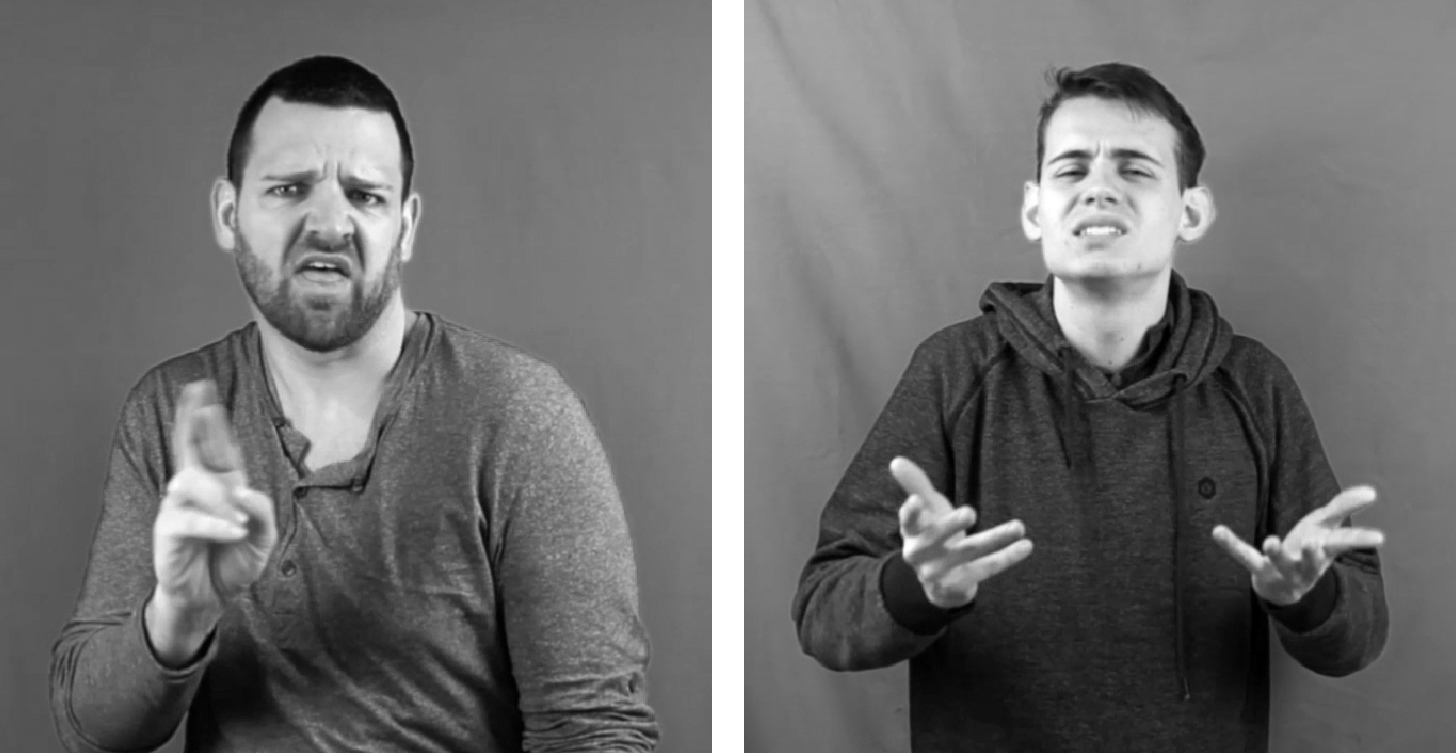
\includegraphics[width=1.0\textwidth]{nnmwhatwhosw.jpg}
	\caption{The non-manual markings used with constituent interrogatives in DGS consist of lowered brows and a squint. Additionally, the head is often put forwards towards the end of the clause. The signer on the left produces the sign \textsc{who}, the signer on the right the sign \textsc{what}.}
	\label{nnmwhatwho}
\end{figure}

As with polar interrogatives, the non-manuals used in \textit{wh}-questions have their intensity peak towards the end of the clause. This is true for the eyebrows and especially for moving the head forward, which mainly appears clause-finally. This is illustrated in Figure \ref{nnmwhatwhotwo}. The fact that the intensity peak is clause-final seems not to be influenced by the position of the \textit{wh}-phrase although in \textit{wh}-doubling, the clause-final \textit{wh}-phrase is typically focused. However, this seems not to be obligatory. Additionally, \textit{wh}-phrases may be focused in each position. 


\begin{figure}[bt]
\centering
	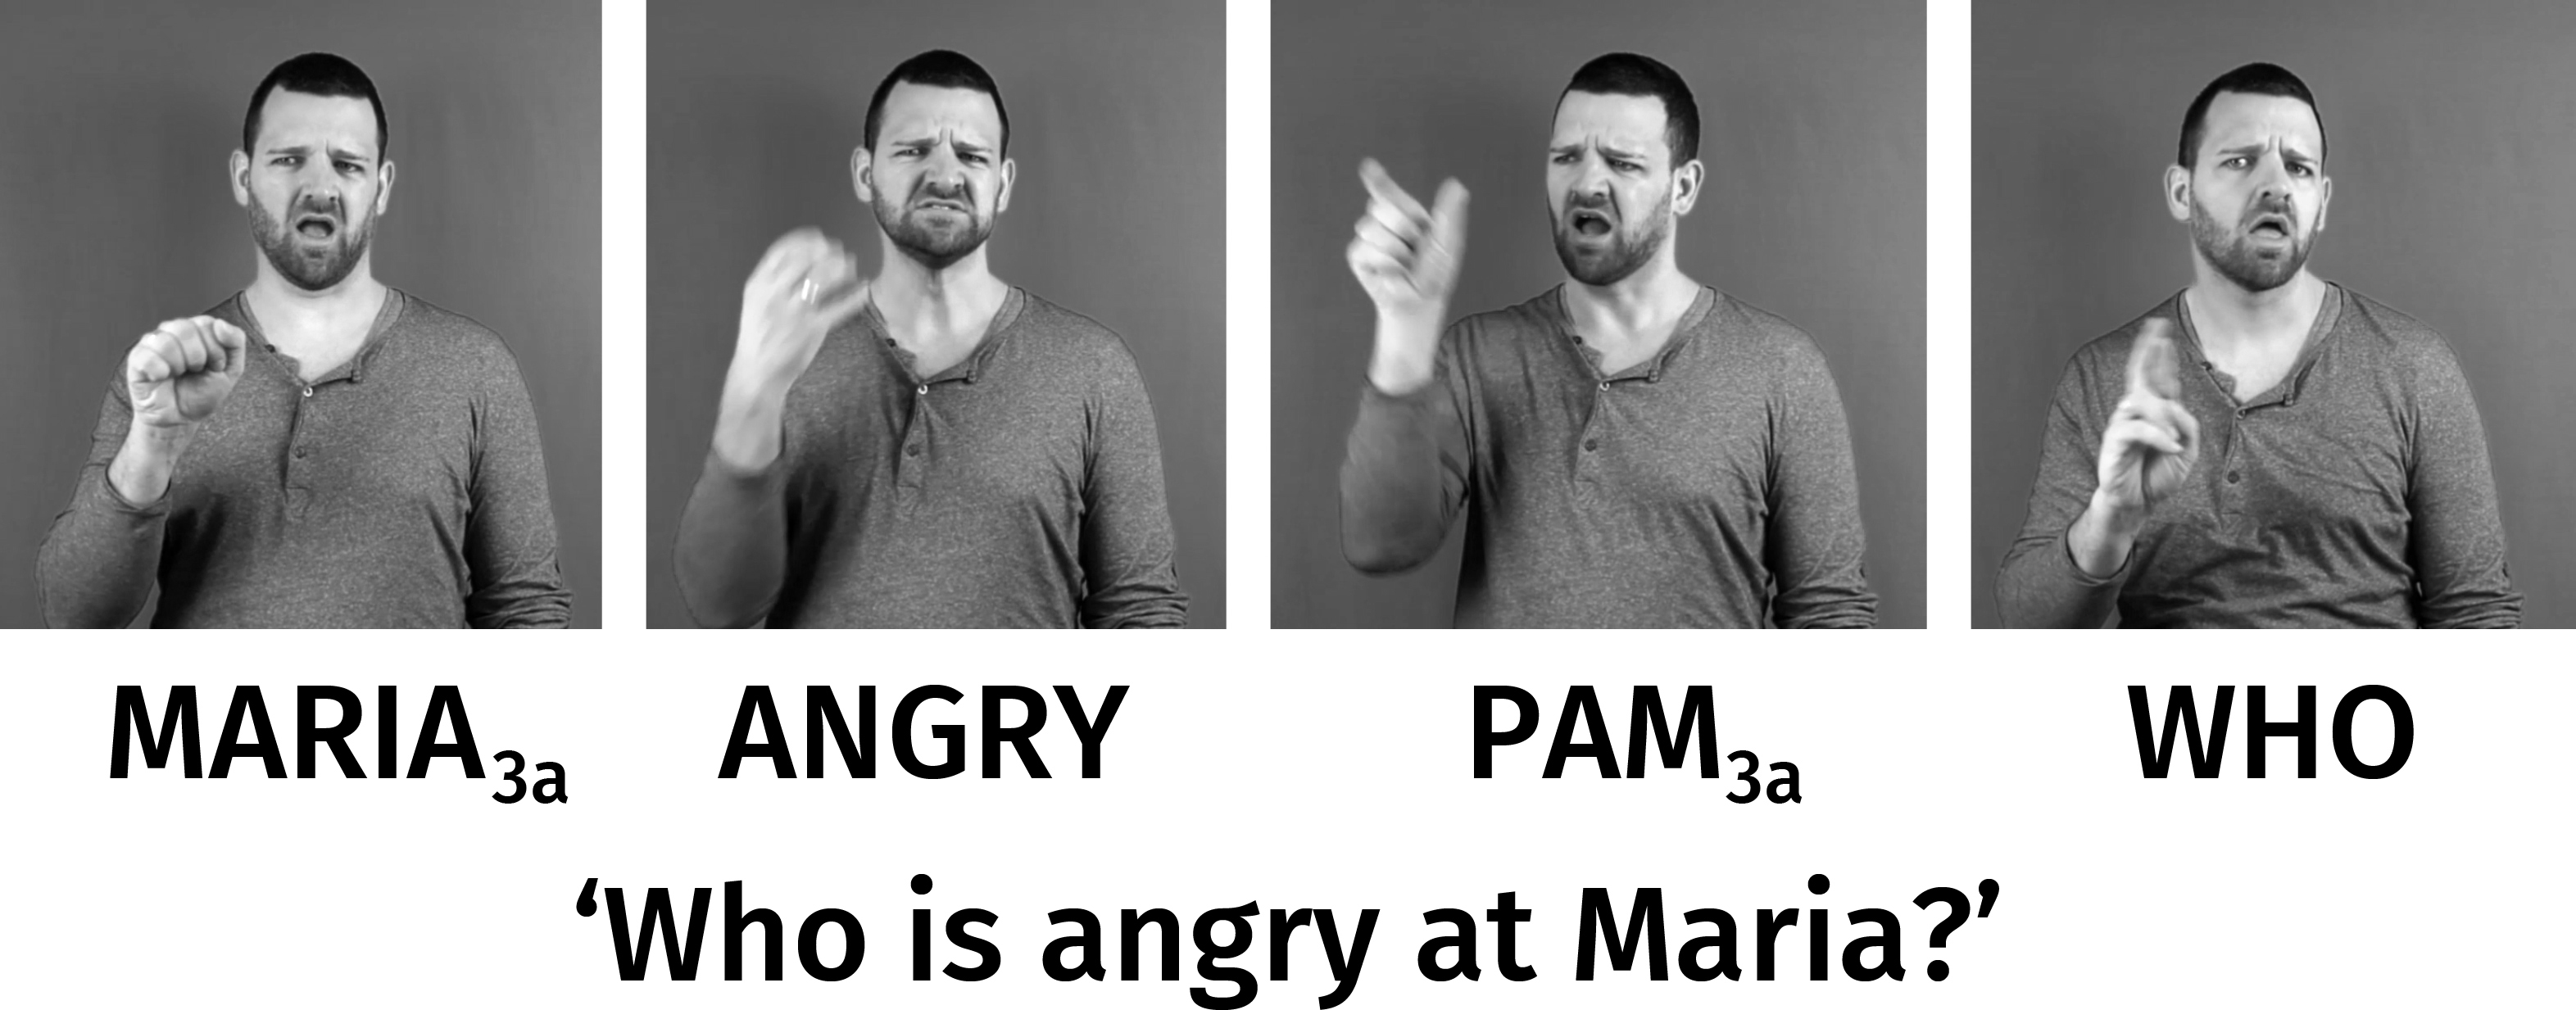
\includegraphics[width=1.0\textwidth]{whnonmanualsexamplesw.jpg}
	\caption{The non-manual markings used with constituent interrogatives have their intensity peak clause-finally. As with polar interrogatives the head is put forward (as can be seen in the last picture).}
	\label{nnmwhatwhotwo}
\end{figure}

A last note concerns slight head-shakes that often accompany \textit{wh}-signs in DGS. This pattern was noted for other sign languages as well. \citet[232--235]{sarac2007cross}, for example, observed head shakes on \textit{wh}-signs in \is{Croatian Sign Language}Croatian Sign Language. Similar to Croatian Sign Language, these head shakes in DGS only accompany the \textit{wh}-signs and do not spread further. Following \citet[235]{sarac2007cross}, I assume this head shake to be an ``assimilation with the movement of the hands'' as the hands often perform small repetitive movement with \textit{wh}-signs in DGS. Thus, I regard them to be a performance phenomenon and hence will not transcribe them.\footnote{Although I do not want to exclude the possibility completely that there might be some semantic import from these slight head shakes.}

\subsubsection{\textit{Wh}-signs in DGS}


%WH Signs
DGS has a whole paradigm of \textit{wh}-signs including \textsc{who}, \textsc{what}, \textsc{how}, \textsc{why}, \textsc{how-so} (German gloss \textsc{wieso}), \textsc{when}, \textsc{how-much}, \textsc{which}, \textsc{where}, \textsc{from-where}, and \textsc{to-where}. Note that some signers sign \textsc{which} with a Y-handshape and some simply use the sign for \textsc{what}. Nevertheless, complex \textit{wh}-phrases of the sort \textit{which computer} syntactically behave in the same way regardless of which manual sign is used. Phonologically, most of the \textit{wh}-signs consist of small repetitive movements of one or two hands or the fingers. An additional sign that often surfaces in \textit{wh}-questions is the so called `palm-up' gesture (glossed \textsc{p-ug}) that was already discussed for polar interrogatives (see Section \ref{polarinterrogativesdgs}) consisting of all fingers spread out with the palm facing upwards (using one or both hands). 

\subsubsection{Positions of \textit{wh}-elements in DGS}
%Position of the wh-elements

The literature on DGS mainly reports clause-final and clause-initial \textit{wh}-signs, as well as doubling (e.g., \citealt{papaspyrou2008grammatik, happ2014vork}). My own data shows that \textit{in-situ} questions are also possible. One use of \textit{wh-in-situ} are echo questions. This is true for real echo questions in which a signer has understood what s/he is echoing as well as information-seeking echo questions.\footnote{The difference between a real echo question and information-seeking echo questions is illustrated below -- note that it is unclear if the two types of echo questions actually behave differently in any language.

\begin{exe}
\ex\label{echoquestionillustrationenglish}\begin{xlist}
\ex A: Philip bought a new car.
\glt B: Philip bought a new \textsc{what}? He has no money to buy a new car! \label{echoquestionillustrationenglishb}
\ex A: Philip bought a new car.
\glt B: Philip bought a new \textsc{what}? I didn't understand you! \label{echoquestionillustrationenglisha}

\end{xlist}
\end{exe}

} However, I will leave echo questions aside in the following discussion.

A clause-structure theory of DGS %dealing with 
for constituent interrogatives should hence be able to explain -- at least -- the following possibilities. The unmarked position of \textit{wh}-phrases is the clause-final one, as in (\ref{ex:differentpositionsdgsa}). The example in (\ref{ex:differentpositionsdgsb}) shows that \textit{wh}-phrases can also occur clause-initially, although this is slightly marked as opposed to the clause-final pattern. The exact meaning differences between the clause-final and the clause-initial pattern have to be worked out. The third possibility that needs to be accounted for is doubling, shown in (\ref{ex:differentpositionsdgsaaaa}). 

\begin{exe}
\ex\label{differentpositionsdgs}
\begin{xlist} 
\ex \textcolor{white}{\%}\slg[wh]{yesterday beer buy who}
%
%\ex{} {\hspace{144pt}wh}  \\
%\textcolor{white}{\%}$\overline{\textrm{\textsc{yesterday beer buy who}}}$ 
\glt \textcolor{white}{\%}`Who bought beer yesterday?' \label{ex:differentpositionsdgsa} 
\ex \%\slg[wh]{who yesterday beer buy}
%
%\ex{} {\hspace{146pt}wh}  \\
%{\%$\overline{\textrm{\textsc{who yesterday beer buy}}}$} 
\glt \textcolor{white}{\%}`Who bought beer yesterday?' \label{ex:differentpositionsdgsb} 
\ex \textcolor{white}{\%}\slg[wh]{who yesterday beer buy who}
%
%\ex{} {\hspace{175pt}wh}  \\
%{} {\textcolor{white}{\%}$\overline{\textrm{\textsc{who yesterday beer buy who}}}$} 
\glt \textcolor{white}{\%}`Who bought beer yesterday?' \label{ex:differentpositionsdgsaaaa}
%\ex{} {\hspace{136pt}wh}  \\
%$\overline{\textrm{\textsc{yesterday who beer buy}}$}} 
%\glt `Who bought beer yesterday?' \label{ex:differentpositionsdgsc} 
\end{xlist}
\end{exe}

\noindent The fact that \textit{wh}-phrases can occur clause-finally, clause-initially, and can undergo doubling is in line with what was observed for other sign languages. Note that \textit{wh}-signs can receive focus regardless of position. However, when a \textit{wh}-sign is focused in a \textit{wh}-doubling construction it has to be the clause-final form that receives focus. In all cases, focus leads to a presuppositional reading. 

\begin{figure}[bt]
\centering
	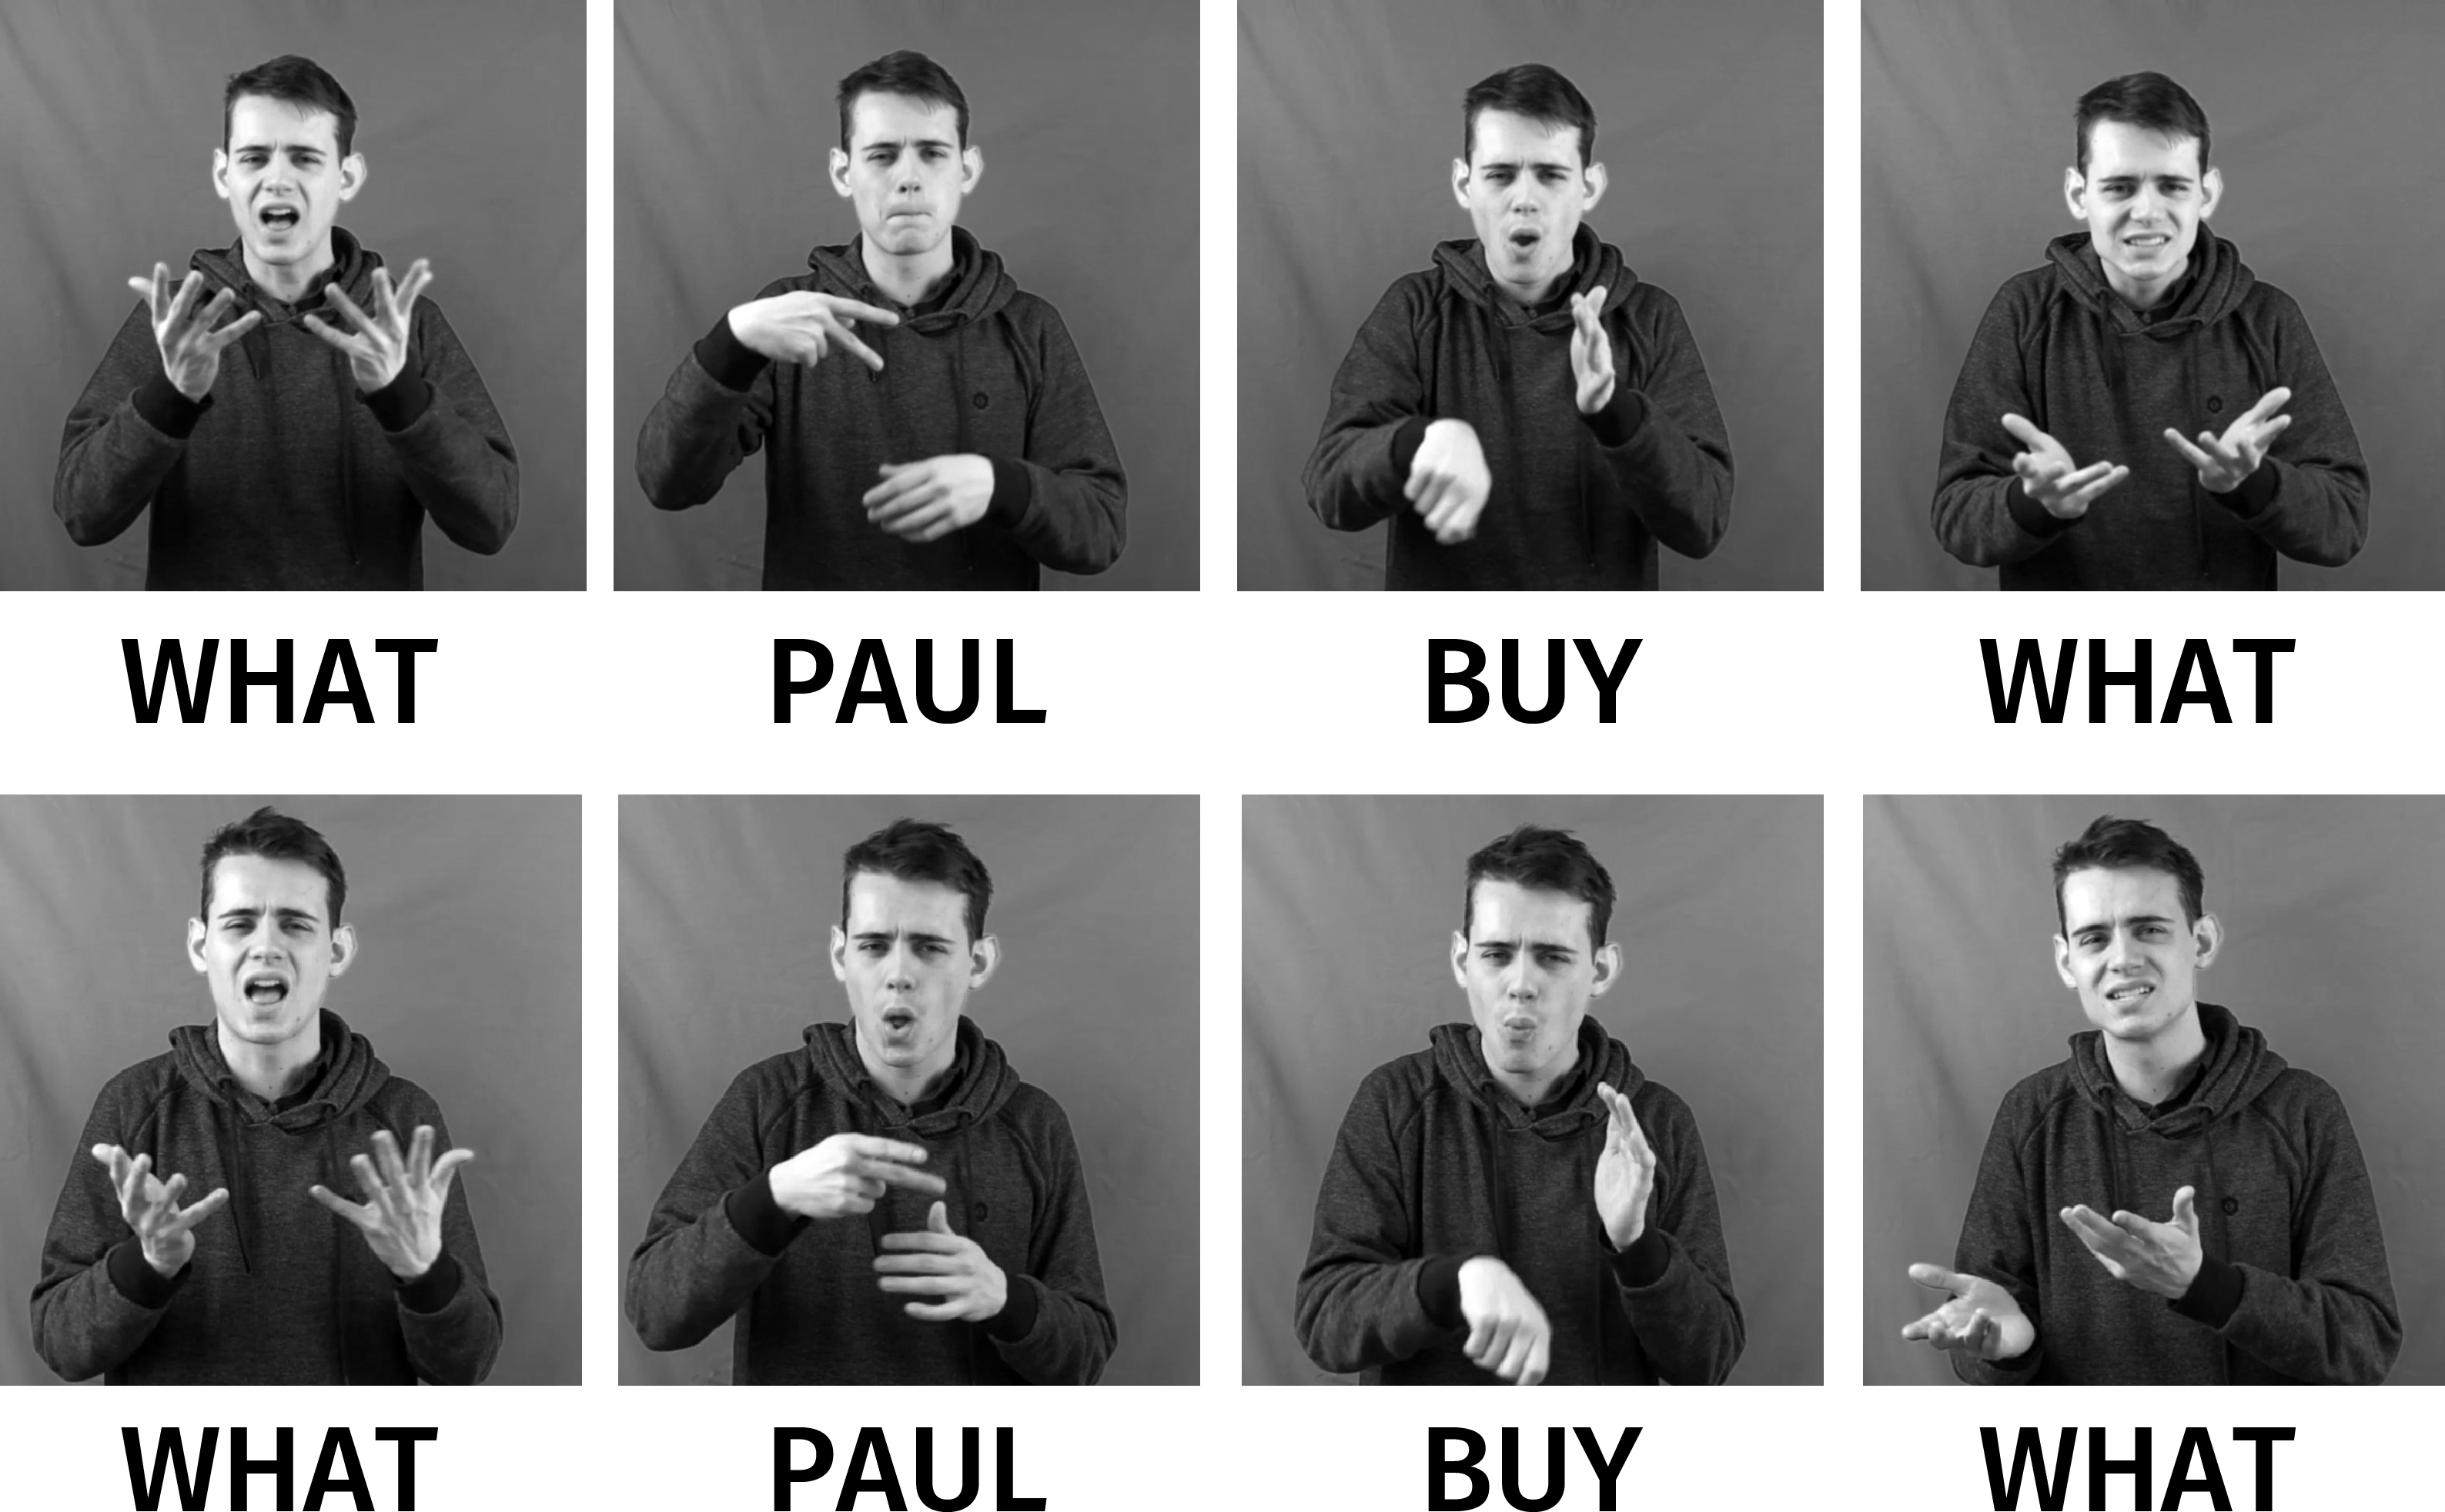
\includegraphics[width=1.0\textwidth]{whdoublingsw.jpg}
	\caption{With \textit{wh}-doubling two different patterns can be observed. In the first pattern, both \textit{wh}-signs are produced in neutral signing space. This is shown in the top example. In the second pattern, the first \textit{wh}-element is signed in neutral signing space (i.e., centered) while the second one is signed in a different position (on the side). This is shown in the bottom example. The examples show doubling in a sentence translating to \textit{What did Paul buy?}}
	\label{whdoubling}
\end{figure}

For \textit{wh}-doubling, two options are available. The first option consists of repeating the \textit{wh}-sign at the same location in signing space and for the second option, the clause-final sign is produced at a different location. Both types of \textit{wh}-doubling often receive an emphatic interpretation. Sentences in which the two instances are not produced in the same locations in signing space receive a (d-linked) set interpretation. Both cases are illustrated in Figure \ref{whdoubling}. The example at the bottom of the figure shows doubling with a set interpretation. This means that the signer indicates that it is clear to him that there is a set of items of which it is possible that Paul bought them and he wants to know which of this set Paul bought. The example at the top of the figure show doubling in the same location in signing space. 

\largerpage
Similar to what has been described for other sign languages, the picture that doubling presents in DGS is more complicated. As with \is{American Sign Language}American Sign Language, we find that doubling of complex \textit{wh}-phrases is not possible (\ref{ex:computerdoublinga}). Instead, it is possible to double only the simple \textit{wh}-phrase without its restrictor, as illustrated in (\ref{ex:computerdoublingb}). However, this pattern cannot be reversed, as in (\ref{ex:computerdoublingc}).


\begin{exe}
\ex\label{computerdoubling}
\begin{xlist} 
\ex *\slg[wh]{which computer paul buy which computer}
%
%\ex{} {\hspace{252pt}wh}  \\
%{} {*$\overline{\textrm{\textsc{which computer paul buy which computer}}}$} 
\glt \textcolor{white}{*}`Which computer did Paul buy?' \label{ex:computerdoublinga} 
\ex \textcolor{white}{*}\slg[wh]{which computer paul buy which}
%
%\ex{} {\hspace{188pt}wh}  \\
%{} {\textcolor{white}{*}$\overline{\textrm{\textsc{which computer paul buy which}}}$} 
\glt \textcolor{white}{*}`Which computer did Paul buy?' \label{ex:computerdoublingb} 
\ex *\slg[wh]{which paul buy which computer}
%
%\ex{} {\hspace{188pt}wh}  \\
%{} {*$\overline{\textrm{\textsc{which paul buy which computer}}}$} 
\glt \textcolor{white}{*}`Which computer did Paul buy?' \label{ex:computerdoublingc} 

\end{xlist}
\end{exe}

\noindent  Note that when no doubling is present, the \textit{wh}-phrase \textsc{which computer} is able to show up clause-initially or clause-finally. Interestingly, complex \textit{wh}-phrases show the exact opposite preferences as simple \textit{wh}-phrases. Thus, when no doubling is present, complex \textit{wh}-phrases systematically occur clause-initially, while the clause-final pattern, although well-formed, is the more marked version. This is shown in (\ref{computerdoublingonehundred}).

\begin{exe}
\ex\label{computerdoublingonehundred}
\begin{xlist} 
\ex \textcolor{white}{\%}\slg[wh]{which computer paul buy}
%
%\ex{} {\hspace{153pt}wh}  \\
%{} {\textcolor{white}{\%}$\overline{\textrm{\textsc{which computer paul buy}}}$} 
\glt \textcolor{white}{\%}`Which computer did Paul buy?' \label{ex:computerdoublingonehundreda} 
\ex \%\slg[wh]{paul buy which computer}
%
%\ex{} {\hspace{152pt}wh}  \\
%{} {\%$\overline{\textrm{\textsc{paul buy which computer}}}$} 
\glt \textcolor{white}{\%}`Which computer did Paul buy?' \label{ex:computerdoublingonehundredb} 
\end{xlist}
\end{exe}

\noindent Additionally, it is possible to move a \textit{wh}-element out of a complex \textit{wh}-phrase, as shown in (\ref{ex:splitexampledgs}). Thus, DGS shows what is traditionally called left-branch extraction \citep{bovskovic2005left, bovskovic2005locality}. Again, this extraction is only possible to the right, but not to the left (\ref{ex:splitexampledgsb}). However, the reason for sentence (\ref{ex:splitexampledgsb}) being ill-formed seems not to be due to syntactic reasons, but rather because of the fact that \textsc{which} and \textsc{paul} are adjacent which leads to the meaning \textit{which paul} which is not the desired meaning here.%\footnote{My consultants did not like this construction exactly because of this reason. Note however, that *\textsc{which paul} itself is ill-formed as asking for a specific person is achieved by \textsc{person who}.}


\begin{exe}
\ex\label{blablablahunderttausend}\begin{xlist}
\ex \textcolor{white}{??}\slg[wh]{paul \textup{\textit{t}}_{\textup{i}} computer buy which_{\textup{i}}}
%
%\ex {\hspace{166pt}wh}  \\
%{\textcolor{white}{??}$\overline{\textrm{\textsc{paul} \textit{t}\textsubscript{i} \textsc{computer buy which}\textsubscript{i}}}$} 
\glt \textcolor{white}{??}`Which computer did Paul buy?' \label{ex:splitexampledgs}
\ex ??\slg[wh]{which_{\textup{i}} paul \textup{\textit{t}}_{\textup{i}} computer buy}
%
%\ex {\hspace{166pt}wh}  \\
%{??$\overline{\textrm{\textsc{which}\textsubscript{i} \textsc{paul} \textit{t}\textsubscript{i} \textsc{computer buy}}}$} 
\glt \textcolor{white}{??}`Which computer did Paul buy?' \label{ex:splitexampledgsb}
\end{xlist}
\end{exe} 

\newpage 
\noindent Similar extraction facts were described for spoken languages as well (see the following side-note). Comparing the left-branch extraction in (\ref{ex:splitexampledgs}) with the partial doubling of complex \textit{wh}-phrases in (\ref{ex:computerdoublingb}) allows for different interpretations. Either one could call such structures partial doubling or interpret it as a complex clause-initial \textit{wh}-phrase plus left-branch extraction. Alternatively, the extracted \textsc{which} is an overt realization of operator movement that \citet{van2010complex} assumed to be empty in languages like English or German (see page \pageref{emptyoperator}). 

\begin{digression}{Left-branch extraction and determiners}{}
\noindent There is cross-linguistic variation as to the extraction of \textit{wh}-elements out of NP-/DP-internal constituents (see already \citealt{ross1967constraints}). This can be illustrated for complex \textit{wh}-phrases. While some languages do not allow movement of a \textit{wh}-element out of a complex constituent, others do allow this type of extraction, as illustrated in the English example in (\ref{leftbranchextractiona}) and the Serbo-Croatian example in (\ref{leftbranchextractionb}), both from \citet[14--15]{bovskovic2005left}. 



\begin{exe}
\ex\label{leftbranchextraction}\begin{xlist} 
\ex \textcolor{white}{*}English \\ *Whose\textsubscript{i} did you see $[$\textit{t}\textsubscript{i} father$]$? \label{leftbranchextractiona}
\ex \textcolor{white}{*}Serbo-Croatian \\ \gll {\textcolor{white}{*}\v{C}ijeg\textsubscript{i}} {si} {video} {$[$\textit{t}\textsubscript{i}} {oca$]$?}  \\
{\textcolor{white}{*}whose} {\textsc{clitic}} {seen} {} {father} \\
\trans \textcolor{white}{*}`Whose father did you see?' \label{leftbranchextractionb} 
\end{xlist}
\end{exe} 

\noindent The examples show that it is not possible for the \textit{wh}-word to move out of a \textit{wh}-phrase in English while this is allowed in Serbo-Croatian. \citet{bovskovic2005left, bovskovic2005locality} argues that the question of whether a language allows this so-called `left-branch extraction' or not is correlated with whether a language has overt determiners or not. In languages with overt determiners like English, so his argument, the DP forms a phase from which no extraction is allowed. In languages without overt determiners like Serbo-Croation, the DP does not form a phase and extraction is therefore allowed.

Like Serbo-Croation, DGS is a language lacking articles \citep[91]{happ2014vork} and similarly, DGS allows movement of a \textit{wh}-element out of a \textit{wh}-phrase as discussed above. Thus, DGS confirms \citeauthor{bovskovic2005left}'s (\citeyear{bovskovic2005left, bovskovic2005locality}) idea that languages without overt articles allow left-branch extraction.

Similar splits between a \textit{wh}-sign and its restriction were observed in other (articleless) sign languages as well. In \is{Italian Sign Language}Italian and \is{Japanese Sign Language}Japanese Sign Language, for example, this is equally possible, as the example in (\ref{ex:splitexamplelisa}) from \citet[285]{cecchetto2009another} and the example in (\ref{ex:splitexamplelisb}) from \citet{fischer1998feature} cited in \citet[25]{zeshan2004interrogative} illustrate (\citealt{zeshan2004interrogative} also mentions that \is{American Sign Language}American Sign Language and \is{Indo-Pakistani Sign Language}Indo-Pakistani Sign Language allow for similar structures; for American Sign Language see also \citealt{boster1996quantifier}). 

\begin{exe}
\ex\label{splitexamplelis}\begin{xlist}
\ex Italian Sign Language \\\slg{boy book steal} \slg[wh]{which}
%\ex {} {\hspace{119pt}wh}  \\
%{\textsc{boy book steal}} {$\overline{\textrm{\textsc{which}}}$} 
\glt `Which boy stole the book?' \label{ex:splitexamplelisa} 
\ex Japanese Sign Language \\ \slg{color like} \slg[wh]{what}
%\ex {} {\hspace{85pt}wh}  \\
%{\textsc{color} \textsc{like} {$\overline{\textrm{\textsc{what}}}$}} 
\glt `Which color do you like?' \label{ex:splitexamplelisb} 
\end{xlist}
\end{exe} 

\noindent These examples show that in the case of left-branch extraction, articleless sign languages behave just as articleless spoken languages. 
\end{digression}


\noindent As with simple \textit{wh}-phrases (e.g., \textsc{what}) and in contrast to complex \textit{wh}-phrases (e.g., \textsc{which computer}), \textit{wh}-phrases contained in a PP may occur in a clause-final and -initial position as illustrated in (\ref{whphrasesinappdgs}), again with the clause-initial version being the slightly more marked one. Note that I analyze the signs \textsc{pam} and \textsc{bem} as being prepositions or preposition-like elements here (with \textsc{pam} meaning `at' and \textsc{bem} meaning `for'). See also the brief descriptions of the signs in the Section of notational conventions (on page \pageref{notational}).


%(note that the sign \textsc{pam}, an abbreviation for `person agreement marker' \citep{rathmann2003optionality}, is traditionally described as marking verb agreement)

%\hspace{-0.75cm}\begin{minipage}[t]{0.9\textwidth}
\begin{exe}
\ex\label{whphrasesinappdgs}
%\setlength{\columnsep}{1.5cm}
%\begin{multicols}{2}
\begin{xlist}
%$\overline{\textrm{}}$
\ex \textcolor{white}{\%}\slg[wh]{index_2 angry pam who}
%
%\ex {\hspace{129pt}wh}  \\
%{{\textcolor{white}{\%}$\overline{\textrm{\textsc{index}\textsubscript{2} \textsc{angry pam who}}}$}} 
\glt {\textcolor{white}{\%}`At whom are you angry?' \label{whphrasesinappdgsb}}
\ex \%\slg[wh]{pam who index_2 angry}
%
%\ex {\hspace{129pt}wh}  \\
%{\%$\overline{\textrm{\textsc{pam who index}\textsubscript{2} \textsc{angry}}}$} 
\glt {\textcolor{white}{\%}`At whom are you angry?' \label{whphrasesinappdgsa}}
\end{xlist}
%\end{multicols}
\end{exe}
%\end{minipage}


\noindent Crucially, phrases such as \textsc{which computer} are not syntactic operators as introduced in Section \ref{syntaxoperators} while simple \textit{wh}-phrases and \textit{wh}-phrases included in a PP are. This would predict that doubling of \textit{wh}-PPs should be acceptable in DGS. And indeed, doubling of a \textit{wh}-PP is possible, as illustrated in (\ref{doublingphrases}) and additionally in Figure \ref{whdoublinggg}. 

\begin{figure}[bt]
\centering
	\includegraphics[width=0.9\textwidth]{doublingsw.jpg}
	\caption{Examples of doubling of \textit{wh}-phrases contained in a PP.}
	\label{whdoublinggg}
\end{figure}

Note that I indicated that the examples are marked. In fact, signers judged the examples from being absolutely well-formed to being rather marked, but not ill-formed. This is in line with the observations on the doubling of PP-\textit{wh}-phrases in German (see page \pageref{whcopyinggermanb}) and in Northern Italian dialects (see page \pageref{morenorthernitalianab}). Also note that some, but not all signers reported that the acceptability improves with a short intonational break before the double, as indicated by the bracketed commas (similar to the Northern Italian examples).\footnote{See \citet[324--325]{happ2014vork} for similar doubling examples discussed in different contexts. } 


\begin{exe}
\ex\label{doublingphrases}
\begin{xlist} 
\ex \%\slg[wh]{pam who index_2 angry(,) pam who}
%
%\ex{} {\hspace{199pt}wh}  \\
%{} {\%$\overline{\textrm{\textsc{pam who index}\textsubscript{2} \textsc{angry(,) pam who}}}$} 
\glt \textcolor{white}{\%}`At whom are you angry?' \label{ex:doublingphrasesa} 
\ex \%\slg[wh]{bem who index_2 cook(,) bem who}
%
%\ex{} {\hspace{195pt}wh}  \\
%{} {\%$\overline{\textrm{\textsc{bem who index}\textsubscript{2} \textsc{cook(,) bem who}}}$} 
\glt \textcolor{white}{\%}`For whom do you cook?' \label{ex:doublingphrasesb} 
\ex \%\slg[wh]{with who index_2 cook(,) with who}
%
%\ex{} {\hspace{206pt}wh}  \\
%{} {\%$\overline{\textrm{\textsc{with who index}\textsubscript{2} \textsc{cook(,) with who}}}$} 
\glt \textcolor{white}{\%}`With who do you cook?' \label{ex:doublingphrasesc} 
\end{xlist}
\end{exe}

\noindent Thus, with respect to the doubling of \textit{wh}-phrases contained in a PP, DGS patterns with Northern Italian dialects and with spoken German. 



\largerpage
\subsubsection{Analyzing the DGS data}

\noindent It is admittedly not easy to account for all the aforementioned facts in a syntactic model. For ease of understanding, I summarize the relevant facts that need to be accounted for in (\ref{overvieswhtypes}).

\begin{exe}
\ex\label{overvieswhtypes}
\begin{xlist}
\ex \textcolor{white}{\%}\textit{Clause-final simple \textit{wh}-phrase:}\\
\textcolor{white}{\%}\slg[wh]{today \textup{\textit{t}}_{\textup{i}} beer buy who_{\textup{i}}}
\label{overvieswhtypesa}
\ex \textcolor{white}{\%}\textit{Clause-initial simple \textit{wh}-phrase (slightly marked):}\\
\%\slg[wh]{who_{\textup{i}} (today) \textup{\textit{t}}_{\textup{i}} beer buy}
\label{overvieswhtypesb}
\ex \textcolor{white}{\%}\textit{Doubling of a simple \textit{wh}-phrase:}\\
\textcolor{white}{\%}\slg[wh]{who_{\textup{i}} (today) \textup{\textit{t}}_{\textup{i}} beer buy who}
\label{overvieswhtypesc}
\ex \textcolor{white}{\%}\textit{Clause-initial complex \textit{wh}-phrase:}\\
\textcolor{white}{\%}\slg[wh]{[which car]_{\textup{i}} paul \textup{\textit{t}}_{\textup{i}} buy}
\label{overvieswhtypesd}
\ex \textcolor{white}{\%}\textit{Left-branch extraction to the right:}\\
\textcolor{white}{\%}\slg[wh]{paul \textup{\textit{t}}_{\textup{i}} car buy which_{\textup{i}}}
\label{overvieswhtypese}
\ex \textcolor{white}{\%}\textit{Illicit left-branch extraction to the left:}\\
??\slg[wh]{which_{\textup{i}} paul \textup{\textit{t}}_{\textup{i}} car buy}
\label{overvieswhtypesf}
\ex \textcolor{white}{\%}\textit{Clause-final complex \textit{wh}-phrase (slightly marked):}\\
\textcolor{white}{*}\%\slg[wh]{paul \textup{\textit{t}}_{\textup{i}} buy [which car]_{\textup{i}}}
\label{overvieswhtypesg}
\ex \textcolor{white}{*\%}\textit{Illicit complex doubling:} \\
\textcolor{white}{\%}*\slg[wh]{[which car]_{\textup{i}} paul \textup{\textit{t}}_{\textup{i}} buy [which car]_{\textup{i}}}
\label{overvieswhtypesh}
\ex \textcolor{white}{*\%}\textit{Initial complex \textit{wh} $+$ extraction:} \\
\textcolor{white}{*\%}\slg[wh]{[which car]_{\textup{i}} paul \textup{\textit{t}}_{\textup{i}} buy which_{\textup{i}}}
\label{overvieswhtypesi}
\ex \textcolor{white}{*\%}\textit{Final complex \textit{wh} $+$ extraction:} \\
\textcolor{white}{\%}*\slg[wh]{which_{\textup{i}} paul \textup{\textit{t}}_{\textup{i}} buy [which car]_{\textup{i}}}
\label{overvieswhtypesj}

\end{xlist}

\end{exe}

\noindent The examples from (\ref{overvieswhtypesa}) to (\ref{overvieswhtypesc}) are, as discussed, the ones that could also contain a \textit{wh}-phrase contained in a PP (e.g., \textsc{with who}). Thus, it is clear that we need to provide two specifier positions. The bracketed temporal adverbs indicate the clause-initial position in declarative sentences. The structure in (\ref{overvieswhtypesd}) is the neutral way to ask a question containing a complex \textit{wh}-phrase, (\ref{overvieswhtypese}) shows a left-branch extraction, (\ref{overvieswhtypesf}) the illicit left-branch extraction. The example in (\ref{overvieswhtypesg}) shows a slightly marked, but grammatical construction with a clause-final complex \textit{wh}-phrase. In (\ref{overvieswhtypesh}), the illicit doubling of a complex \textit{wh}-phrase is illustrated and (\ref{overvieswhtypesi}) shows the possible doubling. Finally, (\ref{overvieswhtypesj}) shows that the opposite option with an extracted simple \textit{wh}-element clause-initially and a clause-final complex \textit{wh}-phrase is not a licit structure in DGS.

% \todo{multiply defined refs}
In the following I will propose two different models to account for the data in (\ref{overvieswhtypes}). The first model will follow the rightward-movement tradition and the second model will follow the Kayneian idea that the order specifier--head--com\-ple\-ment is fixed (thus, all heads will be left-headed and all specifiers will also be to the left). Both accounts will need to make use of remnant movement.

\subsubsection{Syntactic analyses: two possiblities}

If we follow the van Craenenbroek model, we would assume that CP\textsubscript{1}, but not CP\textsubscript{2} is a possible host for complex \textit{wh}-phrases. Similar to Strijen Dutch (see page \pageref{vancraenenbroekdutchdialecta}), the general landing site for simple \textit{wh}-phrases and \textit{wh}-phrases contained in a PP is CP\textsubscript{2}. These assumptions will hold for both models.

I will first show how to implement this in a mixed-branching structure. SpecCP\textsubscript{2} is right-branching in this model, as \textit{wh}-phrases obviously occur to the right in DGS. In contrast to simple \textit{wh}-phrases and \textit{wh}-phrases contained in a PP, complex \textit{wh}-phrases cannot be hosted in CP\textsubscript{2} (again similar to Strijen Dutch), but are base-generated in CP\textsubscript{1}, that I take to be the mirror image of CP\textsubscript{2}, i.e., left-branching (note that I simply posit that the heads are on the same side as the specifiers in the following). 

A simple constituent interrogative like \textsc{beer buy who} is then derived by moving the \textit{wh}-phrase \textsc{who} to SpecCP\textsubscript{2}, as shown in (\ref{ex:firstanalysisababaa}). A clause-initial constituent interrogative like \textsc{who beer buy} is derived by first moving the \textit{wh}-phrase \textsc{who} to SpecCP\textsubscript{2} and from there, in a cyclic fashion, to SpecCP\textsubscript{1}. In this case, the intermediate copy of \textsc{who} (in SpecCP\textsubscript{2}) is deleted. Additionally, it is possible to spell out this copy resulting in a doubling construction (\textsc{who beer buy who}). These options are shown in (\ref{ex:firstanalysisababab}). The optional deletion of the copy in SpecCP\textsubscript{2} is indicated by the gray color of the \textit{wh}-phrase.

%%%%%%%%%%%%%%%%%%%%%%%%%%%%
%\clearpage
%%%%%%%%%%%%%%%%%%%%%%%%%%%%

One advantage of this modeling possibility is that the more marked case, i.e. sentences containing a clause-initial simple \textit{wh}-phrase, needs an additional movement step (as well as the doubling construction which is generally more marked than a \textit{wh}-question with only one \textit{wh}-phrase).




\begin{exe}
\ex\label{ex:firstanalysisababa}
\begin{xlist}

\ex \label{ex:firstanalysisababaa}
\parbox[t]{.3\textwidth}{
\hspace*{-2cm}
\begin{forest}
for tree={s sep=2mm, inner sep=0, l=5mm} %s sep = Breite; l = Höhe
[{CP\textsubscript{1}} [SpecCP\textsubscript{1} [{who\textsubscript{i}}, roof, name=cp1] ] [{$\overline{\textrm{C\textsubscript{1}}}$} [{C\textsubscript{1}\textdegree} ] [{CP\textsubscript{2}} [{$\overline{\textrm{C\textsubscript{2}}}$} [IP [{$\textrm{\textit{t}}$\textsubscript{i} \textsc{beer buy}}, roof, name=start]] [{C\textsubscript{2}\textdegree} ] ] [SpecCP\textsubscript{2} [{\textsc{who}\textsubscript{i}}, roof, name=end] ] ] ] ]
%\draw[->] (start) to[out=west,in=south] (end);
\draw[semithick,->] (start)..controls +(west:3) and +(south:4)..(end);
\node (text) at (0.10,-6.6) {\slg[wh]{beer buy who}};%\end{forest}
\end{forest}
}
\parbox[t]{.5\textwidth}{
\vspace{-.7\baselineskip}
\ex\label{ex:firstanalysisababab}
\hspace*{-1cm}
\begin{forest}
for tree={s sep=5mm, inner sep=0, l=5mm} %s sep = Breite; l = Höhe
[{CP\textsubscript{1}} [SpecCP\textsubscript{1} [{\textsc{who}\textsubscript{i}}, roof, name=cp1] ] [{$\overline{\textrm{C\textsubscript{1}}}$} [{C\textsubscript{1}\textdegree} ] [{CP\textsubscript{2}} [{$\overline{\textrm{C\textsubscript{2}}}$} [IP [{$\textrm{\textit{t}}$\textsubscript{i} \textsc{beer buy}}, roof, name=ip] ] [{C\textsubscript{2}\textdegree} ] ] [SpecCP\textsubscript{2} [{\textcolor{gray}{\textsc{who}\textsubscript{i}}}, roof, name=cp2]  ] ] ] ]
\draw[semithick,->] (ip)..controls +(west:3) and +(south:4)..(cp2);
\draw[semithick,->] (cp2)..controls +(south west:9) and +(west:3)..(cp1);
\node (text) at (0.5,-6.5) {\slg[wh]{who beer buy (who)}};
\end{forest}
}
\end{xlist}
\vspace*{-2.5cm}
\end{exe} 





\noindent The next step is to account for complex \textit{wh}-phrases like \textsc{which computer}. Under the assumption that complex \textit{wh}-phrases are base-generated in SpecCP\textsubscript{1}, we simply get the structure in (\ref{ex:xfirstanalysisaba}). Following van Craenenbroek's ideas completely, one could assume empty operator movement in this case too. Additionally, it is possible to account for left-branch extraction, as shown in (\ref{ex:firstanalysisabb}). This case could be seen as an overt manifestation of the empty operator movement. Combining the two mechanisms results in the partial doubling found with complex \textit{wh}-phrases (e.g., \textsc{which computer paul buy which}). %Thus, the empty operator movement van Craenenbroek (2010) assumed, is visible in DGS.

The structures in (\ref{ex:firstanalysisabx}) also account for the ill-formedness of doubling in cases of complex \textit{wh}-phrases, as there is only one possible host for this type of \textit{wh}-phrase, namely SpecCP\textsubscript{1}. Left-branch extraction to the left, however, should be possible in principle. And indeed, it is (this would probably be cyclical as well). However, extracting the operator to the left makes it adjacent to the first sign in the sentence that, in this case, leads to the odd reading `Which Paul is buying a computer?' 

\clearpage 
\begin{exe}
\ex\label{ex:firstanalysisabx}
\begin{multicols}{2}
\begin{xlist}
\ex \label{ex:xfirstanalysisaba}
\hspace*{-1.5cm}
\begin{forest}
for tree={s sep=5mm, inner sep=0, l=5mm} %s sep = Breite; l = Höhe
[{CP\textsubscript{1}} [SpecCP\textsubscript{1} [{\textsc{which computer}\textsubscript{i}}, roof, name=cp1] ] [{$\overline{\textrm{C\textsubscript{1}}}$} [{C\textsubscript{1}\textdegree} ] [{CP\textsubscript{2}} [{$\overline{\textrm{C\textsubscript{2}}}$} [IP [{\textsc{paul} \textsc{buy}}, roof, name=ip] ] [{C\textsubscript{2}\textdegree} ] ] [SpecCP\textsubscript{2} [{\textcolor{white}{who\textsubscript{i}}}, roof, name=cp2] ] ] ] ]
\node (text) at (0.10,-5.4) {\slg[wh]{which computer paul buy}};
\end{forest}
\ex\label{ex:firstanalysisabb}
\hspace*{-5mm}
\begin{forest}
for tree={s sep=5mm, inner sep=0, l=5mm} %s sep = Breite; l = Höhe
[{CP\textsubscript{1}} [SpecCP\textsubscript{1} [{\textcolor{white}{\textsc{computer}\textsubscript{i}}}, roof, name=cp1] ] [{$\overline{\textrm{C\textsubscript{1}}}$} [{C\textsubscript{1}\textdegree} ] [{CP\textsubscript{2}} [{$\overline{\textrm{C\textsubscript{2}}}$} [IP [{\textsc{paul} $\textrm{\textit{t}}$\textsubscript{i} \textsc{computer buy}}, roof, name=ip] ] [{C\textsubscript{2}\textdegree} ] ] [SpecCP\textsubscript{2} [{\textsc{which}\textsubscript{i}}, roof, name=cp2] ] ] ] ]
\draw[semithick,->] (ip)..controls +(south west:0.1) and +(south:2.8)..(cp2);
\node (text) at (0.8,-5.4) {\slg[wh]{paul \textup{\textit{t}}_{\textup{i}} computer buy which_{\textup{i}}}};
\end{forest}
\end{xlist}
\end{multicols}
\vspace*{-.5cm}
\end{exe}




The last thing to model is a clause-final complex \textit{wh}-phrase. For this, an additional remnant movement needs to be assumed. The tree in (\ref{remnantmovementoftheipwithtwocps}) shows how this could be implemented in the current model. It is, however, unclear into which position this movement would be, but one could assume that it is SpecForceP. 

\begin{exe}
\ex\label{remnantmovementoftheipwithtwocps}
\resizebox{.92\textwidth}{!}{
\begin{forest}
for tree={s sep=15mm, inner sep=0, l=10mm} %s sep = Breite; l = Höhe
[ForceP [SpecForceP [{\textcolor{white}{something here}}, roof, name=sleepyman]] [{$\overline{\textrm{Force}}$} [{Force\textdegree} ] [{CP\textsubscript{1}} [SpecCP\textsubscript{1} [{\textsc{which computer}\textsubscript{i}}, roof, name=cp1] ] [{$\overline{\textrm{C\textsubscript{1}}}$},tikz={\node [draw,gray,fit to=tree]{};} [{C\textsubscript{1}\textdegree} ] [{CP\textsubscript{2}} [{$\overline{\textrm{C\textsubscript{2}}}$} [IP [{\textsc{paul} \textcolor{white}{$\textrm{\textit{t}}$\textsubscript{i}} \textsc{buy}}, roof, name=ip] ] [{C\textsubscript{2}\textdegree} ] ] [SpecCP\textsubscript{2} [{\textcolor{white}{\textsc{which}\textsubscript{i}}}, roof, name=cp2] ] ] ] ] ] ] 
%\draw[semithick,->] (ip)..controls +(south:2) and +(south:4)..(cp1);
%\draw[semithick, <-] (cp2.south) to [bend right=-60] (ip.base west);
\node (A) at (5.6,-7.15) {};
%\draw[semithick,->] (A)..controls +(south:3) and +(south:4)..(sleepyman);
%\draw[semithick,->] (ip.south) to [bend right=-80] node [midway,fill=white] {Step 1} (cp1.south);
%\draw[semithick,->] (A)..controls +(south west:0.1) and +(south:4)..(sleepyman);
\draw[semithick,->] (A.south) to [bend right=-80] (sleepyman.south);
%\draw[gray] (7.6,-7.1) circle (4cm);
\end{forest}
}
\vspace*{-1cm}
\end{exe}

%\begin{exe}
%\ex\label{remnantmovementoftheipwithtwocps}
%\begin{adjustbox}{max width=0.80\textwidth}
%\begin{tikzpicture}[baseline]
%\tikzset{level distance=40pt,sibling distance=10pt}
%\Tree [.ForceP [.SpecForceP \edge[roof]; \node(sleepyman){\textcolor{white}{something here}}; ] [.{$\overline{\textrm{Force}}$} [.{Force\textdegree} ] [.{CP\textsubscript{1}} [.SpecCP\textsubscript{1} \edge[roof]; \node(cp1){\textsc{which computer}\textsubscript{i}}; ] [.{$\overline{\textrm{C\textsubscript{1}}}$} [.{C\textsubscript{1}\textdegree} ] [.{CP\textsubscript{2}} [.{$\overline{\textrm{C\textsubscript{2}}}$} [.IP \edge[roof]; \node(ip){\textsc{paul} \textcolor{white}{$\textrm{\textit{t}}$\textsubscript{i}} \textsc{buy}}; ] [.{C\textsubscript{2}\textdegree} ] ] [.SpecCP\textsubscript{2} \edge[roof]; \node(cp2){\textcolor{white}{\textsc{which}\textsubscript{i}}}; ] ] ] ] ] ] 
%
%%\draw[semithick,->] (ip)..controls +(south:2) and +(south:4)..(cp1);
%%\draw[semithick, <-] (cp2.south) to [bend right=-60] (ip.base west);
%
%\node (A) at (7.6,-11.0) {};
%%\draw[semithick,->] (A)..controls +(south:3) and +(south:4)..(sleepyman);
%%\draw[semithick,->] (ip.south) to [bend right=-80] node [midway,fill=white] {Step 1} (cp1.south);
%%\draw[semithick,->] (A)..controls +(south west:0.1) and +(south:4)..(sleepyman);
%\draw[semithick,->] (A.south) to [bend right=-80] (sleepyman.south);
%\draw[gray] (7.6,-7.1) circle (4cm);
%
%\end{tikzpicture}
%\end{adjustbox}
%\end{exe}
%
%\vspace{-0.8cm}

\newpage 
\noindent The additional remnant movement is not that farfetched as the resulting structure is more marked than the clause-initial one. Thus, again, a marked structure is derived by an additional movement step.

One open point is the spreading behavior of the non-manuals. Considering the insights gained about polar interrogatives from the previous section, we could say that the IntP is located above the \textit{wh}-landing sites. The spreading of the non-manuals can, again, be assumed to be regulated by Int\textdegree\ which should be right-headed to account for the non-manuals being strongest clause-finally. This is indeed the case. Additionally, \textit{wh}-question in DGS can always be followed by \textsc{p-ug}. This sign was also described for constituent interrogatives in other sign languages. Notably, \citet{aboh2010sa} analyze the clause-final palm-up gesture in \textit{wh}-questions in the \is{Sign Language of the Netherlands}Sign Language of the Netherlands as an instantiation of Inter\textdegree . In Sign Language of the Netherlands and in DGS, the palm-up gesture is found in the very last position of the clause. Compare the data from \citet[111]{aboh2010sa} in (\ref{ex:abohpfaupug}) and the DGS examples in (\ref{pugdgs}).

\begin{exe}
\ex Sign Language of the Netherlands \citep[111]{aboh2010sa} \\ \slg[wh]{poss_2 bike steal who p-ug}
\glt `Who stole your bike?' \label{ex:abohpfaupug} 

\ex\label{pugdgs}
\begin{xlist} 
\ex \slg[wh]{maria angry pam who p-ug}
%\ex {\hspace{148pt}wh}  \\
%$\overline{\textrm{\textsc{maria angry pam who p-ug}}}$ 
\glt `At whom is Maria angry?' \label{ex:pugdgsa} 
\ex \slg[wh]{who pam maria angry p-ug}
%\ex {\hspace{148pt}wh}  \\
%$\overline{\textrm{\textsc{who pam maria angry p-ug}}}$
\glt `Who is angry at Maria?' \label{ex:pugdgsb} 
\end{xlist}
\end{exe}

\noindent Thus, if \textsc{p-ug} is indeed located in Inter\textdegree\ and if this head is also triggering the non-manuals in constituent interrogatives, the proposed model is completely in line with the data. Assuming that the non-manuals are triggered by Inter\textdegree\ in both, polar and constituent questions, however, poses the question why the non-manuals in polar and constituent questions differs in DGS. I will leave this open for further research.   %Especially, when taking into account that focused \textit{wh}-signs in doubling constructions are also accompanied by 

Alternatively, a similar idea would be to model \textit{wh}-movement in DGS similar to what was proposed for Northern Italian earlier (cf. page \pageref{italianwhdoublinga}), i.e., with an additional projection between CP\textsubscript{1} and CP\textsubscript{2}. While this model clearly is more elegant, as it is possible to construct it in a more Kayneian way (with all specifiers and heads to the left) it has the disadvantage of requiring a lot more (remnant) movement steps that are hard to motivate and an additional projection. The overall model would have the structure in (\ref{remnantmovementitalianstyle}).%If one tries to motivate this remnant movement along similar lines as Aboh \& Pfau (2010), namely by assuming that there is a strong Int\textdegree\ that attracts the remnant into it's specifier, the structure would in general look like the following. 

In this model, it has to be assumed that after all movement steps are completed, the remainder of the clause is moved into the specifier of the InterP. Assuming that it is feature checking between SpecInterP and Inter\textdegree\ that triggers the non-manual markings, all material is accompanied by brow lowering with the intensity peak being clause-final. 

%\vspace{-0.3cm}



\begin{exe}
\ex\label{remnantmovementitalianstyle}
\begin{forest}
for tree={s sep=7mm, inner sep=0, l=5mm} %s sep = Breite; l = Höhe
[{InterP} [SpecInterP [{\phantom{NNN}}, roof, name=specintp] ] [{$\overline{\textrm{Int}}$} [{Inter\textdegree } ] [{CP\textsubscript{1}} [SpecCP\textsubscript{1} [{\phantom{NNN}}, roof, name=speccp1] ] [{$\overline{\textrm{CP\textsubscript{1}}}$} [{C\textsubscript{1}\textdegree} ] [{XP} [SpecXP [{\phantom{NNN}}, roof, name=specintp2] ] [{$\overline{\textrm{X}}$} [{X\textdegree } ] [{CP\textsubscript{2}} [SpecCP\textsubscript{2} [{\phantom{NNN}}, roof, name=speccp2]] [{$\overline{\textrm{CP\textsubscript{2}}}$} [{C\textsubscript{1}\textdegree} ] [IP [{\phantom{NNN}}, roof, name=ip] ] ] ] ] ] ] ] ] ]
%[.IP \edge[roof]; \node(ip){\textsc{paul} $t$\textsubscript{i} \textsc{buy}}; 
\end{forest}
\end{exe}
%
%\begin{exe}
%\ex\label{remnantmovementitalianstyle}
%\begin{adjustbox}{max width=0.90\textwidth}
%\begin{tikzpicture}[baseline]
%\tikzset{level distance=35pt,sibling distance=10pt}
%\Tree [.{InterP} [.SpecInterP \edge[roof]; \node(specintp){\textcolor{white}{something here}}; ] [.{$\overline{\textrm{Int}}$} [.{Inter\textdegree } ] [.{CP\textsubscript{1}} [.SpecCP\textsubscript{1} \edge[roof]; \node(speccp1){\textcolor{white}{something here}}; ] [.{$\overline{\textrm{CP\textsubscript{1}}}$} [.{C\textsubscript{1}\textdegree} ] [.{XP} [.SpecXP \edge[roof]; \node(specintp){\textcolor{white}{something here}}; ] [.{$\overline{\textrm{X}}$} [.{X\textdegree } ] [.{CP\textsubscript{2}} [.SpecCP\textsubscript{2} \edge[roof]; \node(speccp2){\textcolor{white}{something here}}; ] [.{$\overline{\textrm{CP\textsubscript{2}}}$} [.{C\textsubscript{1}\textdegree} ] [.IP \edge[roof]; \node(ip){\textcolor{white}{something here}}; ] ] ] ] ] ] ] ] ]
%
%%[.IP \edge[roof]; \node(ip){\textsc{paul} $t$\textsubscript{i} \textsc{buy}}; ]
%
%
%\end{tikzpicture}
%\end{adjustbox}
%\end{exe}


%\vspace{-0.3cm}


\noindent I will start again with clause-final simple \textit{wh}-phrases -- ignoring the fact that, in the end, all remaining material moves to SpecInter for the moment. First, the \textit{wh}-phrase is moved into SpecCP\textsubscript{2} and then, the rest of the clause is moved into SpecXP. This is shown in (\ref{ex:firstanalysisatwoa}). Clause-initial simple \textit{wh}-phrases are modeled by one additional step, namely by moving the \textit{wh}-phrase into the specifier of SpecCP\textsubscript{1}. This option is shown in (\ref{ex:firstanalysisbtwob}). Again, the more marked structure (the clause-initial simple \textit{wh}-phrase) is derived by additional movement and doubling is, again, achieved by not deleting the copy that is created in the first movement step.
\clearpage
%\vspace{-0.5cm}
\begin{exe}
\ex\label{ex:firstanalysisab}
% \begin{multicols}{2}
\begin{xlist}
\ex \label{ex:firstanalysisatwoa}
\begin{forest}
for tree={s sep=2.5mm, inner sep=0, l=5mm} %s sep = Breite; l = Höhe
[{CP\textsubscript{1}} [{SpecCP\textsubscript{1}} [{\phantom{NNN}}, roof, name=speccp1] ] [{$\overline{\textrm{CP\textsubscript{1}}}$} [{C\textsubscript{1}\textdegree} ] [{XP} [{SpecXP} [{\phantom{NNN}}, roof, name=specintp] ] [{$\overline{\textrm{X}}$} [{X\textdegree } ] [{CP\textsubscript{2}} [{SpecCP\textsubscript{2}} [{\textsc{what\textsubscript{i}}}, roof, name=speccp2] ] [{$\overline{\textrm{CP\textsubscript{2}}}$} [{C\textsubscript{1}\textdegree} ] [{IP},tikz={\node [draw,gray,fit to=tree]{};} [{\textsc{paul} $\textrm{\textit{t}}$\textsubscript{i} \textsc{buy}}, roof, name=ip]] ] ] ] ] ] ]
\draw[semithick,->] (ip.south) to [bend right=-60] node [midway,fill=white] {\small Step 1} (speccp2.south);
%\draw[semithick,->] (ip)..controls +(west:3) and +(south:4)..(speccp2);
\node (A) at (3.8,-7.0) {};
%\draw[gray] (9.9,-9.3) circle (2cm);
\draw[semithick,->] (A.south) to [bend right=-80] node [midway,fill=white] {\small Step 2} (specintp.south);
\node (text) at (2.2,-8.0) {\slg[wh]{paul buy what}};
\end{forest}
\ex\label{ex:firstanalysisbtwob}
\begin{forest}
for tree={s sep=2.5mm, inner sep=0, l=5mm} %s sep = Breite; l = Höhe
[{CP\textsubscript{1}} [{SpecCP\textsubscript{1}} [{\textsc{what\textsubscript{i}}}, roof, name=speccp1] ] [{$\overline{\textrm{CP\textsubscript{1}}}$} [{C\textsubscript{1}\textdegree} ] [{XP} [{SpecXP} [{\phantom{NNN}}, roof, name=specintp] ] [{$\overline{\textrm{X}}$} [{X\textdegree } ] [{CP\textsubscript{2}} [{SpecCP\textsubscript{2}} [{{\phantom{NN}}\textit{t}\textsubscript{i}{\phantom{NN}}}, roof, name=speccp2] ] [{$\overline{\textrm{CP\textsubscript{2}}}$} [{C\textsubscript{1}\textdegree} ] [{IP},tikz={\node [draw,gray,fit to=tree]{};} [{\textsc{paul} $\textrm{\textit{t}}$\textsubscript{i} \textsc{buy}}, roof, name=ip]] ] ] ] ] ] ]
\draw[semithick,->] (ip.south) to [bend right=-80] node [midway,fill=white] {\small Step 1} (speccp2.south);
\draw[semithick,->] (speccp2.south) to [bend right=-80] node [midway,fill=white] {\small Step 3} (speccp1.south);
\node (A) at (3.8,-7.0) {};
%\draw[gray] (9.8,-9.3) circle (2cm);
\draw[semithick,->] (A.south) to [bend right=-80] node [midway,fill=white] {\small Step 2} (specintp.south);
\node (text) at (2.2,-8.0) {\slg[wh]{what paul buy}};
\end{forest}
\end{xlist}
% \end{multicols}
\end{exe}



%\begin{exe}
%\ex\label{ex:firstanalysistwo}
%\begin{multicols}{2}
%\begin{xlist}
%\ex \label{ex:firstanalysisatwoa}
%\begin{adjustbox}{max width=0.46\textwidth}
%\begin{tikzpicture}[baseline]
%\tikzset{level distance=40pt,sibling distance=5pt}
%\Tree [.{\LARGE CP\textsubscript{1}} [.{\LARGE SpecCP\textsubscript{1}} \edge[roof]; \node(speccp1){\textcolor{white}{something here}}; ] [.{\LARGE $\overline{\textrm{CP\textsubscript{1}}}$} [.{\LARGE C\textsubscript{1}\textdegree} ] [.{\LARGE XP} [.{\LARGE SpecXP} \edge[roof]; \node(specintp){\textcolor{white}{something here}}; ] [.{\LARGE $\overline{\textrm{X}}$} [.{\LARGE X\textdegree } ] [.{\LARGE CP\textsubscript{2}} [.{\LARGE SpecCP\textsubscript{2}} \edge[roof]; \node(speccp2){\LARGE \textsc{what\textsubscript{i}}}; ] [.{\LARGE $\overline{\textrm{CP\textsubscript{2}}}$} [.{\LARGE C\textsubscript{1}\textdegree} ] [.{\LARGE IP} \edge[roof]; \node(ip){\LARGE \textsc{paul} $\textrm{\textit{t}}$\textsubscript{i} \textsc{buy}}; ] ] ] ] ] ] ]
%
%\draw[semithick,->] (ip.south) to [bend right=-80] node [midway,fill=white] {\LARGE Step 1} (speccp2.south);
%%\draw[semithick,->] (ip)..controls +(west:3) and +(south:4)..(speccp2);
%\node (A) at (9.8,-11.0) {};
%\draw[gray] (9.9,-9.3) circle (2cm);
%\draw[semithick,->] (A.south) to [bend right=-80] node [midway,fill=white] {\LARGE Step 2} (specintp.south);
%\node (text) at (2.2,-12.5) {\Huge \slg[wh]{paul buy what}};
%%
%%\node (overlinetext) at (3.5,-12.1) {wh};
%%\node (text) at (2.2,-12.5) {$\overline{\textrm{\textsc{paul buy what}}}$};
%
%\end{tikzpicture}
%\end{adjustbox}
%\ex\label{ex:firstanalysisbtwob}
%\begin{adjustbox}{max width=0.46\textwidth}
%\begin{tikzpicture}[baseline]
%\tikzset{level distance=40pt,sibling distance=5pt}
%\Tree [.{\LARGE CP\textsubscript{1}} [.{\LARGE SpecCP\textsubscript{1}} \edge[roof]; \node(speccp1){\LARGE \textsc{what\textsubscript{i}}}; ] [.{\LARGE $\overline{\textrm{CP\textsubscript{1}}}$} [.{\LARGE C\textsubscript{1}\textdegree} ] [.{\LARGE XP} [.{\LARGE SpecXP} \edge[roof]; \node(specintp){\textcolor{white}{something here}}; ] [.{\LARGE $\overline{\textrm{X}}$} [.{\LARGE X\textdegree } ] [.{\LARGE CP\textsubscript{2}} [.{\LARGE SpecCP\textsubscript{2}} \edge[roof]; \node(speccp2){\LARGE \textcolor{white}{bla}\textit{t}\textsubscript{i}\textcolor{white}{bla}}; ] [.{\LARGE $\overline{\textrm{CP\textsubscript{2}}}$} [.{\LARGE C\textsubscript{1}\textdegree} ] [.{\LARGE IP} \edge[roof]; \node(ip){\LARGE \textsc{paul} $\textrm{\textit{t}}$\textsubscript{i} \textsc{buy}}; ] ] ] ] ] ] ]
%
%\draw[semithick,->] (ip.south) to [bend right=-80] node [midway,fill=white] {\LARGE Step 1} (speccp2.south);
%\draw[semithick,->] (speccp2.south) to [bend right=-80] node [midway,fill=white] {\LARGE Step 3} (speccp1.south);
%
%\node (A) at (9.8,-11.0) {};
%\draw[gray] (9.8,-9.3) circle (2cm);
%\draw[semithick,->] (A.south) to [bend right=-80] node [midway,fill=white] {Step 2} (specintp.south);
%\node (text) at (3.2,-12.5) {\Huge \slg[wh]{what paul buy}};
%
%\end{tikzpicture}
%\end{adjustbox}
%\end{xlist}
%\end{multicols}
%\end{exe}
%
%\vspace{-0.5cm}

\newpage  
\noindent Now, we need to account for clause-initial complex \textit{wh}-phrases. Again, this is an easy task, as they are simply base-generated in SpecCP\textsubscript{1}. This is shown in (\ref{ex:firstanalysisacomplex}). Left-branch extraction is shown in (\ref{ex:firstanalysisacomplexb}). Again, partial doubling with complex \textit{wh}-phrases can be seen as a combination of the two processes in (\ref{ex:firstanalysisacomplex}).




 


\begin{exe}
\ex\label{ex:firstanalysisacomplex}
% \begin{multicols}{2}
\begin{xlist}
\ex \label{ex:firstanalysisacomplexa}
\begin{forest}
for tree={s sep=2.5mm, inner sep=0, l=5mm} %s sep = Breite; l = Höhe
[{CP\textsubscript{1}} [{SpecCP\textsubscript{1}} [{\textsc{which computer}}, roof, name=speccp1] ] [{$\overline{\textrm{CP\textsubscript{1}}}$} [{C\textsubscript{1}\textdegree} ] [{XP} [{SpecXP} [{\phantom{NNN}}, roof, name=specintp] ] [{$\overline{\textrm{X}}$} [{X\textdegree } ] [{CP\textsubscript{2}} [{SpecCP\textsubscript{2}} [{\phantom{NNN}}, roof, name=speccp2] ] [{$\overline{\textrm{CP\textsubscript{2}}}$} [{C\textsubscript{1}\textdegree} ] [{IP},tikz={\node [draw,gray,fit to=tree]{};} [{\textsc{paul} \textsc{buy}}, roof, name=ip] ] ] ] ] ] ] ]
\node (A) at (3.2,-6.85) {};
%\draw[gray] (10.2,-9.3) circle (1.8cm);
\draw[semithick,->] (A.south) to [bend right=-80] node [midway] {} (specintp.south);
\node (text) at (0.5,-8) {\slg[wh]{which computer paul buy}};
\end{forest}
\vspace*{-2cm}
\ex\label{ex:firstanalysisacomplexb}
\begin{forest}
for tree={s sep=2.5mm, inner sep=0, l=5mm} %s sep = Breite; l = Höhe
[{CP\textsubscript{1}} [{SpecCP\textsubscript{1}} [{\phantom{NNN}}, roof, name=speccp1] ] [{$\overline{\textrm{CP\textsubscript{1}}}$} [{C\textsubscript{1}\textdegree} ] [{InterP} [{SpecInterP} [{\phantom{NNN}}, roof, name=specintp] ] [{$\overline{\textrm{Inter}}$} [{Inter\textdegree } ] [{CP\textsubscript{2}} [{SpecCP\textsubscript{2}} [{\textsc{which\textsubscript{i}}}, roof, name=speccp2] ] [{$\overline{\textrm{CP\textsubscript{2}}}$} [{C\textsubscript{1}\textdegree} ] [{IP},tikz={\node [draw,gray,fit to=tree]{};} [{\textsc{paul} $\textrm{\textit{t}}$\textsubscript{t} \textsc{computer buy}}, roof, name=ip]] ] ] ] ] ] ]
\node (A) at (4.3,-6.85) {};
%\draw[gray] (12.3,-9.3) ellipse (4cm and 1.8cm); %breite and höhe
\draw[semithick,->] (A.south) to [bend right=-80] node [midway] {} (specintp.south);
\node (text) at (2.2,-8) {\slg[wh]{paul computer buy which}};
%\node (overlinetext) at (4.68,-13.1) {wh};
%\node (text) at (2.2,-13.5) {$\overline{\textrm{\textsc{paul computer buy which}}}$};
\draw[semithick,->] (ip.south) to [bend right=-80] node [midway] {} (speccp2.south);
\end{forest}
\end{xlist}
% \end{multicols}
\end{exe}
% \vspace*{-1cm}


%\begin{exe}
%\ex\label{ex:firstanalysisacomplex}
%\begin{multicols}{2}
%\begin{xlist}
%\ex \label{ex:firstanalysisacomplexa}
%\begin{adjustbox}{max width=0.46\textwidth}
%\begin{tikzpicture}[baseline]
%\tikzset{level distance=40pt,sibling distance=5pt}
%\Tree [.{\LARGE CP\textsubscript{1}} [.{\LARGE SpecCP\textsubscript{1}} \edge[roof]; \node(speccp1){\LARGE \textsc{which computer}}; ] [.{\LARGE $\overline{\textrm{CP\textsubscript{1}}}$} [.{\LARGE C\textsubscript{1}\textdegree} ] [.{\LARGE XP} [.{\LARGE SpecXP} \edge[roof]; \node(specintp){\textcolor{white}{something here}}; ] [.{\LARGE $\overline{\textrm{X}}$} [.{\LARGE X\textdegree } ] [.{\LARGE CP\textsubscript{2}} [.{\LARGE SpecCP\textsubscript{2}} \edge[roof]; \node(speccp2){\textcolor{white}{\LARGE \textsc{what\textsubscript{i}}}}; ] [.{\LARGE $\overline{\textrm{CP\textsubscript{2}}}$} [.{\LARGE C\textsubscript{1}\textdegree} ] [.{\LARGE IP} \edge[roof]; \node(ip){\LARGE \textsc{paul} \textsc{buy}}; ] ] ] ] ] ] ]
%
%
%\node (A) at (10.3,-11.0) {};
%\draw[gray] (10.2,-9.3) circle (1.8cm);
%\draw[semithick,->] (A.south) to [bend right=-80] node [midway] {} (specintp.south);
%\node (text) at (2.2,-13) {\Huge \slg[wh]{which computer paul buy}};
%
%
%\end{tikzpicture}
%\end{adjustbox}
%\ex\label{ex:firstanalysisacomplexb}
%\begin{adjustbox}{max width=0.46\textwidth}
%\begin{tikzpicture}[baseline]
%\tikzset{level distance=40pt,sibling distance=5pt}
%\Tree [.{\LARGE CP\textsubscript{1}} [.{\LARGE SpecCP\textsubscript{1}} \edge[roof]; \node(speccp1){\textcolor{white}{\LARGE \textsc{computer}}}; ] [.{\LARGE $\overline{\textrm{CP\textsubscript{1}}}$} [.{\LARGE C\textsubscript{1}\textdegree} ] [.{\LARGE InterP} [.{\LARGE SpecInterP} \edge[roof]; \node(specintp){\textcolor{white}{something here}}; ] [.{\LARGE $\overline{\textrm{Inter}}$} [.{\LARGE Inter\textdegree } ] [.{\LARGE CP\textsubscript{2}} [.{\LARGE SpecCP\textsubscript{2}} \edge[roof]; \node(speccp2){\LARGE \textsc{which\textsubscript{i}}}; ] [.{\LARGE $\overline{\textrm{CP\textsubscript{2}}}$} [.{\LARGE C\textsubscript{1}\textdegree} ] [.{\LARGE IP} \edge[roof]; \node(ip){\LARGE \textsc{paul} $\textrm{\textit{t}}$\textsubscript{t} \textsc{computer buy}}; ] ] ] ] ] ] ]
%
%
%\node (A) at (12.3,-10.9) {};
%
%\draw[gray] (12.3,-9.3) ellipse (4cm and 1.8cm); %breite and höhe
%
%
%\draw[semithick,->] (A.south) to [bend right=-80] node [midway] {} (specintp.south);
%\node (text) at (2.2,-15) {\Huge \slg[wh]{paul computer buy which}};
%
%
%%\node (overlinetext) at (4.68,-13.1) {wh};
%%\node (text) at (2.2,-13.5) {$\overline{\textrm{\textsc{paul computer buy which}}}$};
%\draw[semithick,->] (ip.south) to [bend right=-80] node [midway] {} (speccp2.south);
%
%
%\end{tikzpicture}
%\end{adjustbox}
%\end{xlist}
%\end{multicols}
%\end{exe}
%
%

\newpage 
\noindent Real doubling of complex \textit{wh}-phrases is also disallowed in the model proposed in (\ref{ex:firstanalysisacomplex}) as there is only one host projection for complex \textit{wh}-phrases. 

As mentioned, there are several drawbacks in this second model as one needs to assume an additional layer of functional structure and additional movement steps that are hard to motivate. It shows, however, that it is possible to model the complex empirical data with this kind of model. On the whole, splitting up the CP following \citet{van2010complex, van2012you} seems to be a promising account for constituent interrogatives in sign languages. 

Before turning to imperatives in DGS, I will briefly describe some minor question types in DGS, namely alternative questions, tag questions, suggestive questions, and rhetorical questions. 

\section{Other types of interrogatives in DGS}\label{otherinterr}
While polar and constituent questions have received much attention in the sign language literature, other, non-canonical question types have been scarcely described. In this section, I will go through the following non-canonical interrogatives: alternative questions  (\ref{minorquestiontypesaa}), degree questions (\ref{minorquestiontypesdegree}), tag questions (\ref{minorquestiontypesa}), suggestive questions (\ref{minorquestiontypesd}), and (real) rhetorical questions (\ref{minorquestiontypese}).%\footnote{Alternative questions are only sometimes } 

\begin{exe}
\ex\label{minorquestiontypes}\begin{xlist}
\ex Do you want beer, wine, or vodka? \hfill{\textit{Alternative question}} \label{minorquestiontypesaa}
\ex How big is your dog? \hfill{\textit{Degree question}} \label{minorquestiontypesdegree}
\ex Paul often buys cigarettes, doesn't he? \hfill{\textit{Tag question}} \label{minorquestiontypesa}
\ex Why don't we try something new?  \hfill{\textit{Suggestive question}}  \label{minorquestiontypesd}
\ex Do you want to miss this chance? \hfill{\textit{Rhetorical question}} \label{minorquestiontypese}




\end{xlist}
\end{exe} 


\noindent In each of the following subsections, I will briefly describe each question type and their expression in DGS.

\subsection{Alternative questions}
\is{alternative interrogatives|(}
Alternative question are similar to polar interrogatives as they refer to a choice. Alternative questions, however, cannot be answered by `yes' or `no', but require a different choice. The non-manual marking of alternative interrogatives in DGS does not differ from that of polar interrogatives, as shown in Figure (\ref{alternativequestion}) (similar to, for example, \is{Italian Sign Language}Italian Sign Language or \is{Sign Language of the Netherlands}Sign Language of the Netherlands as described in \citealt{brunelli2011antisymmetry}). The example in the figure, the translational equivalent of \textit{Do you like coffee, tea, or beer?}, shows that alternative interrogatives are marked by raised eyebrows and leaning forward and tilting the head. As was described for polar interrogatives, the intensity of the non-manuals increases towards the end. This is especially true for putting the head forward and tilting it.


\begin{figure}[bt]
\centering
	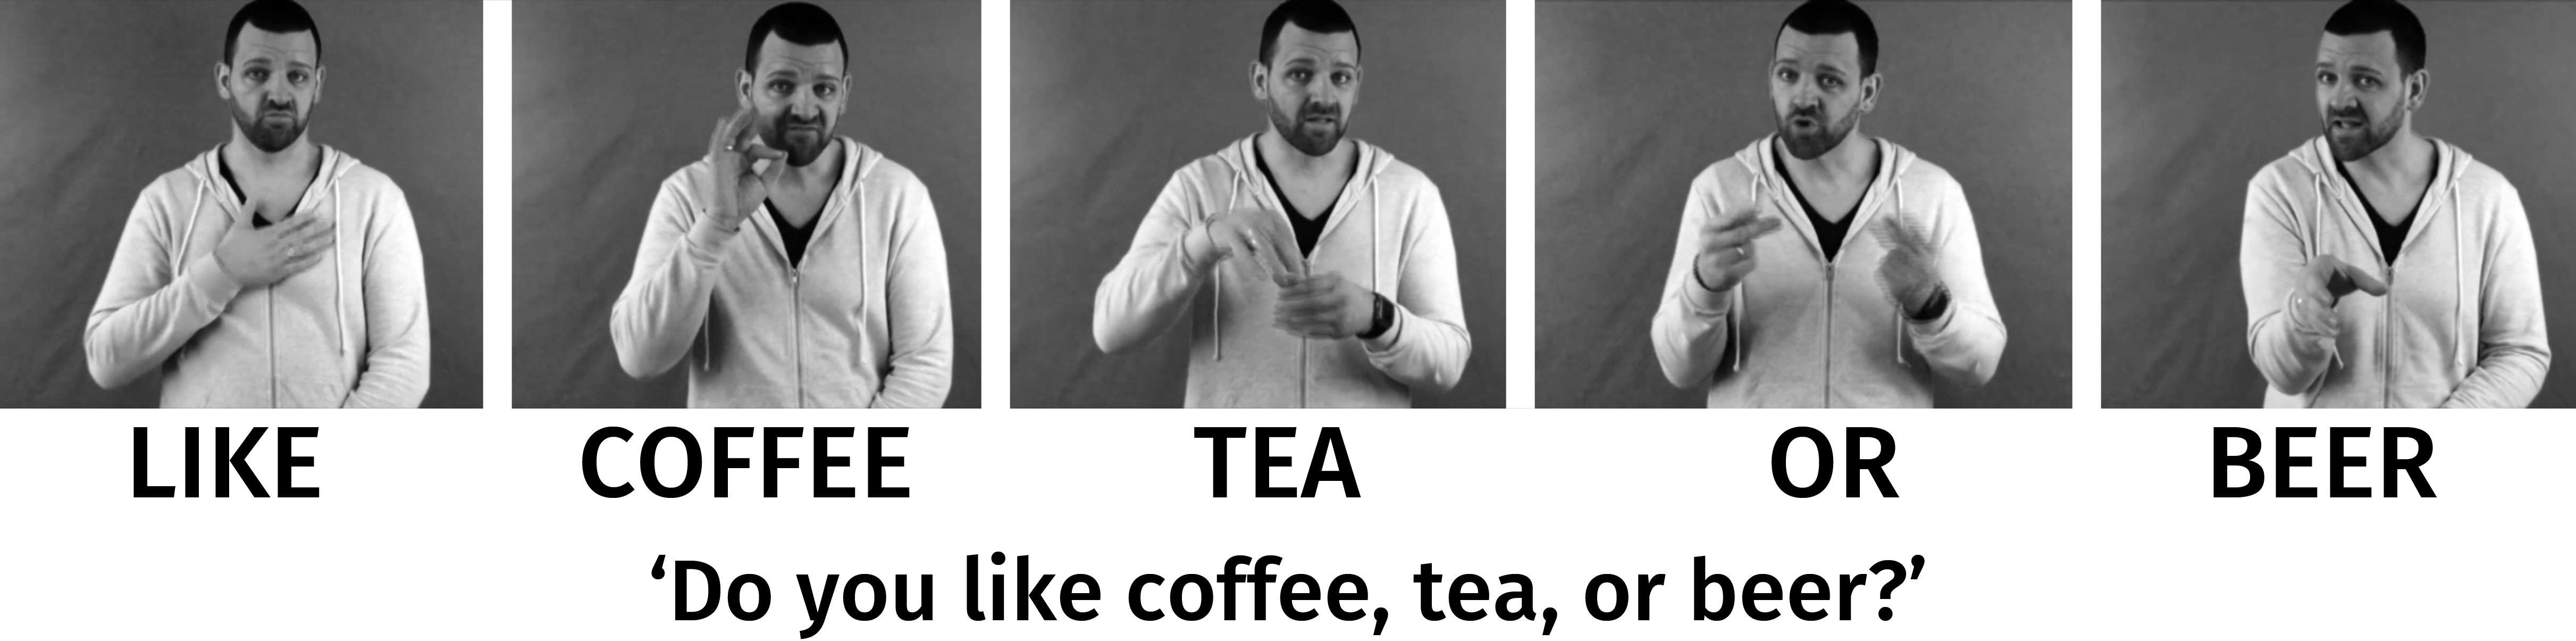
\includegraphics[width=1.0\textwidth]{alternativequestionsw.jpg}
	\caption{The non-manual markings used in alternative interrogatives are the same as in polar interrogatives. Note that the subject is dropped in the example and that the change in word order (VO instead of OV) is not due to the sentence being an alternative question, but is rather related to the verb being volitional.}
	\label{alternativequestion}
\end{figure}

\is{alternative interrogatives|)}


\subsection{Degree questions}
\is{degree interrogatives|(}
%\sub
Degree interrogatives are used to ask a question about the degree of a gradable property (e.g., \textit{How long is your hair?}). There is only scarce mention about this question type in the literature (e.g., \citealt{meier2001result, abrusan2011wh, tiemann2012crosslinguistic}). While questions are traditionally either divided into two major classes, polar and constituent interrogatives, or three classes, polar, constituent, and alternative interrogatives, it is possible that degree questions form a major class of their own. As almost nothing is known about degree questions I will only briefly discuss them here under the header of `other types of interrogatives'.

On the surface, spoken languages often encode degree questions as \textit{wh}-ques\-tions. This is, for example, the case in spoken German which makes use of the \textit{wh}-element \textit{wie} `how', as shown in (\ref{ex:germandegree}). 

\begin{exe}
\ex German \\ \gll {\textit{Wie}} {\textit{lang}} {\textit{sind}} {\textit{deine}} {\textit{Haare}?} \\
{how} {long} {are} {your} {hair} \\
\trans `How long is your hair?' \label{ex:germandegree}
\end{exe} 


\noindent Other languages, in contrast, have their own strategies to express degree questions. In Mandarin Chinese, for example, the degree particle \textit{duo} `many' is used to express degree questions, as shown in (\ref{ex:chinesdegree}).


\begin{exe}
\ex Mandarin \\ \gll {\textit{nide}} {\textit{toufa}} {\textit{you}} {\textit{duo}} {\textit{chang}} \\
{you.\textsc{rel}} {hair} {have} {many} {long} \\
\trans `How long is your hair?' \label{ex:chinesdegree}
\end{exe} 

\noindent The only mention of this question type in the literature on DGS, as far as I am aware, is found in \citet[335]{happ2014vork} who label it `million alternatives questions' as the answer set of alternatives is theoretically infinite \citep{fox2006universal}. DGS has its own strategy to encode this question type. To form a degree question, the signer produces the sign denoting the property in different degrees. This is illustrated in (\ref{ex:millionalternativequestion}). The non-manuals used with degree questions do not differ from those used with polar questions, as shown in Figure (\ref{millionalternativequestions}).

\begin{exe}
\ex \slg[degree]{poss_2 dog big(1) big(2)}
%{\hspace{103pt}degree}  \\
%{$\overline{\textrm{\textsc{poss}\textsubscript{2} \textsc{dog big(1) big(2)}}}$}
\glt `How big is your dog?' \label{ex:millionalternativequestion}
\end{exe}


\begin{figure}[bt]
\centering
	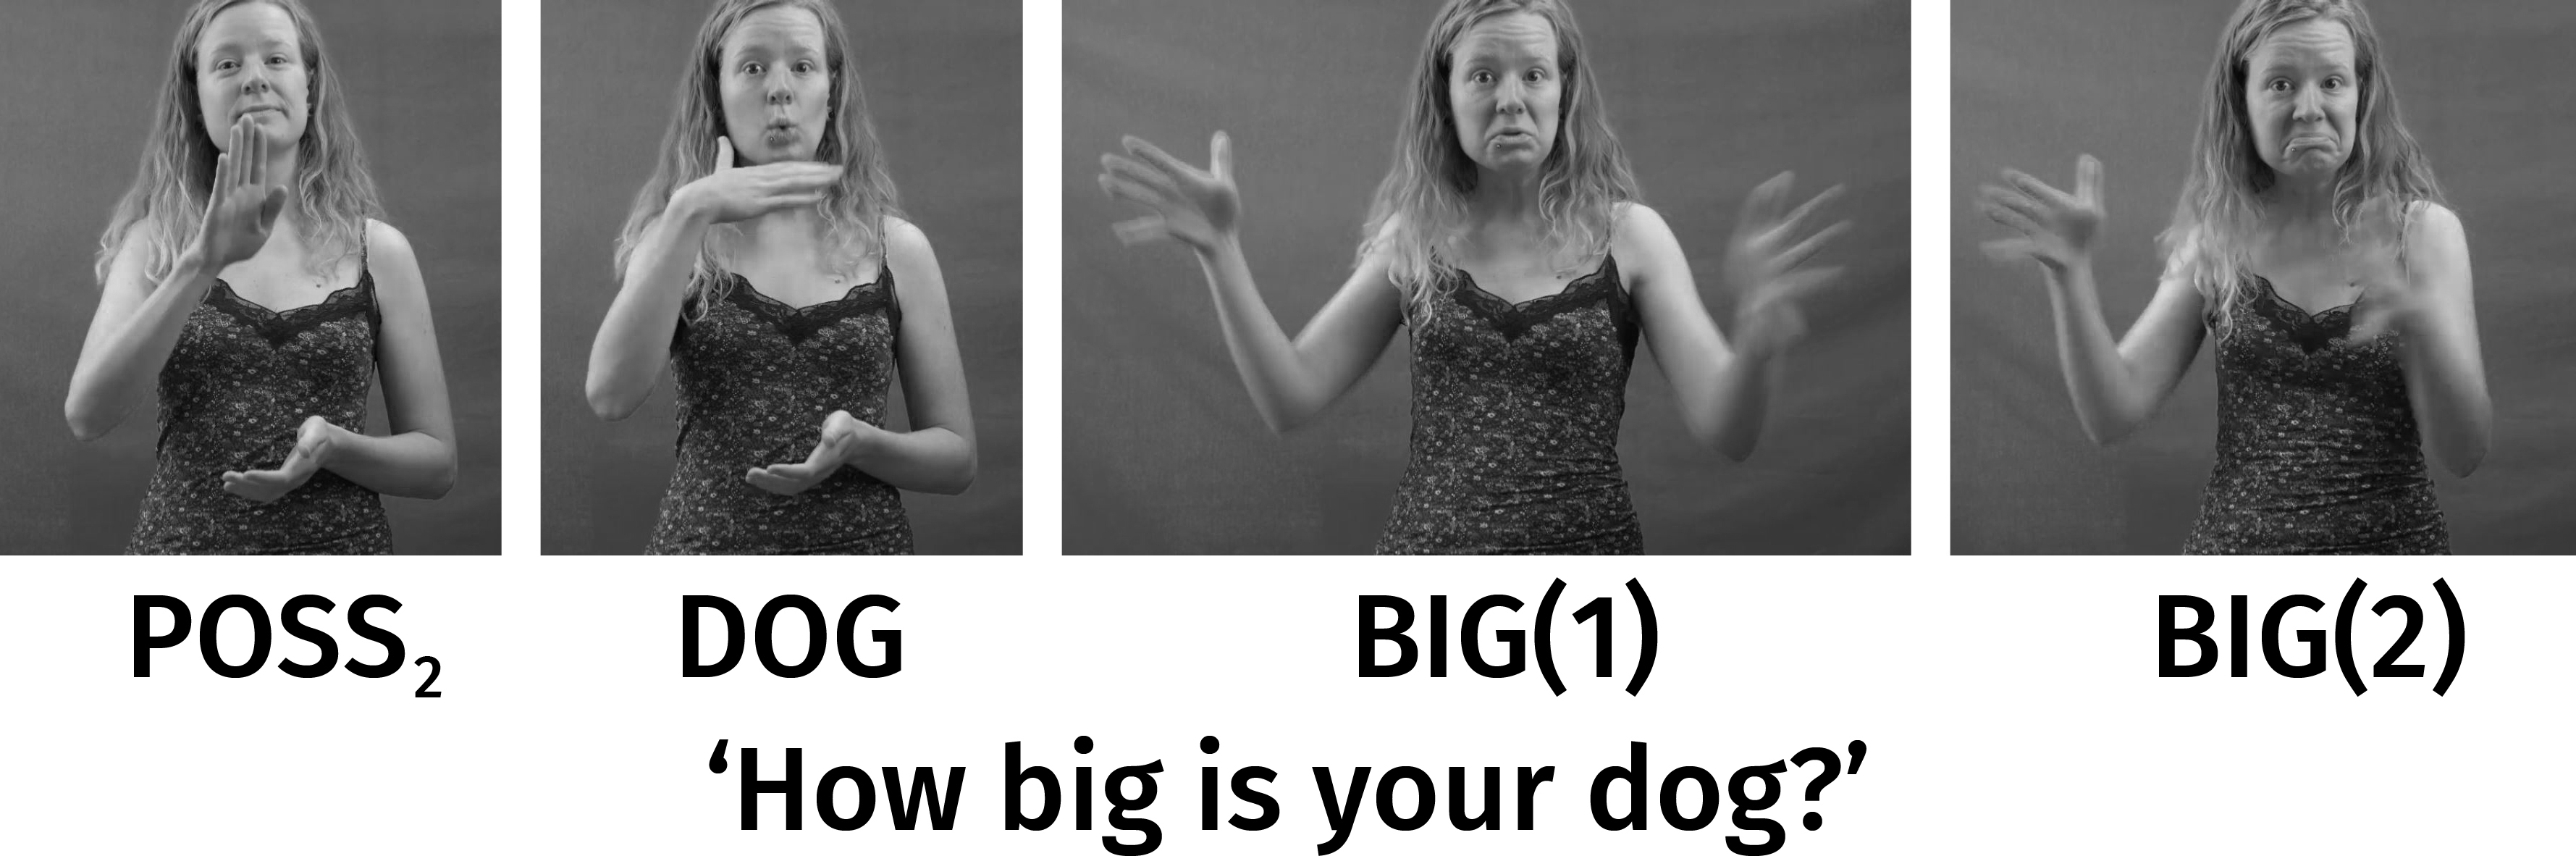
\includegraphics[width=1.0\textwidth]{millionalternativequestionssw.jpg}
	\caption{Example of a degree question in DGS. Note that the signer pulls her mouth angles down towards the end of the sentence. This seems to be an optional (and thus gestural) non-manual expressing that the signer is missing some information.  }
	\label{millionalternativequestions}
\end{figure}

\is{degree interrogatives|)}

\subsection{Tag questions}
\is{tag questions|(}\is{question tag|see{tag question}}
Tag questions, i.e., yes/no interrogatives used when the speaker/signer suddenly becomes uncertain about a proposition s/he felt sure about previously and is seeking the hearer's support along the way, are produced using the tag sign \textsc{right} or its negative pendant \textsc{right-neg}. The non-manuals of a regular polar question and the non-manuals of a tag question are the same (which is expected, as tag questions, in fact, are polar interrogatives). This means that the eyebrows are raised and the head is put forward and tilted. These non-manuals, again, are strongest clause-finally. However, there is a clear pause before the question tag and the tag itself may be accompanied by a head nod. This is illustrated in Figure \ref{tagquestion}.

\begin{figure}[bt]
\centering
	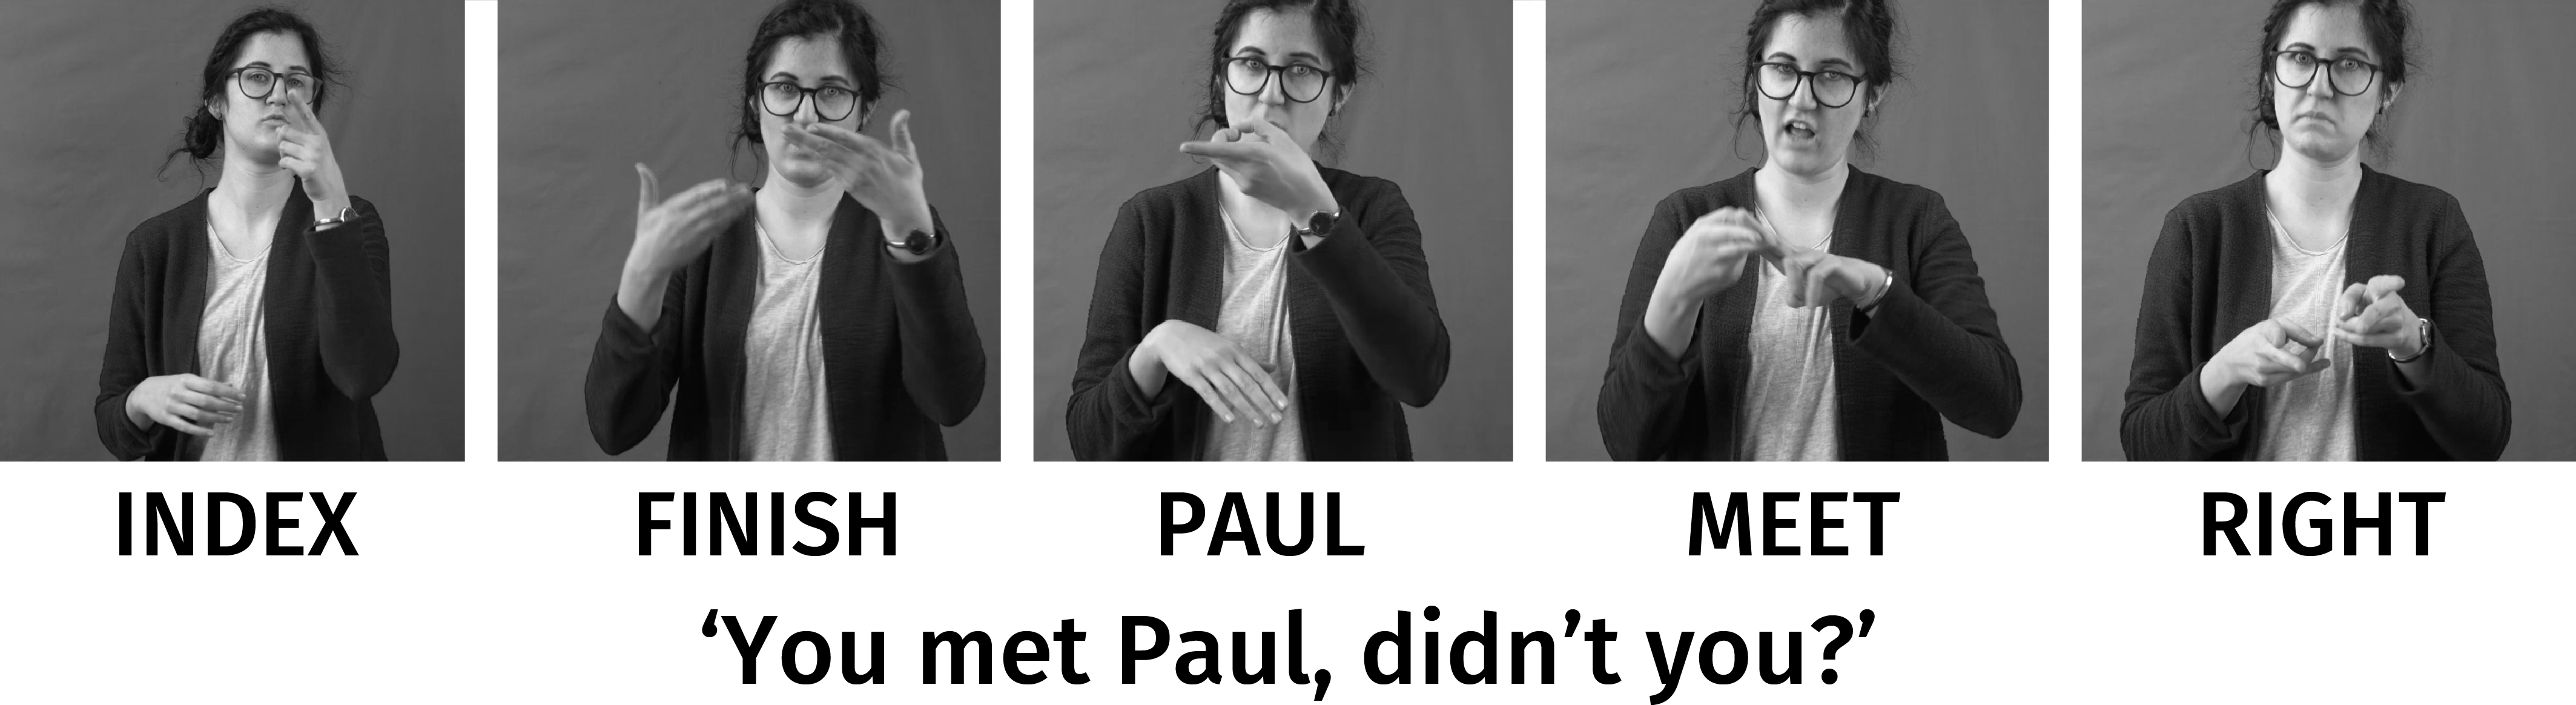
\includegraphics[width=1.0\textwidth]{tagquestionsw.jpg}
	\caption{The non-manuals used in tag question do not differ from polar questions. The tag itself is preceded by a clear intonational break and the question tag is accompanied by a head nod. Note that in this example, the sign \textsc{finish} appears as a perfect marker.}
	\label{tagquestion}
\end{figure}

\is{tag questions|)}


\subsection{Suggestive questions}
\is{suggestive questions|(}
Interrogatives used as suggestions and especially \textit{why-not}-questions are of special interest because this type of interrogative is superficially very similar to \textit{wh}-interrogatives, with the difference that \textit{why-not}-questions are not used as real information-seeking questions. I have found no restrictions as to the landing site of the \textit{wh}-phrase with suggestive questions although the clause-internal position seems to be preferred (i.e., the \textit{wh}-sign is left \textit{in-situ}). A typical example looks like the one in (\ref{ex:suggquest}). 

\begin{exe}
\ex \slg[sugg-wh]{today why not vegetarian cook}
%{\hspace{158pt}sugg-wh}  \\
%{$\overline{\textrm{\textsc{today why not vegetarian cook}}}$}
\glt `Why don't we cook something vegetarian today?' \label{ex:suggquest}
\end{exe}

\noindent The most important difference between real information-seeking questions and suggestive questions is of non-manual nature. As shown in Figure \ref{suggquest}, lowered and squinted eyebrows as the common markers of \textit{wh}-questions are nearly absent in suggestive questions. Additionally, the eyes are more open. This observation supports the idea that the eyebrows play a major role in clause-typing. 

\begin{figure}[bt]
\centering
	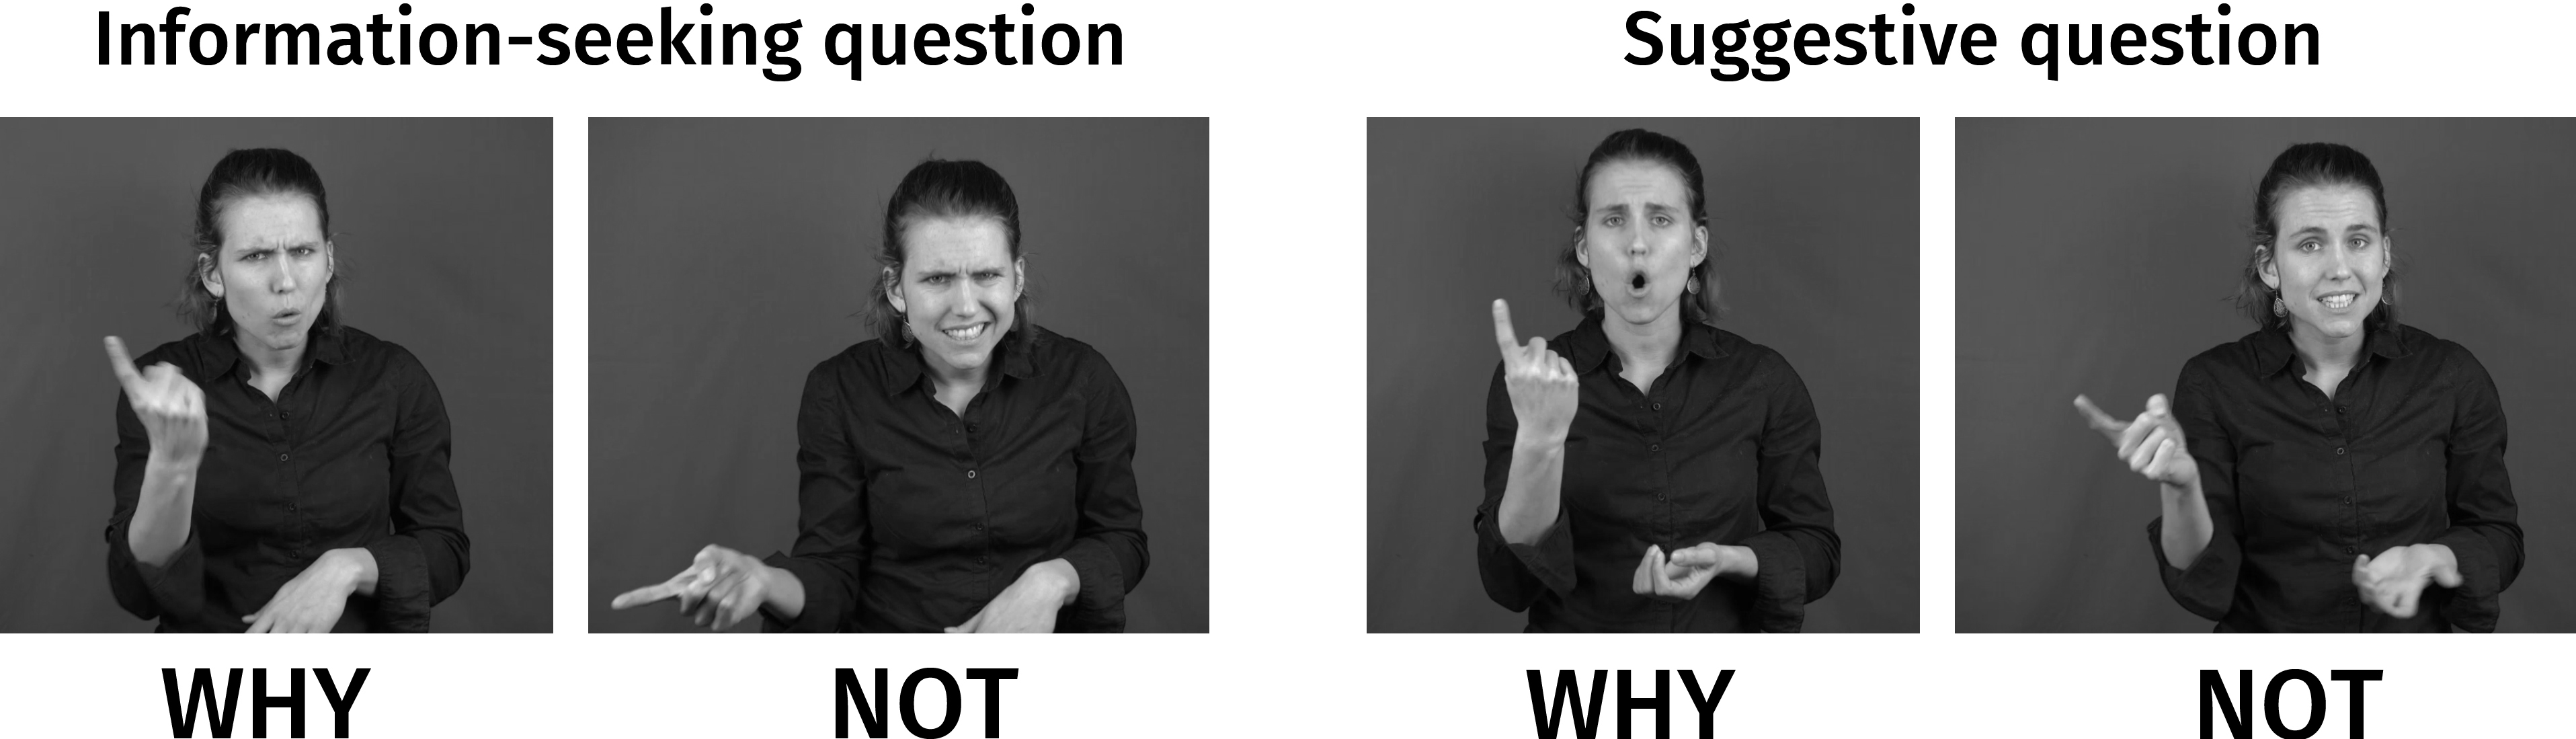
\includegraphics[width=1.0\textwidth]{suggquestsw.jpg}
	\caption{Non-manual differences between information-seeking and suggestive questions. }
	\label{suggquest}
\end{figure}



\is{suggestive questions|)}

\subsection{Rhetorical questions}\label{rhetq}
\is{rhetorical question|(}
I will now turn to the discussion of rhetorical questions. A question is interpreted as being rhetorical when the answer to the question is in the common ground of the interlocutors \citep{caponigro2007rhetorical}. In other words, the hearer needs to be able to reconstruct the answer to the question \citep{truckenbrodt2004strukturbedeutung}. Rhetorical questions can be realized as polar or constituent interrogatives. Examples, including the re-constructable answers, are given in (\ref{rhetquestspoken}). 

\begin{exe}
\ex\label{rhetquestspoken}\begin{xlist}
\ex Do you want to miss this chance? \\
\textasciitilde You do not want to miss this chance. \label{polarrhet}
\ex Who likes rocket salad? \\
\textasciitilde Nobody likes rocket salad. \label{constituentrhet}
\end{xlist}
\end{exe} 

\noindent Note that the rhetorical questions in (\ref{rhetquestspoken}) are used to make statements. There are, however, other speech acts that can be performed with rhetorical questions, e.g.,  accusations (\textit{Why do you always act like a child?}). 

The question of how rhetorical questions are formed in sign language has not received much attention in previous research. Most of the research concerns question-answer pairs, such as the one from \citet[138]{baker1980american} in (\ref{ex:bakercokely}) (with `rq' meaning rhetorical question). I will not discuss this use as it may be better analyzed as an instance of pseudo-clefting (e.g., \citealt{wilbur1996evidence}; see also the discussion starting from page \pageref{pseudocleeeeefts}).%\footnote{Thus, the translation of the example in (\ref{ex:bakercokely}) would rather be something like: `Why the woman died is because she refused to eat.'}(note that the structures discussed here are `real' rhetorical questions and not pseudo-clefts as discussed starting from Page \pageref{pseudocleeeeefts} which are also sometimes called `rhetorical' in the literature)

\begin{exe}
\ex American Sign Language\\ \slg{woman die,} \slg[rq]{why,} \slg{refuse eat}
%{} {\hspace{86pt}rq} {} \\
%{\textsc{woman die,}} {$\overline{\textrm{\textsc{why}}}$,} {\textsc{refuse eat}}
\glt `This woman died, because she refused to eat.' \label{ex:bakercokely} 
\end{exe}

\noindent Instead, I will briefly describe how real rhetorical questions are formed in DGS. Rhetorical questions are of special interest concerning the non-manual markers used in DGS questions. In Section \ref{polarinterrogativesdgs} and Section \ref{whinterrogativedgs}, I have argued that each of the three non-manual markers in DGS interrogatives has a meaning on its own. To be more precise, I claimed that raising the eyebrows is the general marker of a polar question and lowering the eyebrows is used to mark constituent interrogatives, that putting the head forward signals that the signer is expecting an answer/reaction, and that tilting the head siedways is used to express epistemic commitment (see also Section \ref{perhapsmoodirrealis}). 

These claims can be tested with rhetorical questions. As rhetorical questions are still questions, we would expect the eyebrow marking to be present in both polar and constituent rhetorical questions. As the asker knows the (expected) answer in a rhetorical question we would expect putting the head forward to be absent. The same prediction can be made for tilting the head sideways as there should be no epistemic insecurity about the proposition expressed. 

\citet[333]{happ2014vork} discuss rhetorical constituent interrogatives in DGS and claim that they are marked by raised instead of lowered eyebrows. However, they define rhetorical questions as questions in which the person who asks the question knows the answer and only give examples from classroom contexts in which a teacher asks a question. As a teacher asking an examination question does know the answer, this type of question falls under their definition.

Educational questions asked in examination contexts are, although they are not to be considered as real rhetorical questions, of special interest as the circumstances in which they are being used are highly interesting. With an educational question, the asker knows the answer, but is still expecting an answer. We thus would expect the head being put forward, but expect the sideways tilt being absent. As shown in Figure \ref{educational}, this is indeed the case. With the educational constituent question shown in the figure, the signer raises her eyebrows, as described by \citet{happ2014vork}. As expected, the signer's head is straight, but put forward towards the end of the clause in the figure.\footnote{It could be speculated that educational constituent interrogatives are a special kind of alternative question with the alternatives being the correct and the incorrect answers. This way, the raised eyebrows can be explained.}

\begin{figure}[bt]
\centering
	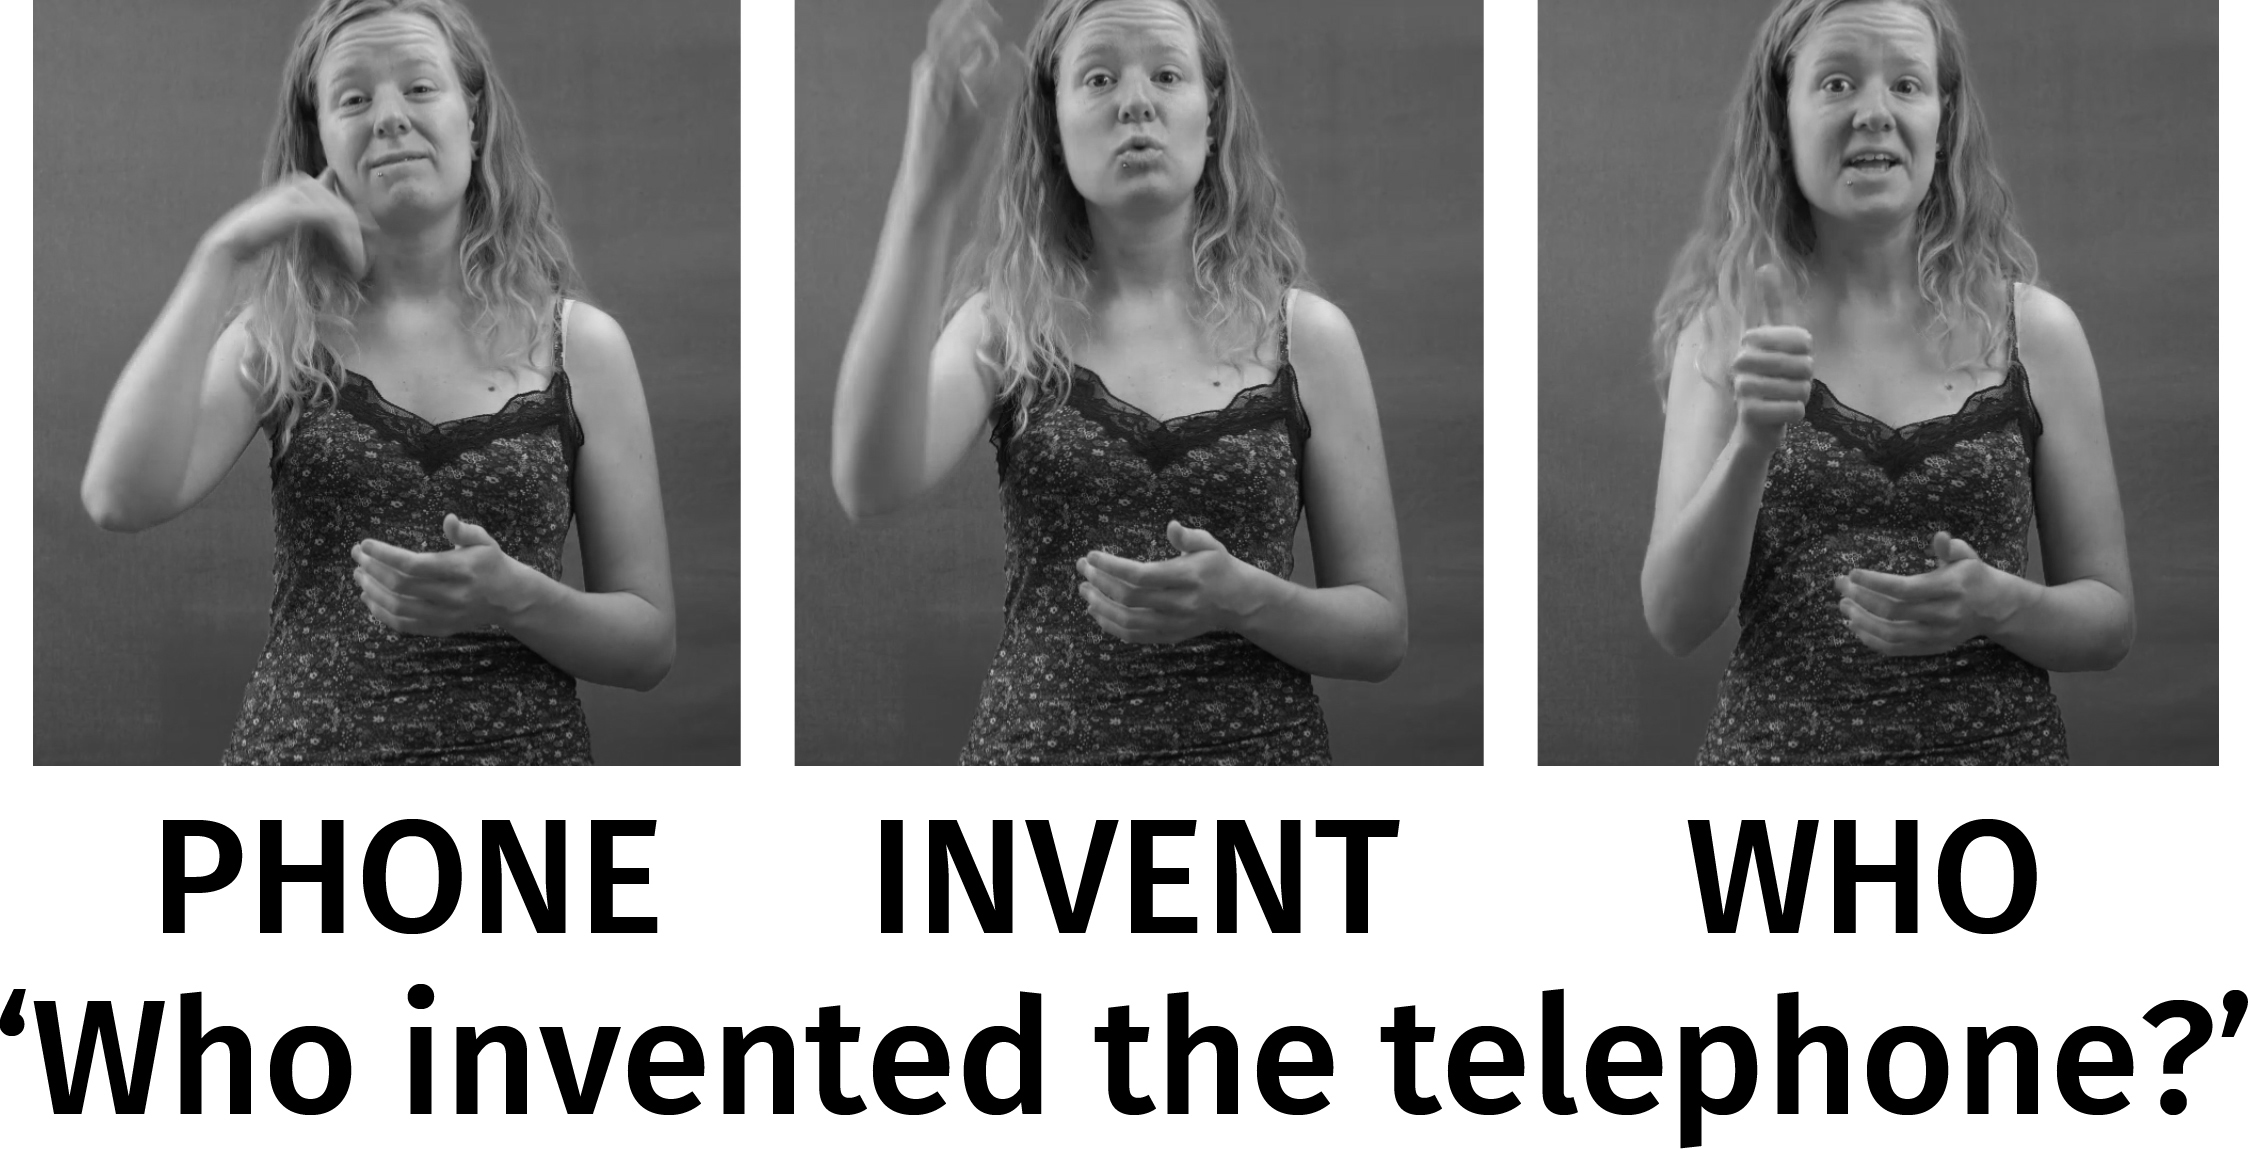
\includegraphics[width=1.0\textwidth]{educationalsw.jpg}
	\caption{Educational constituent interrogatives can be accompanied by raised instead of lowered eye-brows.}
	\label{educational}
\end{figure}

Other types of rhetorical questions, however, receive different eyebrow markings and I argue that there is no uniform marking of rhetorical questions in DGS in the sense that there is one non-manual marker for this question type. In many cases, rhetorical questions are marked by furrowed brows. This is especially true for accusations, as shown in Figure \ref{accusation}. As can be seen from the example, the signer leans back towards the end of the sentence to signal that she is not sympathetic with the behavior of the addressee -- this non-manual, however, is not part of the rhetorical question, but of the speech act of accusing.

\begin{figure}[bt]
\centering
	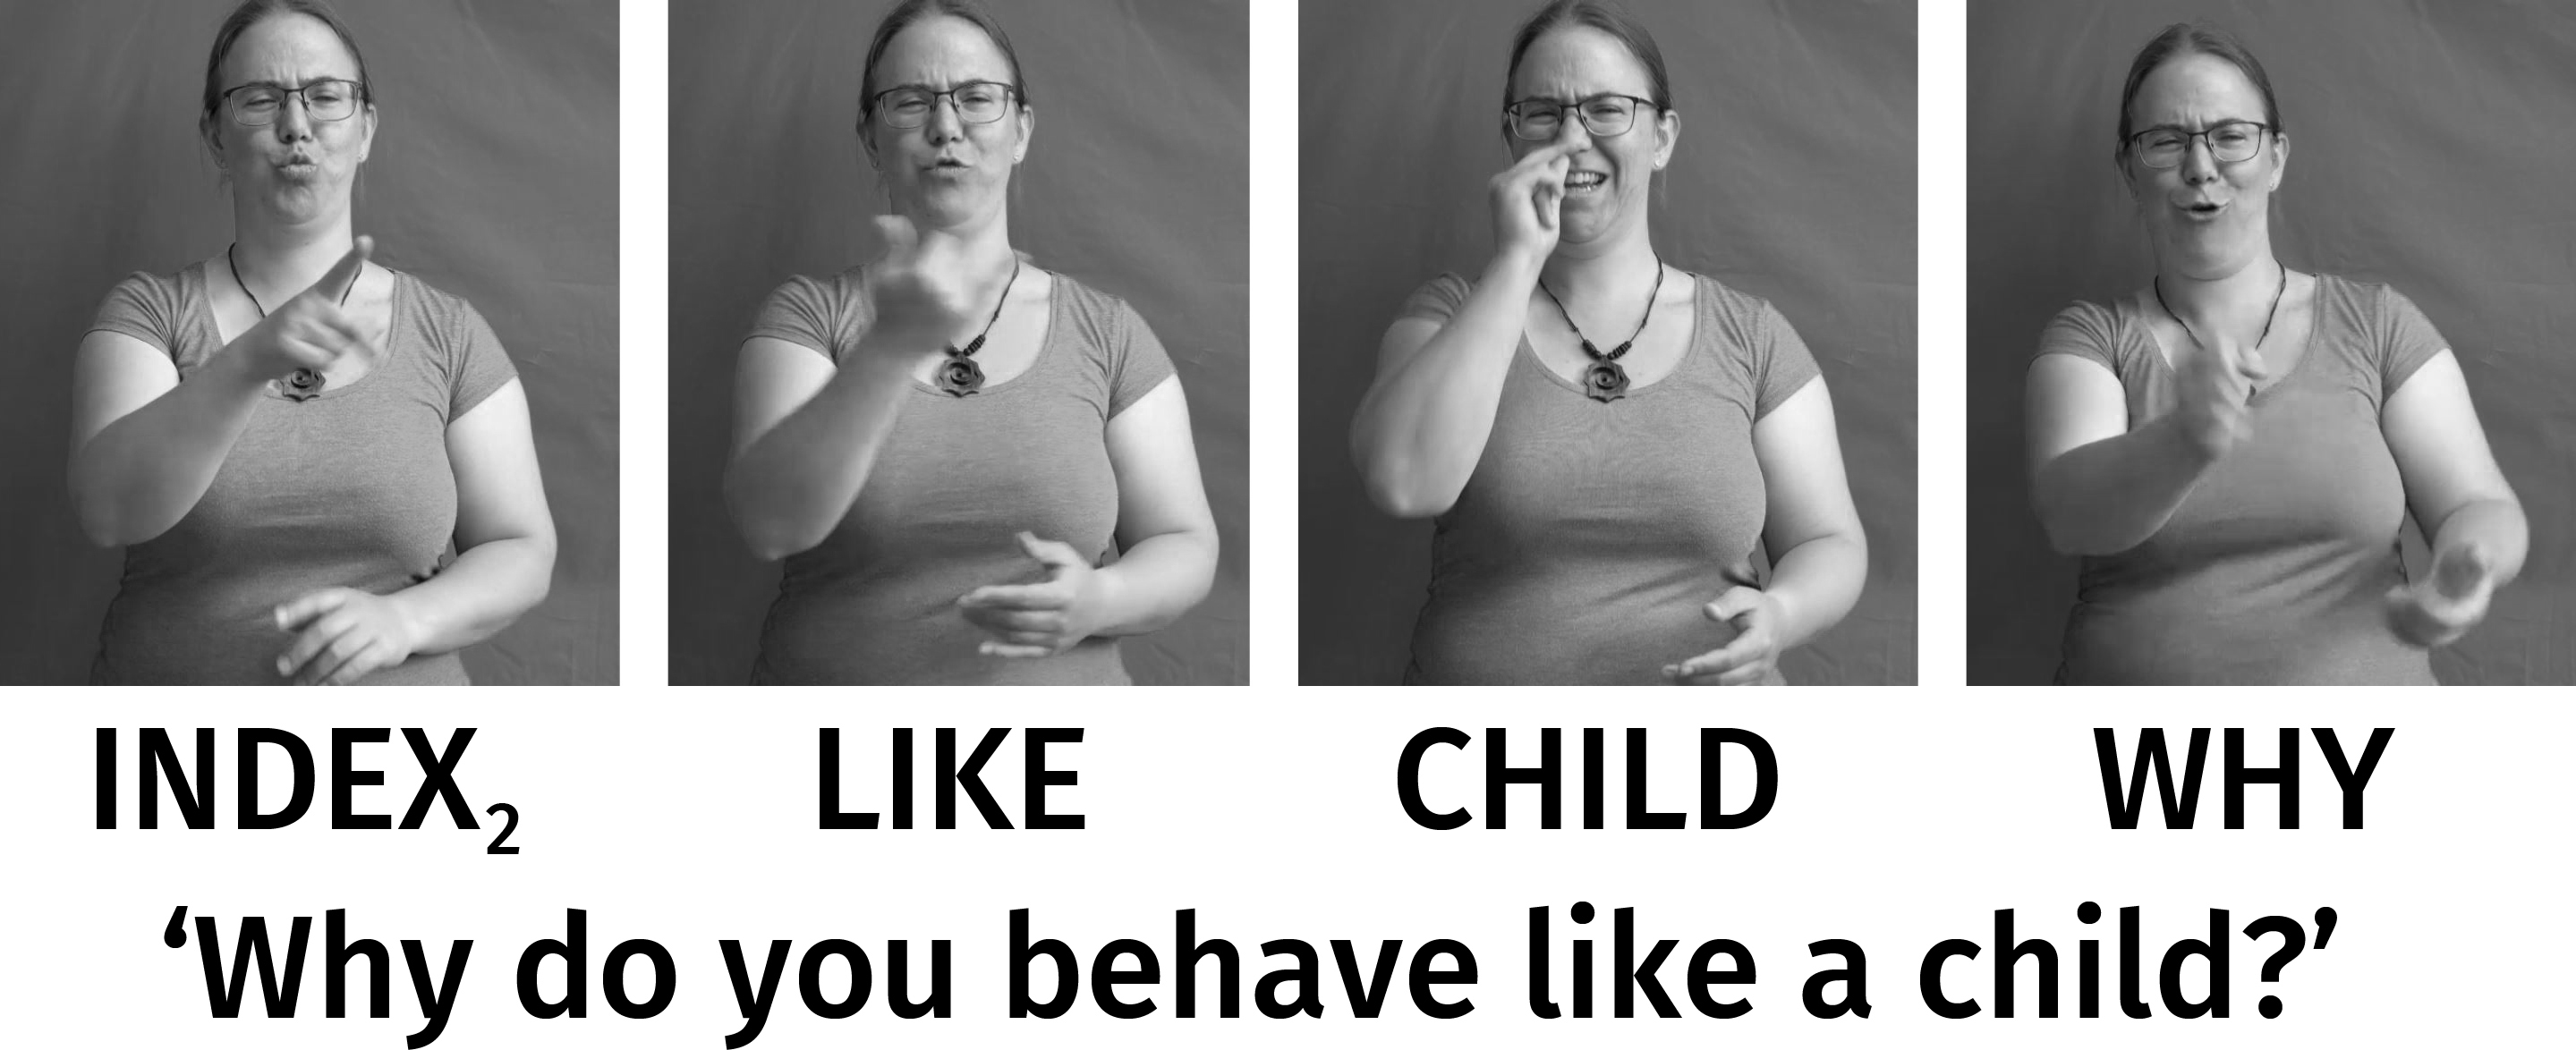
\includegraphics[width=1.0\textwidth]{accusationsw.jpg}
	\caption{Rhetorical questions used as accusations receive furrowed brows.}
	\label{accusation}
\end{figure}

The non-manuals for rhetorical questions that are used as statements are subject to variation. It seems as if rhetorical questions with negative re-constructable answers receive a brow-furrow. This is illustrated for a rhetorical content and a rhetorical polar question in Figure \ref{rhetorical}. Note that in both cases, the head is in a straight position and not put forward -- as the signer does know the answer and does not expect a response from the addressee. Additionally, rhetorical questions can be followed by a palm-up gesture, as shown in the figures. Note that the impression that the signer tilts her head sidewards comes from the fact that the palm-up gesture is accompanied by a head-shake (to indicate that the expected answer is no). 

\begin{figure}[bt]
\centering
	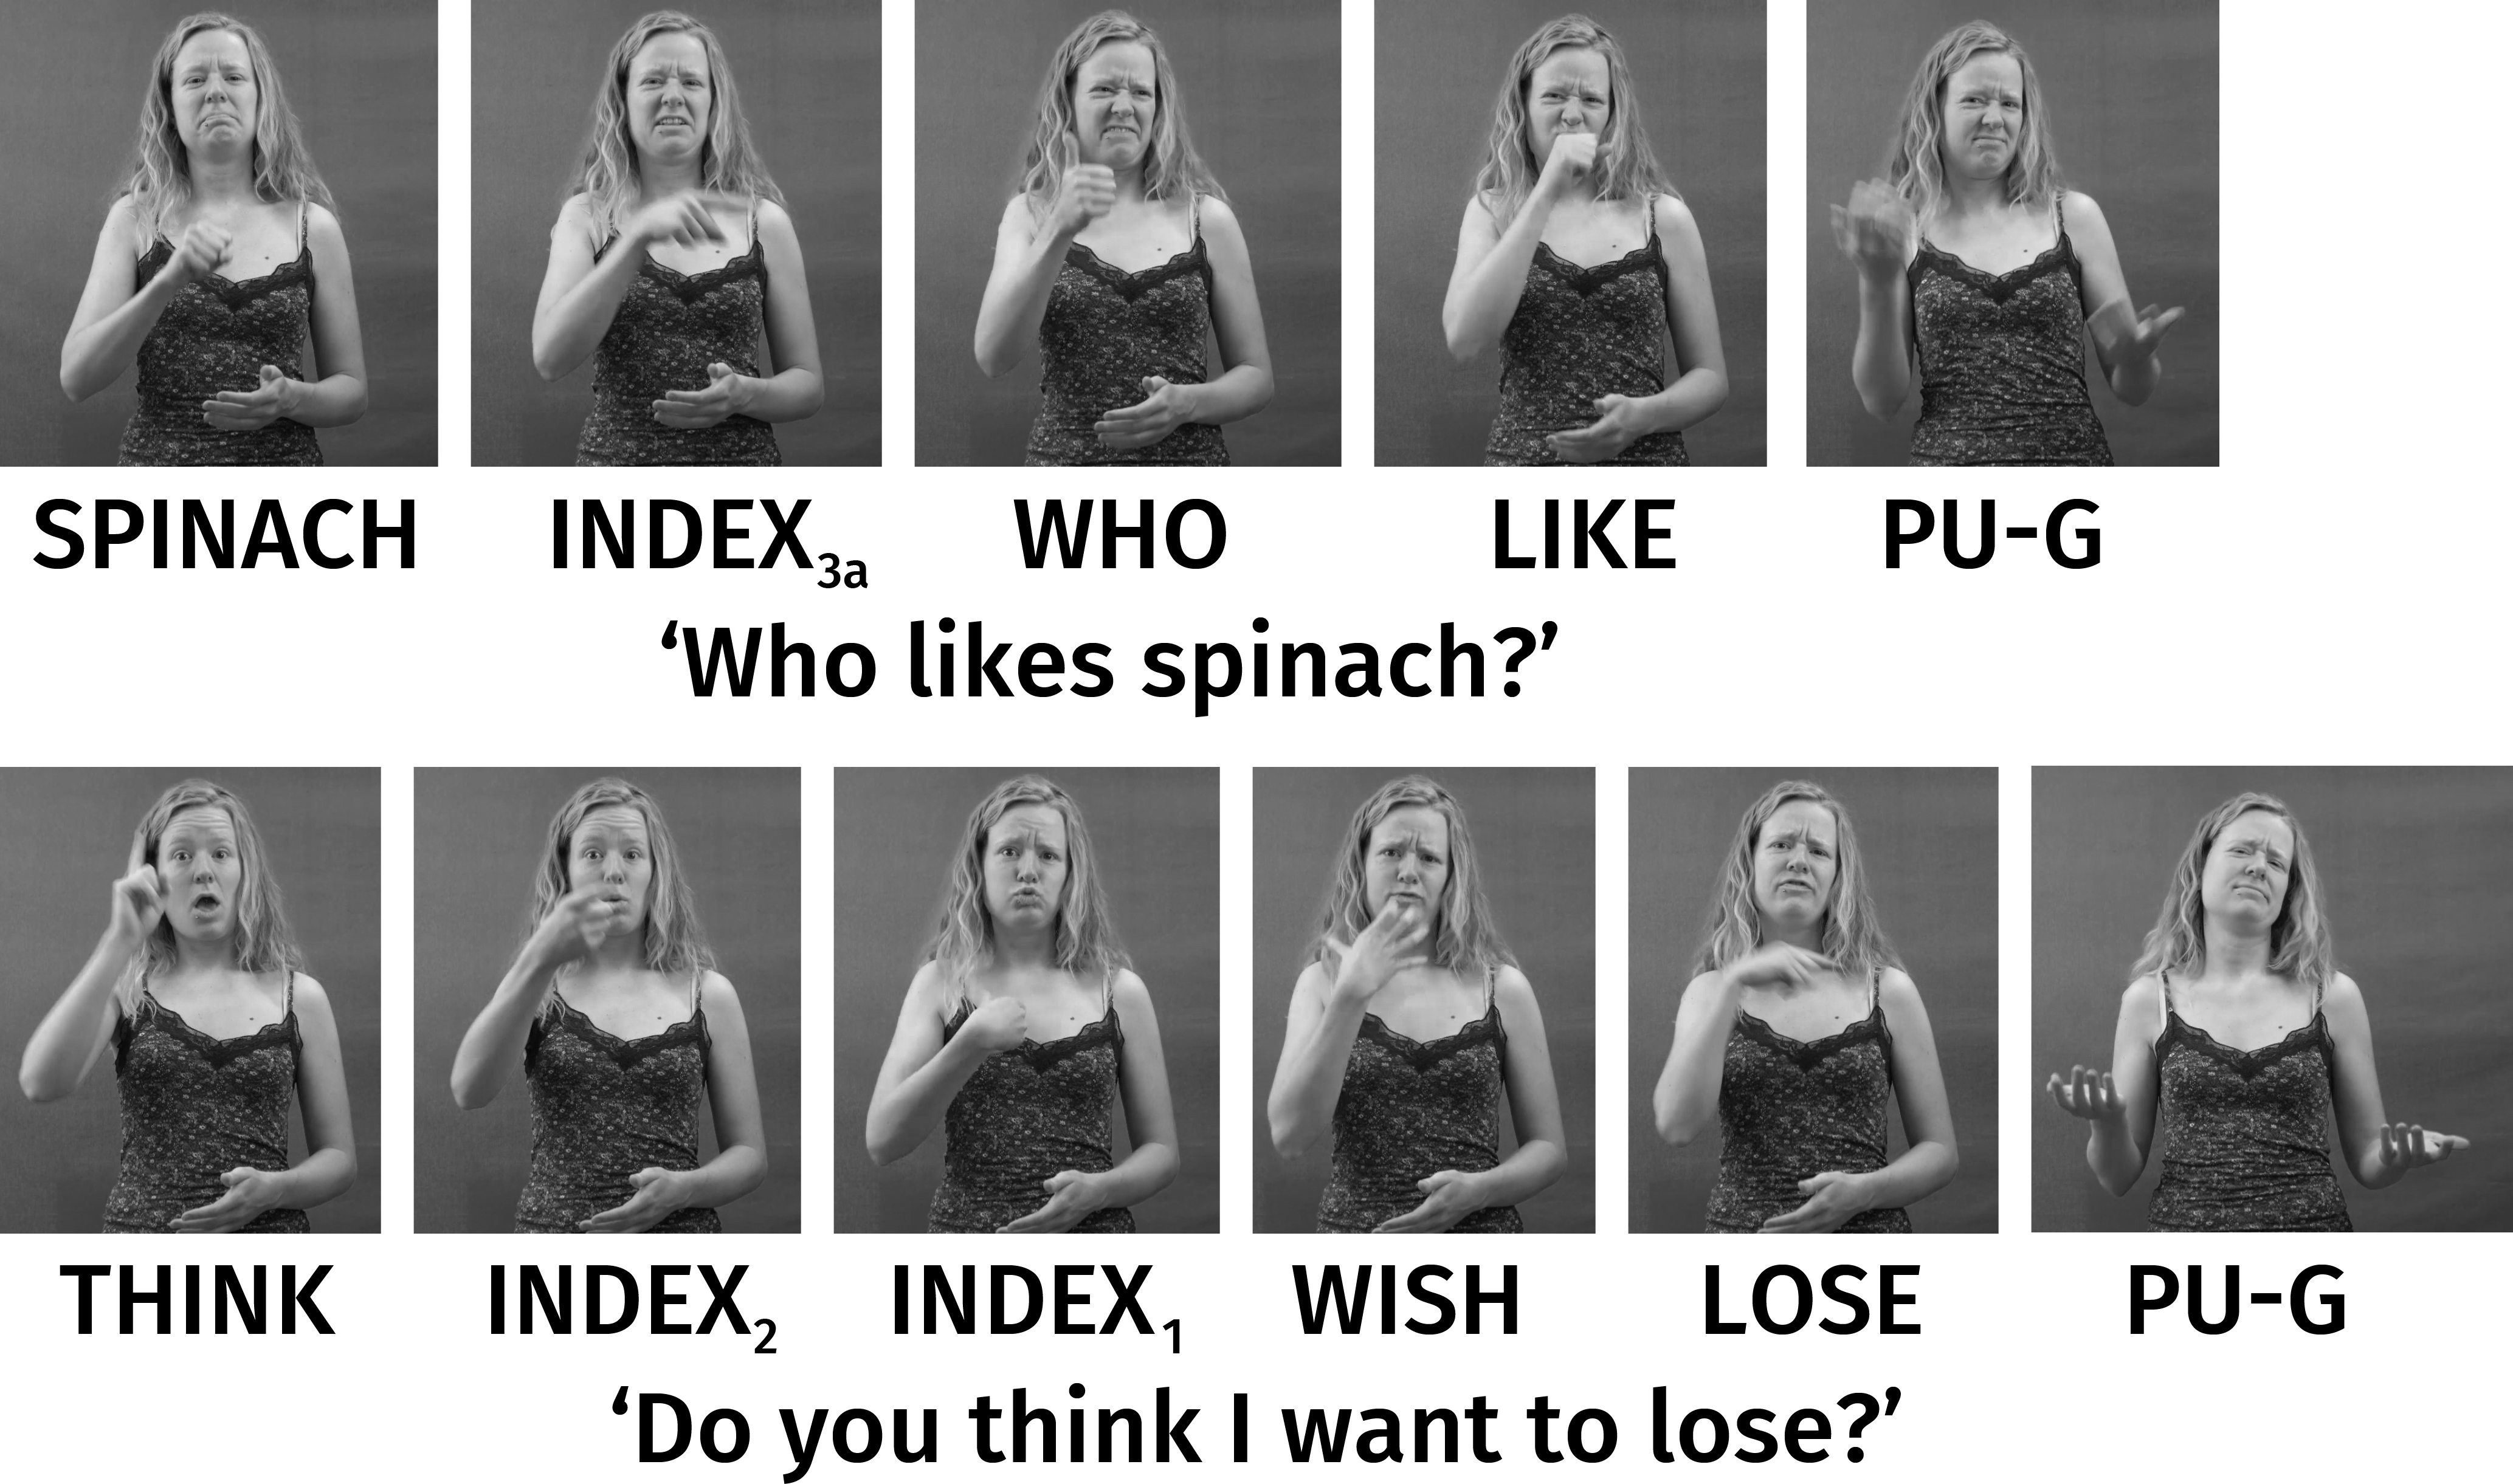
\includegraphics[width=1.0\textwidth]{rhetoricalsw.jpg}
	\caption{Rhetorical questions expressing negative statements are marked with furrowed brows.}
	\label{rhetorical}
\end{figure}
%\clearpage
Rhetorical questions used as statements with positive re-constructable answers seem to receive eyebrow raise. This is shown using the example \textit{Don't we all want to be loved?} (triggering the positive re-constructable answer `Yes, we all want to be loved'), in Figure \ref{rhetlove}. Again, the head is held straight and not tilted to the side. 

\begin{figure}[bt]
\centering
	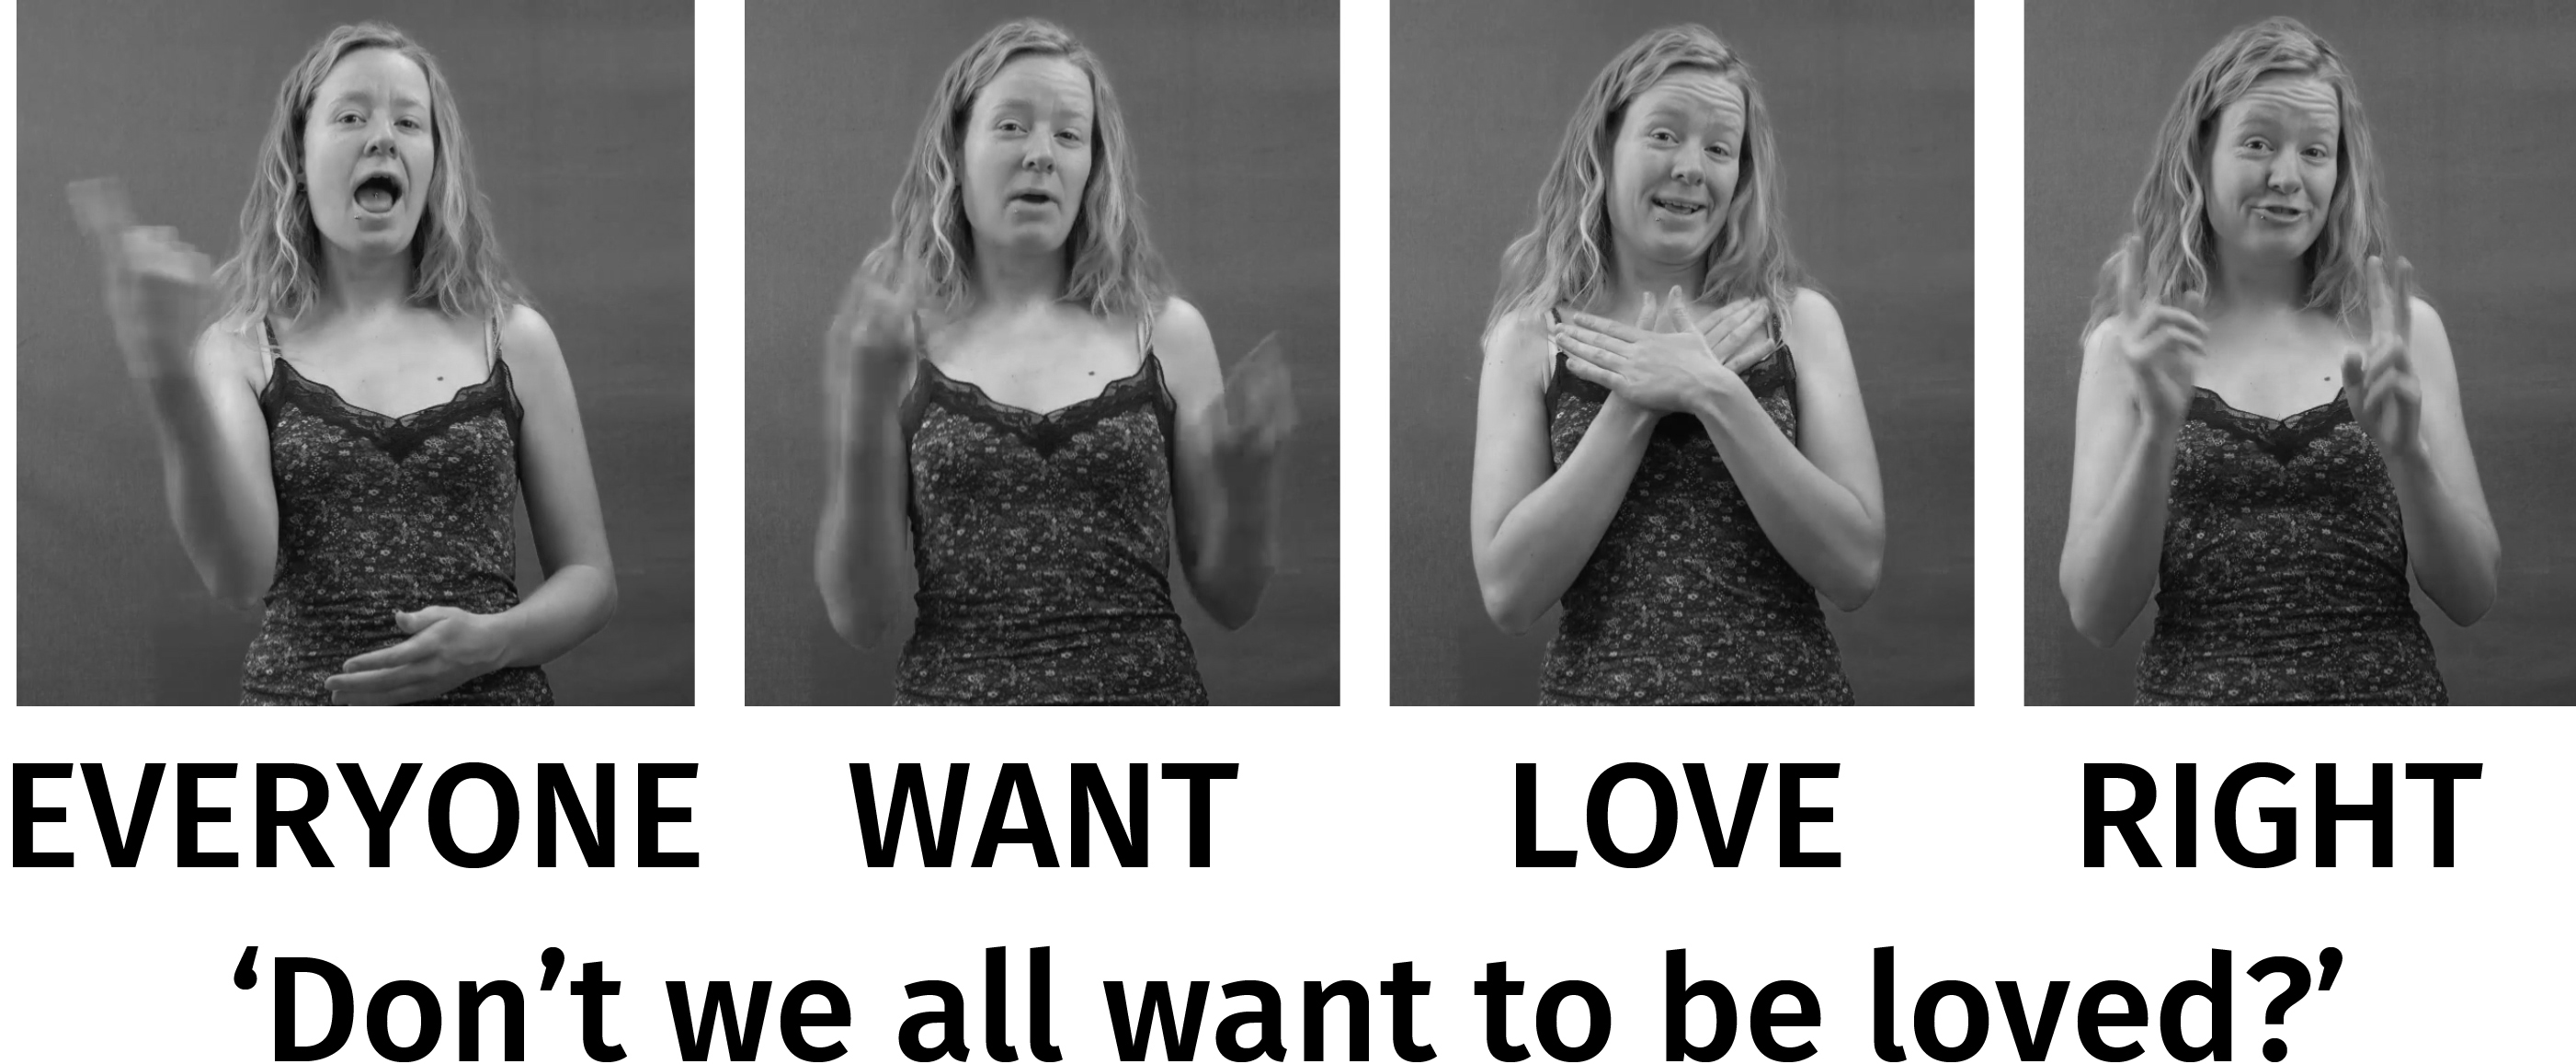
\includegraphics[width=1.0\textwidth]{rhetlovesw.jpg}
	\caption{Rhetorical questions expressing positive statements are marked with raised brows.}
	\label{rhetlove}
\end{figure}

Taken together, rhetorical questions receive non-manual markings with the eyebrows. The exact non-manuals depend on the answer to be reconstructed. 

\is{rhetorical question|)}

\section{Imperatives}\label{generalsectionimperatives}
\is{imperatives|(}
As in the previous sections, I will begin this section with a discussion of the general features of the phenomenon in spoken languages, followed by an overview over the sign language literature. Finally, I will go through the DGS data. I will show that the main marker of imperatives are the eyebrows, again with an intensity peak towards the end of the clause. In summary, the syntactic analysis of imperatives presented will not differ much from polar interrogatives: I assume that with imperatives, feature checking in a high CP projection takes place, triggering the non-manual markings -- the responsible head is either right-headed or left-headed with the whole clause being moved to a left-branching specifier. Besides the non-manuals, I will briefly discuss subject drop, the agreement behavior of verbs in imperative sentences, and negation in imperatives. 

\subsection{General overview}
Imperative sentences are sentences that are (typically) used for the communicative function of an order or request, i.e. the speaker/signer wants the addressee to carry out an action. An often cited definition of the prototypical meaning of an imperative is by \citet[212]{schmerling1982imperatives} who characterizes an imperative as ``an attempt to bring about a state of affairs in which the proposition expressed by the imperative is true''. This, however, downplays the importance of the addressee \citep[31]{van2007imperatives}. Although it covers orders, requests, and wishes, it does not say anything about who is addressed and if the attempt is realistic or not. It covers, for example, optatives of the sort \textit{May you live 100 years} that should not be covered by the term imperative. Additionally, this definition would cover promises such as \textit{In the future, I will never go to bed so late!} The missing part of Schmerling's definition is that the one who uses an imperative has the intention that the addressee adds the proposition expressed by the imperative to his/her to-do list in \citeauthor{portner2004semantics}'s (\citeyear{portner2004semantics}) terminology. Summarizing Generative analysis of imperatives, \citet[32]{van2007imperatives} concludes that the core meaning of an imperative is to get the ``addressee to bring about a state of affairs''. 

\newpage 
The prototypical directive is a command \citep[1--2]{aikhenval2010imp} although imperatives can be used for a variety of other directive speech acts as several authors stress. \citet[213]{clark1996using}, for example, notes:

\begin{quote}
A simple imperative like ``Sit here,'' for instance could be used as a command, request, offer, advisory or exhortation, depending on the context, as is shown by the following potential responses: ``Yes, sir'' (command), ``Okay'' (request), ``No thanks'' (offer), ``What a good idea'' (advisory), ``Thank you'' (exhortation).
\end{quote}

\noindent As noted already in Section \ref{sec:speechacts} (see page \pageref{threesources}) we need to be careful with the notions of sentence types, sentence mood, and the force of an utterance. The force of an utterance is inferred by a hearer from a combination of three sources: the context, the mood as encoded by syntax and the proposition expressed. Although imperatives like \textit{Sit here!}, \textit{Open the window!}, or \textit{Lie on the floor!} can be understood as a command, request, etc. in different contexts, without politeness markers it is understood as a command when no context is present and not as a request, offer, advisory, or exhoration (although it is often stressed the imperative mood is more flexible as it can express more speech-acts than other sentence moods, e.g., \citealt{portner2004semantics}; \citealt{kaufmann2012terpreting}).

Imperative sentences show a set of cross-linguistically stable properties. In the following I will briefly discuss three of these properties as they are either of interest when it comes to sign languages or are telling when it comes to the syntax of imperatives: (i) subject drop, (ii) the minimal verbal morphology found in imperatives, and (iii) the behavior of negation in imperatives. 

The first property of imperative sentences I will elaborate on is that they cross-linguistically allow for subject-drop -- even in languages that otherwise do not allow null-subjects (e.g., \citealt{alcazar2014syntax}). Broadly speaking, that the subject can be dropped in imperatives is due to the fact that the subject of an imperative is the addressee who is, under normal circumstances, present in the context of utterance. Although it seems as if there is no language that does not have the option for a non-overt subject in imperatives (e.g., \citealt{sadock1985speech}) there are good reasons to believe that imperatives nevertheless have a non-overt second person subject (\citealt{zwicky1988subject, potsdam1996syntactic} and the summary in \citealt[33--34]{van2007imperatives}). The major piece of empirical evidence for this assumption is that it is possible to bind a reflexive pronoun, as in (\ref{bindinga}).

\begin{exe}
\ex Introduce yourself! \label{bindinga}
\end{exe} 


\newpage 
\noindent As a reflexive pronoun like \textit{yourself} in (\ref{bindinga}) always needs to be bound we need to ask what its binder is. The only possibility here is that it is a second person subject referring to the addressee.

The second property of imperatives I briefly want to discuss is the (cross-lingustically stable) minimal verb morphology. Although there is a wide range of languages that employ special inflections to mark imperatives -- even including \is{reduplication}reduplications, as, for example, in Hopi \citep{benett1981} -- there is a strong tendency to use as minimal inflection as possible (just the verb root in the extreme case). \citet[172--173]{sadock1985speech}, for example, report that approximately half of their sample of 23 languages make use of no affixes at all. A related property of imperatives that has been noted to be cross-linguistically stable is the lack of tense-marking (e.g., \citealt{sadock1985speech}).

From the fact that many languages only show minimal verbal morphology in imperatives and the fact that tense-marking seems to be absent, many authors concluded that the structural make-up of imperatives is somehow impoverished. This is in line with the observation that it is not possible to embed imperatives \citep[78]{katz1964theory} and that there seems to be no language with imperative complementizers \citep[281]{konig2007speech}. However, it is not exactly clear which structures are missing in imperatives. For some authors, the TP is missing in imperatives (e.g., \citealt{zanuttini1991syntactic}) and for others it is FinP (e.g., \citealt{platzack1998subject}). Against the assumption that imperatives lack a TP altogether, \citet{jensen2007favour} argued that the TP encodes the time of the utterance in this sentence type. On her account, it is the CP that is missing in imperatives. Yet other accounts assume that the TP/IP and the CP are fused into one projection in imperatives (e.g., \citealt{wratil2005syntax}).

Thus, there is general agreement on the impoverished syntax of imperatives, but not on its exact nature. However, most authors agree on the idea that there has to be an imperative sentence mood feature in the C domain (e.g., \citealt{rivero1995imperatives, zanuttini1997negation, platzack1998subject, potsdam2007analysing}), although there is no agreement on its exact position. The most natural assumption, at least in my mind, is to assume an imperative projection that should be understood as an analogon to the InterP (i.e., an ImpP). 

The third property I want to discuss briefly is the behavior of negative imperatives. Cross-linguistically there seem to be three strategies. Some languages negate imperatives just as other sentence types, some languages use different negators, and others cannot use imperative verb morphology in negated imperatives. 

\newpage
An example of the first class of languages is German. Thus, German negates imperatives in the same way as other sentence types as illustrated in (\ref{negimperativegerman}). 

\begin{exe}
\ex German\label{negimperativegerman}
\begin{xlist}
\ex {\gll {Ich} {esse} {das} {nicht.}\\
{I} {eat.\textsc{2sg}} {that} {not} \\
\trans `I don't eat that.' \label{negimperativegermabbbbaaa} \hfill\textit{Negative declarative} }
\ex {\gll {Iss} {das!}\\
{eat.\textsc{imp.sg}} {that} \\
\trans `Eat this!' \label{negimperativegermab} \hfill\textit{Imperative} }
\ex {\gll {Iss} {das} {nicht!}\\
{eat.\textsc{imp.sg}} {that} {not} \\
\trans `Don't eat this!' \label{negimperativegermac} \hfill\textit{Negative imperative} }
\end{xlist}
\end{exe}

\noindent The German examples show that in this language, declaratives are negated by the use of \textit{nicht} (\ref{negimperativegermabbbbaaa}). The same particle is used to negate imperatives, as shown by the non-negated (\ref{negimperativegermab}) and the negated (\ref{negimperativegermac}) imperatives. Thus German uses the same negation strategy in imperatives as in other sentence types.% it is no problem to use the regular negator \textit{nicht} with an imperative verb form. 

Languages of the second class use different negators in imperatives than in other sentence types. Languages of this class are the American Indian language Yokuts, Old Greek, or Latin. This strategy is exemplified for Latin in (\ref{negimplat}).

\begin{exe}
\ex Latin\label{negimplat}
\begin{xlist} 
\ex \gll {\textcolor{white}{*}Non} {constat.}\\
{\textcolor{white}{*}not} {certain\textsc{3sg.pres}} \\
\trans \textcolor{white}{*}`It is not certain.' \hfill{\textit{Negative declarative}} \label{negimplata}
\ex \gll {\textcolor{white}{*}Ne} {puero} {gladium!}\\
{\textcolor{white}{*}not} {boy.\textsc{dat}} {sword.\textsc{acc}} \\
\trans{\textcolor{white}{*}`Don't give a boy a sword!' \hfill{\textit{Negative imperative}}}\label{negimplatb}
\ex \gll {*Non} {puero} {gladium!}\\
{\textcolor{white}{*}not} {boy.\textsc{dat}} {sword.\textsc{acc}} \\
\trans \textcolor{white}{*}`Don't give a boy a sword!' \hfill{\textit{Negative imperative}}\label{negimplatc} 

\end{xlist}
\end{exe} 

\noindent As can be seen from the examples, Latin uses the negator \textit{non} in declaratives (\ref{negimplata}) (and interrogatives), but has to resort to the negator \textit{ne} in imperatives (\ref{negimplatb}) and (\ref{negimplatc}). 

Finally, other languages resort to the strategy of not using an imperative verb morphology in negative imperatives. This strategy is illustrated for Spanish in the examples in (\ref{negimperativespanish}) from \citet[57--58]{van2007imperatives}.

\newpage
\begin{exe}
\ex Spanish \citep[57--58]{van2007imperatives}\label{negimperativespanish}
\begin{xlist}
\ex[\textcolor{white}{*}] {\gll Lee!\\
read.\textsc{imp.sg} \\
\trans `Read!' \label{negimperativespanisha} \hfill{\textit{Imperative}} }
\ex[*] {\gll {No} {lee!}\\
{not} {read.\textsc{imp.sg}} \\
\trans `Don't read!' \label{negimperativespanishb} \hfill{\textit{Negative imperative}} }
\ex[\textcolor{white}{*}] {\gll {No} {leer}\\
 {Not} {read.\textsc{inf}} \\
\trans `Don't read!' \label{negimperativespanishc} \hfill{\textit{Negative imperative (infinitive)}}}
\ex[\textcolor{white}{*}] {\gll {No} {leas!}\\
 {Not} {read.\textsc{pres.subj.2sg}} \\
\trans `Don't read!' \label{negimperativespanishd} \hfill{\textit{Negative imperative (subjunctive)}}}
\end{xlist}
\end{exe}

\noindent In Spanish, the verb has a special imperative morphology, as shown in the glosses in (\ref{negimperativespanisha}). If an imperative sentence is negated, it is not possible to just combine the regular negator \textit{no} and the verb in its imperative form (\ref{negimperativespanishb}), but rather the verb has to be either in the infinitive (\ref{negimperativespanishc}) or in the subjunctive (\ref{negimperativespanishd}). 

Although there are different explanations for this variation, all (standard) analyses have in common is that they assume there is an imperative-specific movement process \citep{zanuttini1991syntactic, rivero1994negation, rivero1995imperatives, platzack1998subject, zeijlstra2004sentential}. On most accounts it is assumed that in imperatives, the verb has to move to check an imperative feature that is located in the left periphery (e.g., in C\textdegree\ for Rivero \& Terzi or in Mood\textdegree\ for Zanuttini and Zeijlstra). In affirmative imperatives this can be achieved through cyclic head movement. In the first type of account, this movement is blocked due to an intervening NegP between VP and CP \citep{rivero1994negation, rivero1995imperatives} and in the second type of account this movement is blocked, in some languages, due to the structural make-up of the NegP and its position (e.g., \citealt{zeijlstra2004sentential}).

That some languages allow for regular negators in imperatives is, in some accounts, explained by assuming that in these languages the verb does not need to move to the left periphery to check the imperative feature because there is a special clitic position in these languages that is licensed by C\textdegree . This means that C\textdegree\ in these languages cannot bear the imperative feature and the verb checks this feature lower down in the structure. Therefore, it is no problem for a NegP to intervene. However, as noted by \citet[62]{van2007imperatives}, empirically this cannot be on the right track as the languages allowing regular negation in imperatives and the languages with this special kind of clitic position do not coincide. Additionally, it is unclear why one should assume that the imperative feature in affirmative and negative imperatives can be checked in two different structural positions with different syntactic heights. 

The basis of the second account is the observation that the position of the NegP (hosting negation), in stark contrast to other functional projections, seems to vary -- from language to language, but also within a single language when it comes to different negators \citep{ouhalla1990sentential, ouhalla1991functional, zanuttini1991syntactic}. Additionally, negators can sometimes be in a head and sometimes in a specifier position. As the structure of imperative clauses is impoverished, as discussed above, some languages featuring a higher NegP cannot express negation in a regular way in negative imperatives since the relevant host structure for this NegP is missing (TP for \citealt{zanuttini1991syntactic} or FinP for \citealt{platzack1998subject}). In languages in which NegP is located lower down in the structure, there is no problem as its host structure is still present in imperatives. For \citet{zeijlstra2004sentential}, languages fall into two classes: the negator is either located in the head of a NegP (e.g., Spanish) or it is realized as a vP adjunct (e.g., German). When the negative marker is located in Neg\textdegree , as in Spanish, movement of the verb into a higher position, more precisely to Mood\textdegree , is blocked due to the head movement constraint. When the negator is located in the vP adjunct position, Neg\textdegree\ remains phonologically empty (still bearing an uninterpretable negative feature) and does not block movement. 

\subsection{Imperatives in sign languages}

\subsubsection{Non-manual markers}
Comparatively little is known about imperatives in sign languages. The available descriptions, however, clearly indicate that the main marker of imperatives is non-manual in nature. For many sign languages, this seems to be done with the eyebrows. In \is{Italian Sign Language}Italian Sign Language the non-manuals consist of furrowed brows and tensed eyes, in \is{Catalan Sign Language}Catalan Sign Language furrowed brows, and in \is{French Sign Language}French Sign Language raised eyebrows \citep{donati2017searching} (for \is{Italian Sign Language}Italian Sign Language see also \citealt{brunelli2011antisymmetry}). The same source (i.e., \citealt{donati2017searching}) mentions that \is{Islandic Sign Language}Icelandic, \is{Norwegian Sign Language}Norwegian, and \is{Turkish Sign Language}Turkish Sign Language use similar non-manual markers, but unfortunately no further details are mentioned. In Turkish Sign Language both raised and furrowed brows seem to occur in imperatives \citep{ozsoy2014commands}. For some sign languages, for example Italian Sign Language, furrowed brows seem to be the general marker of imperatives, regardless of whether a sentence is used as an order, a suggestion, or an invitation (see the data in \citealt[306--307]{signgram2017}). However, as with \textit{wh}-question marking, there seems to be variation. For example, \citet{brentari2018production} only report brow-raise as an upper-face non-manual marker of imperatives in \is{American Sign Language}American Sign Language (cf. also the video material accompanying \citealt{brentari2018production}).

In addition to furrowed brows, some sources mention direct eye contact as a characteristic of imperatives (e.g., \citealt[143]{valli2000linguistics} for American Sign Language or \citealt[201]{johnston2007australian} for \is{Australian Sign Language}Australian Sign Language; both sources also mention brow-furrows). As an additional non-manual pattern, the gestural force of the signs is often mentioned. This means that the force used to articulate the signs is stronger in imperatives than in other sentence types. This stronger gestural force is usually associated with a shorter temporal duration of signs in imperatives (and especially in imperatives used as commands) compared to other sentence types \citep{brentari2018production}.

\subsubsection{Manual imperative signs}
For some sign languages, an additional manual imperative marker was described. \is{Italian Sign Language}Italian Sign Language, for example, makes use of a palm-up index sign in orders, invitations, suggestions, permissions, instructions, and recommendations. Another sign, glossed \textsc{moveimp} (signed with a G-handshape), that is in complementary distribution with the aforementioned palm-up sign, is used in the same language when the directive implies a movement of the addressee. A similar manual imperative sign is found in \is{French Sign Language}French Sign Language  \citep{donati2017searching}. Again, these markers occur in a clause-final position (cf. the Italian Sign Language example in (\ref{imperativesubjectslis})).

\subsubsection{Morpho-syntactic properties}
Concerning the cross-linguistically stable patterns found in spoken language imperatives, there are also a few things mentioned in the literature on sign languages. The points I will briefly discuss are subject drop, negation in imperatives, the fact that many languages make use of minimal verbal morphology, and word-order changes. As with sign language declaratives, sign languages allow subject drop in imperatives \citep{ozsoy2014commands, donati2017searching}. This is, however, not surprising, as sign languages make frequent use of null subjects -- also in other sentence types. \is{Italian Sign Language}Italian Sign Language shows an interesting behavior, as it allows for proper names in imperatives, as shown in the example in (\ref{imperativesubjectslis}) from \citet[134]{donati2017searching}.

\begin{exe}
\ex Italian Sign Language \\ \slg[imp]{carlo wake-up b-index hide moveimp}
%\ex {\hspace{203pt}imp}   \\
%{$\overline{\textrm{\textsc{carlo wake-up b-index hide moveimp}}}$}     
\glt `Carlo wake-up! Go and hide!' \label{imperativesubjectslis}
\end{exe}

\noindent \citet[134]{donati2017searching}, however, assume that \textsc{carlo} in the example in (\ref{imperativesubjectslis}) is not a subject, but a vocative. The evidence they provide for this claim is that it is not possible to have a quantified NP in this position, as shown in (\ref{imperativesubjectslisb}).

\begin{exe}
\ex \textcolor{white}{*}Italian Sign Language \\ *\slg[imp]{every soldier hide b-index}
%{\hspace{148pt}imp}   \\
%{*$\overline{\textrm{\textsc{every soldier hide b-index}}}$}     
\glt \textcolor{white}{*}`Every soldier hide!' \label{imperativesubjectslisb}
\end{exe}

\noindent It has to be noted, however, that quantification seems not to be a suitable criterion for identifying vocatives. As long as the addressee can be derived from the utterance, quantification of a vocative NP is possible in many languages (\citealt[194--197]{potsdam1996syntactic}; \citealt[815--816]{croitor2013constituents}).\footnote{With some exceptions, it seems not to be possible to use bare quantifiers as vocatives. This is especially true for negative quantifiers (see \citealt[414--415]{portner2007structions}; \citealt[58--59]{hill2013vocatives}).}

Concerning negation, \citet{donati2017searching} report that the non-manual markings in negated imperatives differ from the non-manuals used in declaratives in \is{Italian Sign Language}Italian Sign Language: While negation in declaratives is accompanied by furrowed brows, they observe raised brows in negated imperatives. For Australian Sign Language, \citet[v196--197]{johnston1989auslan} mentions that negative imperatives are signed by the insertion of a manual negator. This contrasts with negation in declaratives which is expressed via a head shake. In other sign languages, the negation strategy between declaratives and imperatives does not differ. This is the case, for example, in \is{Turkish Sign Language}Turkish Sign Language \citep{ozsoy2014commands}. %Negative imperatives in other sign languages, for example 

Concerning the minimal verb morphology, the literature on imperatives in sign languages has surprisingly little to say. It seems, however, that sign languages make use of verbal agreement in imperatives as in other sentence types.  \citet[195]{johnston1989auslan} gives the following example of an imperative in \is{Australian Sign Language}Australian Sign Language (without discussing the verbal agreement).


\begin{exe}
\ex Australian Sign Language: \\ \slg[imp]{_{2}look_1}
%{\hspace{19pt}imp}   \\
%{$\overline{\textrm{\textsc{\textsubscript{2}look\textsubscript{1}}}}$}     
\glt `Look at me!' \label{imperativeauslan}
\end{exe}

\noindent From Johnston's glosses we can infer that the verb in Australian Sign Language imperatives at least agrees with the addressee and the signer. This is, however, weak evidence that verbal morphology is not as impoverished as in imperatives in many spoken languages. Clear evidence that the verbal agreement system is not altered comes from \is{Turkish Sign Language}Turkish Sign Language. \citet{ozsoy2014commands} report that they found no differences between verbal agreement in declaratives and imperatives in Turkish Sign Language.

Interestingly, there are also reports of word-order changes in imperatives: \citet{donati2017searching} report that \is{Catalan Sign Language}Catalan Sign Language, an SOV language, displays VO-order in imperatives. This is rather surprising as similar word order changes for clause-typing purposes seem not to be a standard mechanism in sign languages. 

Next, I will discuss imperatives in DGS. Again, I will start the discussion by outlining the non-manual markers, then I will discuss a possible candidate for a manual imperative sign, subject drop, the imperative verb morphology and negation in DGS imperatives. 

\subsection{Imperatives in DGS}\label{imperativesindgs}

\subsubsection{Non-manual markers}
As has been reported for other sign languages, imperative sentences in DGS are only marked non-manually. The main non-manual marker are furrowed brows spreading over the whole clause. The non-manuals in imperatives are depicted in Figure \ref{fig:imperativefacial}. While furrowed brows can be observed with nearly all imperatives, in some cases, slightly raised eyebrows can also be observed. The meaning difference between the two remains to be investigated. \citet[342]{happ2014vork} propose that this could have to do with politeness and claim that more polite requests are marked by slightly raised brows while orders require furrowed brows. 

As with other sentence types, the non-manuals reach their intensity peak clause-finally -- a fact that we can, again, interpret in favor of the idea of a clause-final head (Imp\textdegree ) serving as a trigger for the non-manuals or, alternatively, that the manual material is moved into the specifier of the phrase and that feature checking triggers the furrowed brows.

\begin{figure}[bt]
\centering
	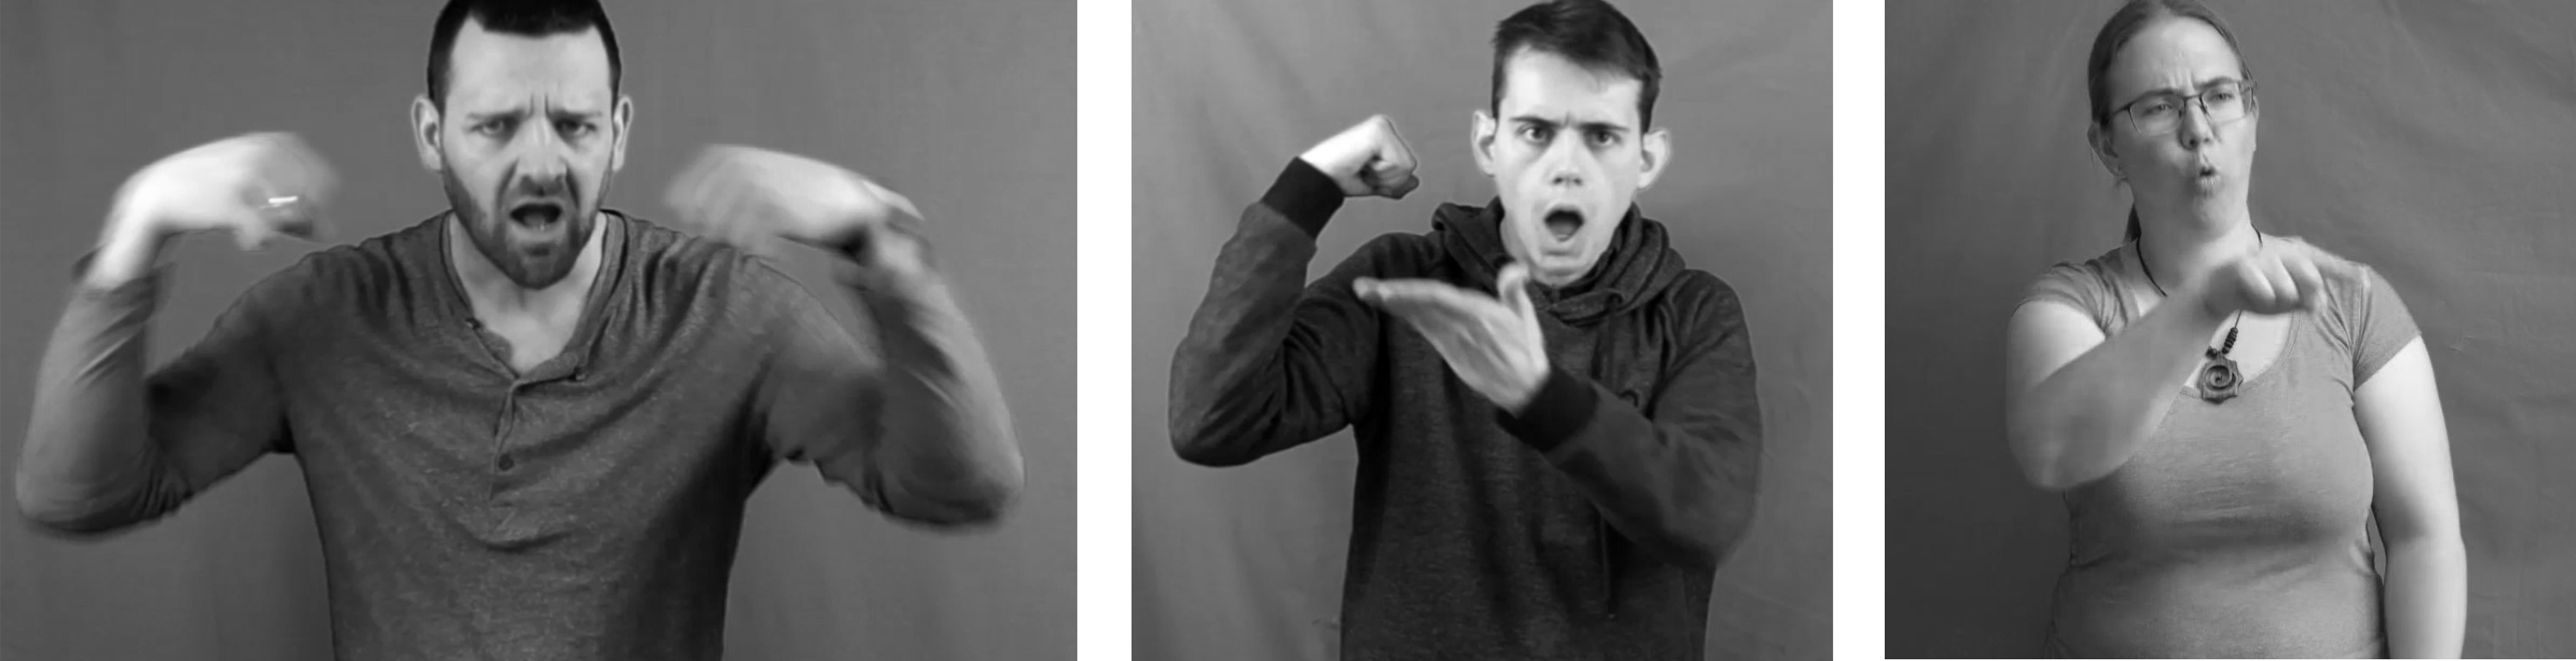
\includegraphics[width=1.0\textwidth]{imperativefacialexpressionsw.jpg}
	\caption{The non-manual markings used in imperatives.}
	\label{fig:imperativefacial}
\end{figure} 

In addition, the signs are produced faster and with more force (see also \citealt[341]{happ2014vork}). These staccato-like movements are often accompanied by rhythmically aligned head bows or head pushes (i.e., the head, often together with the upper body, is put forward and backward).\footnote{A similar observation can be made for \is{American Sign Language}American Sign Language. Although \citet{brentari2018production} mention that commands are less likely to be accompanied by head nods, their example in video number 6 clearly shows a similar head push.} To be more precise, my observation is that the bows start with the beginning of the articulation of each sign (the initial hold), arrives at its maximum at the stroke/end hold phase of the sign, and finally, in the preparation phase of the next sign, the head/body is in a reclined position again. This is illustrated in Figure \ref{fig:headmoveimp}. The Figure depicts the sentence \textsc{window always open} `Always open the window!' As can be seen, the head is reclined in the preparation phase of the sign \textsc{window} (1) and is bowed forward in the stroke/end hold phase of the sign (2 and 3). At the transition between the signs \textsc{window} and the adverb \textsc{always} (4 and 5), the head is reclined again.  At the stroke of \textsc{always} (6), the head is bowed forward again, reaching its maximum forward position at the end phase of this sign (7). The same pattern repeats on the last sign \textsc{open}. I'll take the strict alignment with each individual sign as an indication that this phenomenon is prosodic in nature (rhythmic, to be more precise). Similar to assigning word stress on each word in a spoken imperative (\textit{CLOse THE WINdow!}), the head bows seem to have an emphatic function.% As opposed to other sign languages, DGS seems to lack a manual imperative sign. 

\begin{figure}[bt]
\centering
	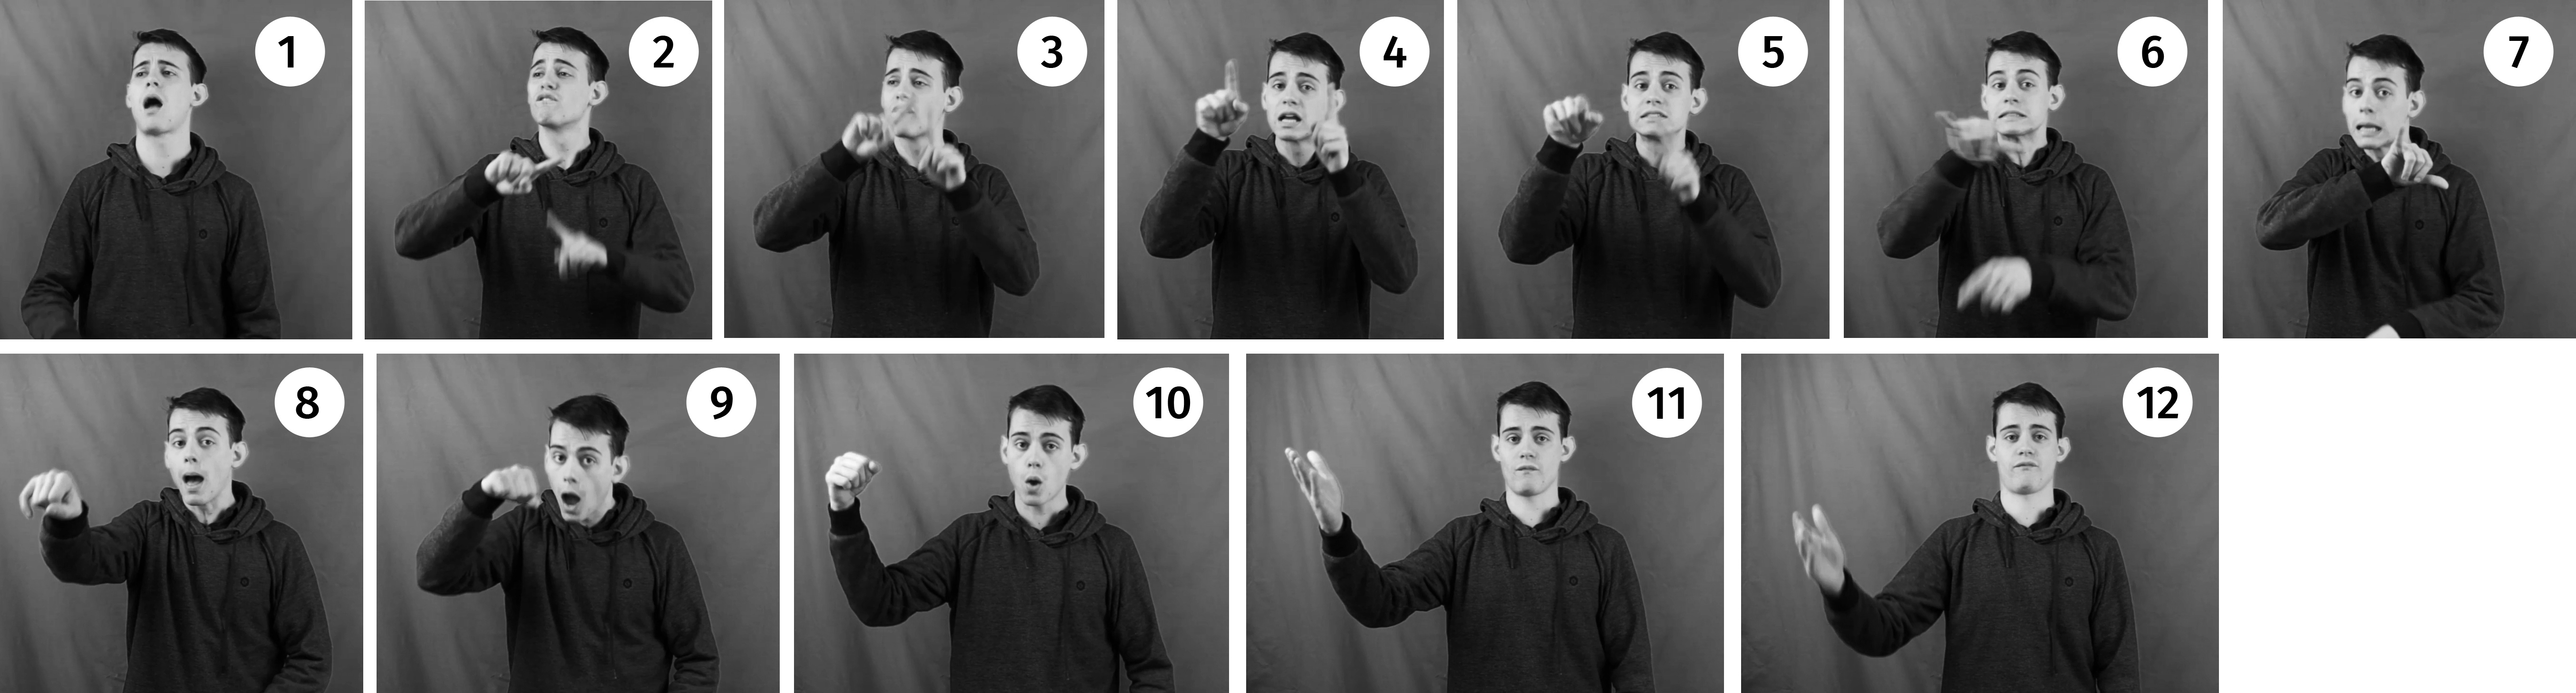
\includegraphics[width=1.0\textwidth]{imperativeheadmovementsw.jpg}
	\caption{It can often be observed that each sign receives a stress via head or body bows in imperatives.}
	\label{fig:headmoveimp}
\end{figure}

\subsubsection{An imperative sign?}
As the picture shows, sometimes a clause-final imperative sign, similar to the palm-up index sign described for \is{Italian Sign Language}Italian Sign Language in the previous section, can be observed. It remains to be investigated if it is a clear imperative marker or a gesture, but the fact that its position seems to be limited to the clause-final position -- similar to the palm-up gesture in polar interrogatives -- points in the direction of it being a sign. 

\subsubsection{Subject drop}
%Pronoun doubling and the subject position
With imperatives, the addressee of the order can be dropped, i.e., there does not have to be an overt pronoun.\footnote{But note that DGS, in general, allows subject drop.} When such a pronoun is included this is done to give the order more weight. Then, it appears in its usual subject position. Additionally, it can be doubled, just as in interrogatives\is{pronoun!doubling} 

These options are shown in (\ref{imperativedgssimple}). The first of these examples, (\ref{imperativedgssimplea}), shows a typical DGS imperative with the subject dropped. Example (\ref{imperativedgssimpleb}) illustrates that the subject can appear in an imperative. Finally, (\ref{imperativedgssimpled}) shows an instance of pronoun doubling that is, as discussed earlier, possible in polar interrogatives and imperatives in DGS.

\begin{exe}
\ex\label{imperativedgssimple}\begin{xlist} 
\ex \slg[imp]{beer drink}
%
%\ex {\hspace{10pt}imperative}   \\
%{$\overline{\textrm{\textsc{beer drink}}}$}     
\glt `Drink a beer!' \label{imperativedgssimplea}
\ex \slg[imp]{index_2 beer drink}
%
%\ex {\hspace{52pt}imperative}   \\
%{$\overline{\textrm{\textsc{index}\textsubscript{2} \textsc{beer drink}}}$}     
\glt `Drink a beer!' \label{imperativedgssimpleb}
\ex \slg[imp]{index_2 beer drink index_2}
%
%\ex {\hspace{93pt}imperative}   \\
%{$\overline{\textsc{index}\textsubscript{2} \textrm{\textsc{ beer drink} \textsc{index}\textsubscript{2}}}$}     
\glt `Drink a beer!' \label{imperativedgssimpled}
\end{xlist}
\end{exe}

\noindent In contrast to what was described for other sign languages (see the previous section), DGS does not allow proper names in imperatives. Thus, an example like the one in (\ref{ximperativesubjectslis}) is not possible.


\begin{exe}
\ex *\slg[imp]{tobias beer drink}
%\ex {\hspace{95pt}imp}   \\
%{*$\overline{\textrm{\textsc{tobias drink beer}}}$}     
\glt \textcolor{white}{*}`Tobias, drink a beer!' \label{ximperativesubjectslis}
\end{exe}

\noindent What is, in contrast, possible is to have a quantified DP in an imperative sentence (\ref{quantifieddpimp}). The position of the subject DP is, as the examples show, variable. It can either occur after a temporal adverb (that are usually found in clause-initial positions) (\ref{quantifieddpimpa}) or preceding it (\ref{quantifieddpimpb}). In the first case, the subject DP \textsc{all soldier} seems to be located in the canonical subject position. In the second case, it may be that it is located in a vocative position (and vocatives are, in general, assumed to be hosted in the highest functional structures observed so far, cf. \citealt{moro2003notes, hill2007vocatives, hill2013vocatives}). However, more research on vocatives in DGS is needed. 

\begin{exe}
\ex\label{quantifieddpimp}\begin{xlist}
\ex \slg[imp]{now all soldier hide}
%
%\ex {\hspace{110pt}imp}   \\
%{$\overline{\textrm{\textsc{now all soldier hide}}}$}     
\glt `All soldiers, hide now!' \label{quantifieddpimpa}
\ex \slg[imp]{all soldier now hide}
%
%\ex {\hspace{110pt}imp}   \\
%{$\overline{\textrm{\textsc{all soldier now hide}}}$}     
\glt `All soldiers, hide now!' \label{quantifieddpimpb}
\end{xlist}
\end{exe}

\subsubsection{The imperative verb}
\noindent Concerning the verb form, DGS behaves in an interesting way as there is no special verb form that is used in imperatives. The only difference between other sentence types might be that the verb can be produced  faster and with more force -- however, this is not only true for the verb, but for all signs in an imperative. This is probably done, for example, to give an order more stress. Verbal signs in imperatives, however, show the same agreement behavior as in other sentence types. 

Thus, verb signs used in imperatives agree at least with the object. This is illustrated on the top in Figure \ref{fig:inflectimp}. The figure shows the imperative \textit{Give him the book!} The signer's gaze is directed at the addressee when signing \textsc{book} and then follows the direction of motion of the verb sign \textsc{give} that starts in a position towards the addressee and ends at the location of the referent to whom the book should be given. Thus, the verb \textsc{give} behaves in imperatives just as in assertions. The use of \textsc{give} in an assertion is shown for the translational equivalent of the sentence \textit{Paul hopes that Otto gives him the book} below the imperative in Figure \ref{fig:inflectimp} (note that verb agreement can also be observed in what normally would be considered as infinitival complements).


\begin{figure}[bt]
\centering
	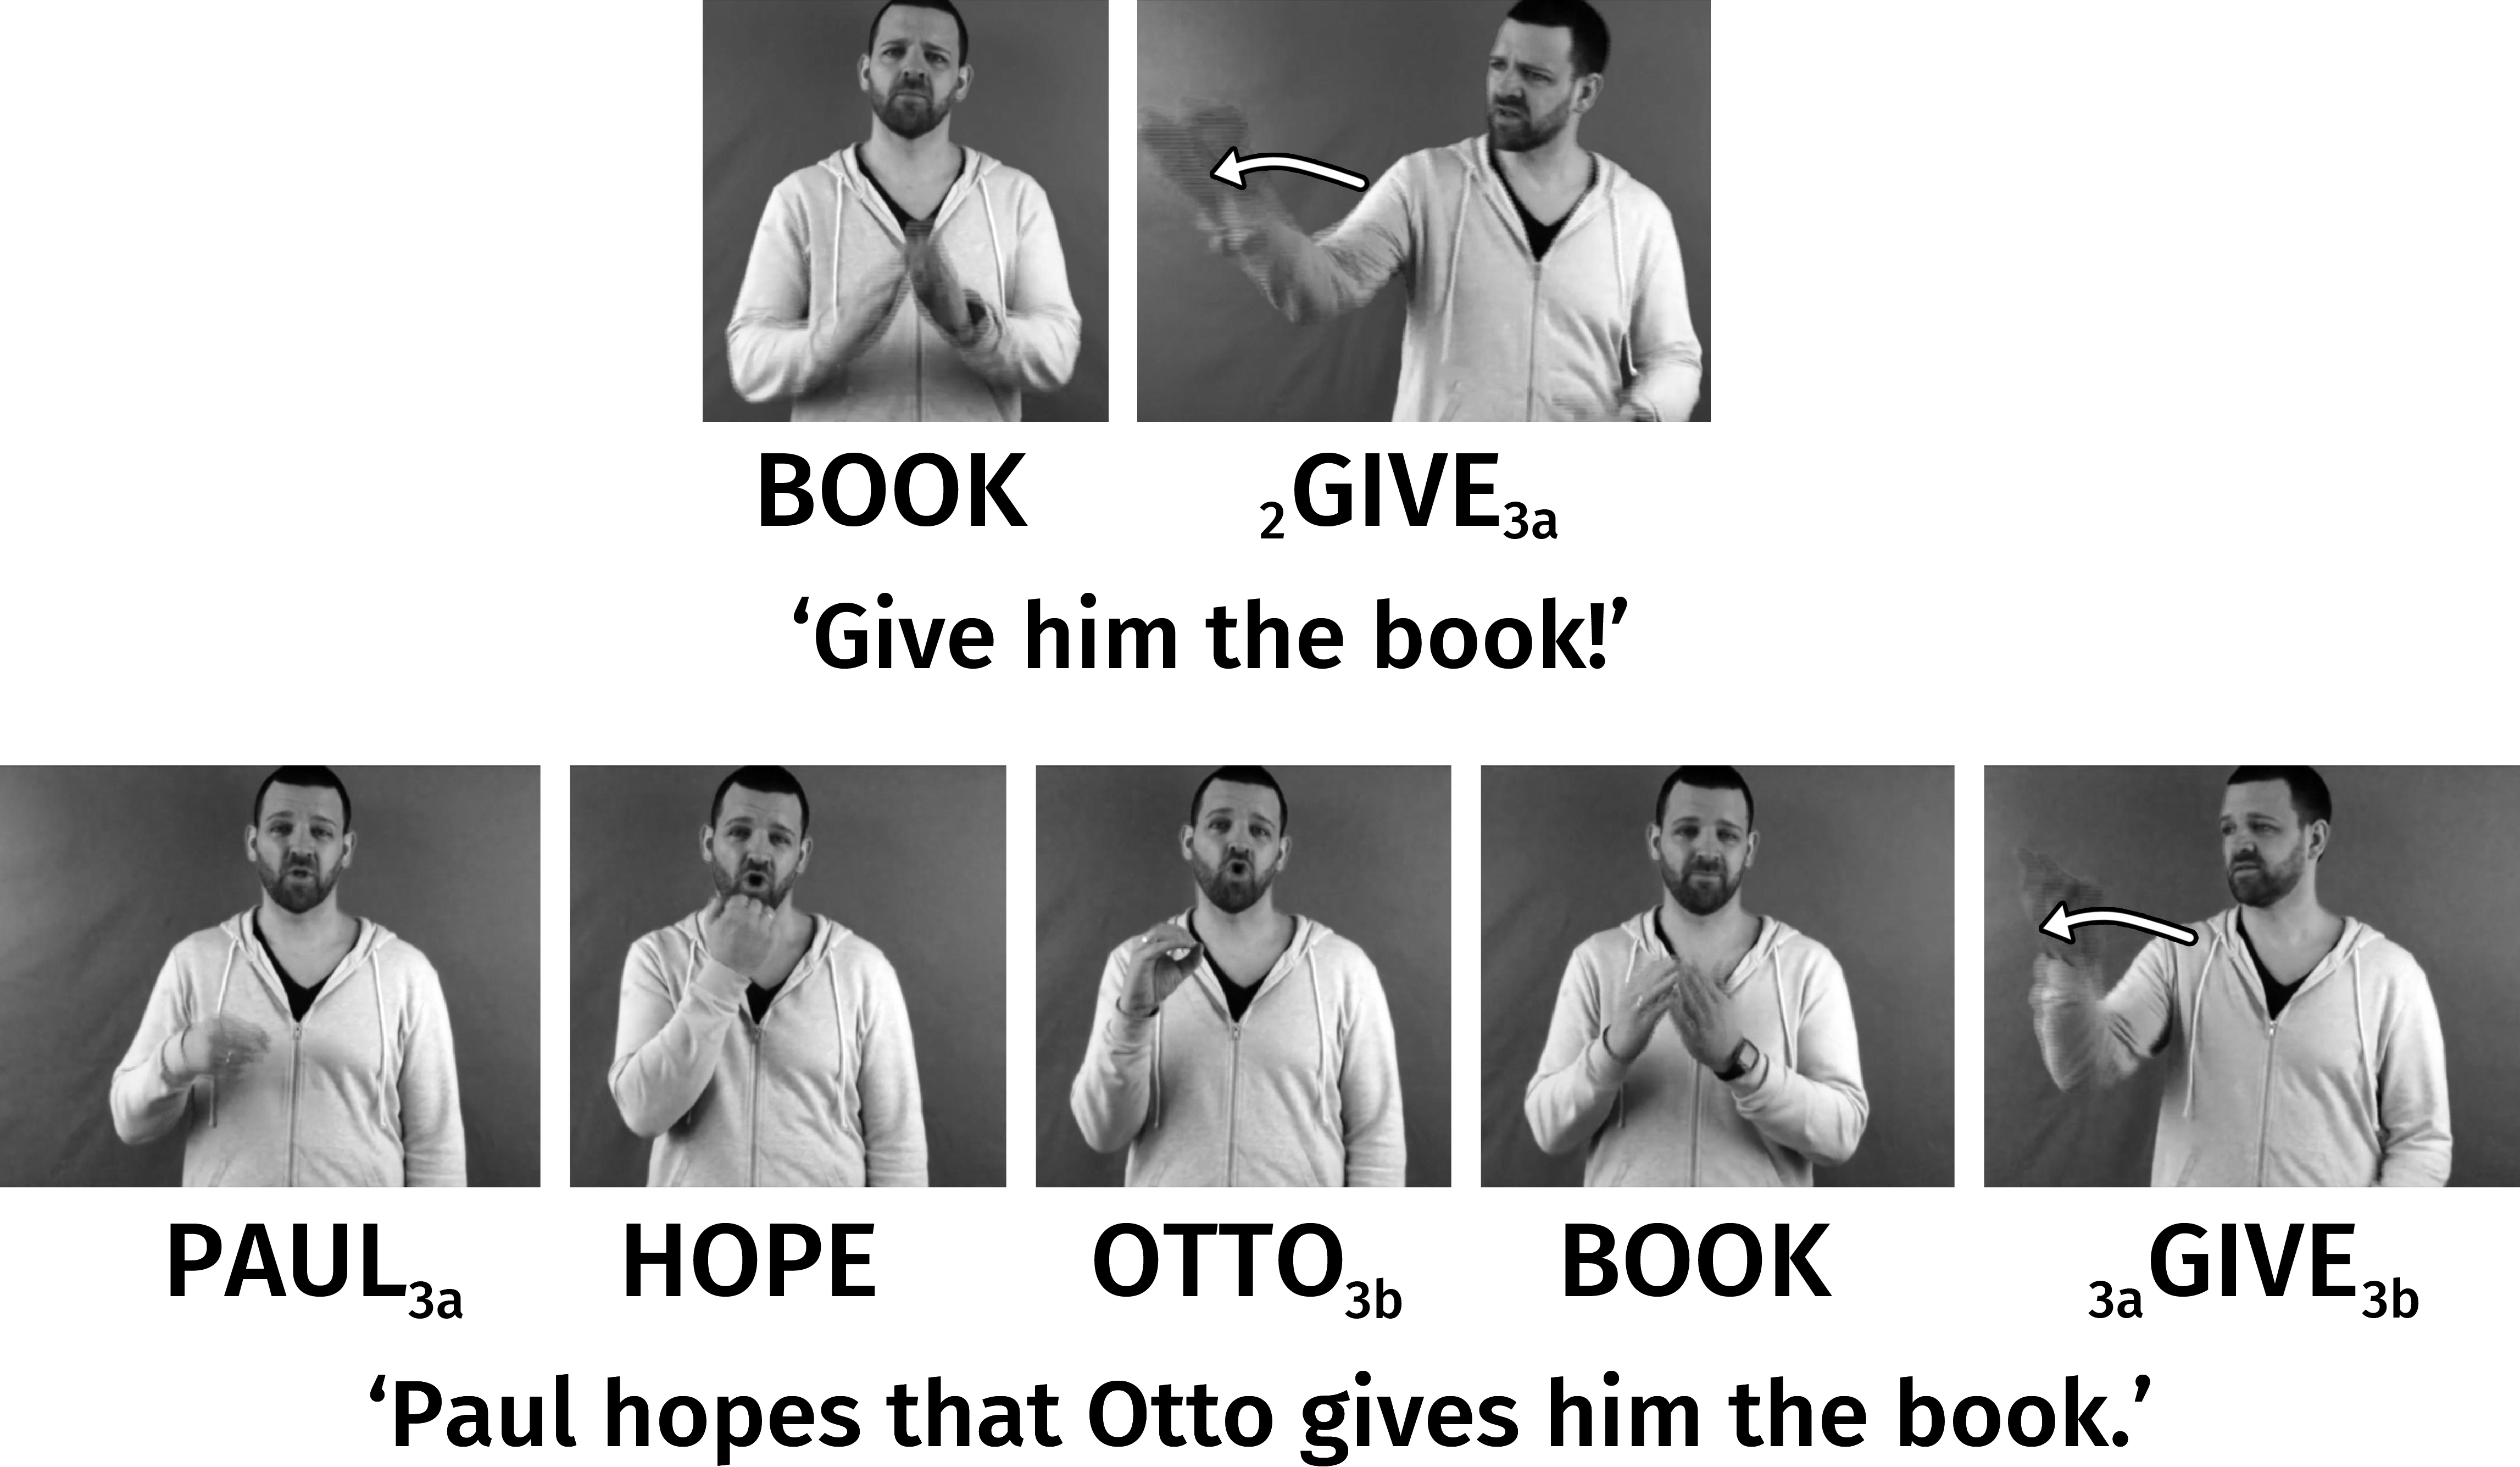
\includegraphics[width=1.0\textwidth]{inflectimpsw.jpg}
	\caption{Verbal agreement in imperatives does not differ from verbal agreement in other sentence types in DGS.}
	\label{fig:inflectimp}
\end{figure}

That verbs in imperatives show normal agreement should not be too surprising, however. Although it is usually assumed that the functional structure of imperatives is defective, several authors have found evidence that the verb in imperatives still bears its \textit{phi} features (e.g., \citealt{henry1995belfast, rupp2002syntax}). Although the imperative verb in present day English, for example, does not show any overt agreement morphology, this was different in Early Modern English as illustrated in the examples in (\ref{impearlymodernenglish}) cited by \citet[25]{rupp2002syntax}.

\begin{exe}
\ex Early Modern English \citep[25]{rupp2002syntax}\label{impearlymodernenglish}\begin{xlist} 
\ex \gll {\textit{O}} {\textit{goddesse}} {\textit{immortal}!} {Be} {\textit{helping}} {\textit{now},} {$[$\dots$]$}  \\
{O} {goddess} {immortal} {be.\textsc{2s.imp}} {helping} {now} {$[$\dots$]$} \\
\trans `O immortal goddess! You be helping now, $[$\dots$]$.' \label{ex:impearlymodernenglisha}
\ex \gll {\textit{Fy}} {\textit{on}} {\textit{yow}!} {goyth} {\textit{hence}} {\textit{Out}} {\textit{of}} {\textit{my}} {\textit{presence}}   \\
{Fie} {on} {you} {go.\textsc{2pl.imp}} {hence} {out} {of} {my} {presence} \\
\trans `Fie on you! Now (you) get out of my sight.' \label{ex:impearlymodernenglishb}
\end{xlist}
\end{exe}

\noindent Early Modern English had, as the example pair shows, a morphological contrast between singular and plural as we still see today in other languages such as German. 

\subsubsection{Negated imperatives}
%Negative imperatives
Before turning to the discussion of negated imperatives in DGS, I will make some general remarks on negation in DGS in the following side-note.\label{negationnegaation}

\is{negation|(}

\begin{digression}{Negation in DGS and the \textit{why-not} test}{}
\noindent Cross-linguistically, sign languages fall into two classes when it comes to negation, as negation can be expressed non-manually or manually. The non-manual strategy usually consists of a head-shake, the manual strategy consists of a manual negator (see \citealt{zeshan2004negation}). DGS is classified as a non-manual dominant language as a head-shake is used as the only marker to express standard negation. According to \citet[55]{pfau2016featural} there are four negation patterns in DGS that are shown in (\ref{pfauneg}). 


\begin{exe}
\ex\label{pfauneg}\begin{xlist} 
\ex \slg{poss_1 brother wine} \slg[hs]{like}
%\ex {} {\hspace{135pt}hs}  \\
%{\textsc{poss\textsubscript{1} brother wine}} {$\overline{\textrm{\textsc{like}}}$} 
\glt `My brother doesn't like wine.' \label{pfaunega}
\ex \slg{poss_1 brother} \slg[hs]{wine like}
%
%\ex {} {\hspace{134pt}hs}  \\
%{\textsc{poss\textsubscript{1} brother}} {$\overline{\textrm{\textsc{wine like}}}$} 
\glt `My brother doesn't like wine.' \label{pfaunegb}
\ex \slg{poss_1 brother wine} \slg[hs]{like neg}
%
%\ex {} {\hspace{160pt}hs}  \\
%{\textsc{poss\textsubscript{1} brother wine}} {$\overline{\textrm{\textsc{like neg}}}$} 
\glt `My brother doesn't like wine.' \label{pfaunegc}
\ex \slg{poss_1 brother} \slg[hs]{wine like neg}
%
%\ex {} {\hspace{160pt}hs}  \\
%{\textsc{poss\textsubscript{1} brother}} {$\overline{\textrm{\textsc{wine like neg}}}$} 
\glt `My brother doesn't like wine.' \label{pfaunegd}


\end{xlist}
\end{exe} 

\noindent Pfau's examples illustrate that the head shake, glossed as `hs', must at least accompany the verb (\ref{pfaunega}), but may spread over the object (\ref{pfaunegb}). For some authors, this pattern is the most neutral form of negation (e.g., \citealt{happ2014vork}). When a clause contains a head shake, the manual negator \textsc{neg} (in Pfau's transcription \textsc{not}) may optionally be used, as shown in (\ref{pfaunegc}) and (\ref{pfaunegd}). In all cases, the head shake has to be present at least over the verb (and \textsc{neg} if present).

Interestingly Southern DGS seems to behave differently from what is found in the literature. My consultants unanimously rejected examples with the head shake spreading over the object. The only option left is, thus, that the head shake accompanies the verb, as in example (\ref{pfaunega}). 

A last question concerning negation is the status of the head-shake and \textsc{neg}. Whether they are heads or phrases located in a specifier position can be tested using the \textit{why-not} test \citep{merchant2006no, zeijlstra2015morpho}. A \textit{wh}-element like \textit{why} is phrasal. Therefore it should be disallowed for a head to adjoin \textit{why} (as head-to-phrase adjunction is not possible).  A negative element that is in the specifier of NegP (i.e., an XP), in contrast, can adjoin \textit{why}:

\begin{quote}
If the sentential negative marker in a given language is phrasal (an XP, generally adverbial), it will occur in the collocation \textit{why not?}; if it is a head (an X\textdegree , generally clitic-like), it will not. \citep[20]{merchant2006no}
\end{quote}

\noindent The German negator \textit{nicht}, for example, is an XP (depending on the account either located in the specifier of NegP or a vP adjunct). As an XP it is allowed to adjoin with \textit{warum} `why' (\textit{Warum nicht?}). The negative head \textit{nein}, in contrast, cannot adjoin \textit{warum} (*\textit{Warum nein?}). Languages that use negative heads, like Italian, disallow the adjunction of a negative head particle, in Italian the particle \textit{non} to \textit{perchè} `why' (*\textit{Perchè non}). Instead, the word \textit{no} has to be used, i.e., an XP (\textit{Perchè no?}). 

Applying the \textit{why-not} test to DGS shows that a head-shake-only strategy is not allowed in the translational equivalent of \textit{why not} (\ref{whynottestdgs}). Instead, the use of the manual negator \textsc{neg} is required, as observed by \citet[56]{pfau2016featural}. These judgments were confirmed by my consultants. 

\begin{exe}
\ex\label{whynottestdgs}\begin{xlist}
\ex\label{ex:modaldoublingneg} *\slg[hs, wh]{why}
%\glll {\hspace{30pt}{}}  {\hspace{27pt}${\hspace{33pt}\underline{\textrm{\quad hn + ec}}}$} \\
%{} {\hspace{1pt}hs/wh}  \\
%{*$\overline{\textrm{\textsc{why}}}$}    
\glt \textcolor{white}{*}`Why not?'

\ex\label{ex:modaldoublingnegb} \textcolor{white}{*}\slg[hs, wh]{why neg}
%\glll {\hspace{30pt}{}}  {\hspace{27pt}${\hspace{33pt}\underline{\textrm{\quad hn + ec}}}$} \\
%{\hspace{25pt}hs/wh}  \\
%{\textcolor{white}{*}$\overline{\textrm{\textsc{why neg}}}$}    
\glt \textcolor{white}{*}`Why not?'
\end{xlist}
\end{exe}


\noindent From this we can conclude that \textsc{neg} is phrasal while the head-shake is a syntactic head (for more details see \citealt{pfau2016featural}).

 

\end{digression}
%%%%%%%%%%%%%%%%%%%%%%%%%%%%%%%%%%%%%%%%%%%%%%%%%%%%%%%%%%
%\clearpage
%%%%%%%%%%%%%%%%%%%%%%%%%%%%%%%%%%%%%%%%%%%%%%%%%%%%%%%%%%

\largerpage
\noindent Negation in negative imperatives clearly differs from negation in declaratives in DGS: while declaratives require the use of a head shake and only optionally allow for the manual negator \textsc{neg}, negative imperatives in DGS are produced via the manual negation marker \textsc{neg} only (the sign \textsc{neg} itself is obligatorily accompanied by a head shake). Negating an imperative via head shake only, in contrast, is not possible, as illustrated by the contrast in (\ref{negimpdgs}).   

\begin{exe}
\ex\label{negimpdgs}\begin{xlist} 
\ex\label{negimpdgsa} \textcolor{white}{*}\slg[imp]{window open \slg[\textup{hs}]{neg}}
\glt \textcolor{white}{*}`Don't open the window!'
\ex *\slg[imp]{window \slg[\textup{hs}]{open}}
\glt \textcolor{white}{*}`Don't open the window!'
\end{xlist}
\end{exe} 

\noindent Alternatively, another negative sign can be used to negate an imperative. This can be, for example, the sign \textsc{not-yet}. %As with \textsc{neg}, these negative signs occupy a clause-final position. 

The observation that regular negation is not allowed in DGS imperatives is in line with the idea that verb movement is blocked in languages in which negation is expressed by a head. This might be the reason why the head-shake in negative imperatives is totally absent on the verb (cf. \ref{negimpdgsa}). While DGS in this respect patterns with other languages that do not allow the regular negator in imperatives, the syntactic analysis of this phenomenon is not straightforward -- at least when it comes to standard analysis of negation in sign languages. The head-shake on the verb in non-imperative sentences was analyzed as an affix. \citet[57]{pfau2016featural}, for example, proposes the two analyses for negation in DGS shown in the trees in (\ref{ex:twoneganalysespfau}) (I slightly adapted the trees). Both model the sentence \textit{My brother doesn't like wine} from the example in (\ref{pfaunega}). The structure in (\ref{ex:twoneganalysespfaua}) allows heads and especially specifiers on both sides while the structure in (\ref{ex:twoneganalysespfaub}) is strictly antisymmetric (for the correct word order, further movement would be required in the antisymmetric structure that is not depicted).

%%%%%%%%%%%%%%%%%%%%%%%%%%%%%%%%%%%%%%%%%%%%%%%%%%%%%%%%%
%\clearpage
%%%%%%%%%%%%%%%%%%%%%%%%%%%%%%%%%%%%%%%%%%%%%%%%%%%%%%%%%

\begin{exe}
\ex\label{ex:twoneganalysespfau}
\setlength{\columnsep}{-80pt}
\begin{multicols}{2}
\begin{xlist}
\ex\label{ex:twoneganalysespfaua}
\hspace{-1.5cm}\scalebox{0.8}{
\begin{forest}
baseline=(current bounding box.north), for tree={s sep=2mm, inner sep=0, l=5mm}%s sep = Breite; l = Höhe
[{NegP} [SpecNegP [{$\left(\frac{\hfill\textrm{hs}}{\textrm{{\normalsize \textsc{neg}}}}\right)$}] ] [{ $\overline{\textrm{Neg}}$} [{ Neg\textdegree } [{ hs\textsubscript{affix}}, name=x] ] [{ vP} [{ Subject} [{ \textsc{poss}\textsubscript{1} \textsc{brother}}, roof, name=three] ] [{ VP} [{ V\textdegree } [{ \textsc{like}},name=v] ] [{ Object} [{ \textsc{wine}}, roof, name=threet]] ] ] ] ]
\draw[semithick, <-] (x.south) to [bend right=95] (v.south);
\end{forest}
}

\ex \label{ex:twoneganalysespfaub}
\scalebox{0.8}{
\begin{forest}
for tree={s sep=2mm, inner sep=0, l=5mm} %s sep = Breite; l = Höhe
[{ NegP} [{$\overline{\textrm{Neg}}$} [{ vP} [{ Subject} [{ \textsc{poss}\textsubscript{1} \textsc{brother}}, roof, name=three] ] [{ VP} [{ Object} [{ \textsc{wine}}, roof, name=threet] ] [{ V\textdegree } [{ \textsc{like}},name=v] ] ] ] [{ Neg\textdegree } [{ hs\textsubscript{affix}},name=x] ] ] [{ SpecNegP} [{ $\left(\frac{\hfill\textrm{hs}}{\textrm{{\normalsize \textsc{neg}}}}\right)$}] ] ]
\draw[semithick, <-] (x.south) to [bend right=-95] (v.south);
\end{forest}
}
\end{xlist}
\end{multicols}
\end{exe} 


%\begin{exe}
%\ex\label{ex:twoneganalysespfau}
%\begin{multicols}{2}
%\begin{xlist}
%
%\ex\label{ex:twoneganalysespfaua}
%\begin{tikzpicture}[baseline=(current bounding box.north), scale=0.4]
%\tikzset{sibling distance=0.1pt,level distance=50pt}
%\tikzset{every tree node/.style={align=left,anchor=north}}
%
%\Tree [.{\LARGE NegP} [.{\LARGE SpecNegP {$\left(\frac{\hfill\textrm{hs}}{\textrm{{\normalsize \textsc{neg}}}}\right)$}} ] [.{\LARGE $\overline{\textrm{Neg}}$} [.{\LARGE Neg\textdegree } \node(x){\LARGE hs\textsubscript{affix}}; ] [.{\LARGE vP} [.{\LARGE Subject} \edge[roof];  \node(three){\LARGE \textsc{poss}\textsubscript{1} \textsc{brother}}; ] [.{\LARGE VP} [.{\LARGE V\textdegree } \node(v){\LARGE \textsc{like}}; ] [.{\LARGE Object} \edge[roof];  \node(threet){\LARGE \textsc{wine}}; ] ] ] ] ]
%
%
%
%\draw[semithick, <-] (x.south) to [bend right=95] (v.south);
%%[.IntP [.SpecIntP ] [.{$\overline{\textrm{Int}}$} [.{Int\textdegree } ] [.FocP [.SpecFocP ] [.{$\overline{\textrm{Foc}}$} [.{Foc\textdegree } ] [.IP \edge[roof]; \node(t){\qquad\qquad}; ] ] ] ] ]
%
%\end{tikzpicture}
%
%\ex \label{ex:twoneganalysespfaub}
%
%\begin{tikzpicture}[baseline=(current bounding box.north), scale=0.4]
%\begin{scope}[xshift=-3cm]
%\tikzset{sibling distance=0.1pt,level distance=50pt}
%%\tikzset{every tree node/.style={align=left,anchor=north}}
%
%\Tree [.{\LARGE NegP} [.{\LARGE$\overline{\textrm{Neg}}$} [.{\LARGE vP} [.{\LARGE Subject} \edge[roof];  \node(three){\LARGE \textsc{poss}\textsubscript{1} \textsc{brother}}; ] [.{\LARGE VP} [.{\LARGE Object} \edge[roof];  \node(threet){\LARGE \textsc{wine}}; ] [.{\LARGE V\textdegree } \node(v){\LARGE \textsc{like}}; ] ] ] [.{\LARGE Neg\textdegree } \node(x){\LARGE hs\textsubscript{affix}}; ] ] [.{\LARGE SpecNegP} {\LARGE $\left(\frac{\hfill\textrm{hs}}{\textrm{{\normalsize \textsc{neg}}}}\right)$} ] ]
%
%\draw[semithick, <-] (x.south) to [bend right=-95] (v.south);
%%[.IntP [.SpecIntP ] [.{$\overline{\textrm{Int}}$} [.{Int\textdegree } ] [.FocP [.SpecFocP ] [.{$\overline{\textrm{Foc}}$} [.{Foc\textdegree } ] [.IP \edge[roof]; \node(t){\qquad\qquad}; ] ] ] ] ]
%\end{scope}
%\end{tikzpicture}
%
%
%
%\end{xlist}
%\end{multicols}
%\end{exe}
%

\noindent However, if we analyze the head shake as an affix, we would expect verb movement in imperatives to not be blocked. Instead, it should be possible for the affixed verb to move to the CP projection hosting the imperative feature (let's say to the head of an ImpP). Alternatively, one could propose that the verb in head-shake-only negation does not move to Neg\textdegree\ at all, but that it is activated by a covert element. The head shake then spreads over its c-command domain (that the head shake does not spread over the object in Southern DGS could be explained either by the fact that NegP is lower in the structure or that the object obligatorily moves into a higher structural position). This is in line with \citeauthor{zeijlstra2004sentential}'s (\citeyear{zeijlstra2004sentential}) proposals that languages that do not allow regular negation of imperatives are languages with a base-generated Neg\textdegree . If this is on the right track, the mechanism behind the head shake would work just as described for other cases of non-manuals previously mentioned. Concerning negated imperatives, this would mean that verb movement to Imp\textdegree\ is blocked by a covert element in Neg\textdegree . 


Taken together, I assume that with imperatives, feature checking occurs with a high CP category. This is probably done in a functional projection ImpP. As with the other sentence types, this can be modeled either by assuming a right-headed Imp\textdegree , triggering the non-manual markers or by assuming a left-branching SpecImpP to which the lexical material moves to check the features. Both accounts are in line with the fact that the palm-up index sign is found in a clause-final position. However, more research on DGS imperatives is clearly needed.

\is{negation|)}
\is{imperatives|)}


\section{Optatives}\label{opt}
\subsection{General overview}
\is{optative|(}
Optatives express wishes. They are regarded as a minor sentence type as not many languages have grammaticalized means of expressing optative mood. English often uses modal verbs (e.g., \textit{May the force be with you!}) or conditional constructions with \textit{only} (e.g., \textit{If only I had won the lottery!}). In German, optatives are often expressed using the subjunctive mood as shown in example (\ref{ex:optativegermansubjunctive}). 


\begin{exe}
\ex German \\ \gll {\textit{Hätte}} {\textit{Paul}} {\textit{doch}} {\textit{eine}} {\textit{Freundin!}}   \\
{have.\textsc{subj}} {Paul} {modal particle} {a} {girlfriend}\\
\trans `If only Paul had a girlfriend!' \label{ex:optativegermansubjunctive}
\end{exe}

\noindent While English and German use means to express optative mood that also serve different functions, there are languages that mark this category in the inflectional domain of the verb. This was, for example, the case in Ancient Greek. An example taken from \citet[216]{palmer2001mood} is given in (\ref{ex:palmer}).

\begin{exe}
\ex Greek \citep[216]{palmer2001mood} \\ \gll {\textit{ei}} {\textit{gár}} {\textit{genoíme\textlengthmark n}} {\textit{téknon,}} {\textit{antí}} {\textit{soú}} {\textit{nekrós}}          \\
{oh} {that} {become.1\textsc{sg.aor.opt}} {son} {instead.of} {you} {corpse}  \\
\trans `Oh that I might be a corpse, my child, instead of you!' \label{ex:palmer}
\end{exe}

\noindent Thus, there is cross-linguistic variation as to whether a language has grammaticalized means to express optative mood or not.

\subsection{Optatives in DGS}
The literature on optatives in DGS is extremely scarce. \citet[366]{happ2014vork} mention, without going into detail, that optative can be expressed non-manually only. Concerning my own data, signers fall into two classes. While some signers indeed allow for a non-manual-only expression of optatives, the majority of signers use a performative strategy without any non-manual markers.

%The non-manual expression of optatives used by some signers is mainly achieved with narrowed eyes.

The main non-manual marker consists of narrowing the eyes. Additionally, the head is tilted backwards. Again, the non-manuals have their intensity peak towards the end of the clause. In stark contrast to imperatives, the sign duration in optatives is slowed down.  An example of the non-manual only strategy is given in Figure \ref{optativesnonmanuals}.  

\begin{figure}[bt]
\centering
	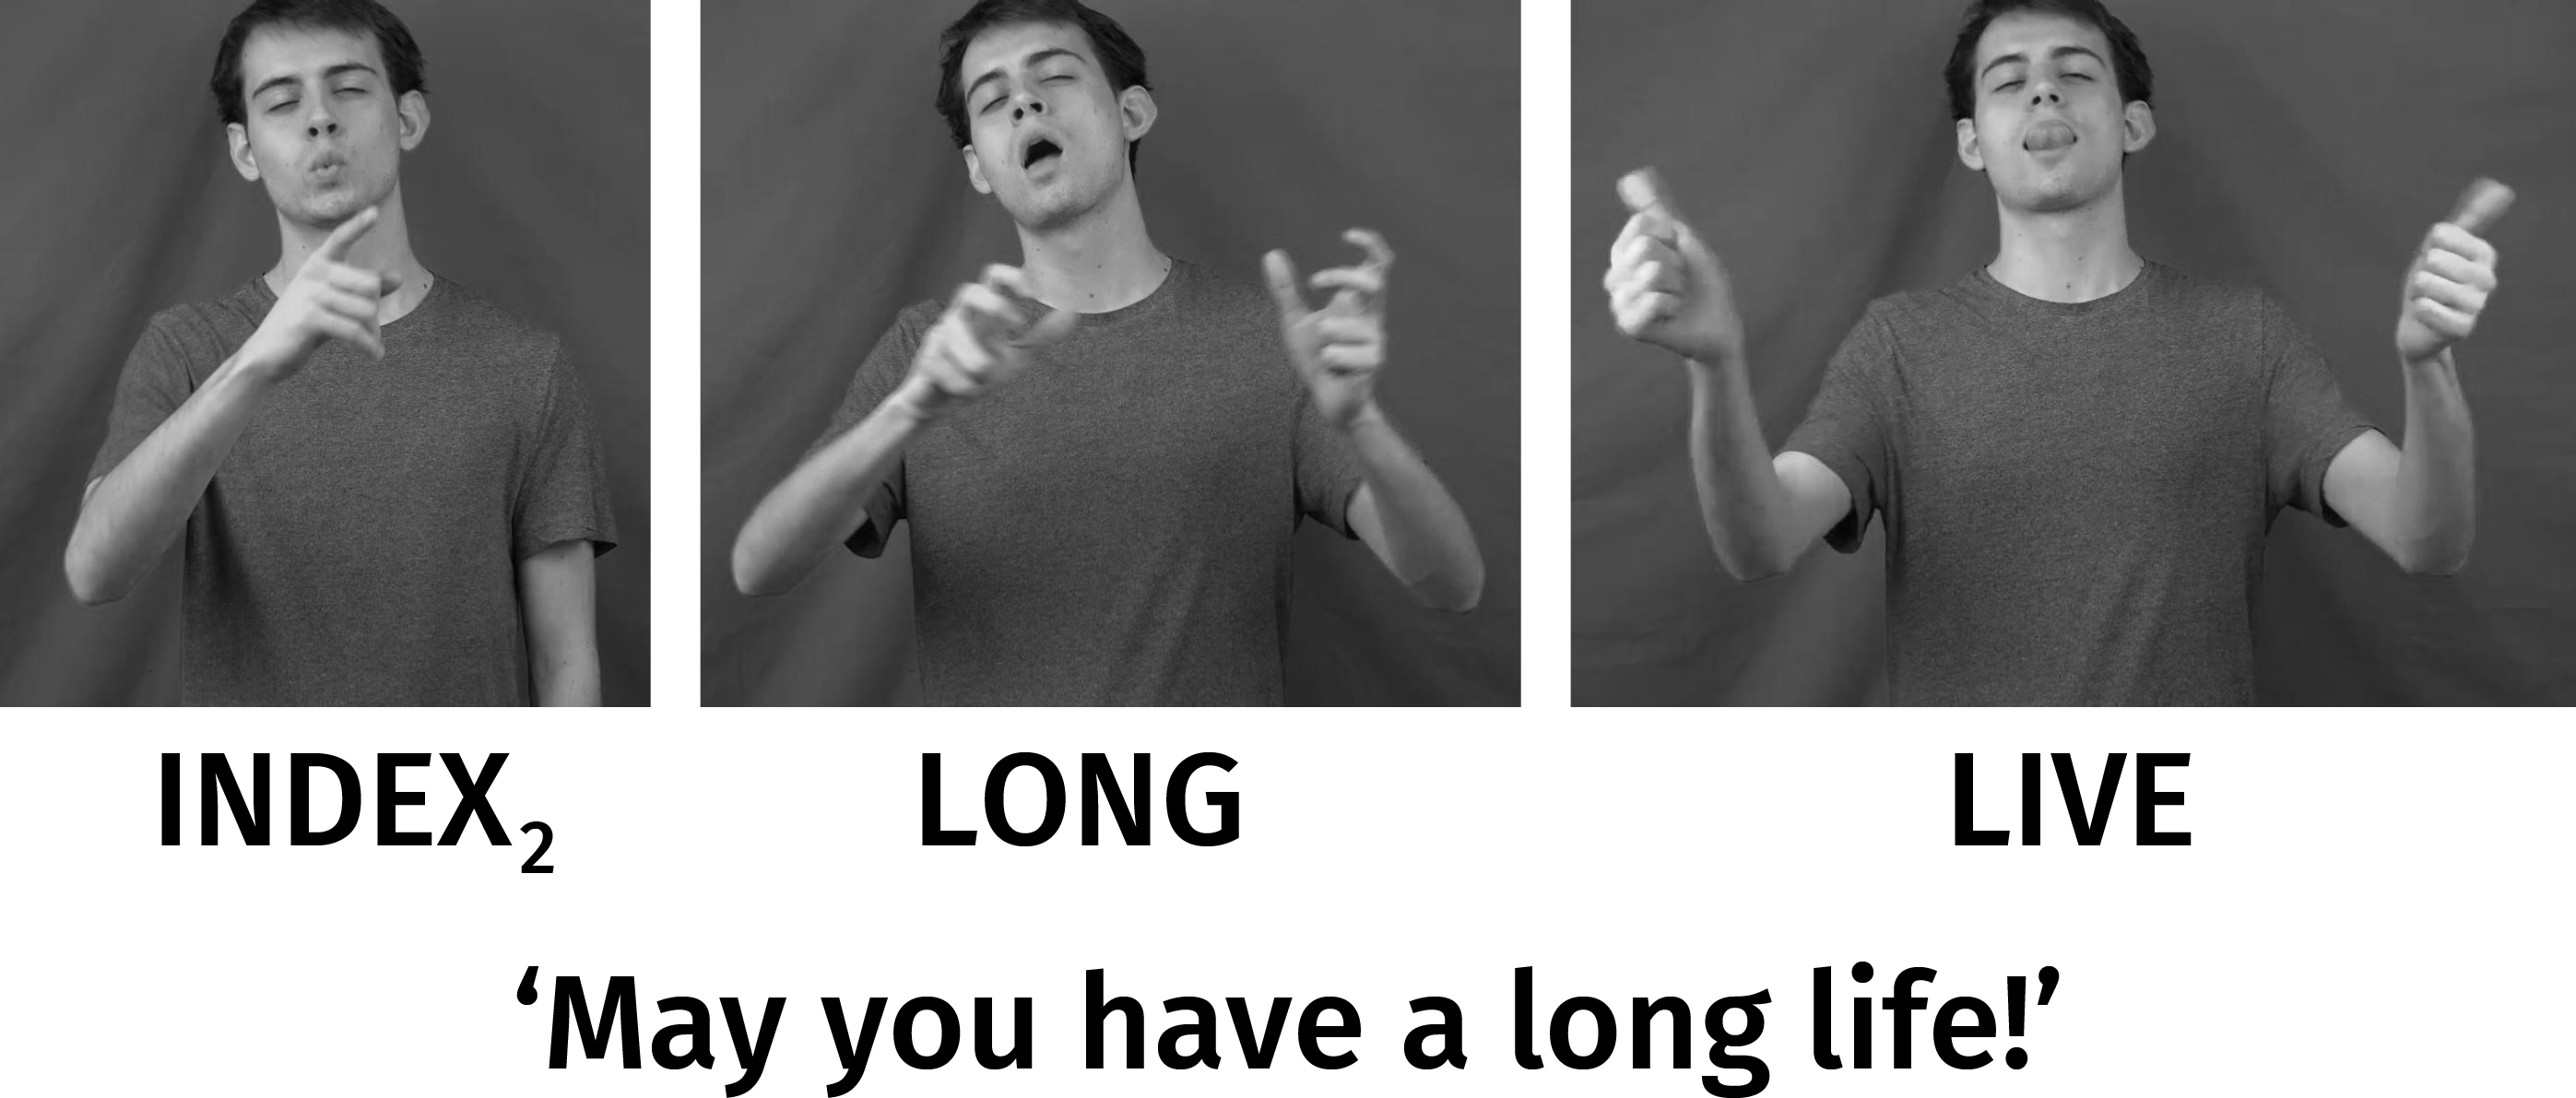
\includegraphics[width=1.0\textwidth]{optativesw.jpg}
	\caption{The main non-manual marker of optative mood consists of narrowed eyes.}
	\label{optativesnonmanuals}
\end{figure}

Most signers only allow for a strategy using performative verbs like \textsc{wish} or \textsc{like}, i.e., as there seems to be no grammaticalized way expressing them, they do not need to receive non-manual markings. This is shown in (\ref{ex:optativedgs}).

\begin{exe}

\ex{\textsc{index\textsubscript{1} wish paul there girlfriend}} 
\glt `If Paul only had a girlfriend!/I wish Paul had a girlfriend!' \label{ex:optativedgs}

\end{exe} 

\noindent It is yet unclear where this variation comes from and why some signers seem to have a grammaticalized form of an optative while others do not.

\is{optative|)}

\section{Summary and conclusion}
The goal of this chapter was to present the expression of left-peripheral categories in DGS, i.e., the higher CP domain, and to test the main hypothesis that categories with high scope are expressed using physically high articulators (see Section \ref{hypotheses} for a detailed description of the hypotheses put to test in this book). Taken together, all high CP categories find non-manual expression with the highest possible articulator, namely with the eyebrows/the eyes (or the eyebrows/eyes plus another articulator), as predicted. 

For topics, I have shown, following the literature on different kinds of topics in \is{American Sign Language}American Sign Language, that DGS exhibits at least two different types, namely those that are probably moved into left-peripheral position (i.e., integrated topics) and those that are base-generated in a slightly higher structural position (i.e., non-integrated topics). The two topic types receive different non-manual markings with the main articulators being the eyebrows in both cases. In line with previous research (e.g., \citealt{benincapol2004topic}), I have argued that non-integrated topics are structurally higher than integrated topics. The reflex of this can be seen in DGS by the fact that integrated topics have to follow non-integrated topics.

Focus in DGS is also marked non-manually. While information focus is usually not marked at all, sometimes wide-opened eyes and a short eyebrow raise can be observed, the marking of contrastive focus is subject to dialectal variation. While the signers from Baden-Württemberg tilt their heads backwards and raise their eyebrows, signers from Bavaria showed the exact opposite pattern as they put their heads and eyebrows down. Both patterns are in line with the bodily-mapping hypothesis as contrastive focus, as a structurally very high category is marked with the eyebrows. 

\largerpage
Concerning the encoding of sentence types I have shown that while declaratives are unmarked, polar interrogatives, constituent interrogatives, imperatives, as well as other, minor sentence types are marked non-manually with the eyebrows, with the non-manuals spreading over the whole clause. A general pattern that can be found in all sentence types is that the intensity peak of the non-manuals is towards the end of the clause. For polar interrogatives I have shown that their main marker is an eyebrow raise. Additionally, the head is put forward to indicate that the signer expects a response from the addressee and the head is tilted sideways. Evidence for the claim that putting the head forwards encodes the signer's expectation of a response came from the fact that it is absent in rhetorical questions. For the sideways head tilt I claimed that its function is to indicate the signer's epistemic commitment. Evidence for this claim came from the fact that the sidewards tilt is absent in inclination questions of the sort \textit{Can you pass me the salt?} in which the signer is not insecure about the proposition expressed. I will present more evidence for this claim in Section \ref{perhapsmoodirrealis} in the next chapter (see page \pageref{perhapsmoodirrealis}). Taken together, the idea is that three non-manual markers are used in polar questions to express three different functions: speech-act indication (raised eyebrows), expecting a response (head forward), and epistemic commitment (head tilt sideways). 

Following the suggestions that the palm-up gesture \textsc{p-ug} is located in the head of the InterP \citep{aboh2010sa} and that pronoun doubles are located in the head of a focus phrase \citep{de1999phrase, sandler2006sign}, I argued that a model with a right-headed InterP and a right-headed SpecFocP is more economic as it requires less movement steps to derive the fact that \textsc{p-ug} has to follow (and hence cannot precede) a focus double in polar interrogatives. However, other modeling possibilities do exist, as discussed.

\largerpage
As with polar interrogatives the non-manuals of constituent interrogatives spread over the whole clause and have their intensity peak towards the end of the clause. Instead of raising the eyebrows, the brows are lowered in this sentence type. Similar to polar interrogatives, the head is put forward to indicate that the signer is expecting a response. As was described for other sign languages, \textit{wh}-elements naturally occur in a clause-final position, although the pattern is more complex. While the unmarked position of simple \textit{wh}-phrases, like \textsc{what} or \textsc{who}, and \textit{wh}-phrases contained in a PP, like \textsc{with who}, is clause-final, complex \textit{wh}-phrases, like \textsc{which computer}, are usually found clause-initially. Another difference between simple and PP-\textit{wh}-phrases on the one hand and complex \textit{wh}-phrases on the other hand that was found was that the first two can undergo doubling, however this is not true for the latter. These differences were explained by assuming that the first two are syntactic operators while the latter are not. The distributional facts of the \textit{wh}-phrases were captured by a Split-CP model with different landing sites for different kinds of \textit{wh}-phrases. As with polar interrogatives I proposed two modeling possibilities, one allowing heads and specifiers on both sides of the tree and one antisymmetric model. Again, the non-antisymmetric model had the advantage that less movement steps are required to derive the correct surface order.

The discussion of questions was concluded by short notes on some other types of interrogatives and their encoding in DGS. I have briefly discussed alternative, degree, tag, suggestive, and rhetorical questions. While the non-manuals in alternative, degree, and tag questions are not different from polar interrogatives, a difference between information-seeking constituent questions and suggestive questions was described and it was shown that the non-manuals of rhetorical questions depend on the answer to be reconstructed. For degree questions it was shown that this question type, which often takes the form of a \textit{wh}-question in spoken languages, has its own encoding strategy in DGS which is strikingly different from \textit{wh}-questions, thus suggesting that it constitutes a type in its own right. 

Similar to the non-manuals encoding other sentence types, the non-manuals used in imperatives are furrowed brows which have their intensity peak towards the end of the clause. Similar to the palm-up gesture used in questions, a similar imperative sign that is occasionally used in a clause-final position was reported. DGS, as was shown, allows for subject drop in imperatives and proper names are generally disallowed in this sentence type. Concerning negation I have discussed that DGS follows a cross-linguistic trend in that negation in imperatives differs from negation in other sentence types. To be more precise, the manual negator \textsc{neg}, a phrasal element, has to be used in negative imperatives instead of the head-shake which has the status of a syntactic head. This observation is in line with the idea that movement of the verb to a higher CP projection hosting an imperative feature is blocked in the presence of an intervening Neg\textdegree .

The last sentence type I have briefly discussed were optatives. For this sentence type, I have shown that while most signers use performative verbs like \textsc{wish} or \textsc{like} some signers use a non-manual-only strategy. 

Taken together, the data presented in this chapter support the idea that all categories above tense find non-manual expression in DGS and are in line with the \is{bodily-mapping hypothesis}bodily-mapping hypothesis, as the highest CP functions, including topic and focus marking as well as sentence-type encoding, make use of the highest articulators available, namely the eyebrows. Note that the present chapter did not discuss the status of FinP which would be predicted to activate upper-face non-manuals. I hope that I can address the expression of FinP elements in future research. The goal of the next chapter is to shed light on the categories in the lower part of the CP and the IP-internal categories and their expression.
